% !TeX encoding = UTF-8
% !TeX program = xelatex
% !TeX spellcheck = en_US

\documentclass[degree=master]{thuthesis}
  % 学位 degree:
  %   doctor | master | bachelor | postdoc
  % 学位类型 degree-type:
  %   academic(默认)| professional
  % 语言 language
  %   chinese(默认)| english
  % 字体库 fontset
  %   windows | mac | fandol | ubuntu
  % 建议终版使用 Windows 平台的字体编译


% 论文基本配置,加载宏包等全局配置
% !TeX root = ./thuthesis-example.tex

% 论文基本信息配置

\thusetup{
  %******************************
  % 注意:
  %   1. 配置里面不要出现空行
  %   2. 不需要的配置信息可以删除
  %   3. 建议先阅读文档中所有关于选项的说明
  %******************************
  %
  % 输出格式
  %   选择打印版(print)或用于提交的电子版(electronic),前者会插入空白页以便直接双面打印
  %
  output = print,
  % 格式类型
  %   默认为论文(thesis),也可以设置为开题报告(proposal)
  % thesis-type = proposal,
  %
  % 标题
  %   可使用“\\”命令手动控制换行
  %
  title  = {固定路线中的视觉惯性定位\\方法研究},
  title* = {Research on Visual-Inertial Localization Methods for Fixed Routes},
  %
  % 学科门类
  %   1. 学术型
  %      - 中文
  %        需注明所属的学科门类,例如:
  %        哲学、经济学、法学、教育学、文学、历史学、理学、工学、农学、医学、
  %        军事学、管理学、艺术学
  %      - 英文
  %        博士:Doctor of Philosophy
  %        硕士:
  %          哲学、文学、历史学、法学、教育学、艺术学门类,公共管理学科
  %          填写“Master of Arts“,其它填写“Master of Science”
  %   2. 专业型
  %      直接填写专业学位的名称,例如:
  %      教育博士、工程硕士等
  %      Doctor of Education, Master of Engineering
  %   3. 本科生不需要填写
  %
  degree-category  = {工学硕士},
  degree-category* = {Master of Science},
  %
  % 培养单位
  %   填写所属院系的全名
  %
  department = {深圳国际研究生院},
  %
  % 学科
  %   1. 研究生学术型学位,获得一级学科授权的学科填写一级学科名称,其他填写二级学科名称
  %   2. 本科生填写专业名称,第二学位论文需标注“(第二学位)”
  %
  discipline  = {大数据技术与工程},
  discipline* = {Big Data Technology and Engineering},
  %
  % 专业领域
  %   1. 设置专业领域的专业学位类别,填写相应专业领域名称
  %   2. 2019 级及之前工程硕士学位论文,在 `engineering-field` 填写相应工程领域名称
  %   3. 其他专业学位类别的学位论文无需此信息
  %
  % professional-field  = {计算机技术},
  % professional-field* = {Computer Technology},
  %
  % 姓名
  %
  author  = {薛林松},
  author* = {Xue Linsong},
  %
  % 学号
  % 仅当书写开题报告时需要(同时设置 `thesis-type = proposal')
  %
  % student-id = {2000310000},
  %
  % 指导教师
  %   中文姓名和职称之间以英文逗号“,”分开,下同
  %
  supervisor  = {张凯, 副教授},
  supervisor* = {Associate Professor Zhang Kai},
  %
  % 副指导教师
  %
  % associate-supervisor  = {陈文光, 教授},
  % associate-supervisor* = {Professor Chen Wenguang},
  %
  % 联合指导教师
  %
  % co-supervisor  = {某某某, 教授},
  % co-supervisor* = {Professor Mou Moumou},
  %
  % 日期
  %   使用 ISO 格式;默认为当前时间
  %
  % date = {2019-07-07},
  %
  % 是否在中文封面后的空白页生成书脊(默认 false)
  %
  include-spine = false,
  %
  % 密级和年限
  %   秘密, 机密, 绝密
  %
  % secret-level = {秘密},
  % secret-year  = {10},
  %
  % 博士后专有部分
  %
  % clc                = {分类号},
  % udc                = {UDC},
  % id                 = {编号},
  % discipline-level-1 = {计算机科学与技术},  % 流动站(一级学科)名称
  % discipline-level-2 = {系统结构},          % 专业(二级学科)名称
  % start-date         = {2011-07-01},        % 研究工作起始时间
}

% 载入所需的宏包

% 定理类环境宏包
\usepackage{amsthm}
% 也可以使用 ntheorem
% \usepackage[amsmath,thmmarks,hyperref]{ntheorem}

\thusetup{
  %
  % 数学字体
  % math-style = GB,  % GB | ISO | TeX
  math-font  = xits,  % stix | xits | libertinus
}

% 可以使用 nomencl 生成符号和缩略语说明
% \usepackage{nomencl}
% \makenomenclature

% 表格加脚注
\usepackage{threeparttable}

% 表格中支持跨行
\usepackage{multirow}

% 固定宽度的表格。
% \usepackage{tabularx}

% 跨页表格
\usepackage{longtable}

% 算法
\usepackage{algorithm}
\usepackage{algorithmic}

% 量和单位
\usepackage{siunitx}

% 参考文献使用 BibTeX + natbib 宏包
% 顺序编码制
\usepackage[sort]{natbib}
\bibliographystyle{thuthesis-numeric}

% 著者-出版年制
% \usepackage{natbib}
% \bibliographystyle{thuthesis-author-year}

% 生命科学学院要求使用 Cell 参考文献格式(2023 年以前使用 author-date 格式)
% \usepackage{natbib}
% \bibliographystyle{cell}

% 本科生参考文献的著录格式
% \usepackage[sort]{natbib}
% \bibliographystyle{thuthesis-bachelor}

% 参考文献使用 BibLaTeX 宏包
% \usepackage[style=thuthesis-numeric]{biblatex}
% \usepackage[style=thuthesis-author-year]{biblatex}
% \usepackage[style=gb7714-2015]{biblatex}
% \usepackage[style=apa]{biblatex}
% \usepackage[style=mla-new]{biblatex}
% 声明 BibLaTeX 的数据库
% \addbibresource{ref/refs.bib}

% 定义所有的图片文件在 figures 子目录下
\graphicspath{{figures/}}

% 数学命令
\makeatletter
\newcommand\dif{%  % 微分符号
  \mathop{}\!%
  \ifthu@math@style@TeX
    d%
  \else
    \mathrm{d}%
  \fi
}
\makeatother

% hyperref 宏包在最后调用
\usepackage{hyperref}

\usepackage{graphicx}
\usepackage{subcaption}
\usepackage{tikz}
\usepackage{gensymb}
\usepackage{colortbl}
\usepackage{xr}

\allowdisplaybreaks


\begin{document}

% 封面
\maketitle

% 学位论文指导小组、公开评阅人和答辩委员会名单
% 本科生不需要
% !TeX root = ../thuthesis-example.tex

\begin{committee}[name={学位论文公开评阅人和答辩委员会名单}]

  \newcolumntype{C}[1]{@{}>{\centering\arraybackslash}p{#1}}

  % \section*{指导小组名单}

  % \begin{center}
  %   \begin{tabular}{C{3cm}C{3cm}C{9cm}@{}}
  %     李XX & 教授     & 清华大学 \\
  %     王XX & 副教授   & 清华大学 \\
  %     张XX & 助理教授 & 清华大学 \\
  %   \end{tabular}
  % \end{center}


  \section*{公开评阅人名单}

  \begin{center}
    \begin{tabular}{C{3cm}C{3cm}C{9cm}@{}}
      董宇涵 & 副教授   & 清华大学深圳国际研究生院                    \\
      何南鹰 & 高级工程师 & 上海轮上科技有限公司                    \\
    \end{tabular}
  \end{center}


  \section*{答辩委员会名单}

  \begin{center}
    \begin{tabular}{C{2.75cm}C{2.98cm}C{3.63cm}C{5.63cm}@{}}
      主席 & 金欣                  & 教授                    & 清华大学深圳国际研究生院       \\
      委员 & 董宇涵                  & 副教授                    & 清华大学深圳国际研究生院       \\
          % & \multirow{2}{*}{杨XX} & \multirow{2}{*}{研究员} & 中国XXXX科学院 \\
          % &                       &                         & XXXXXXX研究所  \\
          & 王智                  & 副教授                    & 清华大学深圳国际研究生院       \\
          & 李轶                  & 副教授                  & 清华大学深圳国际研究生院       \\
          & 冯文森                &  主任工程师              & 华为技术有限公司 \\
      秘书 &   李亚南                &   助理研究员            & 清华大学深圳国际研究生院       \\
    \end{tabular}
  \end{center}

\end{committee}



% 也可以导入 Word 版转的 PDF 文件
% \begin{committee}[file=figures/committee.pdf]
% \end{committee}


% 使用授权的说明
% 本科生开题报告不需要
\copyrightpage
% 将签字扫描后授权文件 scan-copyright.pdf 替换原始页面
% \copyrightpage[file=scan-copyright.pdf]

\frontmatter
% !TeX root = ../thuthesis-example.tex

% 中英文摘要和关键字

\begin{abstract}
  近年来,固定路线中运行的车辆、机器人等智能体越来越受到研究者关注,而定位是这类智能体的基础性功能之一,因此固定路线中的定位有着重要的研究意义和应用价值。以往的定位方法一般需要使用高精度的卫星信号或高成本的传感器来实现精确的定位功能,这些昂贵且需要精心维护的设备限制了低成本固定路线智能体的应用。
  
  为了使用低成本传感器完成较高精度的定位任务,本文提出了一种使用视觉惯性信息的固定路线定位系统,该系统涵盖了从建图到定位的完整流程,并分别从离线建图、里程计、地图定位三个方面针对现有方法中的设计问题进行改进:

  (1) 现有的建图方法中存在着精度与成本的矛盾,低成本的建图方法,例如同步定位与建图,往往因为在线建图的局部优化限制而存在精度劣势。针对这一问题本文设计了一种以运动结构恢复(Structure from Motion, SfM)为基础并融合了高精度全局信息的离线建图模块。这一模块结合了SfM的全局优化精度优势和全局信息所提供的尺度信息,能够恢复出高精度且具有真实尺度的视觉点云地图。

  (2) 现有的基于通用场景设计的视觉惯性里程计(Visual-Inertial Odometry, VIO),忽略了车辆和轮式机器人运动模式中的先验知识。针对这一问题本文设计了一种基于车身运动模式感知的伪观测视觉惯性里程计(Pseudo Obsevation Visual-Inertial Odometry, PO-VIO)模块。这一模块根据车身运动模式来构建合理的伪观测约束,基于伪观测约束来估计车身与惯性传感器的标定参数,联合优化标定参数与车身状态量,能够估计出更为合理且更高精度的车身状态。

  (3) 现有的地图定位方法普遍将定位问题看作是基于地图观测的最大似然估计问题,这一做法忽略了地图本身存在的误差。针对这一问题本文设计了一种基于最大后验概率估计的地图定位模块。这一模块将地图点的误差建模为以其空间坐标为中心的三维高斯分布,并基于这一先验概率分布进行位置和姿态的最大后验概率估计,有效减小了建图误差带来的定位误差。

  本文所提出的系统在3个公开数据集上进行了测试,论证了本文所提出系统的有效性,并通过消融实验分析了各种设计的效果。实验表明,本文所提出的固定路线中的视觉惯性定位系统有着较高的定位精度,在理想场景下可以达到厘米级的定位精度,并且可以适应天气、光照变化等环境因素改变的场景。

  % 关键词用“英文逗号”分隔,输出时会自动处理为正确的分隔符
  \thusetup{
    keywords = {固定路线, 状态估计, 同步定位与建图, 视觉惯性里程计},
  }
\end{abstract}

\begin{abstract*}
  In recent years, intelligent agents operating on fixed routes—such as vehicles and robots—have attracted increasing attention due to the fundamental role of localization in their operation. However, conventional localization methods typically rely on high-precision satellite signals or expensive sensors, limiting the application of low-cost fixed-route systems.

  To achieve high-accuracy localization with low-cost sensors, this paper presents a visual–inertial localization system tailored for fixed-route applications. The system encompasses a complete pipeline from mapping to localization and introduces targeted improvements in three key areas:

  (1) Existing mapping methods face a trade-off between accuracy and cost. Low-cost mapping approaches, such as simultaneous localization and mapping (SLAM), often suffer from accuracy limitations due to the inherent local optimization in online mapping. To overcome this issue, we design an offline mapping module based on Structure from Motion (SfM) that integrates high-precision global information. This module leverages the global optimization benefits of SfM and the scale information provided by global data to reconstruct high-accuracy visual point cloud maps with real-world scale.

  (2) Conventional VIO systems designed for general scenarios typically overlook the prior knowledge inherent in the motion patterns of vehicles and wheeled robots. To address this limitation, we propose a pseudo-observation visual–inertial odometry (PO-VIO) module based on vehicle motion pattern perception. This module constructs appropriate pseudo-observation constraints derived from vehicle dynamics to estimate the calibration parameters between the vehicle body and the inertial sensor. By jointly optimizing these calibration parameters and the vehicle state, the system achieves more accurate and reliable vehicle motion estimates.

  (3) Most existing map-based localization methods treat the problem as one of maximum likelihood estimation based solely on map observations, thereby neglecting inherent map errors. To mitigate this, we design a map-based localization module based on maximum a posteriori (MAP) estimation. In this approach, the error associated with each map point is modeled as a three-dimensional Gaussian distribution centered on its spatial coordinates. This probabilistic modeling is then employed to perform MAP estimation of both position and orientation, effectively reducing localization errors caused by mapping inaccuracies.

  The proposed system is evaluated on three publicly available datasets, and ablation studies are conducted to assess the contributions of the individual components. Experimental results demonstrate that the visual–inertial localization system achieves high localization accuracy—reaching centimeter-level precision under ideal conditions—and robustly adapts to environmental variations such as changes in weather and lighting.

  % Use comma as separator when inputting
  \thusetup{
    keywords* = {fixed route, state estimation, SLAM, VIO},
  }
\end{abstract*}


% 目录
\tableofcontents

% 插图和附表清单
% 本科生的插图索引和表格索引需要移至正文之后、参考文献前
% \listoffiguresandtables  % 插图和附表清单(仅限研究生)
\listoffigures           % 插图清单
\listoftables            % 附表清单

% 符号对照表
% !TeX root = ../thuthesis-example.tex

\begin{denotation}[3cm]
  \item[GNSS] 卫星导航系统(Global Navigation Satellite System)
  \item[PPP] 精密单点定位(Precise Point Positioning)
  \item[RTK] 实时动态定位(Real-Time Kinematic)
  \item[SLAM] 同步定位与地图创建(Simultaneous Localization And Mapping)
  \item[EKF] 扩展卡尔曼滤波器(Extended Kalman Filter)
  \item[BA] 光束法平差(Bundle Adjustment) 
  \item[IMU] 惯性测量单元(Inertial Measurement Unit)
  \item[VO] 视觉里程计(Visual Odometry)
  \item[VIO] 视觉惯性里程计(Visual-Inertial Odometry)   
  \item[SfM] 运动恢复结构(Structure from Motion) 
  \item[Sim3] 三维相似变换(Similarity Transformation in 3D) 
  \item[SO(3)] 三维旋转群(Special Orthogonal Group)
  \item[SE(3)] 三维特殊欧氏群(Special Euclidean Group)
  \item[CNN] 卷积神经网络(Convolutional Neural Network)
  \item[TCN] 时间卷积神经网络(Temporal Convolutional Neural Network) 
  \item[MAP] 最大后验概率(Maximum A Posteriori)
  \item[ML] 最大似然(Maximum Likelihood) 
\end{denotation}



% 也可以使用 nomencl 宏包,需要在导言区
% \usepackage{nomencl}
% \makenomenclature

% 在这里输出符号说明
% \printnomenclature[3cm]

% 在正文中的任意为都可以标题
% \nomenclature{PI}{聚酰亚胺}
% \nomenclature{MPI}{聚酰亚胺模型化合物,N-苯基邻苯酰亚胺}
% \nomenclature{PBI}{聚苯并咪唑}
% \nomenclature{MPBI}{聚苯并咪唑模型化合物,N-苯基苯并咪唑}
% \nomenclature{PY}{聚吡咙}
% \nomenclature{PMDA-BDA}{均苯四酸二酐与联苯四胺合成的聚吡咙薄膜}
% \nomenclature{MPY}{聚吡咙模型化合物}
% \nomenclature{As-PPT}{聚苯基不对称三嗪}
% \nomenclature{MAsPPT}{聚苯基不对称三嗪单模型化合物,3,5,6-三苯基-1,2,4-三嗪}
% \nomenclature{DMAsPPT}{聚苯基不对称三嗪双模型化合物(水解实验模型化合物)}
% \nomenclature{S-PPT}{聚苯基对称三嗪}
% \nomenclature{MSPPT}{聚苯基对称三嗪模型化合物,2,4,6-三苯基-1,3,5-三嗪}
% \nomenclature{PPQ}{聚苯基喹噁啉}
% \nomenclature{MPPQ}{聚苯基喹噁啉模型化合物,3,4-二苯基苯并二嗪}
% \nomenclature{HMPI}{聚酰亚胺模型化合物的质子化产物}
% \nomenclature{HMPY}{聚吡咙模型化合物的质子化产物}
% \nomenclature{HMPBI}{聚苯并咪唑模型化合物的质子化产物}
% \nomenclature{HMAsPPT}{聚苯基不对称三嗪模型化合物的质子化产物}
% \nomenclature{HMSPPT}{聚苯基对称三嗪模型化合物的质子化产物}
% \nomenclature{HMPPQ}{聚苯基喹噁啉模型化合物的质子化产物}
% \nomenclature{PDT}{热分解温度}
% \nomenclature{HPLC}{高效液相色谱(High Performance Liquid Chromatography)}
% \nomenclature{HPCE}{高效毛细管电泳色谱(High Performance Capillary lectrophoresis)}
% \nomenclature{LC-MS}{液相色谱-质谱联用(Liquid chromatography-Mass Spectrum)}
% \nomenclature{TIC}{总离子浓度(Total Ion Content)}
% \nomenclature{\textit{ab initio}}{基于第一原理的量子化学计算方法,常称从头算法}
% \nomenclature{DFT}{密度泛函理论(Density Functional Theory)}
% \nomenclature{$E_a$}{化学反应的活化能(Activation Energy)}
% \nomenclature{ZPE}{零点振动能(Zero Vibration Energy)}
% \nomenclature{PES}{势能面(Potential Energy Surface)}
% \nomenclature{TS}{过渡态(Transition State)}
% \nomenclature{TST}{过渡态理论(Transition State Theory)}
% \nomenclature{$\increment G^\neq$}{活化自由能(Activation Free Energy)}
% \nomenclature{$\kappa$}{传输系数(Transmission Coefficient)}
% \nomenclature{IRC}{内禀反应坐标(Intrinsic Reaction Coordinates)}
% \nomenclature{$\nu_i$}{虚频(Imaginary Frequency)}
% \nomenclature{ONIOM}{分层算法(Our own N-layered Integrated molecular Orbital and molecular Mechanics)}
% \nomenclature{SCF}{自洽场(Self-Consistent Field)}
% \nomenclature{SCRF}{自洽反应场(Self-Consistent Reaction Field)}



% 正文部分
\mainmatter
% !TeX root = ../thuthesis-example.tex

\chapter{绪论}

本章节分析了现有的固定路线定位技术的研究背景和研究意义,介绍了国内外关于视觉惯性定位和地图辅助定位的研究现状,并指出了现有研究的不足之处。本章通过论述核心研究内容,提炼出了文章的创新之处。


\section{课题背景}
近年来,汽车和机器人的智能化是炙手可热的研究和应用方向,而固定路线下运行的智能汽车和机器人是其中的一个重要研究方向。相较于通用智能,在固定路线下应用的智能化技术更容易实现,因此也涌现了一批类似于无人驾驶公交车\cite{stephen2023driverless}、智驾汽车通勤模式\cite{xin2023xinchuxing}、变电站巡检车\cite{song2020xinhuawang}、矿山无人运输机器人\cite{li2023keji}等应用场景,如图\ref{fig:apply}。在这些应用中,汽车和机器人运行在提前设置好的固定路线上,通过自身所具备感知能力对环境做出反馈,完成规划、导航等更复杂的任务。而在感知能力中,定位是最基础但是却最关键的感知能力之一,定位系统是智能汽车和机器人运行的最基础系统之一。因此,固定路线中的精确定位是一项具有较高实用价值的基础性研究,只有实现了高精度的定位,才能确保复杂任务的可靠实施,才能保证整个智能体的安全。
\begin{figure}[htbp]
  \centering
  \begin{subfigure}[b]{0.45\textwidth}
      \centering
      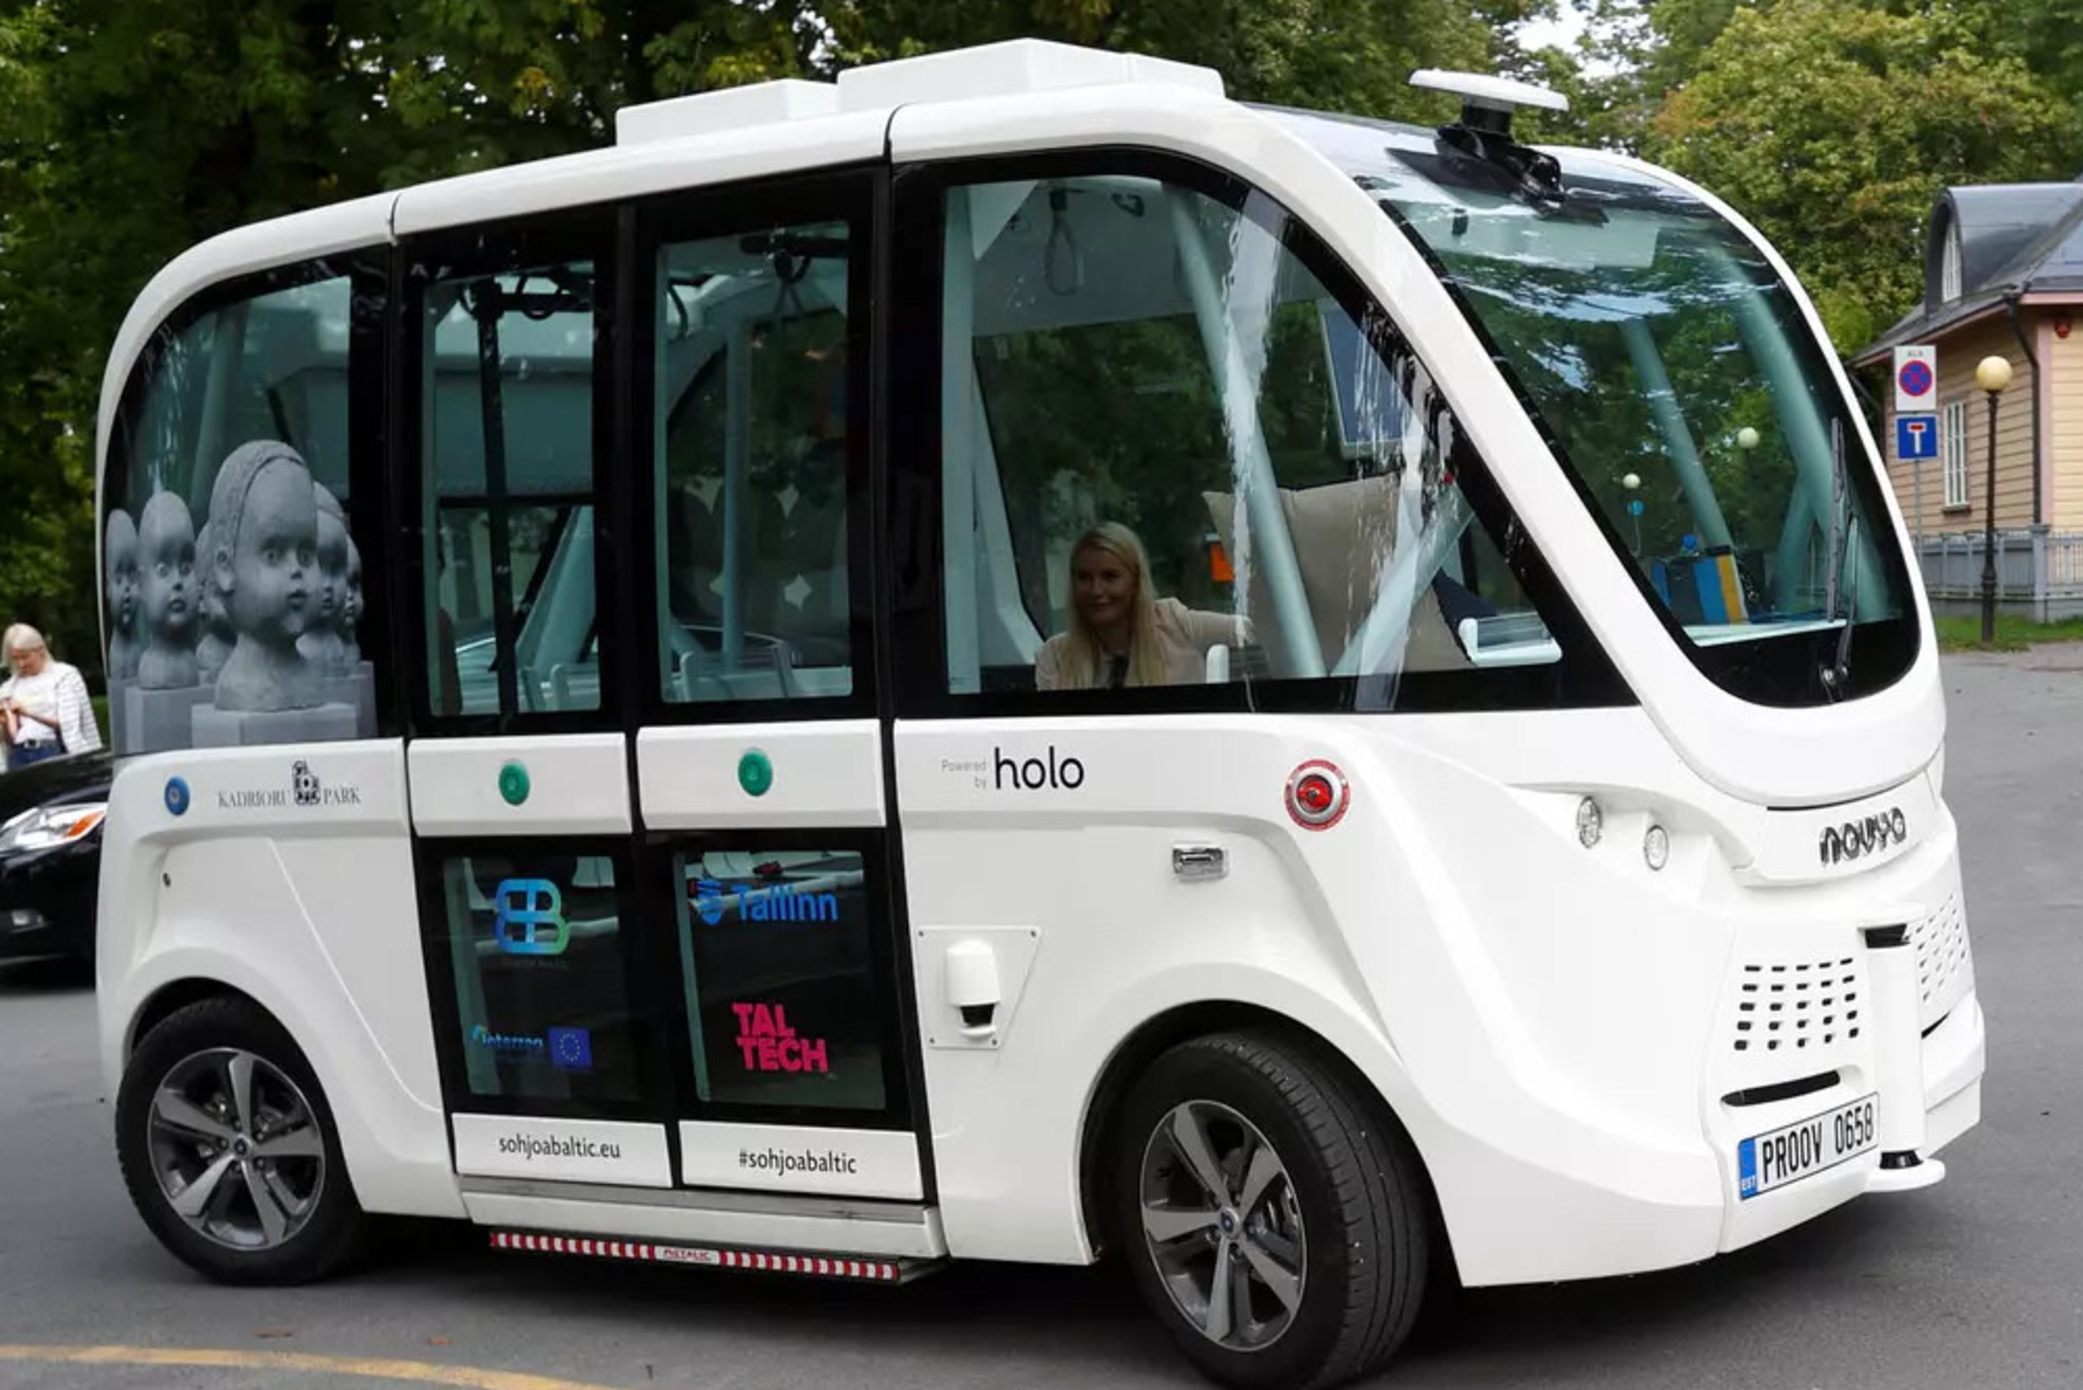
\includegraphics[width=\textwidth]{Apply1.pdf}
      \caption{无人驾驶公交车\cite{stephen2023driverless}}
      \label{fig:apply_sub1}
  \end{subfigure}
  \begin{subfigure}[b]{0.45\textwidth}
      \centering
      
\includegraphics[width=\textwidth]{Apply2.pdf}
      \caption{智驾汽车通勤模式\cite{xin2023xinchuxing}}
      \label{fig:apply_sub2}
  \end{subfigure}
  \begin{subfigure}[b]{0.45\textwidth}
      \centering
      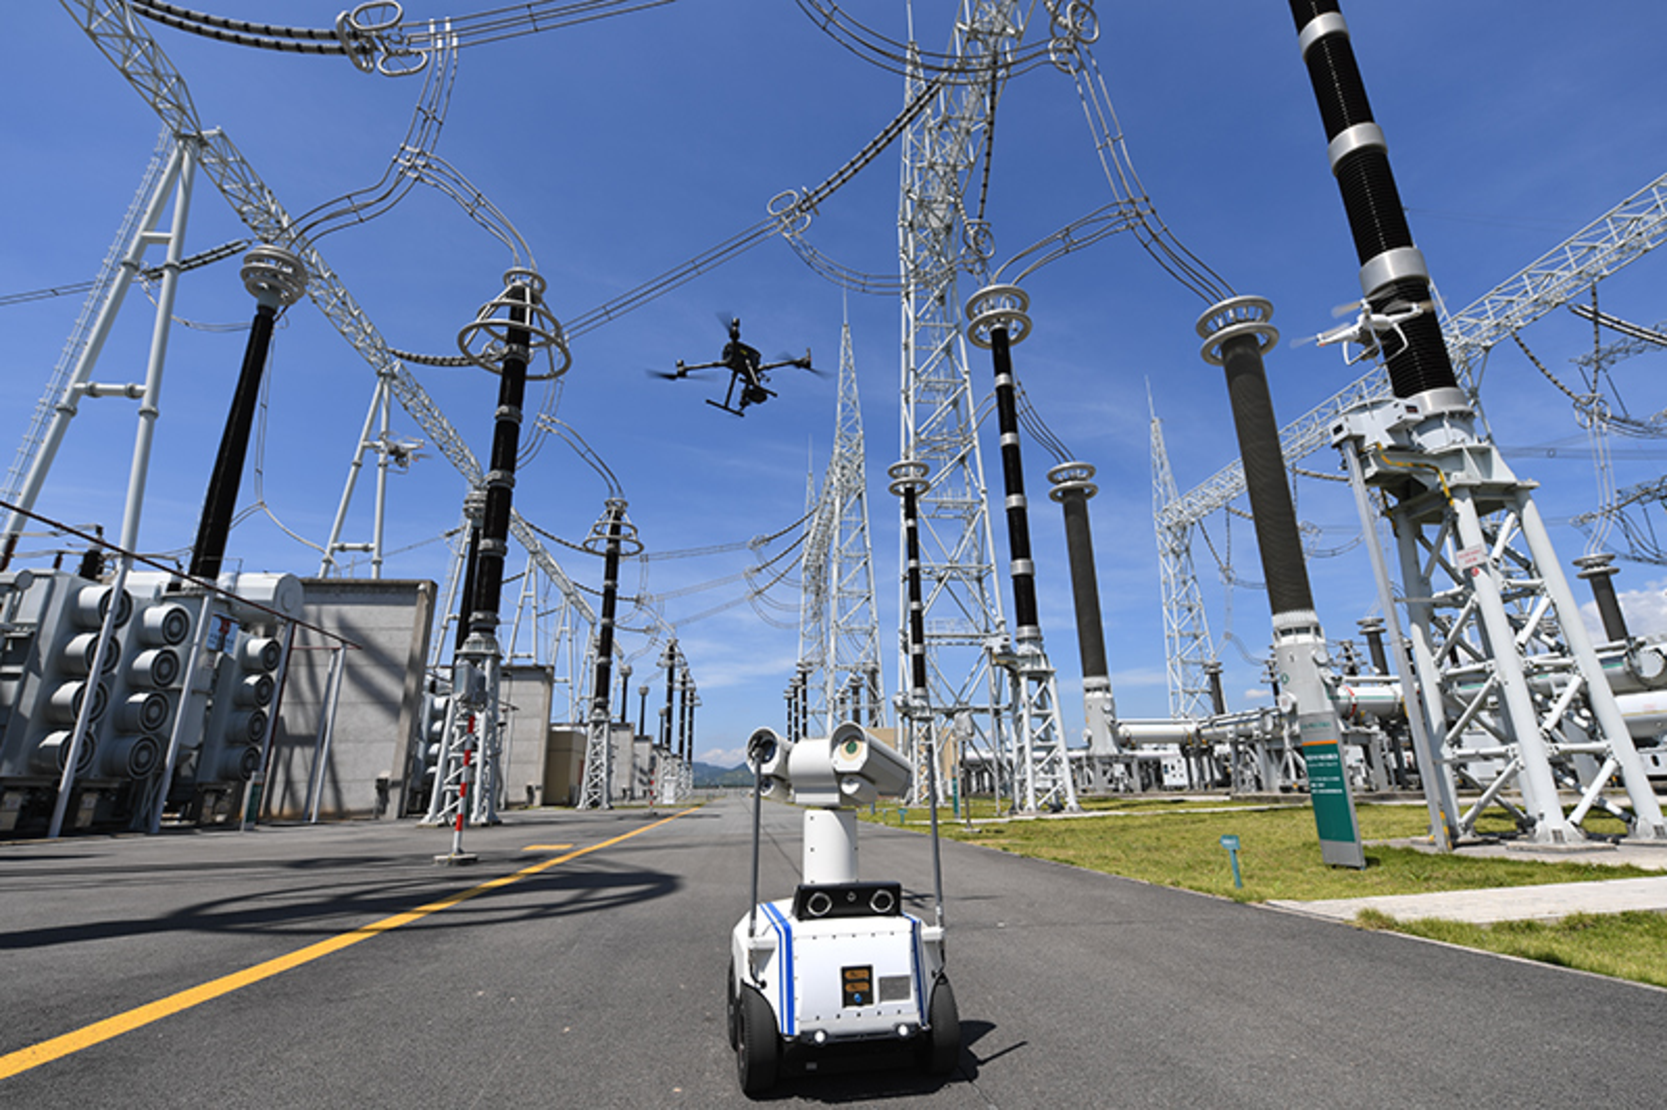
\includegraphics[width=\textwidth]{Apply3.pdf}
      \caption{变电站巡检车\cite{song2020xinhuawang}}
      \label{fig:apply_sub3}
  \end{subfigure}
  \begin{subfigure}[b]{0.45\textwidth}
      \centering
      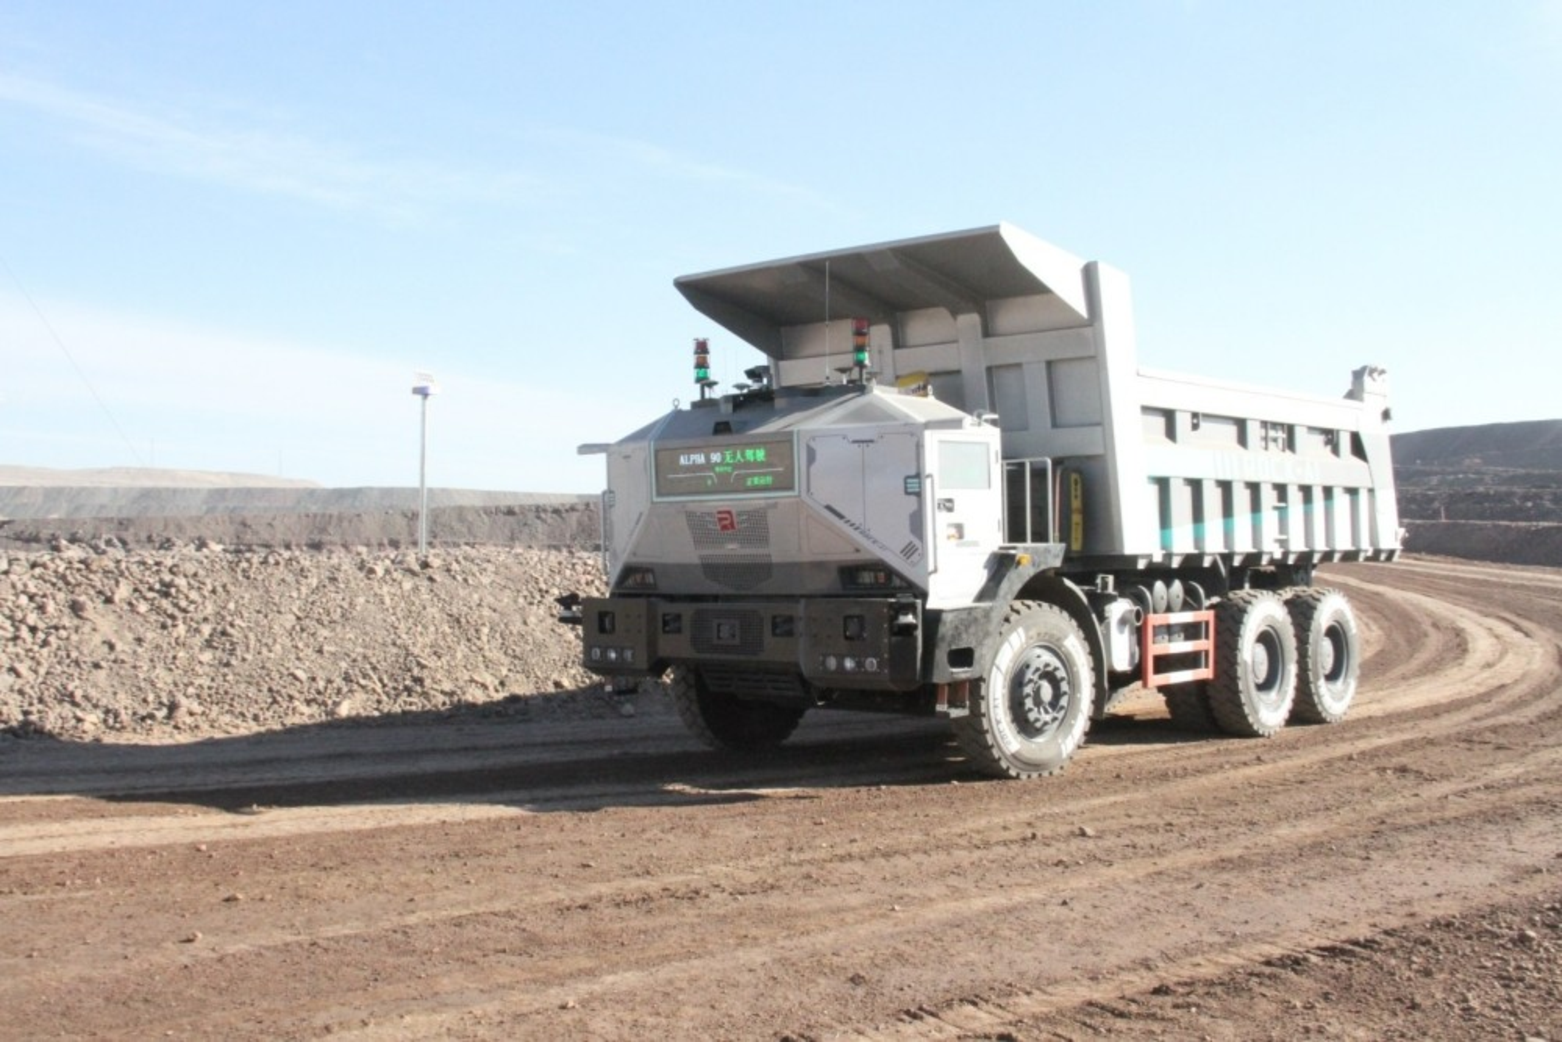
\includegraphics[width=\textwidth]{Apply4.pdf}
      \caption{矿山无人运输机器人\cite{li2023keji}}
      \label{fig:apply_sub4}
  \end{subfigure}

  \caption{固定路线定位的应用场景}
  \label{fig:apply}
\end{figure}

在定位方法中,视觉惯性定位(Visual-Inertial Localization)是一种应用广泛的定位形式,它通过融合视觉和惯性传感器的数据,实现对自身位置的估计。视觉传感器可以获取环境的视觉信息,而惯性传感器,例如惯性测量单元(Inertial Measurement Unit, IMU),可以获取自身的运动信息,两者结合可以实现对自身位置的估计。视觉惯性定位方法具有定位精度高、成本低、易于实现等优点,因此在固定路线定位中得到了广泛的应用。然而,视觉惯性定位方法也存在一些问题,例如视觉传感器易受光照、天气等环境因素影响,惯性传感器易受积分漂移等因素影响,这些因素都会影响视觉惯性定位的精度。因此,如何提高视觉惯性定位的精度,是当前固定路线定位研究的一个重要问题。

一种主要的改进方式是通过引入卫星导航系统(Global Navigation Satellite System, GNSS)信息来提高视觉惯性定位的精度。一般的商用低成本单频GNSS的精度在10米左右,这对于需要精确位置的智能化车辆和机器人来说是远远不够的。为了改进单频GNSS的精度,近年来出现了一些高精度的增强GNSS方法,例如精密单点定位(Precise Point Positioning, PPP)\cite{zumberge1997precise}技术和实时实时动态载波相位差分(Real Time Kinematic, RTK)\cite{fotopoulos2001overview}技术。PPP和RTK可以将GNSS的定位误差缩减至厘米级,是非常理想的高精度定位方法。但是PPP却因为需要较长的初始化时间\cite{bisnath2018innovation},所以不适合应用在实时定位场景上。而RTK虽然有不错的实时性,但是却经常容易受到天气、温度或者遮挡等问题的影响而产生单次误差较大的定位结果\cite{li2022review}。因此,直接引入GNSS观测信息会受到多种限制,并且高精度的GNSS服务也需要额外的费用,这对于一些低成本的固定路线定位系统来说是不可接受的。

另一种改进方式是通过引入地图信息来提高视觉惯性定位的精度。地图信息可以提供给视觉惯性定位系统一个先验的位置信息,从而可以减小定位误差。在固定路线条件下,由于车辆或机器人运行的路线是固定的,因此可以提前获取到路线的地图信息,这方便视觉惯性定位系统使用地图先验信息。除此之外,因为地图信息的收集过程并不受限于天气、温度等环境因素,而且没有实时性要求,可以在精心选择的条件下进行。因此,还可以融合高精度GNSS信息来提高建图精度。地图可以一次建立、多次使用,后续的使用成本相较于高精度GNSS服务要低廉得多。因此,引入地图信息是一种非常理想的提高视觉惯性定位精度的方法。

总的来说,固定路线中的视觉惯性定位是一项有着广泛应用的基础技术,但目前受限于视觉惯性定位技术本身的局限性,其精度还有待提高。在目前可选的改进方法中,引入地图信息是一种非常理想的提高视觉惯性定位精度的方法。因此,本文将围绕固定路线中的视觉惯性定位方法展开研究,通过解决地图构造、地图识别和地图使用等问题来提高定位的精度,为固定路线中的视觉惯性定位方法。


\section{研究意义}

(1) 以视觉惯性定位为基础,引入地图信息提高定位精度,是当下一种较为新颖的固定路线定位方法,本文将围绕这一方法展开研究,对提高固定路线中的智能汽车和机器人的定位精度具有理论意义。

(2)固定路线中的定位是自动驾驶和机器人领域中一项基础但重要的技术,本文针对这一技术开展研究,对提高固定路线中的智能汽车和机器人的定位精度具有实践意义。

(3)本文在地图的构建和使用中不仅有传统的空间计算、状态估计和非线性优化技术,还引入了基于深度学习的计算机视觉技术,对于推动传统定位技术和深度学习技术的融合具有一定的实践意义。


\section{国内外研究现状}
\subsection{视觉惯性定位}

视觉惯性定位是一种融合了视觉、惯性信息的定位方法,其中视觉信息一般来源于图像、视频等,而惯性信息则一般依靠IMU采集。视觉惯性定位方法以视觉定位和惯性定位技术为基础,但是目前的视觉惯性定位技术一般以视觉定位技术为核心,而惯性定位技术作为补充或约束信息加入到视觉定位中,因此介绍视觉惯性定位的发展有必要从视觉定位技术的发展说起。

% \subsubsection[short]{视觉定位方法}

\begin{figure}
  \centering
  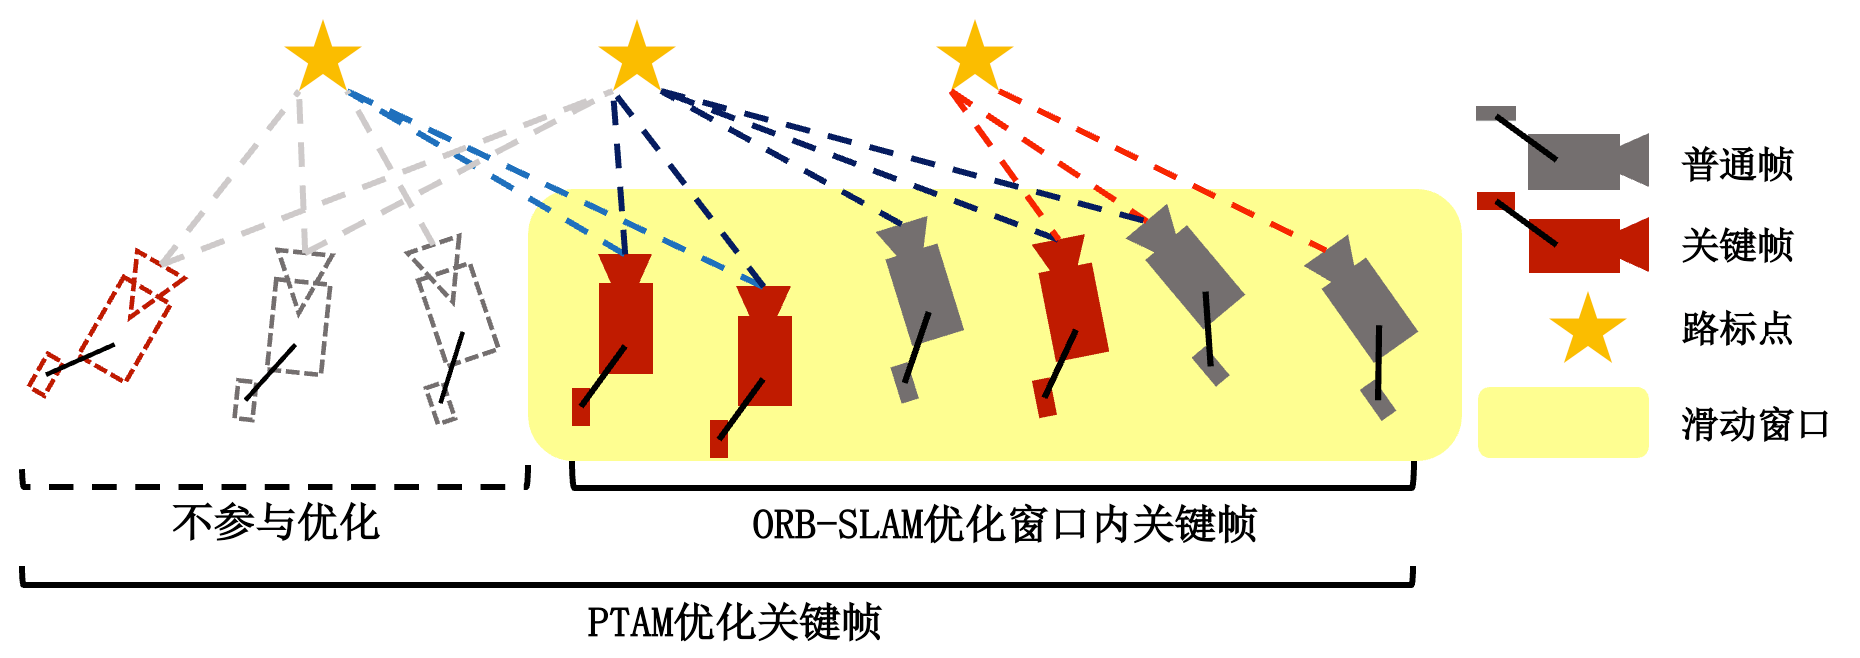
\includegraphics[width=0.9\linewidth]{vo_window.png}
  % \caption*{视觉定位中的关键帧和滑动窗口}
  \caption{视觉定位中的关键帧和滑动窗口}
  \label{fig:vo_window}
\end{figure}

视觉定位中常用的技术之一是同步定位与地图创建(Simultaneous Localization And Mapping, SLAM)。\citet{davison2007monoslam}于2007年首次提出了使用单目图像进行定位的方法MonoSLAM,以扩展卡尔曼滤波器(Extended Kalman Filter,EKF)为核心,实时对图像观测到的特征点进行位置估计,构建3D概率稀疏地图,然后使用地图点对相机位置和姿态进行估计,这是第一种能够达到实时的视觉定位方法,它使得利用视觉信息估计姿态成为可能。同年\citet{klein2007parallel}也提出了一种基于单目图像的定位方法PTAM(Parallel Tracking And Mapping) ,与MonoSLAM不同的是,PTAM的核心估计方法从扩展卡尔曼滤波器改变为光束法平差(Bundle Adjustment, BA)\cite{triggs2000bundle}。BA是一种非线性优化方法,其根据同一个地图点在多个图像上的观测位置,同时优化图像拍摄时相机的位姿和地图点的空间坐标。因为一次优化使用的数据更多,所以这种方法相比于滤波器更准确,但是计算量更大,所以PTAM引入了关键帧的概念:只对关键帧进行光束法平差,而对于普通帧则使用关键帧对其进行约束和定位估计。

PTAM 的另一大进步是将定位与建图两个功能解耦,使两个功能分别同时进行,而这一优点被\citet{mur2015orb,mur2017orb}吸取,创造出ORB-SLAM。ORB-SLAM是一个包含3个主要线程的完整SLAM系统:实时特征点跟踪(Tracking)线程、局部建图优化(Local Mapping)线程、回环检测(Loop Closing)线程。ORB-SLAM中不仅继承了PTAM的关键帧思想,还使用了如图\ref{fig:vo_window}所示的滑动窗口概念,进一步提高了系统实时性。滑动窗口设置包含固定数量关键帧的窗口,随着系统的工作,窗口随时添加新的关键帧并舍弃距离现在最远的关键帧,BA只优化当前窗口内关键帧及其地图点的信息。ORB-SLAM基本奠定了后来视觉定位方法的范式,其提出的3个功能模块也组成后续视觉定位方式的基本骨架。

虽然视觉定位的发展取得了一些进步,但是视觉定位的系统性缺陷却阻碍其应用。在视觉定位研究最广泛的单目视觉定位方面,其依靠的单目相机传感器天然缺少对深度的观测,这造成了单目视觉定位的尺度不确定性,即单目视觉定位不能获得真实世界尺度下的定位结果。为了解决这个问题,研究者们开始在视觉定位的基础上加入了可以获取真实世界尺度信息的传感器,例如惯性测量单元(Inertial measurement unit, IMU),提出了视觉惯性定位。

% \subsubsection{视觉惯性定位方法}
视觉惯性定位是视觉定位和惯性定位的结合,涉及到多传感器信息融合,根据融合方式可以分为松耦合\cite{lynen2013robust}与紧耦合\cite{falquez2016inertial}。松耦合方式是将视觉定位和惯性定位分开处理,让两种定位方式独立运行,然后对结果再进行融合,融合的方式可以选择扩展卡尔曼滤波或者非线性优化。松耦合的优点是系统简单,估计量少,因此不论是运行效率还是灵活度都非常高;缺点是忽略了两种定位方式之间的约束关系,所以精度较差。目前主流的视觉惯性定位基本是紧耦合方式,紧耦合需要将两种定位方式的估计量作为一个整体同时优化。

紧耦合视觉惯性定位方法最早以滤波器的形式发展,此时视觉惯性定位依旧是以IMU运动模型为核心,以线性化和观测性为主要研究方向,最突出的工作是\citet{mourikis2007multi}提出的多状态约束卡尔曼滤波(Multi-State Constraint Kalman Filter,MSCKF),该方法以IMU位置、姿态、速度等状态量和固定数量的相机位置、姿态为主要的估计参数,并没有将地图点加入到优化列表中。MSCKF工作的最主要贡献在于推导出一种测量模型,该模型能够表达从多个相机位姿观察到静态特征时出现的几何约束。

此后,许多基于MSCKF的工作相继提出,框架整体的精度和鲁棒性得到了不断的提升,例如\citet{li2013high}在MSCKF的基础上提出的MSCKF 2.0以及\citet{sun2018robust}提出的双目视觉版本MSCKF。\citet{bloesch2017iterated}提出了一种基于迭代扩展卡尔曼滤波器(Iterated extended Kalman filter,IEKF)的直接法单目视觉惯性里程计ROVIO(RObust Visual Inertial Odometry)。在视觉方面,该方法将地图点在图像中对应点周围的图像块作为路标点的描述子,从而得到光度误差,然后将光度误差进行变换得到IEKF中的启发项,进而进行滤波状态的更新。整体的滤波方程的构造是以IMU为中心进行构造的,保证能观状态不受不断增长的全局协方差的影响,这样可以减小因非线性而造成的误差。

\begin{figure}
  \centering
  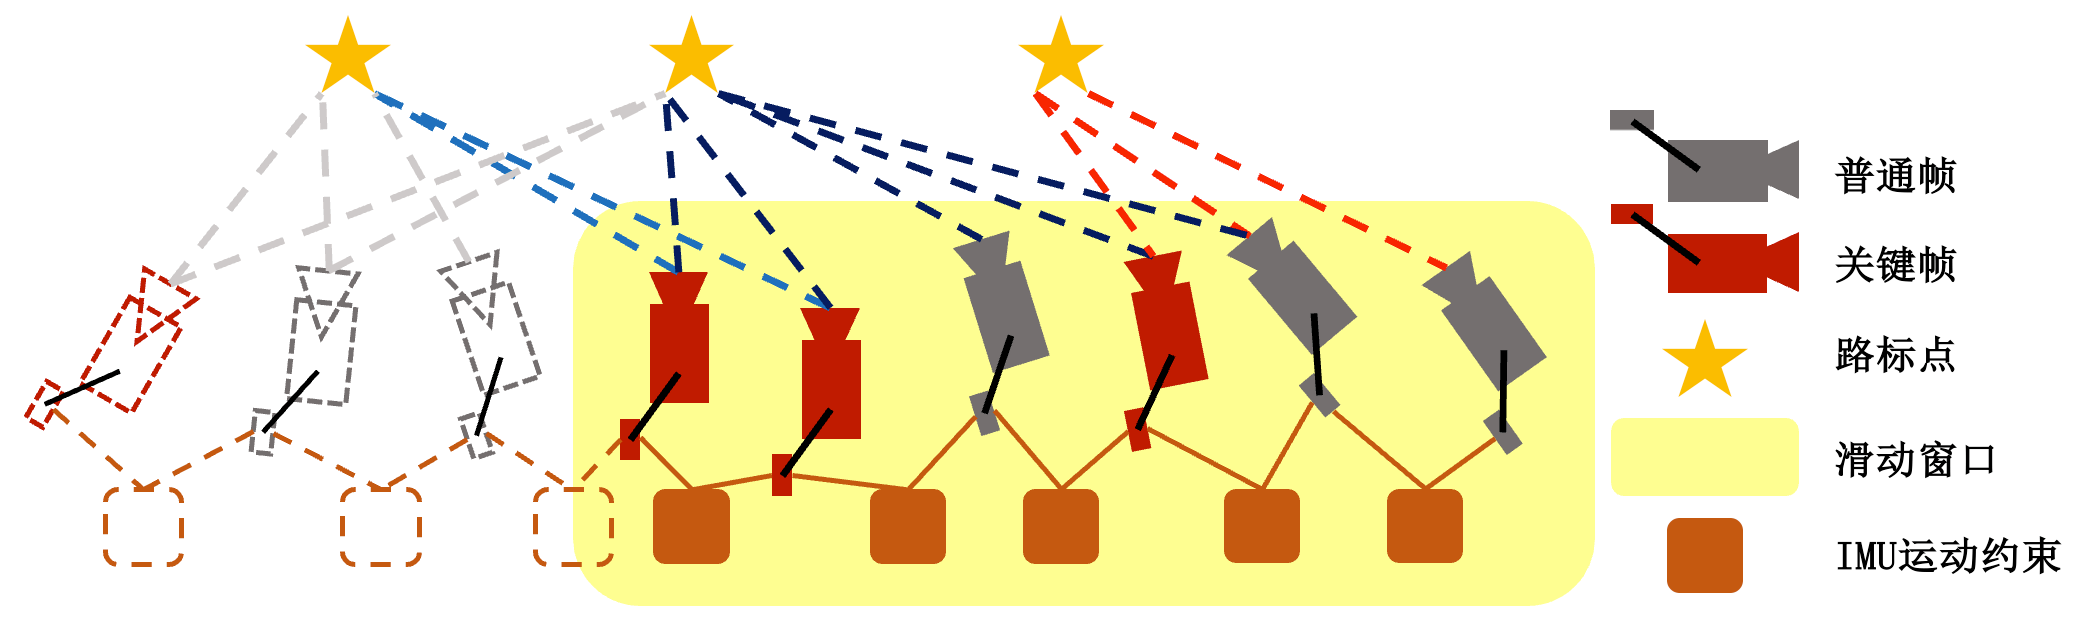
\includegraphics[width=1.0\linewidth]{vio_window.png}
  \caption{视觉惯性定位中的关键帧和滑动窗口}
  \label{fig:vio_window}
\end{figure}

近年来随着非线性优化在视觉定位中的广泛应用,视觉惯性定位方法也尝试使用这种优化方式。参考视觉定位中将地图点和相机位姿以图(Graph)的形式联系起来,然后使用光束法平差进行统一优化,视觉惯性定位在相机位姿之间加入由IMU数据组成的运动约束项,如图\ref{fig:vio_window}所示。IMU运动约束指的是IMU预积分,\citet{forster2016manifold}提出了应用于视觉惯性里程计中的基于四元数的预积分公式,将传统的IMU运动积分公式转化为帧间增量的形式,并且将运动积分中的IMU偏置(Bias)线性化,避免在优化过程中IMU偏置发生变化时重新积分,提高运行效率。\citet{leutenegger2015keyframe}提出的OKVIS(Open Keyframe-based Visual-Inertial SLAM)利用基于关键帧的滑动窗口进行批量非线性优化,先于滑动窗口的关键帧被边缘化,不用来进行估计。系统前端使用多尺度Harris\cite{harris1988combined}特征检测器来提取特征点,然后在其基础上计算BRISK(Binary Robust Invariant Scalable Keypoint)\cite{leutenegger2011brisk}描述子,以便在帧与帧之间进行数据关联。

\citet{qin2018vins}提出的VINS-Mono(Monocular Visual-INertial System)类似于OKVIS,但引入了几个全新的功能,其完整系统包括观测值预处理、初始化、局部视觉惯性联合优化、全局图优化和回环检测5个部分,前端提取Harri特征点,并采用LK光流(Lucas-Kanade opticalflow)\cite{lucas1981iterative}法跟踪相邻帧。VINS-Mono 方法只计算特征点,不计算描述子,同时使用光流法跟踪特征点的运动,这样就减少了计算和匹配描述子的时间和资源。系统采用与 OKVIS 相似的基于滑动窗口的紧耦合位姿估计方法,并且加入了基于词袋模型(Bag of Binary Words,DBoW)\cite{galvez2012bags}的回环检测线程,使系统具有重定位功能。\citet{liu2018ice}提出ICE-BA(Incremental, Consistent and Efficient Bundle Adjustment),沿用VINS-Mono中基于LK光流的特征点跟踪技术,后端则是提出了增量式BA,主要分为3个部分:局部BA、全局BA以及相对边缘化(Relative-Marginalization),前两者采用增量式方法提升了后端速度,后者保证了局部BA和全局BA的一致性。

一些视觉定位方法也发展出了融合惯性信息的版本,\citet{campos2021orb}在ORB-SLAM的基础上提出了ORB-SLAM 3,引入IMU尝试解决在快速运动时丢失特征点的问题:ORB-SLAM 3分别对ORB-SLAM的3个线程作出修改,用以融合IMU信息:在跟踪线程,基于重投影误差和IMU预积分,建立帧与帧之间的约束关系来构造代价函数,从而得到当前帧位姿的最优估计;在局部建图线程,有了新的关键帧之后,将会对前N个关键帧进行优化,当前的关键帧(第N+1帧)将固定不变;在全局回环检测线程,由于IMU提供了尺度信息,因此全局优化将从7个自由度下降到6个自由度,全局位姿优化将忽略IMU信息,因此不再优化速度和偏差,当完成全局位姿优化后,再根据矫正后的位姿对速度进行矫正。

\textbf{总结而言,视觉惯性定位系统的组成部分至今已基本定型,其主要由视觉SLAM系统的功能组件和预积分的惯性测量处理组成。因此,目前的视觉惯性定位方法仍遵循定位与建图同步的工作逻辑,并没有考虑过如何将先验地图运用到定位工作中。本文为了补充这一研究,希望提出一种地图辅助的视觉惯性定位方法,改变以往定位与建图高度同步的范式,这与此前的工作有较明显的差异。}

\subsection{地图辅助的定位方法}
地图辅助定位是一种车辆定位中常用的技术,常用的地图类型有高精(High-Definition,HD)地图、激光雷达点云地图、视觉重建地图等。\citet{jeong2020hdmi}开发了一种高效的HD地图表示方法,并利用粒子滤波器估计车辆的六自由度(6-Degree Of Freedom,DOF)位姿,该方法实现了分米级精度。\citet{xiao2020monocular}和Guo等人\cite{guo2021coarse}提出了一种基于HD地图的低成本视觉定位方法。这两种方法综合利用了低级地图特征(如点和线特征)以及结构特征(如地图元素的语义和类别),从而能够精确估计车辆的位姿。尽管上述方法在视觉定位方面取得了令人印象深刻的成果,但它们都依赖于成本高昂的高清地图,这些地图的构建需要细致的数据采集和人工标注。

为了降低对高清地图的依赖,研究者们开始探索基于图像和激光雷达扫描的地图构建方法。\citet{stewart2012laps}开发了一种利用单目相机在由搭载激光雷达传感器的测绘车辆预先生成的三维地图中进行定位的方法。该方法通过将激光雷达反射图像与图像强度进行匹配,并选择NMI(Normalized Mutual Information)最高的合成图像来确定相机位姿。\citet{zuo2019visual}采用基于MSCKF的视觉惯性里程计(Visual-Inertial Odometry, VIO)技术,在由激光雷达生成的点云地图中进行定位。具体而言,他们将点云地图作为观测值以更新MSCKF,从而提升其性能。\citet{lin2021autonomous}则将图像引入到先验地图信息中,其方法通过激光雷达估计位姿,同时利用车载图像构建稀疏点云地图。

近年来,随着视觉三维重建技术的进步,涌现了以SLAM和运动恢复结构(Structure from Motion,SfM)\cite{schonberger2016structure}为代表的地图重建方法。通过SLAM和SfM获得的重建地图一般包含地图关键帧的位姿、稀疏点云结构、稀疏点云特征等要素,这些要素可以在定位时快速提供粗略的位置参考,然后选择该位置附近的局部点云地图与当前定位图像进行细匹配和优化定位。具体来说,重建地图的地图关键帧的位姿可以通过特征点匹配、局部地图优化和全局地图优化等手段获得;重建地图的稀疏点云结构一般是通过提取地图关键帧的特征点,并根据地图关键帧的相对位姿三角化获得;重建地图的稀疏点云特征则是由地图关键帧的特征点描述子组成。在定位过程中,首先将待定位图像的特征点与地图的稀疏点云进行匹配,匹配到足够的地图点后可以使用PnP(Perspective-n-Point)算法直接计算待定位图像的位置和姿态。

在具体的重建地图使用方面,VINS-Mono、VINS-Fusion和ORB-SLAM 3等一些SLAM系统都已具有保存和加载先验地图的功能,这些SLAM系统可以提前在指定场景下初始运行、建图,而在此后的运行中依靠初始运行的结果进行定位。\citet{surber2017robust}提出了一种针对无人机的定位系统,旨在利用相机和IMU,在初始飞行中构建参考地图。在后续飞行中,系统通过VIO和图像匹配技术,将当前观测与参考地图进行对比,实现精确的自我定位。\citet{hao2023global}提出了一种两阶段的视觉惯性定位系统:在初始运行的过程中加入了额外的GNSS信息建图,而在后续运行中保持纯净的视觉惯性定位。在此系统中,初始运行阶段的GNSS信息提供了较强的位置约束,因此其所建地图精度得到了提升。这些地图使用方法思考了如何建立先验地图和实时场景中的特征点匹配关系,从而使用先验地图的精确地图点为当前定位提供参考。

然而,上述方法在匹配过程中依旧使用着传统的手工设计特征,这些特征在匹配精度和鲁棒性上仍有提升空间。除此之外,上述方法的重建地图基本都是基于SLAM系统的,这意味着地图的构建和定位是高度耦合的,系统本身的建图误差会传导、积累到定位过程中。虽然有工作\cite{hao2023global}尝试在建图阶段加入额外位置信息,提升建图效果,但其仍使用注重实时性的SLAM系统进行建图,依然会受到SLAM系统误差累积的影响。为了提升特征匹配的精度,同时降低建图误差对定位的影响,一些研究者开始尝试使用基于深度学习的特征搭配精度较高建图技术,例如SfM或者带GNSS增强的SfM\cite{vincentqin2022colmapgps},来提升整体的定位精度。

\citet{sarlin2019coarse}提出了一种“由粗到细”的地图使用方式:其建图过程使用SfM和具有精确位姿的图片进行;其定位方法首先使用基于深度学习的图片级描述子NetVLAD(Vector of Locally Aggregated Descriptors)\cite{arandjelovic2016netvlad}对定位图片进行粗位置查询,此后使用基于深度学习的像素级描述子SuperPoint\cite{detone2018superpoint}对定位图片的特征点进行细致匹配。这种方法在匹配过程中使用了基于深度学习的特征,从而提升了匹配的精度和鲁棒性,同时具有较高的实时性,为后续许多工作提供了一种地图定位范式。\citet{yang2022real}提出了一种基于视觉重建地图的定位方法,其方法在“由粗到细”定位的基础上引入了VIO,利用实际定位中的帧间相对位姿约束提升了定位精度。\citet{lin2023visual}则更是引入了多地图概念,其方法在匹配过程中使用了多个地图,从而提升了匹配的鲁棒性。

虽然这些方法在最终的定位精度上有所提升,但是存在一些问题。首先,这些研究在建图时直接假设地图图片的准确位姿是可获得的,这在实际操作中并不一定总是成立的。其次,这些研究聚焦于先验地图和实际定位之间的匹配关系,并尝试通过各种手段来增加匹配的约束,例如相对位姿、多地图验证等,但是却并没有考虑当地图和定位场景之间产生误匹配时如何降低误匹配的影响。这无疑导致了这些定位方法的脆弱性,使得他们在实际应用中表现出不稳定的性能。此外,\citet{yang2022real}在定位中引入了服务器组件,因此对通信环境的要求较高;\citet{lin2023visual}的方法使用多地图以及丰富的约束,导致运行过程内存占用极大(测试中使用4T RAM)。这些问题都限制了上述方法在实际应用中的推广。

\textbf{总结而言,地图辅助的定位方法研究较为分散,根据地图类型的不同,定位方法差异较大。使用HD地图和激光雷达点云地图的方法有较高精度,但是高昂的地图成本却也阻碍着这类技术在实际生产中的应用。基于重建地图的定位方式有较低的成本,但是当前的研究方法中还有一些限制,例如建图假设过强、定位容错不足和实际应用限制较多等问题。为了提供一种实施难度低、容错能力强、完全部署在汽车或机器人上的高精度定位方法,本文希望从建图方式开始,构建完整的固定路线中的视觉惯性定位系统,实现完全部署于车载或机器人端,并具有较高定位精度。}


\section{研究内容与创新}

本文的研究内容是提出一种完整固定路线视觉惯性定位方法,具体而言,本文将通过三个阶段的研究来逐步达成最终目标:(1)先验地图构建;(2)视觉与惯性信息的融合;(3)基于先验地图的位姿优化。


\textbf{(1)先验地图构建:}
辅助地图的构建是本文首先要解决的问题,是剩余其他研究内容的基础。因为SLAM类建图算法由于只进行局部优化,存在误差累积,精度较差的问题,所以本文采用SfM作为基础建图方法,其全局优化策略可以有效降低累计误差。虽然SfM建图具有理论精度高的优势,但原始的SfM建图不具备现实尺度。为了恢复出具有现实世界尺度的地图,必须增加有现实尺度的观测信息,本文所采用的观测信息为高精度GNSS,例如RTK信息。虽然RTK在使用时可能会存在瞬时测量受环境因素影响而产生波动等问题,但是对于建图环节来说,环境可以静心挑选,因此RTK完全可以运用在实际建图中,并且其较高精度的定位观测可以为建图优化提供较好的约束。

本文将着力于融合GNSS观测信息与SfM,提出一种精度较高且稳定性突出的视觉先验地图构建方式。所构建的地图将具有现实世界尺度,且地图关键帧具有较高的位姿估计精度。

\textbf{(2)视觉与惯性信息的融合:}
视觉信息和惯性信息的融合是定位的核心,决定着最终定位的精度如何。目前视觉惯性信息的融合方式主要分为卡尔曼滤波器和非线性优化两种,其中卡尔曼滤波器的优势是在估计矩阵维度较低时计算简单,速度较快,劣势是精度欠缺;非线性优化的方法能够提供较高的精度,且随着硬件技术进步,实时运行非线性优化方法也是可能的。

本文选择以非线性优化作为融合方案,着力于解决如何在非线性优化中构建视觉信息和惯性信息的约束关系,并加入符合固定路线运行的车辆和机器人的合理约束,提高融合后定位精度。

\textbf{(3)基于先验地图的位姿优化:}
在基于地图的定位方法中,建模先验地图在实际定位中的视觉观测,是将地图与定位结合起来的关键。先验地图的视觉观测首先要解决的问题是将地图点与待定位图像特征点进行关联,构建图像特征点观测与图像位置、姿态参数之间的转换关系。基于特征点和描述子的关联方式具有一定的可行性,但是考虑到建图过程可能与实际定位过程有较大的场景表现差异,需要选择对场景差异不敏感的特征点及描述子。除了选择特征点与描述子,基于先验地图稀疏点云的位姿优化也直接关系到定位的精度。先验建图过程中产生的稀疏点云结构,其自身所在的坐标系可能与实际定位时的坐标系并不一致,如何对其坐标系对齐,以及对齐后如何使用先验点云结构来优化实际定位的位姿,是需要解决的问题。

本文将着力于使用一种基于数据驱动的,能够对场景差异较为鲁棒的先验地图视觉观测技术,构建定位与先验建图的关联。在这一基础上提出一种能够对齐先验地图坐标系和实际定位坐标系,以及一种先验地图的合理使用方式来融合先验信息和当下观测,以获得高精度定位结果。

本文的创新点主要体现在以下几个方面:

(1)提出了一种新颖且完整的固定路线视觉惯性定位方法,该方法将先验地图构建、视觉与惯性信息融合、基于先验地图的位姿优化三个阶段有机结合,形成一个完整的视觉惯性定位系统。

(2)在先验地图构建阶段,本文将采用SfM和高精度GNSS观测数据相结合的方式,构建具有现实世界尺度的多层次先验地图,提高地图的精度和稳定性。

(3)在视觉与惯性信息融合阶段,本文提出了一种基于车身运动学约束的视觉惯性里程计,该视觉里程计使用深度神经网络对车身状态进行检测,针对直行状态下的车辆或轮式机器人进行速度观测约束,提高了里程计的估计精度。

(4)在基于先验地图的位姿优化阶段,本文将提出一种新的基于先验地图的位姿优化方法,该方法使用基于深度学习的粗到细定位等手段获得基于先验地图的视觉观测,同时将先验地图的点云结构建模为高斯概率地图,以最大后验概率估计的方式完成位姿优化。

\section{论文组织结构}
本文共六章,各章内容安排如下:

第一章为绪论,首先介绍了本文的研究背景、研究意义,此后根据对国内外研究的调研介绍相关研究进展,通过与现有研究的对比引出本文研究的侧重点,并概括本文的研究内容,最后对全文结构进行介绍。

第二章为系统介绍,首先对整个系统的框架进行了展示,对其中3个主要模块,即离线建图模块、视觉惯性里程计模块和紧耦合地图定位模块进行了详细介绍,分别明确了他们的输出输出已经信息交互关系;此后介绍了该系统中所设计的所有坐标系,为后文统一描述各个模块的内部组成提供了基础;在这之后介绍了离线建图模块的基本过程,包括建图预处理、SfM、建图对齐和建图融合等过程,对每个过程的内部原理做出详细解释;最终介绍了建图模块的输出,即粗细两个粒度的层次先验地图。

第三章为视觉惯性里程计模块介绍,首先从车身运动的情况分类入手,介绍了本文中对于车身状态的三种假设,即静止、直行和转弯;此后介绍了一种以深度学习为基础的车身状态检测方法,该方法使用Transformer网络对惯性信息序列进行分类,以检测车辆处于何种状态;在这之后介绍了一种车身坐标系和IMU体坐标系之间的转换方法,其可以粗略估计两个坐标系的关系;最后介绍了如何将车身状态假设融合到视觉惯性里程计后端优化中,给出了基于车身状态的速度观测约束并求解相关的雅可比矩阵,使得位姿估计问题可以被非线性优化求解。

第四章为紧耦合地图定位模块介绍,首先介绍了基于深度学习的描述子在视觉观测中的优势,由此介绍基于深度学习的粗到细定位方法;此后介绍了转换矩阵初始化和有效性验证,这两部分共同工作,能够完成从视觉惯性里程计定位和粗到细定位的统一,使得多源的定位观测未来可以在统一坐标系下使用;在这之后是紧耦合优化介绍,这一部分详细推导了如何将先验地图建模为高斯概率地图,以及如何以非线性优化的形式完成最大后验概率估计;最后介绍了转换矩阵的更新,论述了其必要性以及详细的转化方法。

第五章为实验与结果分析,首先对实验实施的环境、参数和数据集等信息进行了介绍;此后分别针对本文提出的3个模块进行实验,再对整个系统的性能进行了综合评估,并对实验结果进行了详细的分析,分别从定位精度、定位鲁棒性、定位实时性等方面进行了评估;最后进行了消融实验,更加细致得验证了本文提出的方法的有效性。

第六章为总结与展望,首先总结了本文的研究工作,然后对本文的研究工作进行了展望,提出了未来的改进方向。
% !TeX root = ../thuthesis-example.tex

\chapter{系统框架与离线建图}

\section{系统框架}

本文所提出方法的整体设计如图\ref{fig:overall}所示,其主要包括两个阶段:建图和定位。在建图阶段,离线建图模块使用图片和高精度GNSS信息构建包含粗粒度和细粒度信息的先验地图。在定位阶段又可以分为两个模块:视觉惯性里程计模块和紧耦合地图定位模块。

视觉惯性里程计使用图片和惯性信息可以获得连续图片的相对位姿变换;紧耦合地图定位则VIO结果和地图观测完成最后的定位,获得相机位姿。整个系统的设计与研究内容的对应关系是:离线建图模块对应着先验地图构建的研究内容,将在本章着重介绍;VIO对应着视觉与惯性信息的融合的研究内容,将在第3章中着重介绍;紧耦合地图定位对应着基于先验地图的位姿优化的研究内容,将在第4章中着重介绍。

\begin{figure}
  \centering
  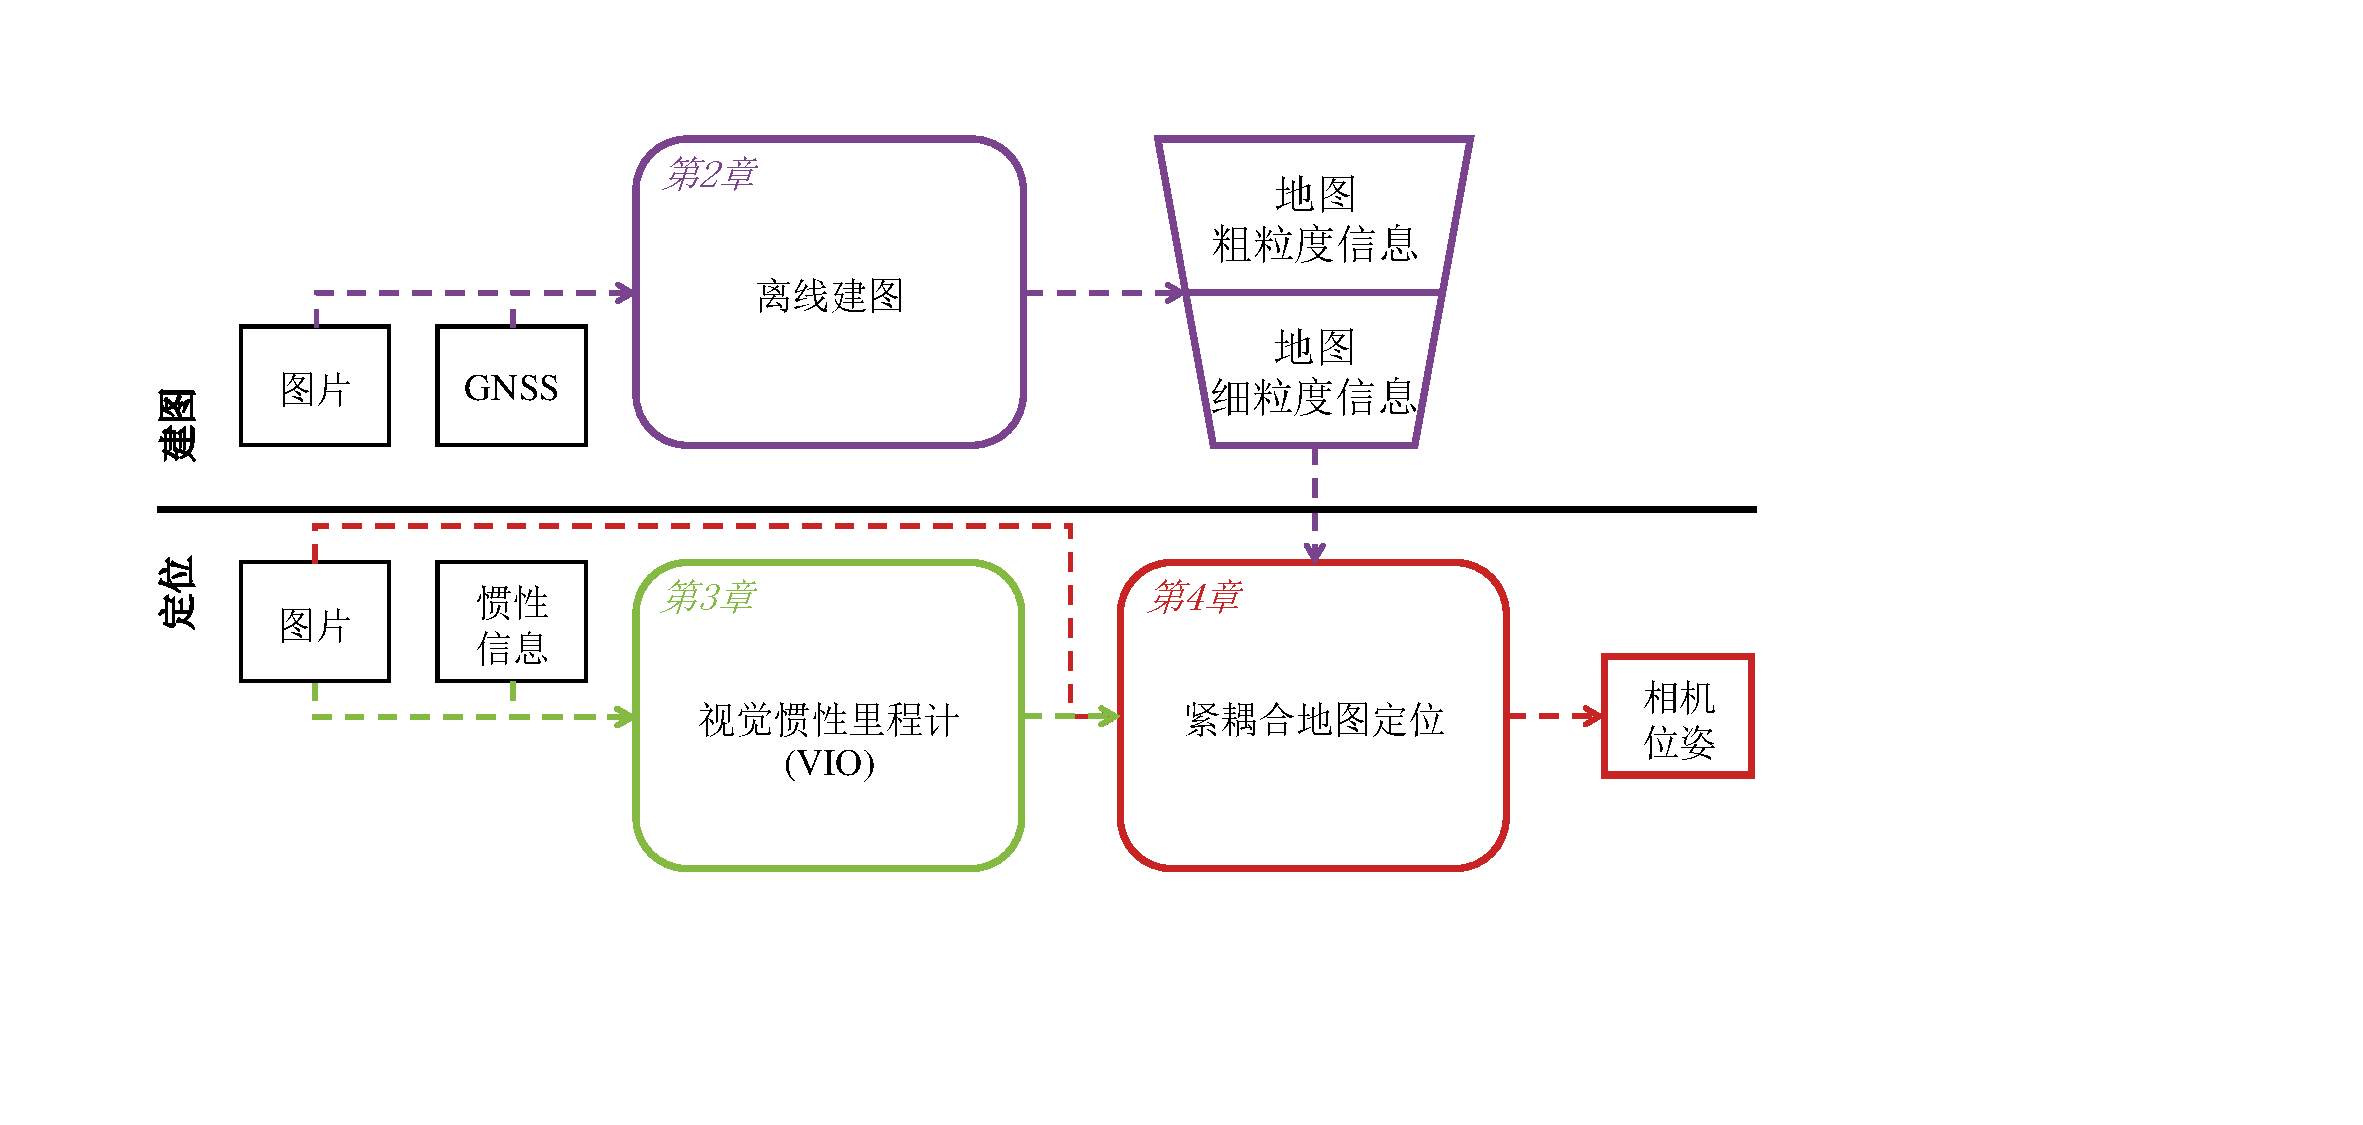
\includegraphics[width=1.0\linewidth]{overall.pdf}
  \caption{系统框架的设计示意图}
  \label{fig:overall}
\end{figure}

建图阶段,离线建图模块利用GNSS观测数据和图像构建一个包含粗粒度层级和细粒度层级组成的分层先验地图。粗粒度层级包括地图关键帧的位姿和关键帧描述子,而细粒度层级则包含稀疏点云结构及点云点描述子。添加GNSS观测的SfM是离线建图模块的核心,使用这一技术有以下的必要性:首先,SfM作为一种具有全局优化功能的建图方式,其相较于SLAM更适合建立高精度的地图;其次,SfM作为一种单目建图技术,其所创建的地图并不具有真实物理世界的尺度,因此必须添加具有尺度信息的GNSS信息作为补充,以获得具有真实世界尺度的地图;最后,相对精确的GNSS信息对于SfM的建图过程也有增益,有助于获得更加精确的地图。

基于建图阶段所构建的分层先验地图,视觉惯性里程计模块和紧耦合地图定位模块计算实际定位时所拍摄图像在全局坐标系中的位姿。

在视觉惯性里程计模块中,图像和惯性信息经过融合后可以相对精确地估算相邻图片之间的位姿变换,虽然这种相对信息虽然不是绝对的全局位姿,不可以直接用来作为定位结果,但是可以作为约束条件用于实际的地图定位。作为一种约束条件,视觉惯性里程计的精度对于整个定位系统的性能也发挥着重要作用,因此,本文将提升视觉里程计的精度也作为一项重要研究内容。

紧耦合定位模块是整个系统最后,也是最重要的模块,其主要功能包括地图观测与定位、视觉惯性里程计对齐、紧耦合位姿优化等。地图的观测与定位将实际拍摄的图片与地图进行粗到细匹配,逐渐获得一个较为粗糙的位姿观测;视觉惯性里程计对齐则将视觉惯性里程计的相对位姿转化到地图坐标系中,方便其后续使用;紧耦合位姿优化是整个模块的核心,其同时参考视觉惯性里程计、地图观测以及地图先验信息,通过非线性优化算法获得最终的精确位姿。

\begin{figure}
  \centering
  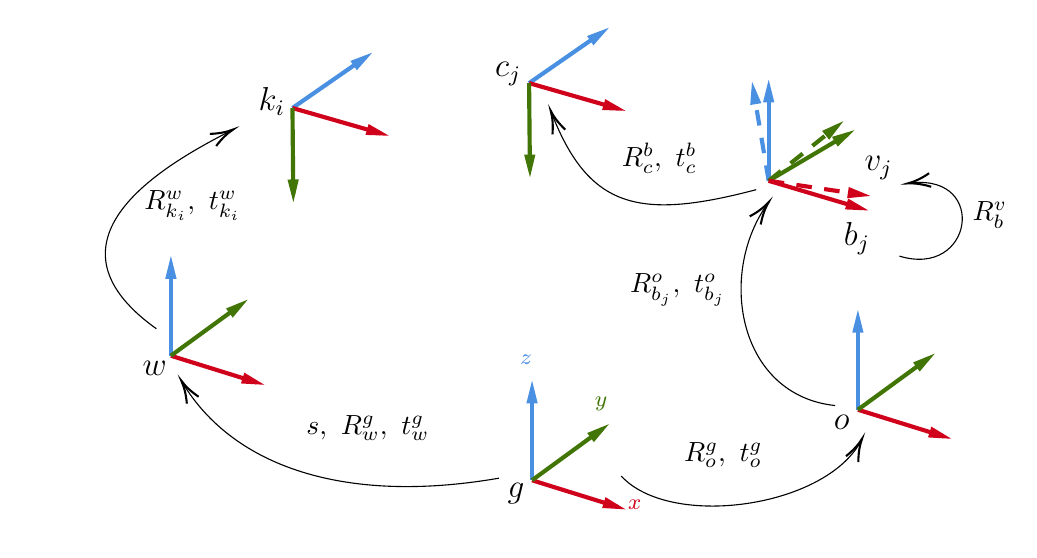
\begin{tikzpicture}[x=0.75pt,y=0.75pt,yscale=-1,xscale=1]
    %uncomment if require: \path (0,381); %set diagram left start at 0, and has height of 381
    
    %Straight Lines [id:da010349331460429267] 
    \draw [color={rgb, 255:red, 74; green, 144; blue, 226 }  ,draw opacity=1 ][line width=1.5]    (405,86.72) -- (405,42) ;
    \draw [shift={(405,38)}, rotate = 90] [fill={rgb, 255:red, 74; green, 144; blue, 226 }  ,fill opacity=1 ][line width=0.08]  [draw opacity=0] (10.92,-2.73) -- (0,0) -- (10.92,2.73) -- cycle    ;
    %Straight Lines [id:da02660288208799133] 
    \draw [color={rgb, 255:red, 208; green, 2; blue, 27 }  ,draw opacity=1 ][line width=1.5]    (405,86.72) -- (449.17,99.86) ;
    \draw [shift={(453,101)}, rotate = 196.57] [fill={rgb, 255:red, 208; green, 2; blue, 27 }  ,fill opacity=1 ][line width=0.08]  [draw opacity=0] (10.92,-2.73) -- (0,0) -- (10.92,2.73) -- cycle    ;
    %Straight Lines [id:da6739104782471683] 
    \draw [color={rgb, 255:red, 65; green, 117; blue, 5 }  ,draw opacity=1 ][line width=1.5]    (405,86.72) -- (442.86,64.39) ;
    \draw [shift={(446.3,62.36)}, rotate = 149.47] [fill={rgb, 255:red, 65; green, 117; blue, 5 }  ,fill opacity=1 ][line width=0.08]  [draw opacity=0] (10.92,-2.73) -- (0,0) -- (10.92,2.73) -- cycle    ;
    %Straight Lines [id:da8429448182305654] 
    \draw [color={rgb, 255:red, 74; green, 144; blue, 226 }  ,draw opacity=1 ][line width=1.5]  [dash pattern={on 5.63pt off 4.5pt}]  (405,86.72) -- (397.66,42.94) ;
    \draw [shift={(397,39)}, rotate = 80.48] [fill={rgb, 255:red, 74; green, 144; blue, 226 }  ,fill opacity=1 ][line width=0.08]  [draw opacity=0] (10.92,-2.73) -- (0,0) -- (10.92,2.73) -- cycle    ;
    %Straight Lines [id:da4153681450236333] 
    \draw [color={rgb, 255:red, 65; green, 117; blue, 5 }  ,draw opacity=1 ][line width=1.5]  [dash pattern={on 5.63pt off 4.5pt}]  (405,86.72) -- (437.87,60.49) ;
    \draw [shift={(441,58)}, rotate = 141.42] [fill={rgb, 255:red, 65; green, 117; blue, 5 }  ,fill opacity=1 ][line width=0.08]  [draw opacity=0] (10.92,-2.73) -- (0,0) -- (10.92,2.73) -- cycle    ;
    %Straight Lines [id:da43505559959247075] 
    \draw [color={rgb, 255:red, 208; green, 2; blue, 27 }  ,draw opacity=1 ][line width=1.5]  [dash pattern={on 5.63pt off 4.5pt}]  (405,86.72) -- (450.04,93.41) ;
    \draw [shift={(454,94)}, rotate = 188.45] [fill={rgb, 255:red, 208; green, 2; blue, 27 }  ,fill opacity=1 ][line width=0.08]  [draw opacity=0] (10.92,-2.73) -- (0,0) -- (10.92,2.73) -- cycle    ;
    %Straight Lines [id:da48780320413370326] 
    \draw [color={rgb, 255:red, 74; green, 144; blue, 226 }  ,draw opacity=1 ][line width=1.5]    (289.57,39.65) -- (324.71,15.28) ;
    \draw [shift={(328,13)}, rotate = 145.26] [fill={rgb, 255:red, 74; green, 144; blue, 226 }  ,fill opacity=1 ][line width=0.08]  [draw opacity=0] (10.92,-2.73) -- (0,0) -- (10.92,2.73) -- cycle    ;
    %Straight Lines [id:da6562561044670461] 
    \draw [color={rgb, 255:red, 208; green, 2; blue, 27 }  ,draw opacity=1 ][line width=1.5]    (289.57,39.65) -- (332.16,51.89) ;
    \draw [shift={(336,53)}, rotate = 196.04] [fill={rgb, 255:red, 208; green, 2; blue, 27 }  ,fill opacity=1 ][line width=0.08]  [draw opacity=0] (10.92,-2.73) -- (0,0) -- (10.92,2.73) -- cycle    ;
    %Straight Lines [id:da9240801597191248] 
    \draw [color={rgb, 255:red, 65; green, 117; blue, 5 }  ,draw opacity=1 ][line width=1.5]    (289.57,39.65) -- (289.96,81) ;
    \draw [shift={(290,85)}, rotate = 269.46] [fill={rgb, 255:red, 65; green, 117; blue, 5 }  ,fill opacity=1 ][line width=0.08]  [draw opacity=0] (10.92,-2.73) -- (0,0) -- (10.92,2.73) -- cycle    ;
    %Straight Lines [id:da4201279280840913] 
    \draw [color={rgb, 255:red, 74; green, 144; blue, 226 }  ,draw opacity=1 ][line width=1.5]    (291,231) -- (291,187) ;
    \draw [shift={(291,183)}, rotate = 90] [fill={rgb, 255:red, 74; green, 144; blue, 226 }  ,fill opacity=1 ][line width=0.08]  [draw opacity=0] (10.92,-2.73) -- (0,0) -- (10.92,2.73) -- cycle    ;
    %Straight Lines [id:da6007126321346508] 
    \draw [color={rgb, 255:red, 208; green, 2; blue, 27 }  ,draw opacity=1 ][line width=1.5]    (291,231) -- (332.18,243.81) ;
    \draw [shift={(336,245)}, rotate = 197.28] [fill={rgb, 255:red, 208; green, 2; blue, 27 }  ,fill opacity=1 ][line width=0.08]  [draw opacity=0] (10.92,-2.73) -- (0,0) -- (10.92,2.73) -- cycle    ;
    %Straight Lines [id:da330854614248709] 
    \draw [color={rgb, 255:red, 65; green, 117; blue, 5 }  ,draw opacity=1 ][line width=1.5]    (291,231) -- (324.77,206.36) ;
    \draw [shift={(328,204)}, rotate = 143.88] [fill={rgb, 255:red, 65; green, 117; blue, 5 }  ,fill opacity=1 ][line width=0.08]  [draw opacity=0] (10.92,-2.73) -- (0,0) -- (10.92,2.73) -- cycle    ;
    %Straight Lines [id:da595243483227706] 
    \draw [color={rgb, 255:red, 74; green, 144; blue, 226 }  ,draw opacity=1 ][line width=1.5]    (175.57,51.65) -- (210.71,27.28) ;
    \draw [shift={(214,25)}, rotate = 145.26] [fill={rgb, 255:red, 74; green, 144; blue, 226 }  ,fill opacity=1 ][line width=0.08]  [draw opacity=0] (10.92,-2.73) -- (0,0) -- (10.92,2.73) -- cycle    ;
    %Straight Lines [id:da0027345710245019195] 
    \draw [color={rgb, 255:red, 208; green, 2; blue, 27 }  ,draw opacity=1 ][line width=1.5]    (175.57,51.65) -- (218.16,63.89) ;
    \draw [shift={(222,65)}, rotate = 196.04] [fill={rgb, 255:red, 208; green, 2; blue, 27 }  ,fill opacity=1 ][line width=0.08]  [draw opacity=0] (10.92,-2.73) -- (0,0) -- (10.92,2.73) -- cycle    ;
    %Straight Lines [id:da21368714347529183] 
    \draw [color={rgb, 255:red, 65; green, 117; blue, 5 }  ,draw opacity=1 ][line width=1.5]    (175.57,51.65) -- (175.96,93) ;
    \draw [shift={(176,97)}, rotate = 269.46] [fill={rgb, 255:red, 65; green, 117; blue, 5 }  ,fill opacity=1 ][line width=0.08]  [draw opacity=0] (10.92,-2.73) -- (0,0) -- (10.92,2.73) -- cycle    ;
    %Curve Lines [id:da1757347987273996] 
    \draw    (275,230) .. controls (200.75,242.87) and (147.08,224.38) .. (122.73,184.22) ;
    \draw [shift={(122,183)}, rotate = 59.66] [color={rgb, 255:red, 0; green, 0; blue, 0 }  ][line width=0.75]    (10.93,-3.29) .. controls (6.95,-1.4) and (3.31,-0.3) .. (0,0) .. controls (3.31,0.3) and (6.95,1.4) .. (10.93,3.29)   ;
    %Curve Lines [id:da3602253572900054] 
    \draw    (437,195) .. controls (390.71,190.08) and (380.31,132.76) .. (403.9,98.55) ;
    \draw [shift={(405,97)}, rotate = 126.33] [color={rgb, 255:red, 0; green, 0; blue, 0 }  ][line width=0.75]    (10.93,-3.29) .. controls (6.95,-1.4) and (3.31,-0.3) .. (0,0) .. controls (3.31,0.3) and (6.95,1.4) .. (10.93,3.29)   ;
    %Curve Lines [id:da717594302866559] 
    \draw    (399,91) .. controls (342.57,105.85) and (318.48,100.12) .. (300.54,54.4) ;
    \draw [shift={(300,53)}, rotate = 69.04] [color={rgb, 255:red, 0; green, 0; blue, 0 }  ][line width=0.75]    (10.93,-3.29) .. controls (6.95,-1.4) and (3.31,-0.3) .. (0,0) .. controls (3.31,0.3) and (6.95,1.4) .. (10.93,3.29)   ;
    %Curve Lines [id:da9528892708598942] 
    \draw    (474.28,87.71) .. controls (510.71,84.05) and (503.28,133.78) .. (468,123) ;
    \draw [shift={(472,88)}, rotate = 351.25] [color={rgb, 255:red, 0; green, 0; blue, 0 }  ][line width=0.75]    (10.93,-3.29) .. controls (6.95,-1.4) and (3.31,-0.3) .. (0,0) .. controls (3.31,0.3) and (6.95,1.4) .. (10.93,3.29)   ;
    %Straight Lines [id:da32735696638940537] 
    \draw [color={rgb, 255:red, 74; green, 144; blue, 226 }  ,draw opacity=1 ][line width=1.5]    (117,171) -- (117,127) ;
    \draw [shift={(117,123)}, rotate = 90] [fill={rgb, 255:red, 74; green, 144; blue, 226 }  ,fill opacity=1 ][line width=0.08]  [draw opacity=0] (10.92,-2.73) -- (0,0) -- (10.92,2.73) -- cycle    ;
    %Straight Lines [id:da3558357238587271] 
    \draw [color={rgb, 255:red, 208; green, 2; blue, 27 }  ,draw opacity=1 ][line width=1.5]    (117,171) -- (158.18,183.81) ;
    \draw [shift={(162,185)}, rotate = 197.28] [fill={rgb, 255:red, 208; green, 2; blue, 27 }  ,fill opacity=1 ][line width=0.08]  [draw opacity=0] (10.92,-2.73) -- (0,0) -- (10.92,2.73) -- cycle    ;
    %Straight Lines [id:da2766511803624683] 
    \draw [color={rgb, 255:red, 65; green, 117; blue, 5 }  ,draw opacity=1 ][line width=1.5]    (117,171) -- (150.77,146.36) ;
    \draw [shift={(154,144)}, rotate = 143.88] [fill={rgb, 255:red, 65; green, 117; blue, 5 }  ,fill opacity=1 ][line width=0.08]  [draw opacity=0] (10.92,-2.73) -- (0,0) -- (10.92,2.73) -- cycle    ;
    %Curve Lines [id:da33324184111748867] 
    \draw    (110,158) .. controls (48.26,113.9) and (119.06,76.52) .. (145.44,62.81) ;
    \draw [shift={(147,62)}, rotate = 152.53] [color={rgb, 255:red, 0; green, 0; blue, 0 }  ][line width=0.75]    (10.93,-3.29) .. controls (6.95,-1.4) and (3.31,-0.3) .. (0,0) .. controls (3.31,0.3) and (6.95,1.4) .. (10.93,3.29)   ;
    %Straight Lines [id:da36807520055181286] 
    \draw [color={rgb, 255:red, 74; green, 144; blue, 226 }  ,draw opacity=1 ][line width=1.5]    (448,197) -- (448,153) ;
    \draw [shift={(448,149)}, rotate = 90] [fill={rgb, 255:red, 74; green, 144; blue, 226 }  ,fill opacity=1 ][line width=0.08]  [draw opacity=0] (10.92,-2.73) -- (0,0) -- (10.92,2.73) -- cycle    ;
    %Straight Lines [id:da4244155612226017] 
    \draw [color={rgb, 255:red, 208; green, 2; blue, 27 }  ,draw opacity=1 ][line width=1.5]    (448,197) -- (489.18,209.81) ;
    \draw [shift={(493,211)}, rotate = 197.28] [fill={rgb, 255:red, 208; green, 2; blue, 27 }  ,fill opacity=1 ][line width=0.08]  [draw opacity=0] (10.92,-2.73) -- (0,0) -- (10.92,2.73) -- cycle    ;
    %Straight Lines [id:da45355668966659435] 
    \draw [color={rgb, 255:red, 65; green, 117; blue, 5 }  ,draw opacity=1 ][line width=1.5]    (448,197) -- (481.77,172.36) ;
    \draw [shift={(485,170)}, rotate = 143.88] [fill={rgb, 255:red, 65; green, 117; blue, 5 }  ,fill opacity=1 ][line width=0.08]  [draw opacity=0] (10.92,-2.73) -- (0,0) -- (10.92,2.73) -- cycle    ;
    %Curve Lines [id:da4763366607897037] 
    \draw    (334,229) .. controls (357.64,254.61) and (431.73,244.32) .. (449.24,212.47) ;
    \draw [shift={(450,211)}, rotate = 115.87] [color={rgb, 255:red, 0; green, 0; blue, 0 }  ][line width=0.75]    (10.93,-3.29) .. controls (6.95,-1.4) and (3.31,-0.3) .. (0,0) .. controls (3.31,0.3) and (6.95,1.4) .. (10.93,3.29)   ;
    
    % Text Node
    \draw (440,105.4) node [anchor=north west][inner sep=0.75pt]  [font=\large]  {$b_{j}$};
    % Text Node
    \draw (450,73.4) node [anchor=north west][inner sep=0.75pt]  [font=\large]  {$v_{j}$};
    % Text Node
    \draw (272,28.4) node [anchor=north west][inner sep=0.75pt]  [font=\large]  {$c_{j}$};
    % Text Node
    \draw (283.22,237.24) node  [font=\large]  {$\mathnormal{g}$};
    % Text Node
    \draw (158,40.4) node [anchor=north west][inner sep=0.75pt]  [font=\large]  {$k_{i}$};
    % Text Node
    \draw (181,198.4) node [anchor=north west][inner sep=0.75pt]    {$\mathnormal{s} ,\ \boldsymbol{R}_{w}^{g} ,\ t_{w}^{g}$};
    % Text Node
    \draw (337,130.4) node [anchor=north west][inner sep=0.75pt]    {$\boldsymbol{R}_{b_{j}}^{o} ,\ t_{b_{j}}^{o}$};
    % Text Node
    \draw (333,67.4) node [anchor=north west][inner sep=0.75pt]    {$\boldsymbol{R}_{c}^{b} ,\ t_{c}^{b}$};
    % Text Node
    \draw (502,95.4) node [anchor=north west][inner sep=0.75pt]    {$\boldsymbol{R}_{b}^{v}$};
    % Text Node
    \draw (109.22,177.24) node  [font=\large]  {$w$};
    % Text Node
    \draw (103,90.4) node [anchor=north west][inner sep=0.75pt]    {$\boldsymbol{R}_{k_{i}}^{w} ,\ t_{k_{i}}^{w}$};
    % Text Node
    \draw (336,239.4) node [anchor=north west][inner sep=0.75pt]  [font=\footnotesize,color={rgb, 255:red, 208; green, 2; blue, 27 }  ,opacity=1 ]  {$x$};
    % Text Node
    \draw (320,189.4) node [anchor=north west][inner sep=0.75pt]  [font=\footnotesize,color={rgb, 255:red, 65; green, 117; blue, 5 }  ,opacity=1 ]  {$y$};
    % Text Node
    \draw (284,169.4) node [anchor=north west][inner sep=0.75pt]  [font=\footnotesize]  {$\textcolor[rgb]{0.29,0.56,0.89}{z}$};
    % Text Node
    \draw (440.22,203.24) node  [font=\large]  {$o$};
    % Text Node
    \draw (363,211.4) node [anchor=north west][inner sep=0.75pt]    {$\boldsymbol{R}_{o}^{g} ,\ t_{o}^{g}$};
    
    
  \end{tikzpicture}
  \caption{坐标系定义与转换}
  \label{fig:frames}
\end{figure}

\section{坐标系定义}

本课题的设计中考虑了7个主要参考坐标系:全局坐标系$(\cdot)^{g}$、视觉建图世界坐标系$(\cdot)^{w}$、视觉建图地图关键帧坐标系$(\cdot)^{k}$、VIO世界坐标系$(\cdot)^{o}$、定位体坐标系$(\cdot)^{b}$、车身坐标系$(\cdot)^{v}$和定位相机坐标系$(\cdot)^{c}$。所有这些都是笛卡尔坐标系,如图~\ref{fig:frames}所示。

全局坐标系$(\cdot)^{g}$基于局部切平面坐标定义,例如东-北-上(East-North-Up,ENU)或北-东-下(North-East-Down,NED),本文采用ENU作为全局坐标系。视觉建图世界坐标系$(\cdot)^{w}$在离线建图阶段初期建立,并固定在第一个地图关键帧上。视觉建图地图关键帧坐标系$(\cdot)^{k}$和定位相机坐标系$(\cdot)^{c}$附着于相机的光学中心,这两个坐标系用于表示投影误差,而投影误差是优化的主要目标。定位体坐标系$(\cdot)^{b}$是VIO中IMU的坐标系,用来指示加速度、角速度方向。车身坐标系$(\cdot)^{v}$表示车或者机器人(轮式)的理想物理模型质点,一般设定为车底盘某位置,在本文中由于估计的需求,将其设定与定位体坐标系$(\cdot)^{b}$原点重合,但是坐标系之间有所旋转。由于关键帧坐标系、相机坐标系、定位体坐标系和车身坐标系随时间变化,我们使用下标$i$表示第$i$时刻的视觉建图地图关键帧坐标系$(\cdot)^{k_i}$、定位相机坐标系$(\cdot)^{c_i}$、定位体坐标系$(\cdot)^{b_i}$和车身坐标系$(\cdot)^{v_i}$。定位VIO世界坐标系$(\cdot)^{o}$类似于视觉建图世界坐标系,固定在初始VIO状态上,但不同的是定位VIO世界坐标系的z轴与真实物理世界的重力方向重合,方向从地心指向受重力物体质心。

旋转和平移分别用矩阵$\mathbf{R} \in SO(3)$和向量$\mathbf{t} \in \mathbb{R}^{3}$表示。齐次线性变换用矩阵$\mathbf{T} = \begin{bmatrix} \mathbf{R} & \mathbf{t} \\ \mathbf{0}^T & 1 \end{bmatrix} \in SE(3)$表示,其中$\mathbf{T}_{a}^{b}$表示从$a$坐标系到$b$坐标系的变换矩阵,其逆矩阵可以通过以下方式轻松获得

\begin{equation}
  \mathbf{T}^a_b = {\mathbf{T}_a^b}^{-1} = \begin{bmatrix} {\mathbf{R}_a^b}^T & -{\mathbf{R}_a^b}^T\cdot\mathbf{t}_a^b \\ \mathbf{0}^T & 1 \end{bmatrix}.
\end{equation}
在第3章的VIO中还涉及到四元数表示的旋转,四元数$\mathbf{q} = [q_w, q_x, q_y, q_z]^T$,其中$q_w$是实部,$q_x, q_y, q_z$是虚部,四元数的模长为1,即$\mathbf{q}^T\mathbf{q} = 1$。四元数的基本运算以及四元数与旋转矩阵之间的转换关系可以参考附录\ref{appendix:quat}。

\section{离线建图模块概述}

\begin{figure}
  \centering
  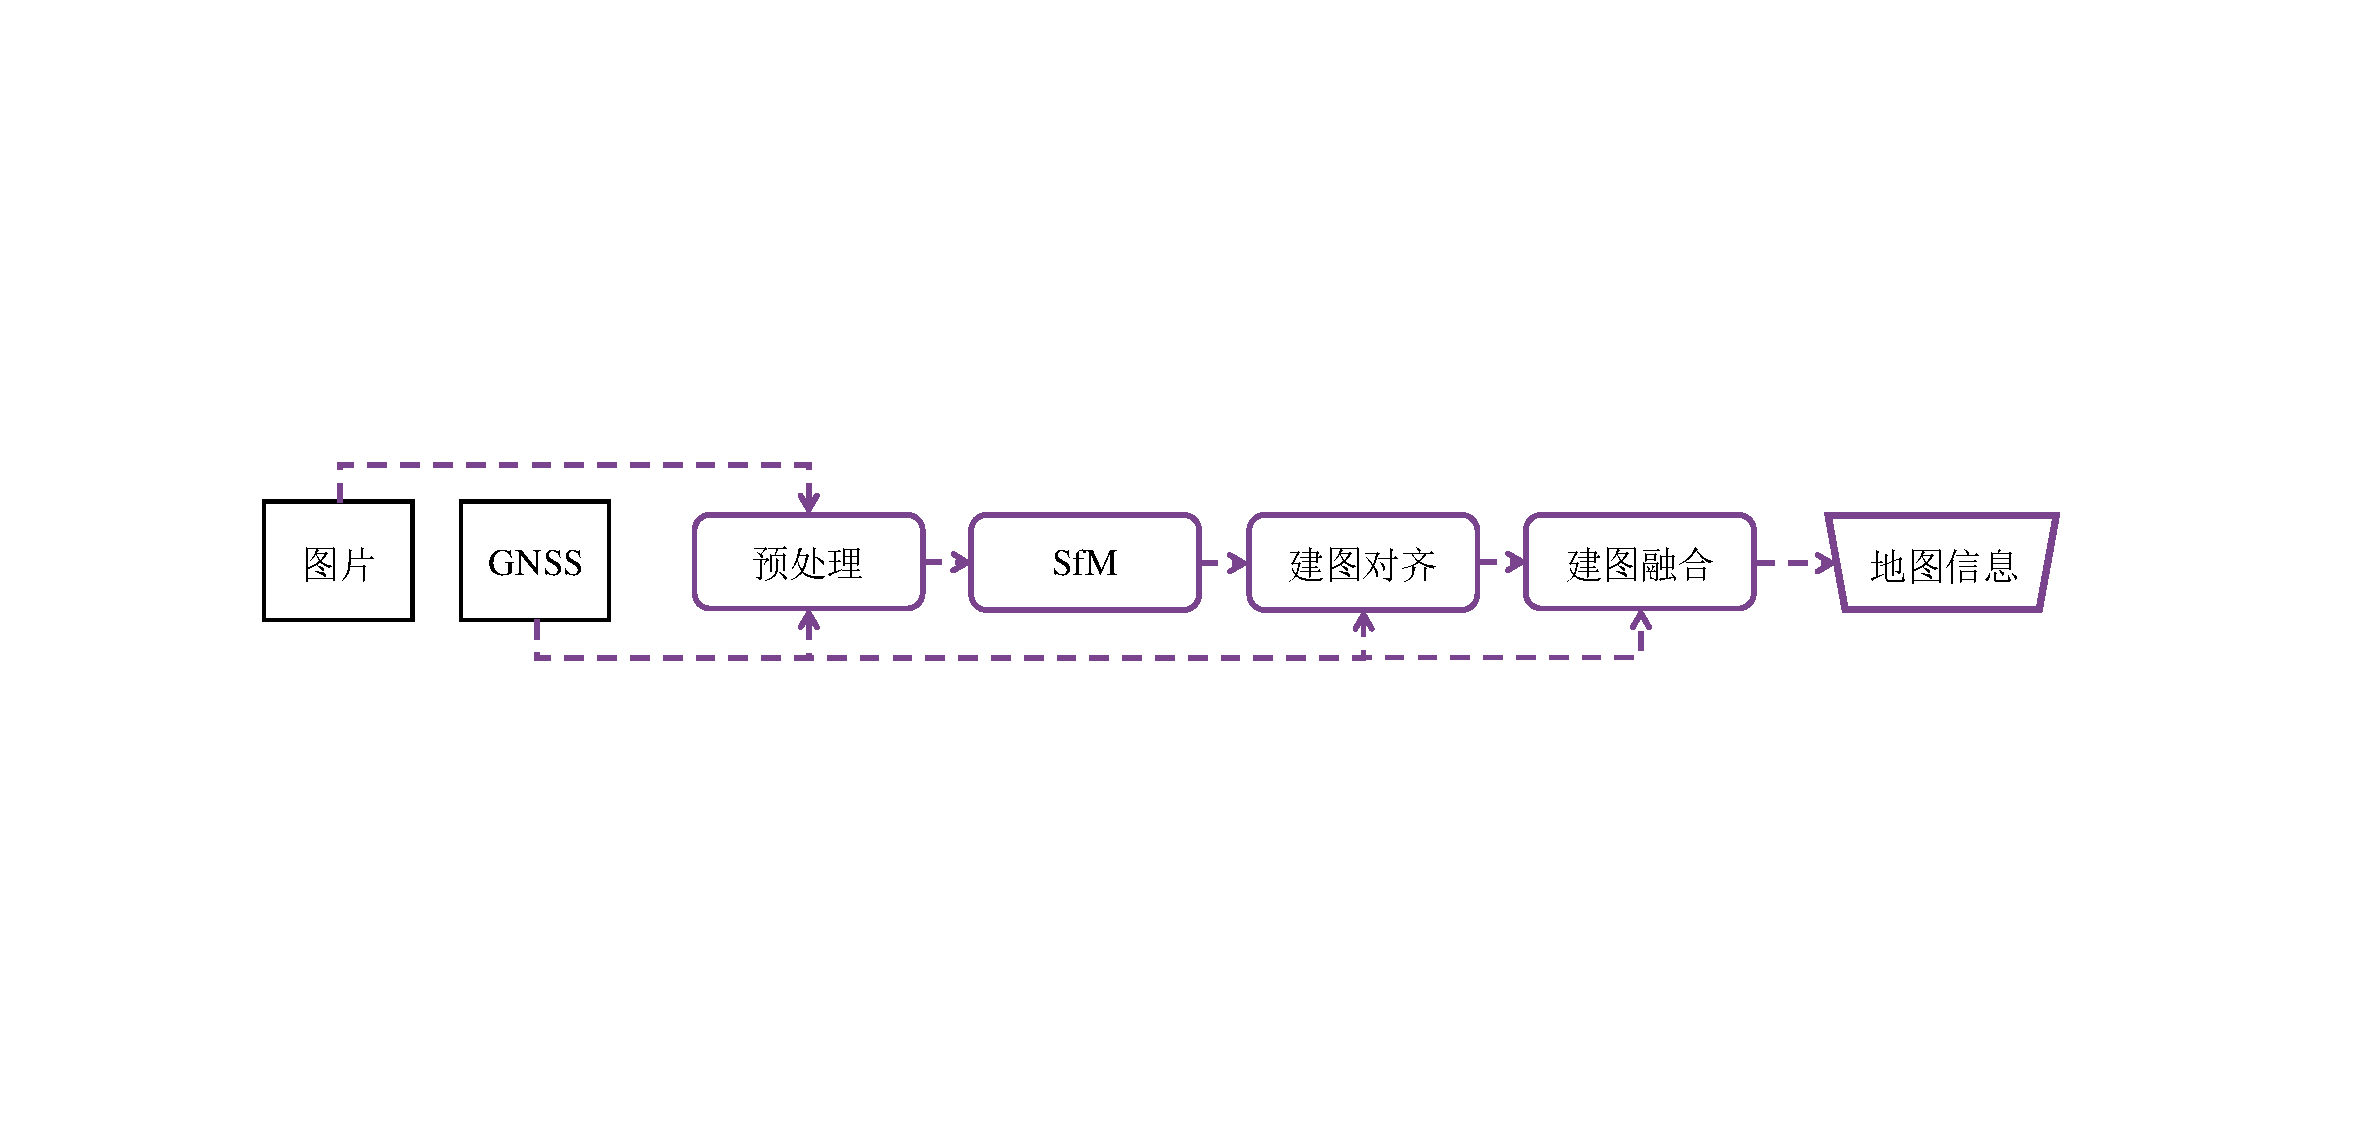
\includegraphics[width=1.0\linewidth]{mapping.pdf}
  \caption{离线建图模块整体流程}
  \label{fig:mapping}
\end{figure}

离线建图模块的整体流程如图\ref{fig:mapping}所示:首先通过图片和GNSS信息进行预处理,主要是筛选出候选关键帧以及进行语义分割(Semantic Segmentation)等操作;紧接着纯图像首先进行SfM以获得在视觉建图世界坐标系下的相机位姿和地图点云;然后使用GNSS信息和SfM结果进行建图对齐,即实现视觉建图世界坐标系和全局坐标系的对齐;此后进行建图融合,以非线性优化的方式同时优化视觉重投影误差和GNSS提供的位置误差;最后输出分层次的的地图。

值得注意的是,在建图阶段本文并没有使用到惯性信息,这主要由于惯性信息的使用必须同时满足“时间连续”和“时间间隔合理”两个条件才可以获得较好的效果,否则,不连续的时间会导致积分中断,过长的时间间隔会导致积分误差过大,而本文所假设的建图情况并不一定同时满足上述两个条件,故而只使用图片和GNSS信息。

\section{建图预处理}
预处理部分的主要目的是提高建图的效率并准备好建图所需数据,具体工作是根据图像和GNSS信息筛选出候选关键帧并根据建图需求对图片进行一系列处理,包括语义分割、特征提取和特征匹配。

\subsection{候选关键帧筛选}
在建图过程中,关键帧的选择对于建图效率和精度有着重要影响,关键帧的选择一般遵循以下的原则:(1)关键帧之间必须有足够的共视区域,这是为了保证有足够的特征点可以被匹配;(2)关键帧之间的距离不宜太小,这是为了降低重投影误差对地图点云精度的影响,如图\ref{fig:keyframe}所示,当地图点在相机2上偏移了同样一个角度$\delta \theta$时,对地图点的估计误差会因为帧间相对距离的不同而有差异,而当帧间位移较小的时候,误差明显加大。为了达成原则(1),本文使用连续的图像帧作为候选关键帧,保证了候选关键帧之间有足够的共视区域。为了达成原则(2),本文使用了GNSS提供的位置信息来过滤掉距离过近的候选关键帧,设定过滤阈值为1.5m,即如果两个候选关键帧之间的距离小于1.5m,则保留其中一个,否则保留两者。

\begin{figure}
  \centering
  \begin{tikzpicture}[x=0.75pt,y=0.75pt,yscale=-1,xscale=1]
  %uncomment if require: \path (0,300); %set diagram left start at 0, and has height of 300

  %Straight Lines [id:da9271411216933381] 
  \draw    (92,141) -- (134,15) ;
  \draw [shift={(92,141)}, rotate = 288.43] [color={rgb, 255:red, 0; green, 0; blue, 0 }  ][fill={rgb, 255:red, 0; green, 0; blue, 0 }  ][line width=0.75]      (0, 0) circle [x radius= 3.35, y radius= 3.35]   ;
  %Straight Lines [id:da29003793579323167] 
  \draw    (92,141) -- (156,141) ;
  \draw [shift={(159,141)}, rotate = 180] [fill={rgb, 255:red, 0; green, 0; blue, 0 }  ][line width=0.08]  [draw opacity=0] (10.72,-5.15) -- (0,0) -- (10.72,5.15) -- (7.12,0) -- cycle    ;
  %Straight Lines [id:da5112353172737918] 
  \draw    (125,14) -- (159,141) ;
  \draw [shift={(159,141)}, rotate = 75.01] [color={rgb, 255:red, 0; green, 0; blue, 0 }  ][fill={rgb, 255:red, 0; green, 0; blue, 0 }  ][line width=0.75]      (0, 0) circle [x radius= 3.35, y radius= 3.35]   ;
  %Shape: Circle [id:dp1662355167840721] 
  \draw  [fill={rgb, 255:red, 0; green, 0; blue, 0 }  ,fill opacity=1 ] (124,30) .. controls (124,27.24) and (126.24,25) .. (129,25) .. controls (131.76,25) and (134,27.24) .. (134,30) .. controls (134,32.76) and (131.76,35) .. (129,35) .. controls (126.24,35) and (124,32.76) .. (124,30) -- cycle ;
  %Straight Lines [id:da6367497127041384] 
  \draw  [dash pattern={on 4.5pt off 4.5pt}]  (98,31) -- (159,141) ;
  %Straight Lines [id:da03601324600093769] 
  \draw    (139,104) -- (148,99) ;
  %Straight Lines [id:da9735029157865975] 
  \draw    (279,141) -- (336,17) ;
  \draw [shift={(279,141)}, rotate = 294.69] [color={rgb, 255:red, 0; green, 0; blue, 0 }  ][fill={rgb, 255:red, 0; green, 0; blue, 0 }  ][line width=0.75]      (0, 0) circle [x radius= 3.35, y radius= 3.35]   ;
  %Straight Lines [id:da52354703700931] 
  \draw    (279,141) -- (428,141) ;
  \draw [shift={(431,141)}, rotate = 180] [fill={rgb, 255:red, 0; green, 0; blue, 0 }  ][line width=0.08]  [draw opacity=0] (10.72,-5.15) -- (0,0) -- (10.72,5.15) -- (7.12,0) -- cycle    ;
  %Straight Lines [id:da9759107264201796] 
  \draw    (312,14) -- (431,141) ;
  \draw [shift={(431,141)}, rotate = 46.86] [color={rgb, 255:red, 0; green, 0; blue, 0 }  ][fill={rgb, 255:red, 0; green, 0; blue, 0 }  ][line width=0.75]      (0, 0) circle [x radius= 3.35, y radius= 3.35]   ;
  %Shape: Circle [id:dp7881999863696054] 
  \draw  [fill={rgb, 255:red, 0; green, 0; blue, 0 }  ,fill opacity=1 ] (324,33) .. controls (324,30.24) and (326.24,28) .. (329,28) .. controls (331.76,28) and (334,30.24) .. (334,33) .. controls (334,35.76) and (331.76,38) .. (329,38) .. controls (326.24,38) and (324,35.76) .. (324,33) -- cycle ;
  %Straight Lines [id:da010281824834210473] 
  \draw  [dash pattern={on 4.5pt off 4.5pt}]  (299,46) -- (431,141) ;
  %Straight Lines [id:da5937501580461493] 
  \draw    (381,104) -- (390,97) ;
  %Straight Lines [id:da707089378321986] 
  \draw [color={rgb, 255:red, 155; green, 155; blue, 155 }  ,draw opacity=1 ] [dash pattern={on 4.5pt off 4.5pt}]  (70,141) -- (466,141) ;

  % Text Node
  \draw (70,148) node [anchor=north west][inner sep=0.75pt]   [align=left] {相机1};
  % Text Node
  \draw (148,148) node [anchor=north west][inner sep=0.75pt]   [align=left] {相机2};
  % Text Node
  \draw (136,18) node [anchor=north west][inner sep=0.75pt]   [align=left] {地图点P};
  % Text Node
  \draw (150,88.4) node [anchor=north west][inner sep=0.75pt]  [font=\footnotesize]  {$\delta \theta $};
  % Text Node
  \draw (86,13.4) node [anchor=north west][inner sep=0.75pt]  [font=\footnotesize]  {$\delta d$};
  % Text Node
  \draw (257,148) node [anchor=north west][inner sep=0.75pt]   [align=left] {相机1};
  % Text Node
  \draw (415,147) node [anchor=north west][inner sep=0.75pt]   [align=left] {相机2};
  % Text Node
  \draw (351,20) node [anchor=north west][inner sep=0.75pt]   [align=left] {地图点P};
  % Text Node
  \draw (393,84.4) node [anchor=north west][inner sep=0.75pt]  [font=\footnotesize]  {$\delta \theta $};
  % Text Node
  \draw (294,30.4) node [anchor=north west][inner sep=0.75pt]  [font=\footnotesize]  {$\delta d$};
  % Text Node
  \draw (123,122.4) node [anchor=north west][inner sep=0.75pt]    {$t$};
  % Text Node
  \draw (335,122.4) node [anchor=north west][inner sep=0.75pt]    {$t$};


  \end{tikzpicture}
  \caption{关键帧之间的距离会影响地图点精度}
  \label{fig:keyframe}
\end{figure}

\subsection{语义分割}

在候选关键帧筛选之后,接下来是对图片进行语义分割。语义分割可以利用图片中的高层语义分析,协助达成SfM的静态环境假设,即SfM所重建出来的地图点云应归属于静态物体。在实际的道路建图中,这一条件的达成并不容易,例如在城市环境下,建筑物是理想的建图元素,因为其位置相对固定,短时间内外观变化较小,但是汽车、行人等元素则不适合作为建图元素,因为其位置可能变化,并且处于移动状态会使得不同时刻的相机观测不满足静态假设。因此,本文使用语义分割算法对图片进行处理,将图片中动态物体剔除,保留静态部分以便建立更加稳定和精确的地图。

\begin{table}
  \centering
  \caption{语义分割类别分布与屏蔽情况}
  \begin{tabular}{cccccccccccc}
  \toprule
  类别 & road & ... & sky & person & rider & car & truck & bus & train & motorcycle & bicycle \\
  \midrule
  标签序号 & 0    &  ... & 10  & 11 & 12 & 13 & 14 & 15  & 16 & 17 & 18 \\
  屏蔽   &     &    &    & \checkmark &  \checkmark    &  \checkmark  &  \checkmark &  \checkmark  &   \checkmark   &  \checkmark  & \checkmark \\ 
  \bottomrule 
  \end{tabular}
  \label{tab:seg}
\end{table}

因为语义分割技术只是离线建图工作中的一小部分,所以本文选择了开箱即用的语义分割模型,并根据建图模块的实际需求进行了微调。本文所选择的语义分割模型是SegFormer\cite{xie2021segformer},SegFormer是一个基于Transformer的语义分割模型,凭借其紧凑但高效的网络结构,其在语义分割精度和速度上均取得了较好的效果。本文使用了SegFormer的B1型,即SegFormer-B1在cityscapes\cite{Cordts2016Cityscapes}数据集上的预训练权重作为初始,在该数据集的灰度图像上进行了微调。cityscapes数据集是一个城市道路环境下的语义分割数据集,包含了大量的城市道路图片和对应的标签,标签中包含了道路、建筑、树木等静态物体的信息,以及汽车、行人等动态物体。微调以$1024 \times 1024$的分辨率进行了160,000轮迭代,使得模型在灰度图上的表现接近了其在彩色图片上的表现,以便在建图过程中适应建图所使用的灰度图像输入。

\begin{figure}
  \centering
  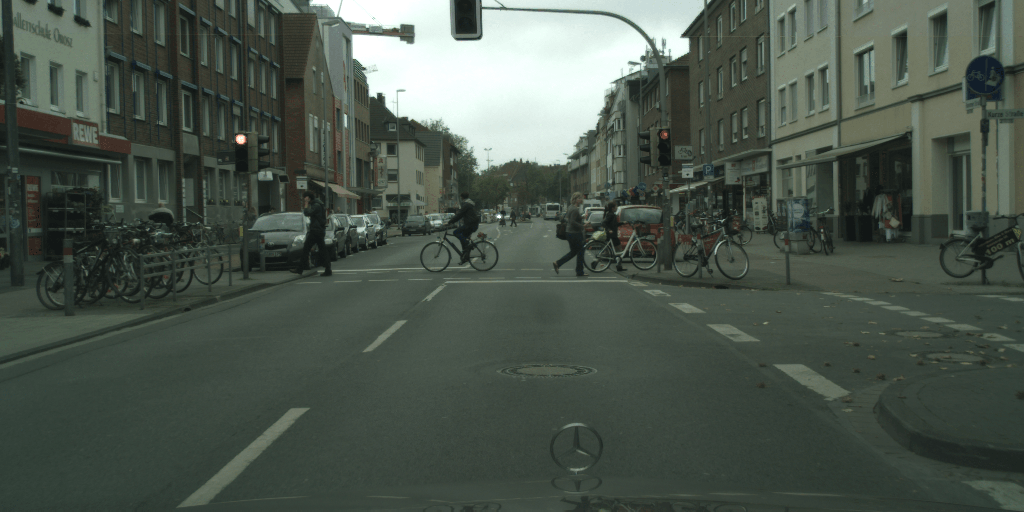
\includegraphics[width=0.47\linewidth]{seg.png}
  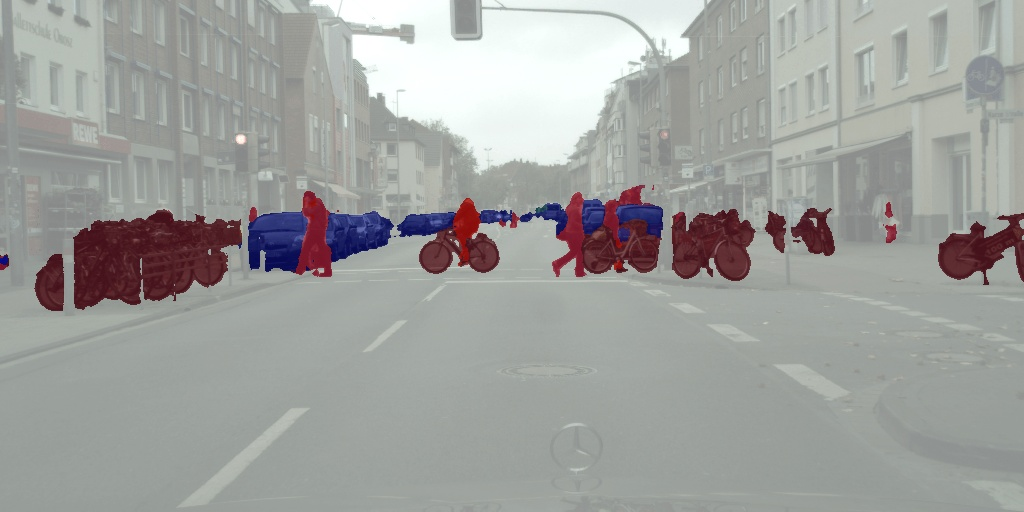
\includegraphics[width=0.47\linewidth]{seged.jpg}
  \caption{语义分割效果}
  \label{fig:seg}
\end{figure}

本文的语义分割模型在cityscapes数据集上训练,其输出的类别以及每一类别的标签序号如表~\ref{tab:seg}所示。在建图过程中,本文会将潜在的移动物体类别所包含的像素位置标记为屏蔽,后续的特征提取和匹配过程将不考虑这些像素位置,具体的屏蔽情况也汇报在表~\ref{tab:seg}中。语义分割的实际效果以及屏蔽内容以图~\ref{fig:seg}所示,左侧为原始图像,右侧为语义分割的结果示意图,其中被白色覆盖的区域为保留部分,被其他颜色覆盖的区域为屏蔽部分,可以看到被屏蔽的大部分区域均为行人、自行车等动态物体。

\section{SfM}

经过建图预处理的图像会进行SfM,构建初步的点云地图。SfM是一种摄影测量技术,用于从二维图像序列中估计三维结构\cite{schonberger2016structure}。SfM以地图关键帧序列$\mathcal{K} = \{K_i \mid i=1 \ldots N_{K} \}$和相机内参矩阵$\mathbf{K}$作为输入,输出地图关键帧序列的六自由度位姿$\mathcal{T} = \{\mathbf{T}^{k_i}_w \mid i=1 \ldots N_K \}$以及空间点集$\mathcal{P} = \{\mathbf{p}_{m}^{w} \in \mathbb{R}^3 \mid m=1 \ldots N_P\}$,统称为稀疏点云结构。需要注意的是,相机内参矩阵数量本应与地图关键帧数量对应,但是对于固定路线定位来说,建图所用图像均由同一相机拍摄,因此共用一个内参。

SfM通常以特征检测和匹配为第一步:对于每个地图关键帧$K_i$,SfM检测出一组局部特征$\mathcal{F}_i = \{(\mathbf{x}_j, \mathbf{f}_j) \mid j = 1, \ldots, N_{F_i}\}$,其中 $\mathbf{x}_j \in \mathbb{R}^2$表示特征点的位置,$\mathbf{f}_j \in \mathbb{R}^{d_l}$ 表示其 ${d_l}$ 维特征描述子。随后,进行图像匹配以识别捕捉到同一场景区域的关键帧,在这个过程中基于描述子的匹配方法被广泛采用。在本文中,由于建图预处理部分已经对地图关键帧的相对位置进行了筛选,因此相邻的关键帧已经具有了足够的共视区域,可以直接进行匹配,简化了匹配过程。

在相邻帧之外,为了通过闭环检测减轻漂移的问题,本文在建图时还引入了基于闭环检测的匹配方法。回环检测通过为每个关键帧提取一个$d_g$维的图像描述子$\mathbf{D}_i \in \mathbb{R}^{d_g}$,并计算所有地图关键帧之间图像描述子的相似度得分来实现,得分超过预设阈值$s$的前$m$对被选为回环闭合对。对于所有匹配上的地图关键帧对,SfM通过特征点描述子匹配特征点,并利用这些匹配点估计两个关键帧之间的相对位姿。

在完成特征检测和匹配之后,SfM进一步估计地图关键帧的位姿以及结构的空间坐标。通过选择第一个地图关键帧作为视觉建图世界坐标系的原点,所有关键帧的位姿$\mathcal{T}$都可以递归得通过相对位姿转换进行粗略估计。随后,SfM用三角化方法在视觉建图世界坐标系中估计稀疏点云结构$\mathcal{P}$的粗略空间坐标。位姿估计与三角化过程密切相关:位姿的不确定性会导致三角化点的可靠性下降,反之亦然。因此,为了获得精确的 $\mathcal{T}$ 和 $\mathcal{P}$,更精确的优化过程必不可少。

光束法平差(Bundle Adjustment, BA)是一种高效的位姿和点云结构优化方法,可通过最小化重投影误差来同时两种参数:
\begin{equation}
\label{eq:reproj_error}
E_i = \sum_{j}\rho(\Vert \hat{\mathbf{x}}_j - \pi(\mathbf{T}^{k_i}_w, \mathbf{p}_{m}^{w}) \Vert ^2_2),
\end{equation}
其中,$\mathbf{p}_{m}^{w}$是图像特征点$\hat{\mathbf{x}}_j$对应的空间点三维坐标,$\rho$是一种损失函数,用于降低异常值的权重。函数 $\pi(\cdot)$ 将空间点投影到图像空间,定义如下:
\begin{equation}
\label{eq:proj_func}
\pi(\mathbf{T}^{k_i}_w, \mathbf{p}_{m}^{w}) = [\mathbf{K}\cdot(\mathbf{R}_w^{k_i}\cdot\mathbf{p}_{m}^{w}+\mathbf{t}_w^{k_i})/d_j]_{0:2},
\end{equation}
其中,$d_j$ 是 $\mathbf{p}_{m}^{w}$ 在相机坐标系中的深度,$[\cdot]_{0:2}$ 表示选择向量的前两个元素。需要注意的是,$E_i$ 表示单张图像的重投影误差,因此整个BA是对输入图像序列中的所有重投影误差进行累积优化的结果。BA的进行需要使用非线性优化方法,例如高斯-牛顿法或者Levenberg-Marquardt法,而使用这两种方法需要求解误差函数\ref{eq:reproj_error}关于待求解参数$\mathbf{T}^{k_i}_w$和$\mathbf{p}_{m}^{w}$的雅可比矩阵,非线性优化过程及雅可比矩阵的推导参考附录~\ref{appendix:quat}。


\section{建图对齐}

SfM可以为离线建图阶段的图像提供精化的位姿和稀疏点云地图,但这些位姿和结构并不是在全局坐标系下的,并且缺乏真实世界的物理尺度,因此不适用于实际的定位任务。为了解决这一问题,本文利用图像的对应GNSS观测数据,将SfM的输出与真实世界的物理尺度对齐。标准GNSS报文仅提供地理坐标系中的纬度、经度和海拔信息,地理坐标系是一种墨卡托坐标系,而地图关键帧位姿和点云结构都是在笛卡尔坐标系中。因此,需要首先将原始GNSS报文信息从地理坐标系统转换为笛卡尔ENU坐标系中的位置序列
$\mathcal{L} = \{\mathbf{l}_{k_i}^g \in \mathbb{R}^3 \mid i=1 \ldots N_K \}$。
这一过程遵循Subirana等人 \cite{subirana2011transformations} 提出的转换方法,并设置
$\mathbf{l}_{k_1}^g = \mathbf{0}$ 以确保数值稳定性。

由于建图对齐过程不仅需要解决视觉建图世界坐标系与全局坐标系之间的变换问题,还需要处理两者之间的尺度差异,本课题采用三维相似变换(Similarity Transformation in 3D, Sim3)~\cite{horn1987closed}。Sim3包括一个比例因子 $s$、一个旋转矩阵 $\mathbf{R}_w^g$ 和一个平移向量 $\mathbf{t}_w^g$。如果第 $i$ 个地图关键帧在视觉建图世界坐标系中的位置为 $\mathbf{t}_{k_i}^{w} = -{\mathbf{R}_w^{c_i}}^T \cdot \mathbf{t}_w^{k_i}$,对应的 GNSS 观测值为 $\mathbf{l}_{k_i}^g$,则Sim3变换可以将它们对齐,具体如下:
\begin{equation}
    \mathbf{l}_{k_i}^g = s \cdot \mathbf{R}_w^g \cdot \mathbf{t}_{k_i}^{w} + \mathbf{t}_w^g.
\end{equation}
Sim3 参数的最小二乘解可以通过求解以下优化问题获得:
\begin{equation}
  s^*, {\mathbf{R}_w^g}^*, {\mathbf{t}_w^g}^* = \underset{s,\mathbf{R}_w^g,\mathbf{t}_w^g}{\text{arg min}} \sum_i^{N_I} \Vert \mathbf{l}_{k_i}^g - s \cdot \mathbf{R}_w^g \cdot \mathbf{t}_{k_i}^{w} - \mathbf{t}_w^g \Vert_2^2.
\end{equation}

利用 Sim3 参数,可以方便地将地图关键帧位姿 $\mathcal{T}$ 和稀疏点云结构 $\mathcal{P}$ 转换到具有真实物理尺度的全局坐标系中:
\begin{equation}
\begin{cases}
    \mathbf{R}^{k_i}_g = {\mathbf{R}^{k_i}_{w}} \cdot {\mathbf{R}_w^g}^{-1}, \\
    \mathbf{t}^{k_i}_g = s \cdot \mathbf{t}_w^{c_i} - {\mathbf{R}^{k_i}_{w}} \cdot {\mathbf{R}^{g}_{w}}^{-1} \mathbf{t}_w^g, \\
    \mathbf{p}_m^g = s \cdot \mathbf{R}_w^g \cdot \mathbf{p}_{m}^{w} + \mathbf{t}_w^g,
\end{cases}.
\end{equation}

\section{建图融合}

尽管已经获得了较为精确的地团关键帧位姿和稀疏点云结构,并成功将它们转换到全局坐标系中,但在求解Sim3参数的最小二乘解时仍可能引入误差。为了获得更精确的位姿和点云结构,还需要将当前的全局坐标系参数与GNSS观测进行融合优化。该融合过程需要确保地图关键帧位姿和点云结构同时满足GNSS和视觉的观测,因此需要在视觉BA的基础上融合进GNSS的观测约束,将全局坐标系中的重投影误差重新表示为:
\begin{equation}
\label{eq:new_reproj}
    E_i = \sum_{j}\rho\left(\Vert \mathbf{x}_j - \pi(\mathbf{T}^{k_i}_g, \mathbf{p}_{m}^{g}) \Vert ^2_2\right) 
    + \alpha \cdot \rho\left(\Vert -\mathbf{R}_g^{k_i^T}\cdot\mathbf{t}_g^{k_i} - \mathbf{l}_{k_i}^g \Vert_2^2\right),
\end{equation}
其中,$\alpha$ 是一个权重系数,用于平衡视觉重投影误差与位置偏差。然后通过BA过程对式 \eqref{eq:new_reproj} 中的误差进行最小化。

至此,已经介绍了地图关键帧位姿和稀疏点云结构的优化,这些空间信息有效地描述了环境结构。然而,为了在定位过程中充分利用这些信息,还需要视觉地图关键帧和稀疏点云的描述符,用于地图与实时捕获图像之间的匹配。在离线建图过程中,直接使用 $\{\mathcal{F}_i \mid i = 1, \ldots, N_K\}$ 作为地图点的描述符,$\{\mathbf{D}_i \mid i = 1, \ldots, N_K\}$ 作为关键帧描述符。离线建图模块的最终输出可以分为两个层级:粗粒度层级和细粒度层级。粗粒度层级输出包括关键帧位姿和描述符,用于建立图像匹配关系;而细粒度层级输出包括点描述符和点结构,用于实现点的匹配。

\section{本章总结}
本章主要介绍了固定路线定位系统的整体架构和离线建图模块的设计。整体架构中建图与定位以异构的形式存在,即建图以SfM技术为基础,而定位以SLAM技术为基础,这种异构设计能够充分发挥SfM的精度优势和SLAM的速度优势。离线建图模块以视觉和GNSS融合的SfM为基础,同时根据建图需求引入了基于深度学习的语义分割、回环检测以及特征点提取技术,将更多的人类经验加入到离线建图中。离线建图模块的另一个特点是在传统SfM的基础上引入了GNSS观测作为约束和融合信息,这能够显著提升建图的精度。

% !TeX root = ../thuthesis-example.tex

\chapter{视觉惯性里程计}

\section{整体设计}
视觉惯性里程计是视觉惯性定位中的关键组成部分,其主要工作是为定位提供较为精确的帧间运动关系约束,这对于最终的定位精度有着不可忽视的作用。视觉惯性里程计常用于无人机、自动驾驶车辆和机器人等领域,传统的视觉惯性里程计一般考虑机体做任意运动,因此仅构建了惯性和视觉观测之间的约束关系。而然,在固定路线的定位中,机体的运动往往自身同样具有一定的伪观测约束:本文考虑的汽车和轮式机器人,其运动往往在平面上进行,因此其速度一般可以分解为沿着车辆前进方向的速度和沿着车身横向的速度。如图~\ref{fig:vehicle}所示,实线代表IMU体坐标系$(\cdot)^{b_{j}}$,虚线代表车身坐标系$(\cdot)^{v_{j}}$,车身坐标系的$y$轴沿着车辆前进方向,$x$轴沿着车辆横向方向,$z$轴垂直于地面向上。IMU体坐标系即IMU的测量坐标系,其一般状态下与车身坐标系会存在一定的旋转关系,并不一定如图所示的共向。

\begin{figure}
  \centering
  \tikzset{every picture/.style={line width=0.75pt}} %set default line width to 0.75pt        
  \begin{tikzpicture}[x=0.75pt,y=0.75pt,yscale=-1,xscale=1]
  %uncomment if require: \path (0,300); %set diagram left start at 0, and has height of 300

  %Image [id:dp3701434269039574] 
  \draw (145,144.74) node  {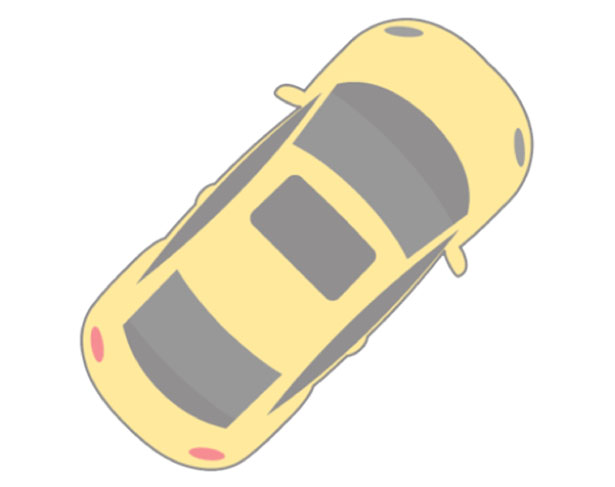
\includegraphics[width=99pt,height=74.61pt]{vehicle.png}};
  %Straight Lines [id:da20058009351259742] 
  \draw [color={rgb, 255:red, 74; green, 144; blue, 226 }  ,draw opacity=1 ][line width=1.5]  [dash pattern={on 5.63pt off 4.5pt}]  (146,146) -- (217.39,111.73) ;
  \draw [shift={(221,110)}, rotate = 154.36] [fill={rgb, 255:red, 74; green, 144; blue, 226 }  ,fill opacity=1 ][line width=0.08]  [draw opacity=0] (10.92,-2.73) -- (0,0) -- (10.92,2.73) -- cycle    ;
  %Straight Lines [id:da5603181046378807] 
  \draw [color={rgb, 255:red, 208; green, 2; blue, 27 }  ,draw opacity=1 ][line width=1.5]  [dash pattern={on 5.63pt off 4.5pt}]  (146,146) -- (195.98,189.38) ;
  \draw [shift={(199,192)}, rotate = 220.96] [fill={rgb, 255:red, 208; green, 2; blue, 27 }  ,fill opacity=1 ][line width=0.08]  [draw opacity=0] (10.92,-2.73) -- (0,0) -- (10.92,2.73) -- cycle    ;
  %Straight Lines [id:da43883225903692824] 
  \draw [color={rgb, 255:red, 65; green, 117; blue, 5 }  ,draw opacity=1 ][line width=1.5]  [dash pattern={on 5.63pt off 4.5pt}]  (146,146) -- (202.29,84.94) ;
  \draw [shift={(205,82)}, rotate = 132.67] [fill={rgb, 255:red, 65; green, 117; blue, 5 }  ,fill opacity=1 ][line width=0.08]  [draw opacity=0] (10.92,-2.73) -- (0,0) -- (10.92,2.73) -- cycle    ;
  %Straight Lines [id:da4769565351313416] 
  \draw [color={rgb, 255:red, 74; green, 144; blue, 226 }  ,draw opacity=1 ][line width=1.5]    (146.28,144.45) -- (221.23,118.89) ;
  \draw [shift={(225.02,117.6)}, rotate = 161.17] [fill={rgb, 255:red, 74; green, 144; blue, 226 }  ,fill opacity=1 ][line width=0.08]  [draw opacity=0] (10.92,-2.73) -- (0,0) -- (10.92,2.73) -- cycle    ;
  %Straight Lines [id:da3562334885093257] 
  \draw [color={rgb, 255:red, 208; green, 2; blue, 27 }  ,draw opacity=1 ][line width=1.5]    (146.28,144.45) -- (190.76,193.45) ;
  \draw [shift={(193.45,196.41)}, rotate = 227.77] [fill={rgb, 255:red, 208; green, 2; blue, 27 }  ,fill opacity=1 ][line width=0.08]  [draw opacity=0] (10.92,-2.73) -- (0,0) -- (10.92,2.73) -- cycle    ;
  %Straight Lines [id:da672459548829603] 
  \draw [color={rgb, 255:red, 65; green, 117; blue, 5 }  ,draw opacity=1 ][line width=1.5]    (146.28,144.45) -- (209.41,90.5) ;
  \draw [shift={(212.45,87.9)}, rotate = 139.48] [fill={rgb, 255:red, 65; green, 117; blue, 5 }  ,fill opacity=1 ][line width=0.08]  [draw opacity=0] (10.92,-2.73) -- (0,0) -- (10.92,2.73) -- cycle    ;
  %Straight Lines [id:da7351111533191295] 
  \draw [color={rgb, 255:red, 65; green, 117; blue, 5 }  ,draw opacity=1 ][line width=1.5]  [dash pattern={on 5.63pt off 4.5pt}]  (286,159) -- (342.29,97.94) ;
  \draw [shift={(345,95)}, rotate = 132.67] [fill={rgb, 255:red, 65; green, 117; blue, 5 }  ,fill opacity=1 ][line width=0.08]  [draw opacity=0] (10.92,-2.73) -- (0,0) -- (10.92,2.73) -- cycle    ;
  %Straight Lines [id:da5481629305422135] 
  \draw [color={rgb, 255:red, 65; green, 117; blue, 5 }  ,draw opacity=1 ][line width=1.5]  [dash pattern={on 1.69pt off 2.76pt}]  (447,152) -- (503.29,90.94) ;
  \draw [shift={(506,88)}, rotate = 132.67] [fill={rgb, 255:red, 65; green, 117; blue, 5 }  ,fill opacity=1 ][line width=0.08]  [draw opacity=0] (10.92,-2.73) -- (0,0) -- (10.92,2.73) -- cycle    ;
  %Straight Lines [id:da7036682415956479] 
  \draw [color={rgb, 255:red, 208; green, 2; blue, 27 }  ,draw opacity=1 ][line width=1.5]  [dash pattern={on 1.69pt off 2.76pt}]  (447,152) -- (468.05,171.3) ;
  \draw [shift={(471,174)}, rotate = 222.51] [fill={rgb, 255:red, 208; green, 2; blue, 27 }  ,fill opacity=1 ][line width=0.08]  [draw opacity=0] (10.92,-2.73) -- (0,0) -- (10.92,2.73) -- cycle    ;
  %Straight Lines [id:da1265383231355004] 
  \draw [color={rgb, 255:red, 245; green, 166; blue, 35 }  ,draw opacity=1 ][line width=1.5]  [dash pattern={on 5.63pt off 4.5pt}]  (447,152) -- (522.51,109.95) ;
  \draw [shift={(526,108)}, rotate = 150.88] [fill={rgb, 255:red, 245; green, 166; blue, 35 }  ,fill opacity=1 ][line width=0.08]  [draw opacity=0] (10.92,-2.73) -- (0,0) -- (10.92,2.73) -- cycle    ;

  % Text Node
  \draw (195,194.4) node [anchor=north west][inner sep=0.75pt]  [font=\footnotesize,color={rgb, 255:red, 208; green, 2; blue, 27 }  ,opacity=1 ]  {$x$};
  % Text Node
  \draw (210,69.4) node [anchor=north west][inner sep=0.75pt]  [font=\footnotesize,color={rgb, 255:red, 65; green, 117; blue, 5 }  ,opacity=1 ]  {$y$};
  % Text Node
  \draw (229,106.4) node [anchor=north west][inner sep=0.75pt]  [font=\footnotesize]  {$\textcolor[rgb]{0.29,0.56,0.89}{z}$};
  % Text Node
  \draw (160,176.4) node [anchor=north west][inner sep=0.75pt]  [font=\large]  {$b_{j}$};
  % Text Node
  \draw (186,155.4) node [anchor=north west][inner sep=0.75pt]  [font=\large]  {$v_{j}$};
  % Text Node
  \draw (249,180) node [anchor=north west][inner sep=0.75pt]   [align=left] {直线行驶速度方向};
  % Text Node
  \draw (418,181) node [anchor=north west][inner sep=0.75pt]   [align=left] {转弯速度方向(黄色)};


  \end{tikzpicture}
  \caption{车身坐标系和IMU体坐标系分解示意}
  \label{fig:vehicle}
\end{figure}

在当前的坐标系下,假设车辆或机器人行驶在平面(不考虑上下坡导致的$z$轴速度),其状态可能存在3种情况:
\begin{enumerate}
  \item 车辆静止,此状态下车身坐标系的$y$与$x$轴均无速度;
  \item 直线行驶,此状态下车身坐标系的$y$轴有速度,$x$轴无速度;
  \item 车辆转弯,此状态下车身坐标系的$y$与$x$轴均有速度。
\end{enumerate}

据此分析,可以在车辆或机器人静止和直线行驶时,可以为车身增加两项伪观测,而这两项伪观测可以作为约束条件提升视觉惯性里程计的精度。但是,在仅依靠IMU信息和视觉信息的情况下,如何区分车辆的运动状态仍是一个有待解决的问题。此外,这两项约束如何添加到原有的视觉惯性里程计的优化中,也需要进一步的研究。未解决上述问题,本文在本章着重介绍如图~\ref{fig:vio_pipeline}所示的视觉惯性里程计。该视觉惯性里程计在一般设计的基础上加入了车身状态判别、惯性-车体粗对齐等过程,并在窗口优化中加入了惯性-车体因子,以上改动以绿色标注。

\begin{figure}
  \centering
  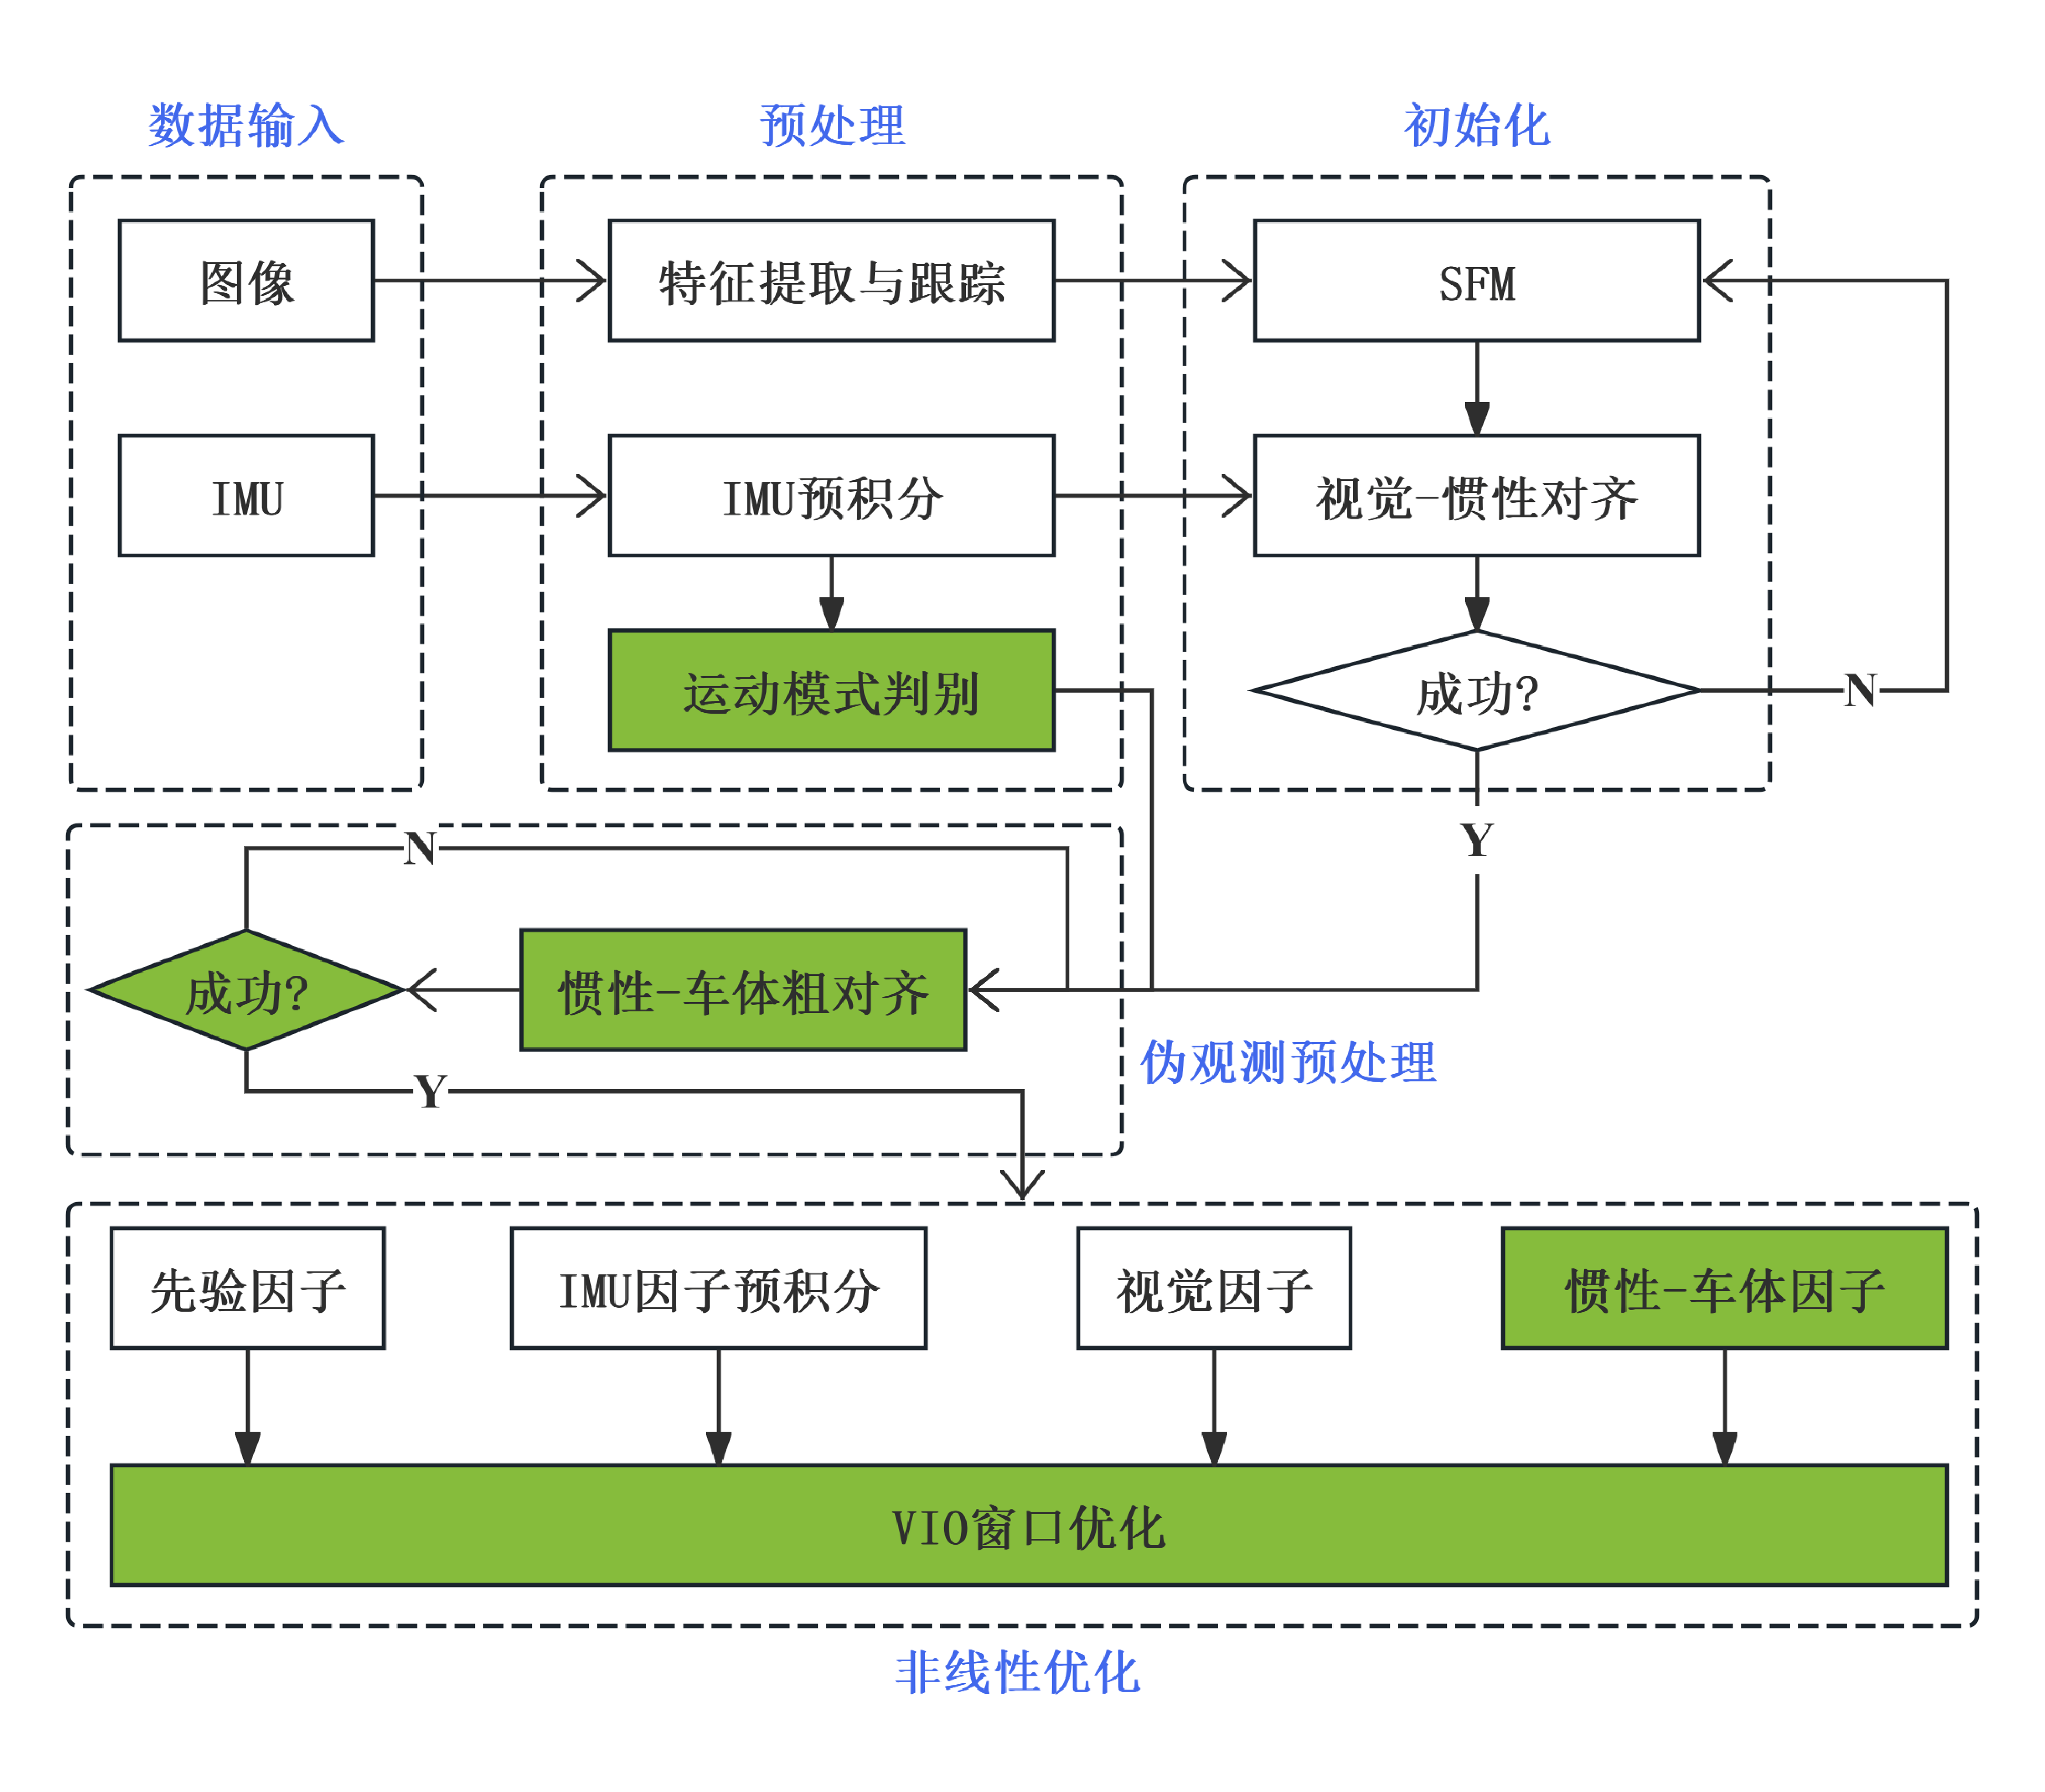
\includegraphics[width=0.9\linewidth]{VIO_pipeline.pdf}
  \caption{视觉惯性里程计框架}
  \label{fig:vio_pipeline}
\end{figure}

\section{车身状态判别}

根据对车身状态的分析,只有在车辆和机器人停止或直线行驶时,才能添加额外的约束。因此,需要在视觉惯性里程计中添加车身状态判别模块,以区分车辆的运动状态。以往的工作中,Hu等\cite{hu2020memsimu}使用传统的统计方法来判别车辆的直行、变道和转弯等状态;Brossard等\cite{brossard2020ai}使用卷积神经网络(Convolutional Neural Network, CNN)来生成车身3个轴向的测量噪声,以此来间接判别车辆状态;Huang等\cite{huang2022vehicle}则使用时间卷积神经网络(Temporal Convolutional Neural Network, TCN)根据IMU观测值来接判别车辆的运动状态。然而,基于统计的判别方法需要事先采集IMU静止状态下的数据进行统计分析,不够灵活;基于CNN和TCN的方法针对每一条IMU数据进行判别,这在应用于高频率IMU(例如2000Hz及以上)时会造成极大的时延。针对以上问题,本文希望使用一种更加灵活,并且有望实时进行的方法来进行车身状态判别。

近年来,因为深度学习技术在泛化性能上展现出的优势,本文希望使用基于深度学习的方法来进行车身状态判别。在输入信息的选择上,为了使得深度神经网络能够与IMU的处理频率相匹配,就必须放弃以往逐条处理IMU数据的模式,转而寻找一种批量处理IMU数据的模式。在传统的视觉惯性里程计中,IMU数据的处理采用预积分的形式,简单来说,这是一种将IMU数据的采集频率与图像数据的采集频率相匹配的处理方式。在这种形势下,两张相邻时间图像之间的IMU数据会被整合为一个预积分因子,这样就可以将IMU数据的处理频率降低到与图像数据相同的频率,这个频率一般在10Hz到30Hz。在这个频率下,基于深度神经网络的方式是有望实时进行的,因此预积分因子内包含的IMU数据序列是一个理想的网络输入。

但是,如果选择预积分因子内的IMU数据序列作为网络输入,那么就会面临一个问题:因为IMU频率和相近频率不一定是整除关系,所以两帧图像之间的IMU序列并不等长。这就导致了擅长处理规整数据的CNN或者TCN并不适合处理预积分因子内的IMU数据序列。近年来,基于Transformer结构的神经网络在自然语言处理领域展现出了优异的性能,其注意力机制使得其能够处理任意长度的序列数据,所以也十分适合处理所有序列化的数据。基于此优势考虑,本文选择以Transformer结构为基础,设计一个用于车身状态判别的深度神经网络。

\subsection{网络预测状态}
对于网络的预测状态,本文选择对车身的$y$轴(车身前向)速度和$x$轴(车身横向)速度状态进行判别。用向量
\begin{equation}
  \symbf{z} = 
    \begin{bmatrix}
      z^{\rm FOR}\\
      z^{\rm LAT} 
    \end{bmatrix} \in \{0, 1\}^{2}
\end{equation}
来表示车身静止假设和直线行驶假设是否成立。其中$z^{\rm FOR}$指示车身静止假设是否成立,其分布为
\begin{equation}
  z^{\rm FOR} =
  \begin{cases}
    0, & \text{车辆静止假设不成立} \\
    1, & \text{车辆静止假设成立}
  \end{cases}.
\end{equation}
$z^{\rm FOR}$表示车身横向速度为0假设是否成立,其分布为
\begin{equation}
  z^{\rm LAT} =
  \begin{cases}
    0, & \text{车辆横向速度为0假设不成立} \\
    1, & \text{车辆横向速度为0假设成立}
  \end{cases}.
\end{equation}

\subsection{网络输入选择}
对于网络输入,本文使用一个预积分因子内的IMU数据序列作为网络输入。单条IMU采样数据包括加速度计读数$\hat{\symbf{a}}^b \in \mathbb{R}^3$和陀螺仪读数$\hat{\symbf{\omega}}^b \in \mathbb{R}^3$,两个读数的可以分解为:
\begin{equation}
\begin{aligned}
  &\hat{\symbf{a}}^b = \symbf{a}^b + \symbf{R}^{b}_{g}\cdot \symbf{g} + \symbf{b}_{a} + \symbf{n}_{a} \\
  &\hat{\symbf{\omega}}^b = \symbf{\omega}^b + \symbf{b}_{\omega} + \symbf{n}_{\omega} 
\end{aligned}
\end{equation}
其中$\symbf{a}^b, \symbf{\omega}^b$分别表示IMU此时真正的加速度和角速度,$\symbf{b}_{\omega}, \symbf{b}_{a}$分别表示陀螺仪和加速度计的零偏,$\symbf{n}_{\omega}, \symbf{n}_{a}$分别表示陀螺仪和加速度计的噪声,$\symbf{R}^{b}_{g}$表示此时全局坐标系到IMU体坐标系的旋转矩阵,$\symbf{g}$表示地球重力加速度。单条读数可以反映某一时刻的IMU运动情况,因此如果结合采样时间对IMU序列进行积分,就可以获得一段时间内的IMU运动情况,即旋转和位移。因此,使用IMU序列数据,理论上足以预测车身状态。实践中,本文将单条加速度计和单条陀螺仪读数拼接为一个6维向量,作为一条完整的IMU采样数据。在此之后,将预积分因子内的多条IMU采样数据拼接为一个矩阵$\symbf{X}\in \mathbb{R}^{n \times 6}$用以表示IMU数据序列,其中$\mathbb{R}^{n \times 6}$表示$\symbf{X}$由$n$条IMU读数组成。

\subsection{网络结构设计}
\begin{table}
  \centering
  \caption{车身判别网络设计参数}
  \begin{tabular}{ccccccc}
  \toprule
  层 & 层类型                 & 输入维度 & 特征维度 & 前馈层维度 & 头数 & 输出维度 \\
  \midrule
  1 & 全连接层                & 6    & 128  & N/A   & N/A & 128 \\
  2 & Transformer Encoder & 128  & 128  & 1024  & 8 & 128  \\
  3 & Transformer Encoder & 128  & 128  & 1024  & 8 & 128  \\
  4 & Transformer Decoder & 128  & 128  & 1024  & 8 & 128  \\
  5 & Transformer Decoder & 128  & 128  & 1024  & 8 & 128  \\
  6 & 全连接层                & 128  & 2    & N/A   & N/A & 2 \\
  \bottomrule
  \end{tabular}
  \label{tab:network}
\end{table}

对于网络结构,本文希望其能够输入一个可变形状矩阵$\symbf{X}$,稳定输出向量$\symbf{z}$。因此,本文使用了经典的Encoder-Decoder架构Transformer\cite{vaswani2017attention}:其网络的基本参数如表~\ref{tab:network}所示。除了表中所示的神经网络层以外,本文网络中还有一个可训练参数$\symbf{q} \in \mathbb{R}^{128}$用于和两层Transformer Decoder进行交互已获得带有车身状态特征的向量$\symbf{q}' \in \mathbb{R}^{128}$,$\symbf{q}'$此后经全连接层获得预测向量$\symbf{y} \in \mathbb{R}^2$,$\symbf{y}$经过Sigmoid函数后得到预测的车身状态概率$\symbf{y} \in (0, 1)^2$。

\subsection{网络训练}

对于网络训练,需要明确的问题主要包括数据清洗、预测真值生成、损失函数设计和训练策略。
在数据清洗方面,由于IMU采样数据包括加速度和角速度,这两类数据的数值分布有较大差异:角速度以$rad/s$为单位,一般是一个较小的数字,加速度以$m/s^2$为单位,其取值范围一般较大。因此如果使用原始数据作为网络输入,往往会造成网络训练的不稳定,因此本文使用归一化策略,将所有的IMU采样数据元素调整为值域在$(-1, 1)$之间:首先根据训练数据的分布特征计算IMU采样数据的均值$\symbf{\mu}\in \mathbb{R}^6$和逐元素标准差$\symbf{\sigma}\in \mathbb{R}^6$,然后对每一条IMU数据根据
\begin{equation}
  \symbf{x}' = \frac{\symbf{x} - \symbf{\mu}}{\symbf{\sigma}}
\end{equation}
进行转换。$\symbf{x}$是一条包涵加速度和角速度的IMU数据,除法是逐元素除法,可以在相同形状的的数据上进行操作。

\renewcommand{\algorithmicrequire}{\textbf{输入:}\unskip}
\renewcommand{\algorithmicensure}{\textbf{输出:}\unskip}
\begin{algorithm}
  \caption{Generate training data and ground truth}
  \label{alg1}
  \small
  \begin{algorithmic}[1]
    \REQUIRE IMU时间戳序列$ts$, IMU采样数据序列$xs$, 车辆运动状态时间戳序列$vs$, 车辆位置状态序列$ps$, 车辆旋转状态序列$Rs$
    \ENSURE IMU数据序列列表$Xs$, 真值列表$zs$

    \STATE $vs$.insert(0, 0.0); $Xs \leftarrow []$; $Zs \leftarrow []$; $i \leftarrow 1$

    \WHILE{$i < $ len($vs$)}
      \STATE $j \leftarrow i-1$; $X \leftarrow []$; $z \leftarrow []$
      \WHILE{$ts[0] <= vs[j]$}
        \STATE $ts$.pop(0), $xs$.pop(0)
      \ENDWHILE
      \WHILE{$ts[0] <= vs[i]$}
        \STATE $X$.append($xs$.pop(0))
      \ENDWHILE
      \STATE $Xs$.append($X$)
      \IF{$ps[i] - ps[j] < {\epsilon}_p$}
        \STATE $z$.append(1)
      \ELSE
        \STATE $z$.append(0)
      \ENDIF
      \STATE convert rotation matrix $Rs[j]^T \cdot Rs[i]$ to roatation vector $v$
      \IF{norm($v$)$<{\epsilon}_r$}
        \STATE $z$.append(1)
      \ELSE
        \STATE $z$.append(0)
      \ENDIF
      \STATE $zs$.append($z$)
    \ENDWHILE
  \end{algorithmic}
\end{algorithm}

在预测真值生成方面,本文需要使用到车辆的真实运动状态。具体来说,首先根据车辆的真实运动状态的更新频率切分IMU序列,然后根据车身运动状态自动生成真值$\symbf{z}$。根据对预设状态的分类,首先根据相对位置信息判断车辆是否静止,然后根据相对旋转判断车辆是否直线行驶,具体如算法~\ref{alg1}所示,其中第16行即罗德里格斯旋转公式(Rodrigues' rotation formula)\cite{dai2015euler}将旋转矩阵转换为旋转向量。

\begin{figure}
  \centering
  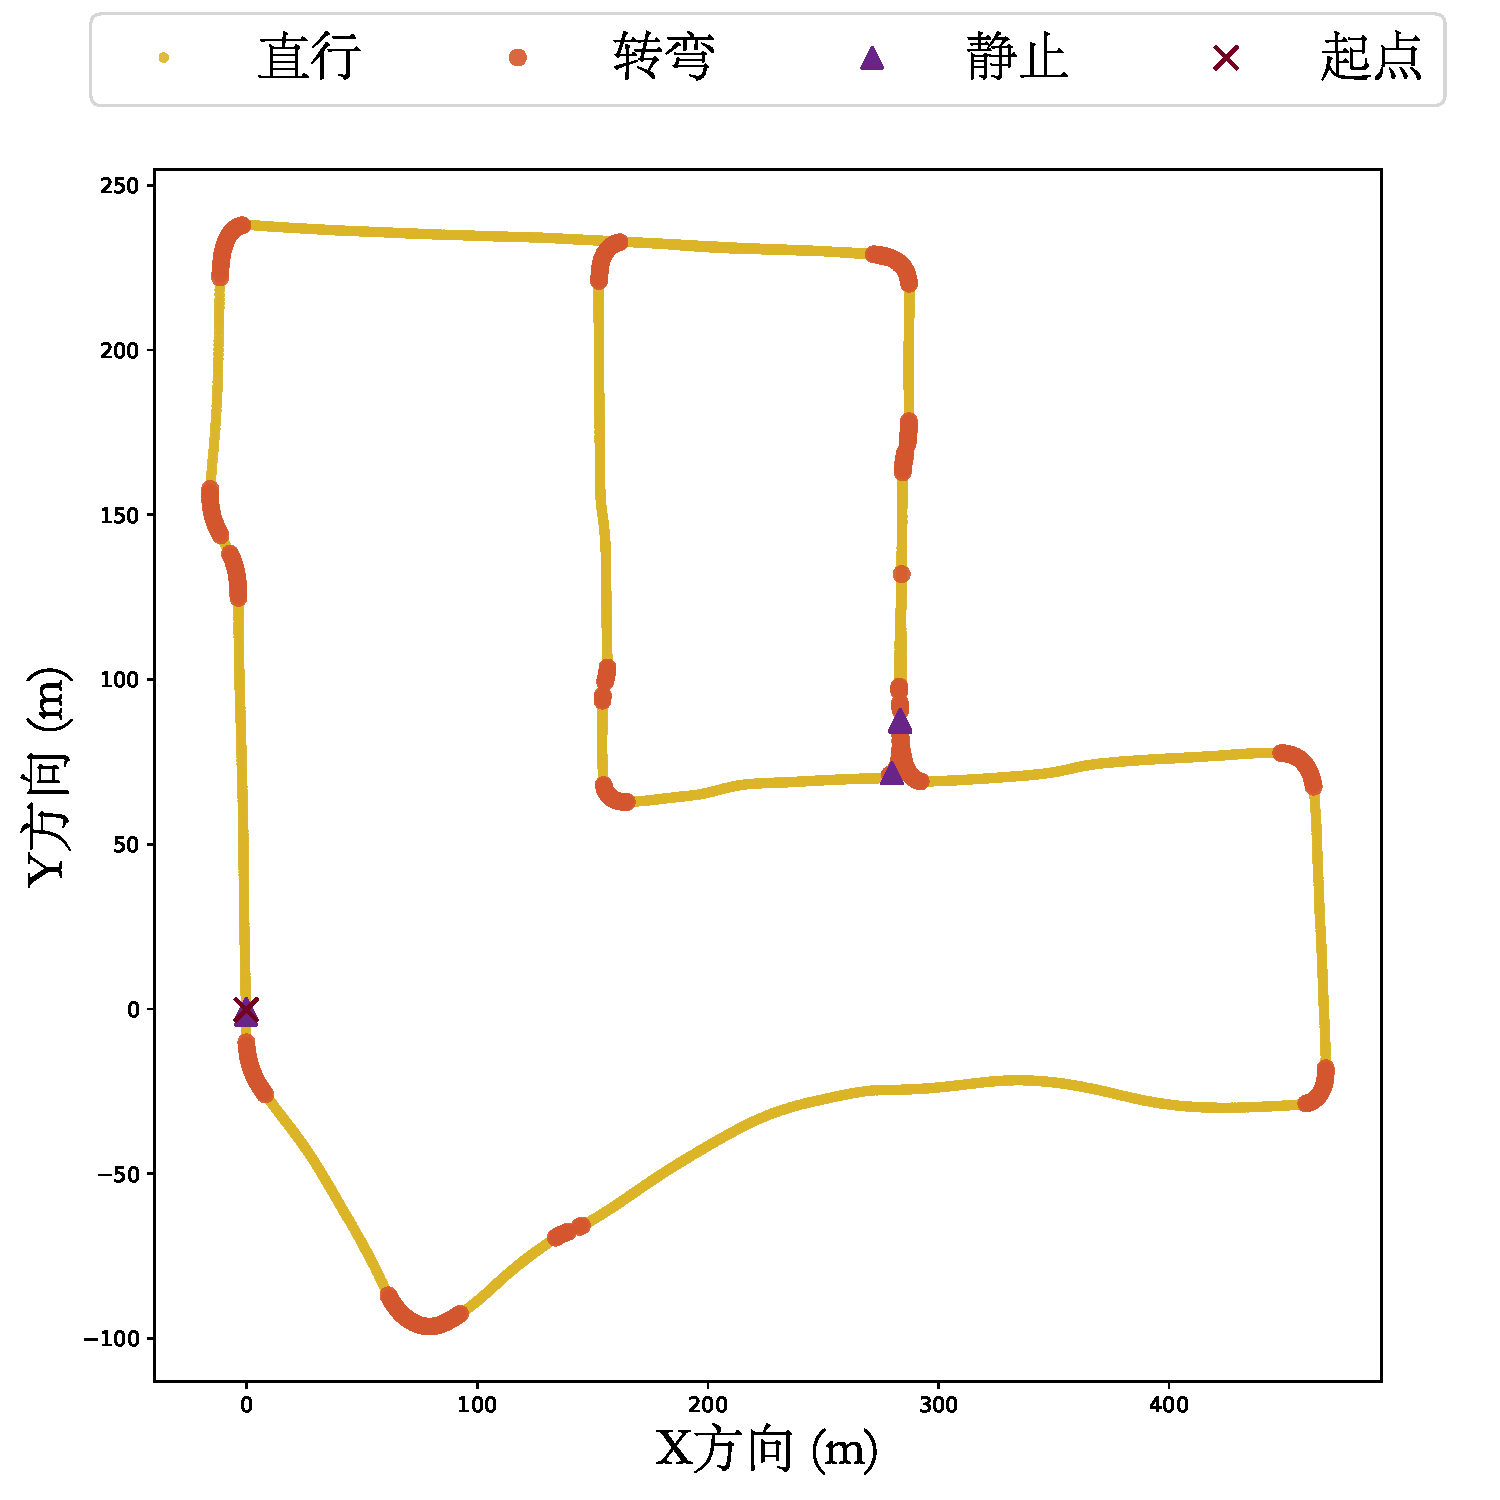
\includegraphics[width=0.47\linewidth]{distrib1.pdf}
  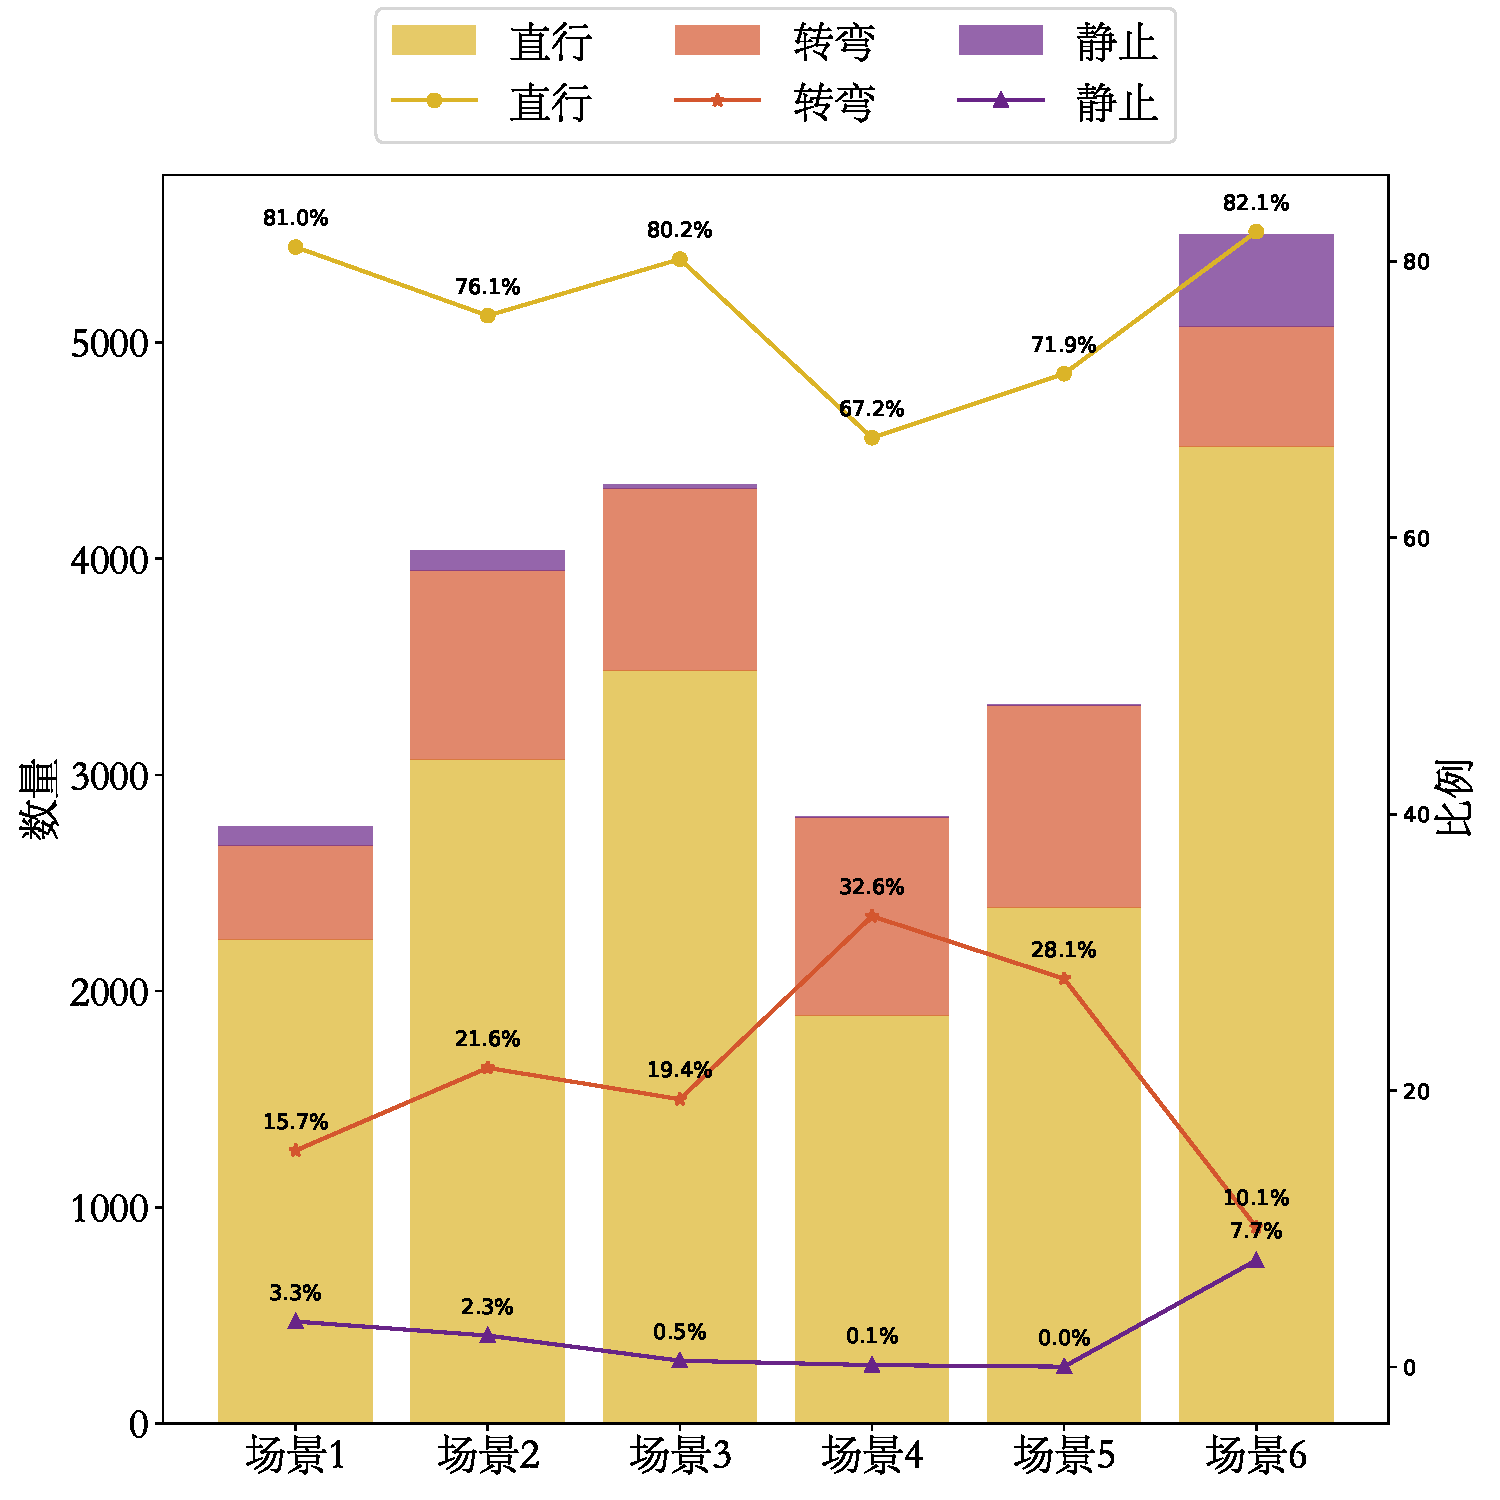
\includegraphics[width=0.47\linewidth]{hist.pdf}
  \caption{车身状态分布情况}
  \label{fig:data_distrib}
\end{figure}

在损失函数和训练策略方面,由于模型的最终输出会使用Sigmoid函数进行概率预测,相对应的损失函数选择二值交叉熵损失函数(Binary Cross Entropy, BCE)。在训练策略方面,本文使用Adam优化器\cite{kingma2014adam},学习率为$1e-4$,训练批次大小为8,训练轮数为100。此外,由于一般情况下车辆直行的情况比静止和转弯的情况要多,如图~\ref{fig:data_distrib}所示,因此如果直接使用全部数据训练,则会导致样本分布的不均衡。为了解决这个问题,本文在数据采样方面使用了均衡策略:在训练的每个epoch中,以转弯和静止区间的并集数据量为基准,从直行数据中随机采样等量数据,然后与转弯和静止区间的并集数据合并。

\section{伪观测预处理}

伪观测可以为视觉惯性里程计增加一定的约束条件,但是其并不能直接使用,而是需要一定的预处理过程,其中最关键的就是惯性-车体粗对齐。如图~\ref{fig:vehicle}中的坐标系示意图所示,车身坐标系和IMU体坐标系往往并不重合,有时甚至有较大的差距,而视觉惯性里程计中一般以IMU体坐标系作为姿态估计的基准坐标系。因此,如果使用车身坐标系的速度作为约束,就需要将车身坐标系的速度转换为IMU体坐标系的速度。这就需要进行惯性-车体粗对齐,即将车身坐标系的速度转换为IMU体坐标系的速度。一般来说,这个转换关系需要包含旋转和平移两种变换,但是考虑到车身整体的刚性结构,IMU与车身之间也是刚性连接,因此可以将车身坐标系与IMU体坐标系的原点等价为重合状态,在这种状态下可以只考虑车身坐标系与IMU坐标系之间的旋转关系。

在拥有状态判别,并且只考虑两坐标系之间旋转关系的情况下,求解车身坐标系和IMU体坐标系之间的关系还可以使用一些更强的先验知识:
\begin{enumerate}
  \item 在车辆直行的情况下,速度方向基本指向车身的前向,即车身坐标系的$y$轴;
  \item 在车辆直行的情况下,速度大小基本为合速度的模长。
\end{enumerate}
基于以上假设,可以使用以下方法求解车身坐标系和IMU体坐标之间的转换关系。

首先根据车身状态判别的结果,筛选直行时刻的IMU速度估计$\{\symbf{v}^o_{b_{j}}\}^n$,其中$\symbf{v}^o_{b_{j}}$表示第$j$时刻的IMU速度估计,$n$表示IMU速度估计的总数,然后使用视觉惯性里程计估计的车身姿态$\{ \symbf{R}_{b_{j}}^o\}^n$可以获得IMU体坐标系下的速度估计
\begin{equation}
  \{\symbf{v}^{b_{j}}\}^n = \{ {\symbf{R}_{b_{j}}^o}^{-1} \cdot \symbf{v}^o_{b_{j}} \}^n.
\end{equation}
又根据直线行驶时的车身假设可以获得此时车身坐标系下的速度为
\begin{equation}
  \{\symbf{v}^{v_{j}}\}^n = \{ \begin{bmatrix}
    0 \\
    || \symbf{v}^{b_{j}} || \\ 
    0
  \end{bmatrix}\}^n.
\end{equation}
此时,关于车体和IMU体坐标系之间的旋转关系$\symbf{R}_{b}^{v}$可以求解以下带有约束的优化问题获得:
\begin{equation}
\begin{aligned}
  &\min_{\symbf{R}_{b}^{v}} \symbf{J} = \frac{1}{2} \sum_{j=1}^{n} \| \symbf{v}^{v_{j}} - \symbf{R}_{b}^{v} \cdot \symbf{v}^{b_{j}} \|_2^2 \\
  \text{s.t.} & \quad {(\symbf{R}_{b}^{v})}^T \symbf{R}_{b}^{v} = \symbf{I}
\end{aligned},
\end{equation}
其中的约束条件是为了保证所求旋转矩阵是一个合法的旋转矩阵。针对上述优化问题,其求解过程如下:
\begin{equation}
\begin{aligned}
  2\symbf{J} &= \sum_{j=1}^{n} \| \symbf{v}^{v_{j}} - \symbf{R}_{b}^{v} \cdot \symbf{v}^{b_{j}} \|_2^2 \\ 
  &= \sum_{j=1}^{n} {(\symbf{v}^{v_{j}} - \symbf{R}_{b}^{v} \cdot \symbf{v}^{b_{j}})}^T \cdot {(\symbf{v}^{v_{j}} - \symbf{R}_{b}^{v} \cdot \symbf{v}^{b_{j}})} \\
  &= \sum_{j=1}^{n} {({\symbf{v}^{v_{j}}}^T - {\symbf{v}^{b_{j}}}^T \cdot {\symbf{R}_{b}^{v}}^T)} \cdot {(\symbf{v}^{v_{j}} - \symbf{R}_{b}^{v} \cdot \symbf{v}^{b_{j}})} \\
  &= \sum_{j=1}^{n} ({\symbf{v}^{v_{j}}}^T \cdot \symbf{v}^{v_{j}} - {\symbf{v}^{v_{j}}}^T \cdot \symbf{R}_{b}^{v} \cdot \symbf{v}^{b_{j}} - {\symbf{v}^{b_{j}}}^T \cdot {\symbf{R}_{b}^{v}}^T \cdot {\symbf{v}^{v_{j}}} + {\symbf{v}^{b_{j}}}^T \cdot {\symbf{R}_{b}^{v}}^T \cdot \symbf{R}_{b}^{v} \cdot \symbf{v}^{b_{j}})
\end{aligned},
\end{equation}
根据约束条件${(\symbf{R}_{b}^{v})}^T \symbf{R}_{b}^{v} = \symbf{I}$可得
\begin{equation}
\begin{aligned}
  2\symbf{J} &= \sum_{j=1}^{n} ({\symbf{v}^{v_{j}}}^T \cdot \symbf{v}^{v_{j}} - {\symbf{v}^{v_{j}}}^T \cdot \symbf{R}_{b}^{v} \cdot \symbf{v}^{b_{j}} - {\symbf{v}^{b_{j}}}^T \cdot {\symbf{R}_{b}^{v}}^T \cdot {\symbf{v}^{v_{j}}} + {\symbf{v}^{b_{j}}}^T \cdot \symbf{v}^{b_{j}}) \\ 
  &= \sum_{j=1}^{n} (|| \symbf{v}^{v_{j}} ||^2 - 2\cdot {\symbf{v}^{v_{j}}}^T \cdot \symbf{R}_{b}^{v} \cdot \symbf{v}^{b_{j}} + || \symbf{v}^{b_{j}} ||^2) \\
  &= \sum_{j=1}^{n} (|| \symbf{v}^{v_{j}} ||^2 + || \symbf{v}^{b_{j}} ||^2) - 2 \sum_{j=1}^{n} {\symbf{v}^{v_{j}}}^T \cdot \symbf{R}_{b}^{v} \cdot \symbf{v}^{b_{j}}
\end{aligned},
\end{equation}
可以观察到此时$\symbf{J}$的最小化与前一常数项无关,仅与后项带$\symbf{R}_b^v$的项有关,因此可以将$\symbf{J}$的最小化问题转化为最大化后一项,即
\begin{equation}
  \max_{\symbf{R}_{b}^{v}} \symbf{J}' = \sum_{j=1}^{n} {\symbf{v}^{v_{j}}}^T \cdot \symbf{R}_{b}^{v} \cdot \symbf{v}^{b_{j}}.
\label{eq:max}
\end{equation}
注意到
\begin{equation}
\begin{aligned}
  \sum_{j=1}^{n} {\symbf{v}^{v_{j}}}^T \cdot \symbf{R}_{b}^{v} \cdot \symbf{v}^{b_{j}} &= \text{trace}({\symbf{V}^{v}}^T \cdot \symbf{R}_{b}^{v} \cdot \symbf{V}^{b}) \\ 
  &= \text{trace}( \symbf{R}_{b}^{v} \cdot \symbf{V}^{b} \cdot {\symbf{V}^{v}}^T)
\end{aligned},
\label{eq:trace}
\end{equation}
其中$\symbf{V}^{b}, {\symbf{V}^{v}}^T$分别是$\{\symbf{v}^{b_{j}}\}^n,\{\symbf{v}^{v_{j}}\}^n$序列的协方差矩阵。对$\symbf{V}^{b} \cdot {\symbf{V}^{v}}^T$进行奇异值分解(Singular Value Decomposition, SVD)可以获得
\begin{equation}
  \symbf{V}^{b} \cdot {\symbf{V}^{v}}^T = \symbf{U} \cdot \symbf{\Sigma} \cdot \symbf{V}^T,
\end{equation}
因此可以对式~\ref{eq:trace}进行变换得到
\begin{equation}
\begin{aligned}
  \text{trace}( \symbf{R}_{b}^{v} \cdot \symbf{V}^{b} \cdot {\symbf{V}^{v}}^T) &= \text{trace}(\symbf{R}_{b}^{v} \cdot \symbf{U} \cdot \symbf{\Sigma} \cdot \symbf{V}^T) \\
  &= \text{trace}(\symbf{\Sigma} \cdot \symbf{V}^T \cdot \symbf{R}_{b}^{v} \cdot \symbf{U})
\end{aligned},
\label{eq:svd}
\end{equation}
其中$\symbf{V}^T \cdot \symbf{R}_{b}^{v} \cdot \symbf{U}$为三个正交矩阵的乘积,因此仍是一个正交矩阵,而$\symbf{\Sigma}$为对角矩阵。根据正交矩阵的性质可知其内部所有元素均小于1(因为正交矩阵的行列式为1),所以对于$\text{trace}(\symbf{\Sigma} \cdot \symbf{V}^T \cdot \symbf{R}_{b}^{v} \cdot \symbf{U})$来说,其取得最大值时即$\symbf{V}^T \cdot \symbf{R}_{b}^{v} \cdot \symbf{U}$为单位矩阵。结合式~\ref{eq:max},式~\ref{eq:trace},式~\ref{eq:svd}可知,最大化$\symbf{J}'$时即
\begin{equation}
  \symbf{R}_{b}^{v} = \symbf{V} \cdot \symbf{U}^T.
\end{equation}
此时获得的$\symbf{R}_{b}^{v}$可能会因为存在噪声等原因而并不精确,但此过程仅为粗对齐,所以精度误差有一定的容忍,后续在非线性优化部分仍会对此参数进行持续优化。

\section{非线性优化}
经过车身状态判别和惯性-车体粗对齐之后,还需要将伪观测相关的两个因子加入到VIO的窗口优化中,才能发挥伪观测约束对于整个系统的提升作用。由于伪观测约束是在原有视觉惯性里程计的优化项上添加,因此描述伪观测约束的相关因子,必须了解视觉惯性里程计的状态估计量及相关约束。

本文的视觉惯性里程计的估计量可以表示为
\begin{equation}
\begin{aligned}
  \mathcal{X} &= \begin{bmatrix} \symbf{x}_0, \symbf{x}_1, \dots, \symbf{x}_n, \symbf{x}_c^b, \symbf{q}_b^v, \lambda_0, \lambda_1, \dots, \lambda_m \end{bmatrix} \\
  \symbf{x}_k &= \begin{bmatrix} \symbf{p}_{b_{k}}^o, \symbf{v}_{b_{k}}^o, \symbf{q}_{b_{k}}^o, \symbf{b}_a, \symbf{b}_{\omega} \end{bmatrix} \\
  \symbf{x}_c^b &= \begin{bmatrix} \symbf{q}_{c}^b, \symbf{q}_{c}^b \end{bmatrix}
\end{aligned},
\end{equation}
其中$\symbf{x}_k$表示第$k$帧时刻的IMU姿态,$\symbf{x}_c^b$表示相机到IMU的外参,$\symbf{q}_b^v$表示IMU到车身的外参,$\lambda_k$表示第$k$帧相机的特征点深度。$\symbf{q}_b^v$是惯性-车体因子,其表示IMU体坐标系到车身坐标系的旋转关系。

根据以上的状态估计量,可以得到视觉惯性里程计的优化目标函数
\begin{equation}
  \min_{\mathcal{X}} \begin{Bmatrix} || \symbf{r}_p - \symbf{H}_p \cdot \mathcal{X} ||^2 + \sum_{k\in\mathcal{B}} || \symbf{r}_{\mathcal{B}}(\hat{\symbf{z}}_{b_k}^{b_{k+1}}, \mathcal{X}) ||^2_{\symbf{P}_{b_k}^{b_{k+1}}} + \sum_{(l,j)\in\mathcal{C}} \rho(|| \symbf{r}_{\mathcal{C}}(\hat{\symbf{z}}_{l}^{c_j}, \mathcal{X}) ||^2_{\symbf{P}_{l}^{c_j}}) \end{Bmatrix},
\end{equation}
其中$\symbf{r}_p, \symbf{H}_p$代表与边缘化相关的观测与矩阵,$\symbf{r}_{\mathcal{C}}$代表视觉观测的残差函数,$\symbf{r}_{\mathcal{B}}$是本文提出的、增加了伪观测约束的IMU残差函数,$\symbf{P}_{l}^{c_j}$代表视觉观测的协方差矩阵,$\symbf{P}_{b_k}^{b_{k+1}}$代表伪观测约束的协方差矩阵,$\symbf{r}'_{\mathcal{B}}$具体可以表示为
\begin{equation}
  \symbf{r}_{\mathcal{B}}(\hat{\symbf{z}}_{b_k}^{b_{k+1}}, \mathcal{X}) = 
  \begin{bmatrix} 
    \symbf{R}_o^{b_k} \cdot (\symbf{p}_{b_{k+1}}^o -\symbf{p}_{b_k}^o-\symbf{v}_{b_k}^o\cdot\Delta t_k + \frac{1}{2}\symbf{g}^o{\Delta t_k}^2) - \hat{\symbf{\alpha}}_{b_{k+1}}^{b_k} \\
    \symbf{R}_o^{b_k} \cdot (\symbf{v}_{b_{k+1}}^o - \symbf{v}_{b_k}^o + \symbf{g}^o\Delta t_k) - \hat{\symbf{\beta}}_{b_{k+1}}^{b_k} \\
    2[{\symbf{q}^o_{b_k}}^{-1}\otimes\symbf{q}_{b_{k+1}}^o \otimes \hat{\symbf{\gamma}}_{b_{k+1}}^{b_k}]_{xyz} \\
    \symbf{b}_{ab_{k+1}} - \symbf{b}_{ab_{k}} \\
    \symbf{b}_{\omega b_{k+1}} - \symbf{b}_{\omega b_{k}} \\
    \symbf{A} \cdot \symbf{R}_b^v \cdot {\symbf{R}_{b_k}^o}^{-1} \cdot \symbf{v}_{b_k}^o
  \end{bmatrix},
  \label{eq:imu_residual}
\end{equation}
其中$\Delta t_k$表示时间间隔,$\symbf{g}^o$表示VIO世界坐标系下的重力向量,$\hat{\symbf{\alpha}}_{b_{k+1}}^{b_k}, \hat{\symbf{\beta}}_{b_{k+1}}^{b_k}, \hat{\symbf{\gamma}}_{b_{k+1}}^{b_k}$分别表示相对位移、相对速度和相对旋转的预积分观测值,其具体表示参考Qin等\cite{qin2018vins}的工作。IMU残差函数的最后一项是相较于经典视觉惯性里程计而增加的速度伪观测约束。$A$是一个指示函数,其取值根据车身状态判别的结果取值
\begin{equation}
  A = 
  \begin{cases}
    \begin{bmatrix} \symbf{e_1}, \symbf{e_2}, \symbf{e_3}  \end{bmatrix}, \symbf{y}^{FOR} = 1 \\
    \begin{bmatrix} \symbf{0}, \symbf{e_2}, \symbf{e_3}  \end{bmatrix}, \symbf{y}^{LAT} = 1 \\
    \begin{bmatrix} \symbf{0}, \symbf{0}, \symbf{0}  \end{bmatrix}, \text{Otherwise}
  \end{cases}.
\end{equation}
其中$\symbf{e}_i$表示单位矩阵的第$i$列向量,$\symbf{y}^{FOR}, \symbf{y}^{LAT}$分别表示预测的车辆前进和横向的状态。

若使用伪观测约束,需要使用其相对于各估计量的雅可比矩阵。为了简化表达,本处使用$\symbf{r}'_{\mathcal{B}}$代表IMU残差函数中的伪观测约束,即式~\ref{eq:imu_residual}的最后一项。首先给出速度伪观测约束相对于状态量$\symbf{v}_{b_{k}}^o$的雅可比矩阵
\begin{equation}
  \frac{\partial \symbf{r}'_{\mathcal{B}}}{\partial \symbf{v}_{b_{k}}^o} = \symbf{A} \cdot \symbf{R}_b^v \cdot {\symbf{R}_{b_k}^o}^{-1}.
\end{equation}
对于$\symbf{q}_{b_{k}}^o$的雅可比矩阵,约束中并没有直接使用四元数$\symbf{q}_{b_{k}}^o$,而是使用等价的旋转矩阵$\symbf{R}_{b_{k}}^o$,避免了四元数运算$\otimes$的繁琐使用。求导方式本文选择使用扰动模型\cite{imu_preintegration}进行,假设旋转的扰动值为$\symbf{\varphi } \in \mathbb{R}^3$(对于四元数和旋转矩阵有同样的效果),则:
\begin{equation}
\begin{aligned}
  \frac{\partial \symbf{r}'_{\mathcal{B}}}{\partial \symbf{q}_{b_{k}}^o} &\triangleq  \frac{\partial \symbf{r}'_{\mathcal{B}}}{\partial \symbf{\varphi }} \\
  &= \lim\limits_{\symbf{\varphi } \to \symbf{0}} \frac{\symbf{A} \cdot \symbf{R}_b^v \cdot {\text{exp}(\symbf{\varphi }^{\land}) \cdot {\symbf{R}_{b_k}^o}^{-1}} \cdot \symbf{v}_{b_k}^o - \symbf{A} \cdot \symbf{R}_b^v \cdot {{\symbf{R}_{b_k}^o}^{-1}} \cdot \symbf{v}_{b_k}^o}{\symbf{\varphi }} \\
  &= \lim\limits_{\symbf{\varphi } \to \symbf{0}} \frac{\symbf{A} \cdot \symbf{R}_b^v \cdot {\text{exp}(\symbf{\varphi }^{\land}) \cdot \symbf{R}^{b_k}_o} \cdot \symbf{v}_{b_k}^o - \symbf{A} \cdot \symbf{R}_b^v \cdot {\symbf{R}^{b_k}_o} \cdot \symbf{v}_{b_k}^o}{\symbf{\varphi }} \\
  &= \lim\limits_{\symbf{\varphi } \to \symbf{0}} \frac{\symbf{A} \cdot \symbf{R}_b^v \cdot {[(\symbf{I} + \symbf{\varphi }^{\land}) \cdot \symbf{R}^{b_k}_o]} \cdot \symbf{v}_{b_k}^o - \symbf{A} \cdot \symbf{R}_b^v \cdot {\symbf{R}^{b_k}_o} \cdot \symbf{v}_{b_k}^o}{\symbf{\varphi }} \\
  &= \lim\limits_{\symbf{\varphi } \to \symbf{0}} \frac{\symbf{A} \cdot \symbf{R}_b^v \cdot {({\symbf{R}^{b_k}_o} + \symbf{\varphi }^{\land} \cdot \symbf{R}^{b_k}_o)} \cdot \symbf{v}_{b_k}^o - \symbf{A} \cdot \symbf{R}_b^v \cdot {\symbf{R}^{b_k}_o} \cdot \symbf{v}_{b_k}^o}{\symbf{\varphi }} \\
  &= \lim\limits_{\symbf{\varphi } \to \symbf{0}} \frac{\symbf{A} \cdot \symbf{R}_b^v \cdot {\symbf{\varphi }^{\land} \cdot \symbf{R}^{b_k}_o} \cdot \symbf{v}_{b_k}^o}{\symbf{\varphi }}
  = \lim\limits_{\symbf{\varphi } \to \symbf{0}} \frac{-\symbf{A} \cdot \symbf{R}_b^v \cdot ({\symbf{R}^{b_k}_o} \cdot \symbf{v}_{b_k}^{o})^{\land} \cdot \symbf{\varphi}}{\symbf{\varphi }} \\
  &= -\symbf{A} \cdot \symbf{R}_b^v \cdot ({\symbf{R}^{b_k}_o} \cdot \symbf{v}_{b_k}^{o})^{\land}
  = -\symbf{A} \cdot \symbf{R}_b^v \cdot ({\symbf{R}_{b_k}^o}^{-1} \cdot \symbf{v}_{b_k}^{o})^{\land}
\end{aligned},
\end{equation}
其中${\land}$表示将一个向量转换为反对称矩阵的函数,在推导中直接使用了近似
\begin{equation}
  \text{exp}(\symbf{\varphi }^{\land}) \approx \symbf{I} + \symbf{\varphi }^{\land}.
\end{equation}
和反对称矩阵的乘法交换规律
\begin{equation}
  \symbf{a}^{\land} \cdot \symbf{b} = -\symbf{b}^{\land} \cdot \symbf{a}.
\end{equation}
同理可得伪观测约束关于惯性-车体因子的雅可比矩阵:
\begin{equation}
  \frac{\partial \symbf{r}'_{\mathcal{B}}}{\partial \symbf{q}_{b_{k}}^o} = -\symbf{A} \cdot (\symbf{R}_b^v \cdot {\symbf{R}_{b_k}^o}^{-1} \cdot \symbf{v}_{b_k}^o)^{\land}.
\end{equation}
至此已经给出了速度伪观测对于估计量的雅可比矩阵。根据雅可比矩阵,使用高斯牛顿法或者列文伯格-马夸尔特法进行非线性优化,以获得最终的状态估计量。

\section{本章总结}
本章主要介绍了固定路线定位系统中的视觉惯性里程计设计。整体设计考虑了车辆或轮式机器人的特殊运动状态,首先借助深度学习技术对车辆的运动状态进行判别,这一部分包括了网络设计和详细的训练过程;然后根据判别结果进行伪观测预处理,这一部分主要是使用视觉惯性里程计本身估计的速度和假设的车身状态进行粗对齐;最后将伪观测约束和惯性-车体因子加入到视觉惯性里程计的非线性优化中,以提高定位的精度。
% !TeX root = ../thuthesis-example.tex

\chapter{紧耦合地图定位}


\externaldocument{chap02}
\externaldocument{chap03}
\externaldocument{chap04}


\chapter{视觉惯性定位系统搭建与测试}

本章主要对定位系统的搭建与测试进行介绍。首先介绍了定位系统运行所依靠的硬件平台以及软件环境:不同于一般的定位系统,本文方法的实施依赖于深度学习及图形处理单元(Graphics processing unit, GPU)。然后介绍了本章所使用的数据集以及评价指标。本章实验主要建立在3个数据集上:KITTI数据集、4Seasons数据集和KAIST数据集。其中KITTI数据集场景相对单一,适合验证离线建图模块的性能,以及初步验证定位模块的性能;4Seasons数据集提供的场景丰富,适合验证VIO和紧耦合地图定位模块的性能;KAIST数据集提供了超长轨迹,适合验证VIO模块的性能。最后本章介绍了定位系统三个模块的测试结果,并通过相应的消融实验和效率测试来验证各部分的真实作用和可行性。

\section{系统与测试细节}
\subsection{硬件与软件环境}

本文所设计的定位系统的运行环境依赖于同时具有CPU(Central Processing Unit)和GPU(Graphics Processing Unit)的计算机,具体来说本文的实验平台使用12th Gen Intel Core i7-12700 CPU和NVIDIA GeForce RTX 3080 GPU。

系统的软件部署环境如图~\ref{fig:software} 所示,其中Ubuntu 20.04 LTS是本章所使用的操作系统;ROS Noetic是本章所使用的机器人操作系统,其主要作用是将多个子系统的结果方便快捷地统一处理;VINS-Mono是本章所使用的视觉惯性定位系统的基线,其具有较为简洁的逻辑划分,方便快速改进、验证想法;TensorRT是本章所使用的深度学习推理框架,其主要负责系统中的神经网络推理任务,其针对NVIDIA显卡的速度优化使得整个系统可以实时运行。此外,本文所设计系统中还有大量超参数,其具体取值如表~\ref{tab:hyperparameters} 所示。

\begin{figure}
  \centering
  \subcaptionbox{Ubuntu 20.04}{
\includegraphics[width=0.22\linewidth]{ubuntu_logo.png}}
  \subcaptionbox{ROS Noetic}{
\includegraphics[width=0.18\linewidth]{noetic_logo.png}}
  \subcaptionbox{VINS-Mono}{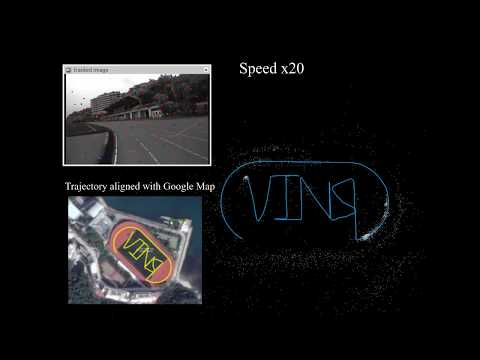
\includegraphics[width=0.22\linewidth]{VINS_logo.jpeg}}
  \subcaptionbox{TensorRT}{
\includegraphics[width=0.3\linewidth]{tensorrt_logo.png}}
  \caption{软件部署环境}
  \label{fig:software}
\end{figure}

\begin{table}
\centering
\caption{实验中所涉及的本文系统运行超参数}
\setlength{\tabcolsep}{6mm}{
\begin{tabular}{lccc}
\toprule
参数名 & 首次出现章节 & 作用 & 取值 \\
\midrule
$t_l$ & \ref{sec:map_sfm} & SfM中回环检测相似度阈值 & 0.8 \\
$m$ & \ref{sec:map_sfm} & SfM中回环帧数量 & 5 \\
$\alpha$ &  \ref{sec:map_fusion}  & 建图融合GNSS观测权重系数     & 1000 \\
$\tau$ & \ref{sec:network_design} & 车辆状态正例预测阈值 & 0.9 \\
$N_c$ & \ref{sec:loc_vote}  & 粗到细匹配候选关键帧数量 & 7   \\
$t_r$ &  \ref{sec:loc_vote}  & 投票过程相对旋转角度阈值 & $15\degree$   \\
$t_p$ &  \ref{sec:loc_vote}  & 投票过程相对位移阈值   & 5m    \\
$\lambda_r$ &  \ref{sec:valid}  & 有效性验证角度阈值    & $60\degree$   \\
$\lambda_p$ &  \ref{sec:valid}  & 有效性验证位移阈值    & 15m   \\
$N$ &  \ref{sec:loc_pg}  & 滑动窗口容量       & 20   \\
$\kappa$ &  \ref{sec:loc_pg}  & 单帧图像所考虑的点云比例 & 10  \\
\bottomrule
\end{tabular}}
\label{tab:hyperparameters}
\end{table}

\subsection{测试数据集与评价指标}
\subsubsection{KITTI数据集}
KITTI 数据集\cite{Geiger2012CVPR}是SLAM和自动驾驶研究中最受欢迎且使用广泛的数据集之一,它包含大量的多种传感器采集的交通场景数据,如图~\ref{fig:kitti_data} 展示,包括高分辨率RGB双目相机图像、灰度双目相机图像以及3D激光雷达数据。该数据集提供了11条经过精心选择的序列,构成视觉里程计基准。每条序列包含来自四个相机的数据:两个灰度相机和两个彩色相机。此外,KITTI 数据集还为这11条视觉里程计基准序列中的10条提供了原始GNSS观测数据和IMU测量数据。

\begin{figure}
  \centering
  \subcaptionbox{序列00-城镇环境}{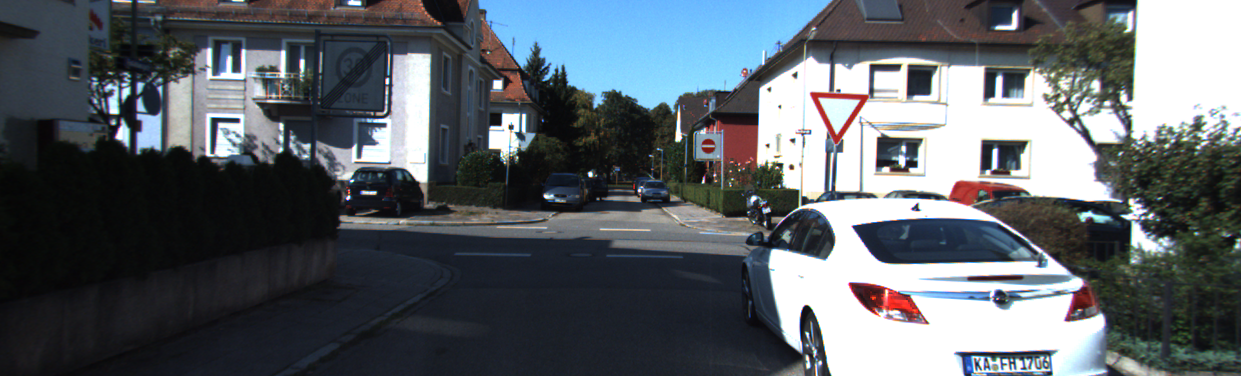
\includegraphics[width=0.47\linewidth]{kitti_00.png}}
  \subcaptionbox{序列01-高架环境}{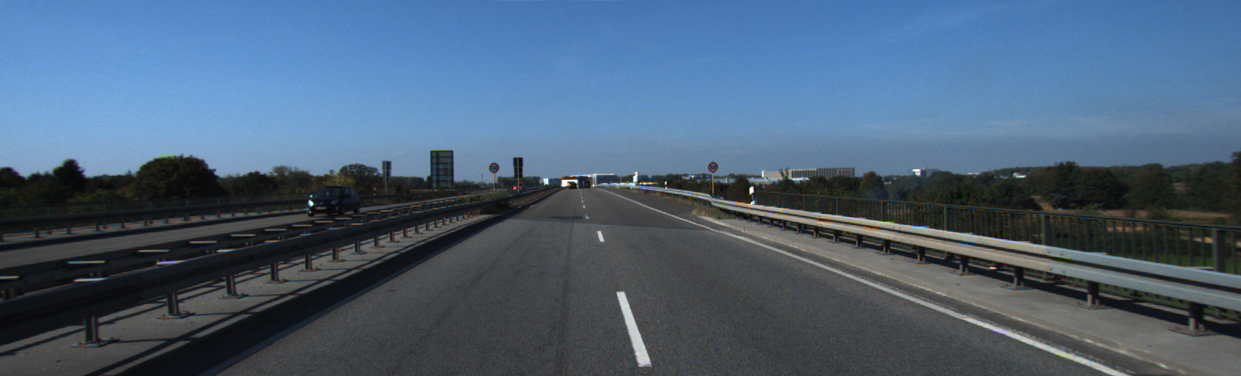
\includegraphics[width=0.47\linewidth]{kitti_01.png}}
  \subcaptionbox{序列09-郊外环境}{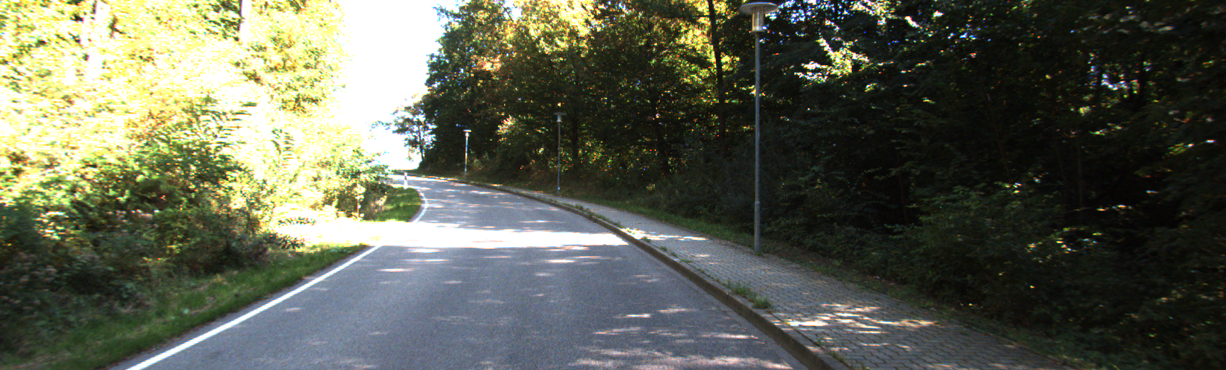
\includegraphics[width=0.47\linewidth]{kitti_09.png}}
  \subcaptionbox{序列10-农村环境}{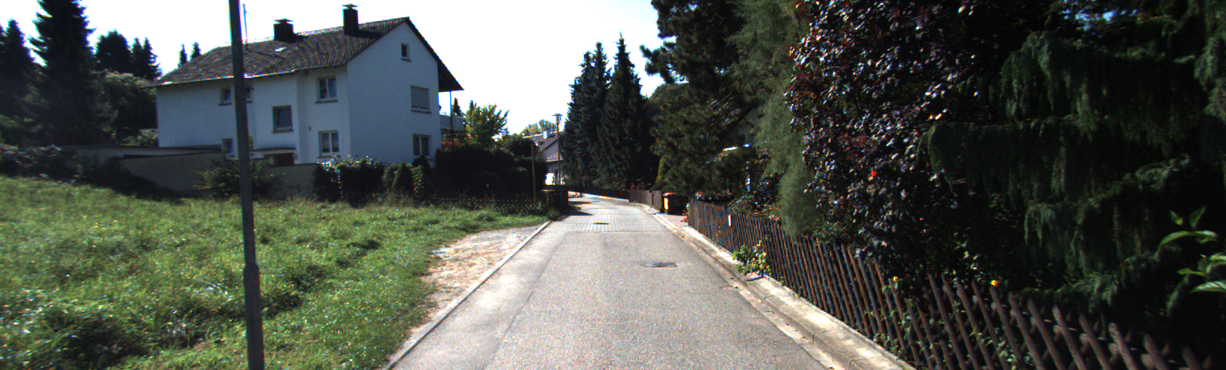
\includegraphics[width=0.47\linewidth]{kitti_10.png}}
  \caption{KITTI数据集场景}
  \label{fig:kitti_data}
\end{figure}

本章使用KITTI视觉里程计基准中包含GNSS观测数据的10条序列,评估本章所提出系统的建图性能以及整体性能。这10条序列包括了城镇、高架、郊外以及农村等常见的车辆行驶环境。

\subsubsection{4Seasons数据集}
4Seasons数据集\cite{wenzel20214seasons}是一个专为自动驾驶研究设计的数据集,提供了涵盖季节变化和复杂感知条件的图像、IMU等数据。同一路径在不同季节和多种感知条件下被多次采集,使其特别适合于评估针对固定路径设计的方法。该数据集使用的传感器包括立体相机、IMU和RTK-GNSS,同时还提供了精度达到厘米级的高精度真值位姿。

与KITTI数据集相比,4Seasons数据集能够提供更具挑战性和说服力的实验结果,突出了本文方法的优势。本章选择了四个具有代表性的场景,分别是

\textbf{(1)Office Loop(OF):} 位于城郊工业区的环形路线,长度约为3776米,包含了多种感知条件,如建筑物、树木和道路标志等,如图~\ref{fig:OF_data} 所示。此路线在不同季节采集了5条序列(以OF1-5代称),每条序列包含了来自灰度立体相机、IMU和RTK-GNSS的数据。
\begin{figure}
  \centering
  \subcaptionbox{场景感知条件}{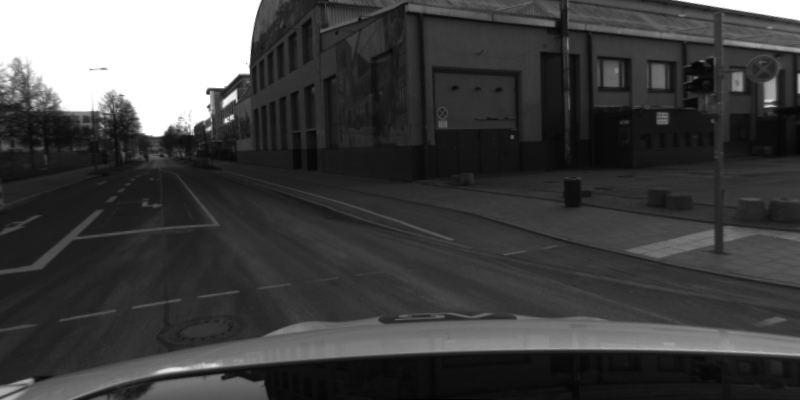
\includegraphics[width=0.48\linewidth]{OfficeLoop.png}}
  \subcaptionbox{路径卫星图}{\includegraphics[width=0.48\linewidth]{gnss_OF1.png}}
  \caption{Office Loop场景}
  \label{fig:OF_data}
\end{figure}

\textbf{(2) Neighborhood(NH):} 位于城镇环境的环形路线,长度约为2106米,包含了多种感知条件,如树木和房屋等,包含了更多的植被,接近于农村环境,如图~\ref{fig:NH_data} 所示。此路线在不同季节采集了7条序列(以NH1-7代称),每条序列包含了来自灰度立体相机、IMU和RTK-GNSS的数据。

\begin{figure}
  \centering
  \subcaptionbox{场景感知条件}{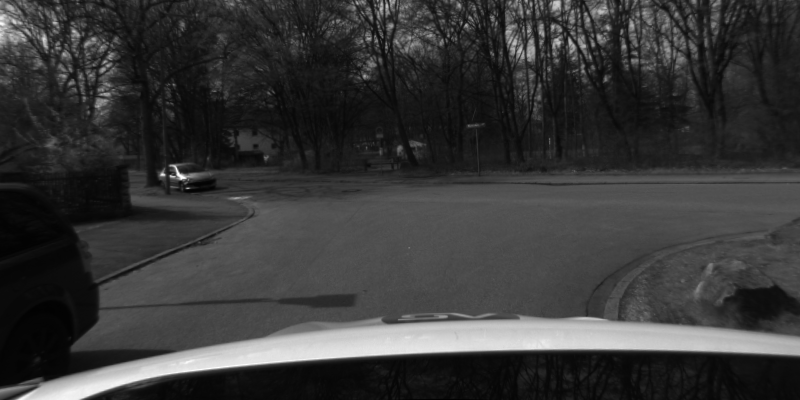
\includegraphics[width=0.48\linewidth]{Neighborhood.png}}
  \subcaptionbox{路径卫星图}{\includegraphics[width=0.48\linewidth]{gnss_NH01.png}}
  \caption{Neighborhood场景}
  \label{fig:NH_data}
\end{figure}

\textbf{(3)Business Campus(BC):} 位于校园和商业区的多条环形路线,长度约为3011米,包含了更多的建筑物,如图~\ref{fig:BC_data} 所示。此路线在不同季节采集了3条序列(以BC1-3代称),每条序列包含了来自灰度立体相机、IMU和RTK-GNSS的数据。

\begin{figure}
  \centering
  \subcaptionbox{场景感知条件}{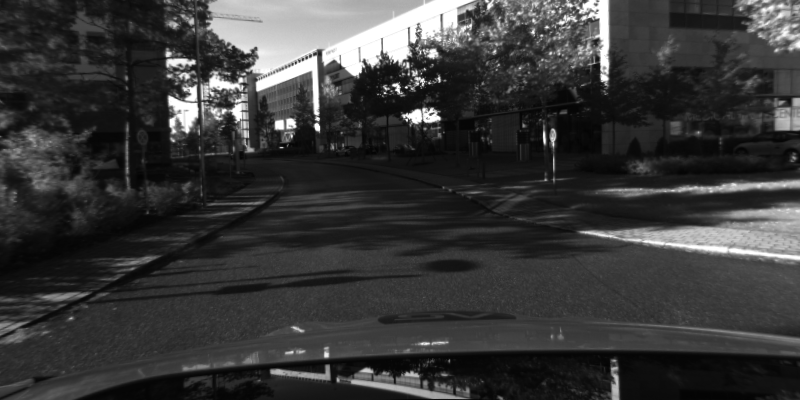
\includegraphics[width=0.48\linewidth]{BusinessCampus.png}}
  \subcaptionbox{路径卫星图}{\includegraphics[width=0.48\linewidth]{gnss_BC1.png}}
  \caption{Business Campus场景}
  \label{fig:BC_data}
\end{figure}

\textbf{(4)Old Town(OT):} 位于城市中心的商业区环线,长度约为5034米,包含了多种感知条件,此外还有大量的移动物体,如汽车、行人和自行车等,如图~\ref{fig:OT_data} 所示。此路线在不同季节采集了2条序列(以OT1-2代称),每条序列包含了来自灰度立体相机、IMU和RTK-GNSS的数据。

\begin{figure}
  \centering
  \subcaptionbox{场景感知条件}{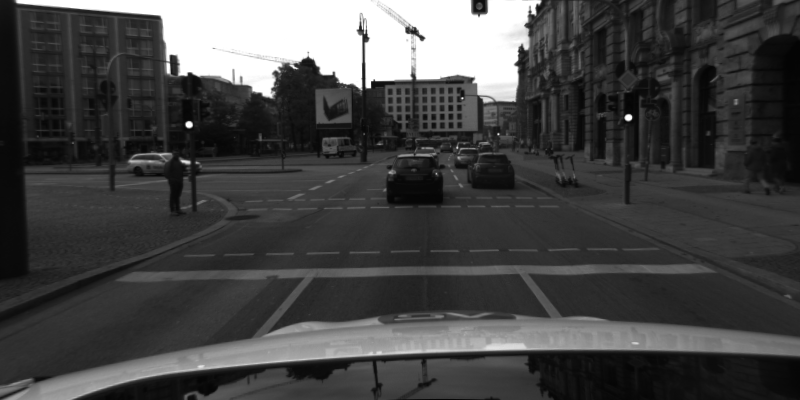
\includegraphics[width=0.48\linewidth]{OldTown.png}}
  \subcaptionbox{路径卫星图}{\includegraphics[width=0.48\linewidth]{gnss_OT1.png}}
  \caption{Old Town场景}
  \label{fig:OT_data}
\end{figure}

\subsubsection{KAIST数据集}
KAIST数据集\cite{jjeong-2019-ijrr}同时提供了LiDAR(Light Detection And Ranging)、立体相机、GPS、IMU、编码器和气压计等多种传感器数据,使得研究者可以针对不同传感器组合进行多模态信息处理。采集环境涵盖了从多车道宽阔道路到高密度城市街区等多种复杂场景,这不仅体现了实际城市环境中GPS信号不稳定、遮挡严重等问题,也为算法在动态、遮挡等极端条件下的鲁棒性验证提供了真实数据。此外,数据集通过高精度传感器与消费者级传感器的双层数据采集,以及精细的时间同步和标定处理,确保了数据的高准确性和一致性,并提供了基准轨迹及ROS工具,极大地方便了机器人定位、SLAM及环境感知等相关领域的研究与测试。

本章中主要选择了KAIST数据集中的三个场景,分别是20-Highway、26-Dongtan和28-Pangyo,如图~\ref{fig:KAIST_data} 所示。这三个场景分别代表了高速公路、郊区和城市环境,适合于测试本文方法在不同场景下的性能。其中28-Pangyo是一段超过10公里的城市环境,包含了大量的建筑物、行人和车辆,是一个非常具有挑战性的场景。KAIST数据集主要被使用来评估本文的PO-VIO模块性能。

\begin{figure}
  \centering
  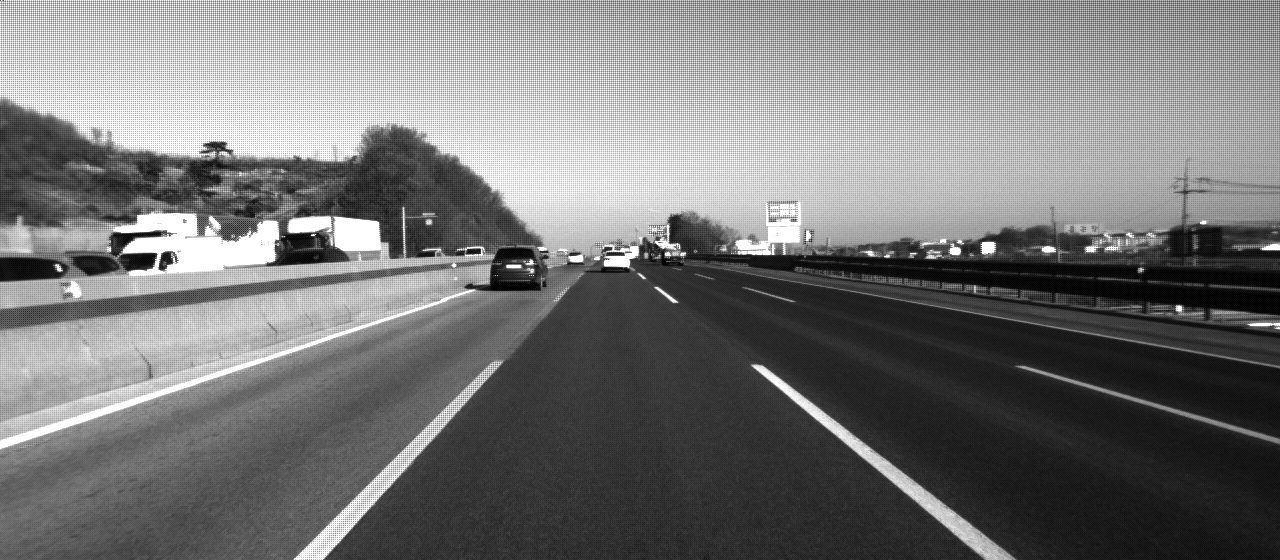
\includegraphics[width=0.32\linewidth]{KAIST_20_scene.png}
  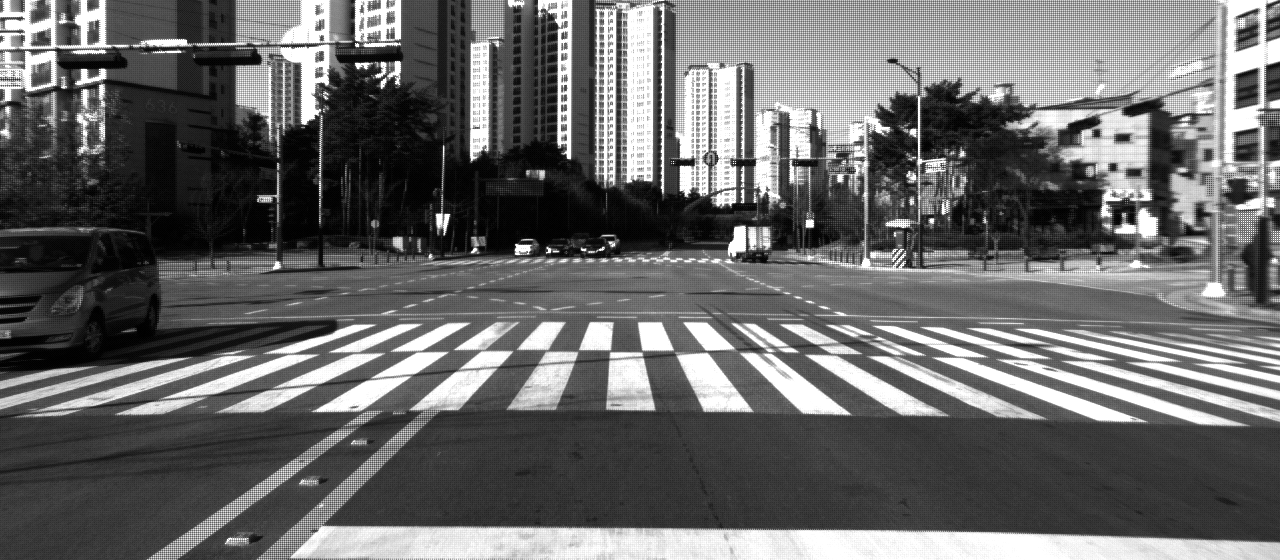
\includegraphics[width=0.32\linewidth]{KAIST_26_scene.png}
  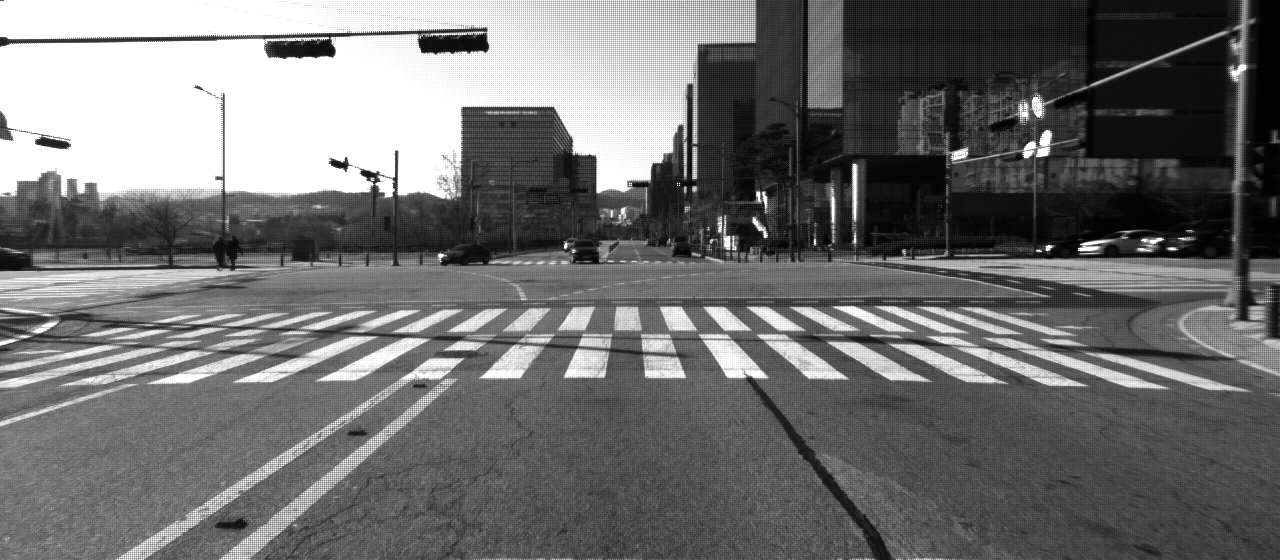
\includegraphics[width=0.32\linewidth]{KAIST_28_scene.png}
  \subcaptionbox{序列20-Highway}{\includegraphics[width=0.32\linewidth]{KAIST_20.png}}
  \subcaptionbox{序列20-Dongtan}{\includegraphics[width=0.32\linewidth]{KAIST_26.png}}
  \subcaptionbox{序列20-Pangyo}{\includegraphics[width=0.32\linewidth]{KAIST_28.png}}
  \caption{KAIST数据集场景}
  \label{fig:KAIST_data}
\end{figure}

\subsubsection{数据集使用划分}

由于本章需要分别验证3个模块的效果,因此本章将数据集的划分总结如表~\ref{tab:dataset_usage} 所示。表中的每一列代表了一个测试模块,每一行代表了一个数据集,表中的符号代表了数据集的使用方法,其中{\color[HTML]{3166FF} $\bigcirc$}代表使用该序列进行训练或者建图,{\color[HTML]{FD6864}$\bigtriangleup$}代表使用该序列进行测试。

\begin{table}
\centering
\begin{threeparttable}
\caption{数据集使用划分}
\setlength{\tabcolsep}{3.2mm}{
\begin{tabular}{lccccccc}
\toprule
\multirow{2}{*}{测试模块} & \multicolumn{2}{c}{KITTI}               & \multicolumn{4}{c}{4Seasons}   & KAIST                                         \\ \cline{2-8} 
                  & 灰色                          & 彩色         & OF1              & OF2-5            & \begin{tabular}[c]{@{}c@{}}NH1 \\ BC1 \\ OT1\end{tabular} & \begin{tabular}[c]{@{}c@{}}NH2-7 \\ BC2-3 \\ OT2-3\end{tabular} & \begin{tabular}[c]{@{}c@{}}20-Highway  \\ 26-Dongtan \\ 28-Pangyo\end{tabular} \\ \midrule
离线建图模块 & {\color[HTML]{3166FF} $\bigcirc$}{\color[HTML]{FD6864}$\bigtriangleup$} &            &                  &                  &               &         &          \\
PO-VIO模块           &                             &            & {\color[HTML]{FD6864}$\bigtriangleup$} & {\color[HTML]{FD6864}$\bigtriangleup$} & {\color[HTML]{3166FF} $\bigcirc$}    &         &     {\color[HTML]{FD6864}$\bigtriangleup$}     \\
地图定位模块           & {\color[HTML]{FD6864}$\bigtriangleup$}           & {\color[HTML]{3166FF} $\bigcirc$} & {\color[HTML]{3166FF} $\bigcirc$}       & {\color[HTML]{FD6864}$\bigtriangleup$} & {\color[HTML]{3166FF} $\bigcirc$}    & {\color[HTML]{FD6864}$\bigtriangleup$} & \\ \bottomrule
\end{tabular}}
\label{tab:dataset_usage}
\begin{tablenotes}
  \item [a] {\color[HTML]{3166FF} $\bigcirc$} 代表使用该序列进行训练或者建图。
  \item [b] {\color[HTML]{FD6864}$\bigtriangleup$} 代表使用该序列进行测试。
\end{tablenotes}
\end{threeparttable}
\end{table}

KITTI数据集参与离线建图和地图定位两个模块的测试:在评估建图过程时,使用来自单目灰度相机的完整图像集;在评估整体性能时由于KITTI数据集未直接提供沿同一路径的多次行驶数据,本章中通过使用不同的相机模拟多次行驶。具体而言,使用部分彩色相机拍摄的图像进行离线建图过程,然后使用灰度相机拍摄的图像测试紧耦合地图定位的精度。建图图像的比例设置为0.25,即只使用四分之一的彩色图像来构建先验地图,并在完整的灰度图像集上进行定位。

4Seasons数据集参与PO-VIO和地图定位两个模块的测试:在评估PO-VIO模块时,使用NH1、BC1和OT1的数据作为训练数据,OF1-5作为测试数据;在评估地图定位性能时,使用OF1、NH1、BC1和OT1作为建图数据,OF2-5、NH2-7、BC2-3和OT2-3作为测试数据。此外由于地图定位模块需要使用PO-VIO结果,而PO-VIO的训练数据与地图定位的测试数据没有重合,所以可以直接使用PO-VIO的结果作为紧耦合地图定位的输入而不需要担心训练数据中混入了测试数据。

KAIST数据集参与PO-VIO模块的测试:使用序列20-Highway、26-Dongtan和28-Pangyo作为测试数据,而此处的车身状态判别神经网络则直接使用4Seasons数据集上的预训练参数。

\subsubsection{评价指标}

本章实验中使用绝对轨迹误差(Absolute Translation Error, ATE)\cite{sturm2012benchmark}和相对位姿误差(Relative Pose Error, RPE)\cite{geiger2012we}来评估定位性能。其中绝对轨迹误差只评估位移分量,记做$ATE_t$,单位为“米”(m);相对位姿误差评估了相对平移和相对旋转的误差,分别记做$RPE_{t}$和$RPE_{r}$,单位分别为“米/100米”(m/100m)和“度/100米”($\degree$/100m),$RPE_{t}$的计算是在每100米的间隔中计算当前定位结果与真值(Ground Truth)的平移误差,$RPE_{r}$的计算是在每100米的间隔中计算当前定位结果与真值之间的旋转角度误差。

$ATE_t$的计算方式为可以表示为:
\begin{equation}
  ATE_t = \sqrt{\frac{1}{N}\sum_{i=1}^{N}\|\text{trans}(\symbf{T}_{gt,i}^{-1}\cdot \symbf{T}_{est,i})\|^{2}_{2}},
\end{equation}
其中$\text{trans}(\cdot)$表示提取转换矩阵的平移部分,$\symbf{T}_{gt,i}, \symbf{T}_{est,i}$分别表示位姿的真值和预测值。由于绝对轨迹误差的计算对于坐标系的选择较为敏感,因此每次计算前会首先使用Umeyama算法\cite{arun1987least}将估计的轨迹与真值轨迹对齐。

$RPE_{t}$和$RPE_{r}$的计算方式分别为:
\begin{align}
  RPE_{t} &= \sqrt{\frac{1}{|\mathcal{S}|}\sum_{(i,j) \in \mathcal{S}}\| \text{trans}\left ((\symbf{T}_{gt,j}^{-1} \cdot \symbf{T}_{gt,i})^{-1}\cdot (\symbf{T}_{est,j}^{-1} \cdot \symbf{T}_{est,i}) \right ) \|_2^2} \\
  RPE_{r} &= \sqrt{\frac{1}{|\mathcal{S}|}\sum_{(i,j) \in \mathcal{S}}\| \text{rot}\left ((\symbf{T}_{gt,j}^{-1} \cdot \symbf{T}_{gt,i})^{-1}\cdot (\symbf{T}_{est,j}^{-1} \cdot \symbf{T}_{est,i}) \right ) \|_2^2},
\end{align}
其中$\text{rot}(\cdot)$表示提取转换矩阵的旋转部分,$\mathcal{S}$表示相对位姿误差计算的间隔为100米的两帧集合,数值计算前使用Li等\cite{li2023textslam}提出的方法对估计轨迹与真值轨迹对齐。

选择ATE与RPE作为评估指标,是当前SLAM和VIO研究中广泛接受且标准化的评估方案:ATE衡量估计轨迹与真实轨迹之间的位置偏差,能够反映整个系统在地图构建或全局定位中的累积误差;RPE侧重于系统在两个时刻之间的相对变换误差,反映了算法对帧间运动的建模与估计能力;此外当系统存在跳变、漂移、跟踪失败等问题时,RPE更容易反映出其在某一段时间内的性能不稳定。因此,本章选择同时汇报这两类指标,以确保对系统性能的全面评估。

% 相对位姿误差的计算方式更加追求描述相对变换,能更好反映出里程计的性能。此外相对位姿误差的计算方式对于坐标系的选择不如绝对轨迹误差敏感,但也有一定要求,本章使用Lin等\cite{li2023textslam}提出的方法首先对估计的轨迹与真值轨迹对齐,然后再计算相应数值。

% 在实验结果汇报中,由于KITTI数据集提供的真值格式与其他数据集不同,所以在计算方法中,KITTI由官方提供的计算工具进行计算,数值精度最高保留2位小数;4Seasons和KAIST数据集上的实验结果则使用Grupp等\cite{grupp2017evo}提出的开源工具包EVO进行计算,精度相对较高,可以保留6位小数,方便更精确的对比。

\section{离线建图模块测试}
对于离线建图模块的性能测试,本节以地图关键帧的位姿评估来定量对比建图精度,实验中选择了KITTI数据集的所有序列来评估本文的建图方法以及其他几种建图方法,并使用三种指标进行对比,对比方法包括GNSS测量值、COLMAP~\cite{schonberger2016structure}、VINS-Stereo~\cite{qin2019a} 以及本文的离线建图方法。建图结果如表~\ref{tab:map_ate} 和表~\ref{tab:map_rpe} 所示。

\begin{table}
\centering
\begin{threeparttable}
\caption{多种建图方式在KITTI数据集上的$ATE_t$\textdownarrow{}对比}
\setlength{\tabcolsep}{5mm}
\begin{tabular}{lcccc}
\toprule
序列 & GNSS(上限) & COLMAP*\cite{schonberger2016structure} & VINS-Stereo\cite{qin2019a} & 离线建图          \\ \midrule
00 & 0.03 & 5.61   & 5.95   & \cellcolor[HTML]{FFCCC9}\textbf{0.33} \\
01 & 0.06 & N/A    & 6.49   & \cellcolor[HTML]{FFCCC9}\textbf{0.17} \\
02 & 0.03 & N/A    & 5.99   & \cellcolor[HTML]{FFCCC9}\textbf{0.61} \\
04 & 0.02 & 4.99   & 1.08   & \cellcolor[HTML]{FFCCC9}\textbf{0.54} \\
05 & 0.02 & 8.28   & 5.98   & \cellcolor[HTML]{FFCCC9}\textbf{0.24} \\
06 & 0.04 & 1.78   & 3.48   & \cellcolor[HTML]{FFCCC9}\textbf{1.55} \\
07 & 0.03 & 3.41   & 2.41   & \cellcolor[HTML]{FFCCC9}\textbf{0.20} \\
08 & 0.02 & N/A    & 3.85   & \cellcolor[HTML]{FFCCC9}\textbf{0.71} \\
09 & 0.03 & 8.50   & 1.78   & \cellcolor[HTML]{FFCCC9}\textbf{0.50} \\
10 & 0.03 & N/A    & 3.78   & \cellcolor[HTML]{FFCCC9}\textbf{0.79} \\ \bottomrule
\end{tabular}
\label{tab:map_ate}
\begin{tablenotes}
  \item [a] 星号*表示COLMAP的结果经过了尺度调整。
  \item [b] VINS-Stereo表示VINS-Fusion的双目版本,使用双目图片和GNSS测量。
\end{tablenotes}
\end{threeparttable}
\end{table}

% Please add the following required packages to your document preamble:
% \usepackage{multirow}
\begin{table}
\centering
\begin{threeparttable}
\caption{多种建图方式在KITTI数据集上的RPE\textdownarrow{}对比}
\begin{tabular}{lcccccc}
\toprule
\multirow{2}{*}{序列} & \multicolumn{3}{c}{$RPE_t \downarrow$}              & \multicolumn{3}{c}{$RPE_r\downarrow$}                    \\ \cline{2-7} 
                    & COLMAP & VINS-Stereo & 离线建图          & COLMAP       & VINS-Stereo & 离线建图  \\
\midrule
00                  & 1.91    & 3.45        & \cellcolor[HTML]{FFCCC9}\textbf{1.20} & 0.82          & 1.45        & \cellcolor[HTML]{FFCCC9}\textbf{0.69} \\
01                  & N/A     & 12.18       & \cellcolor[HTML]{FFCCC9}\textbf{0.84} & N/A           & 3.54        & \cellcolor[HTML]{FFCCC9}\textbf{0.13} \\
02                  & N/A     & 2.65        & \cellcolor[HTML]{FFCCC9}\textbf{0.63} & N/A           & 1.26        & \cellcolor[HTML]{FFCCC9}\textbf{0.27} \\
04                  & 4.12    & 2.71        & \cellcolor[HTML]{FFCCC9}\textbf{0.71} & \cellcolor[HTML]{FFCCC9}\textbf{0.11} & 0.62        & 0.14          \\
05                  & 1.75    & 1.41        & \cellcolor[HTML]{FFCCC9}\textbf{1.10} & 0.22          & 0.69        & \cellcolor[HTML]{FFCCC9}\textbf{0.19} \\
06                  & 1.37    & 1.33        & \cellcolor[HTML]{FFCCC9}\textbf{0.86} & 0.20          & 0.72        & \cellcolor[HTML]{FFCCC9}\textbf{0.17} \\
07                  & 1.16    & 1.17        & \cellcolor[HTML]{FFCCC9}\textbf{0.39} & 0.26          & 0.87        & \cellcolor[HTML]{FFCCC9}\textbf{0.24} \\
08                  & N/A     & 3.46        & \cellcolor[HTML]{FFCCC9}\textbf{1.87} & N/A           & 1.77        & \cellcolor[HTML]{FFCCC9}\textbf{1.17} \\
09                  & 0.86    & 4.45        & \cellcolor[HTML]{FFCCC9}\textbf{0.62} & 0.31          & 1.87        & \cellcolor[HTML]{FFCCC9}\textbf{0.25} \\
10                  & N/A     & 2.38        & \cellcolor[HTML]{FFCCC9}\textbf{0.68} & N/A           & 0.94        & \cellcolor[HTML]{FFCCC9}\textbf{0.19} \\ \bottomrule
\end{tabular}
\label{tab:map_rpe}
\begin{tablenotes}
  \item [a] 星号*表示COLMAP的结果经过了尺度调整。
  \item [b] VINS-Stereo表示VINS-Fusion的双目版本,使用双目图片和GNSS测量。
\end{tablenotes}
\end{threeparttable}
\end{table}

表中使用粗体和红底标出非GNSS观测值中的最佳性能结果,GNSS观测值可被视为位置建图精度的上限。此外,由于GNSS测量值仅提供平移信息而不包含旋转,实验仅在$ATE_t$指标下与GNSS测量值进行对比。

COLMAP方法作为一个流行的SfM框架,代表了仅使用图像的建图性能。基础的COLMAP使用SIFT\cite{lowe2004distinctive}描述符进行建图,而本文的建图特征是基于深度神经网络。VINS-Stereo是VINS-Fusion的双目版本,VINS-Fusion是一种广泛使用的松耦合状态估计器,集成了视觉、惯性和GNSS测量。实验中使用双目图像输入,并结合GNSS测量,代表典型的GNSS辅助视觉建图方法。本文所提出的离线建图模块也是一种GNSS辅助视觉建图方法,其性能将与上述方法进行比较。

VINS-Stereo和本文的离线建图模块均能在真实世界尺度上建立地图,因此可以在所有指标上进行对比。但是COLMAP无法在没有额外位置先验的情况下重建具有真实世界尺度的地图,这使得直接比较绝对平移结果不公平。因此,实验中首先对COLMAP的轨迹应用Sim3变换调整坐标系和尺度,将其与真值对齐。Sim3变换参数通过最小化COLMAP位置信息与真值位置之间的最小二乘误差计算得到。对于相对旋转误差,COLMAP 的结果可以直接与其他方法对比。

表\ref{tab:map_ate}和表\ref{tab:map_rpe}比较了ATE和RPE指标,结果表明本文的离线建图方法在所有候选方法中表现最佳。与COLMAP的对比表明,本文的建图方法在平移精度上显著提升了视觉建图性能。作为一种增量式SfM方法,COLMAP受到累计漂移的影响,导致平移精度较差。本文的方法通过结合GNSS位置先验约束了漂移,实验结果验证了其在降低绝对平移误差和相对平移误差方面的有效性。此外,通过表中数据可以发现COLMAP方法在许多序列上由于无法初始化前两帧图像而建图失败。而本文中基于深度学习的特征点可靠地完成初始化,体现了深度学习特征优势。

与VINS-Stereo的对比也表明,本文提出的方法优于松耦合的GNSS辅助视觉建图方法。VINS-Stereo尝试利用GNSS测量校正视觉SLAM的位置估计,但这种校正不直接影响位姿优化过程,而本文方法将GNSS与视觉观测融合,使得平移先验能够直接影响位姿估计。因此,本文提出的建图方法在整体性能上表现最佳。

在相对旋转误差$RPE_r$方面,本文方法在大多数序列中也表现出优越性能。相对旋转误差反映了位姿估计的准确性,本文方法和COLMAP都基于离线的三维重建方法,能够实现全局优化,所以两种方的位姿估计精度相较于VINS-Stereo有明显提升。由于GNSS测量不提供旋转约束,本文的方法与COLMAP在旋转精度上的差异较小,如表~\ref{tab:map_rpe}中的指标$RPE_r$所示。

\section{伪观测视觉惯性里程计模块测试}

\subsection{车身运动模式判别方法的性能测试}
PO-VIO的运行过程中使用到了车身运动模式的判别结果,并且车身运动模式判别的精度对里程计精度有着重要的影响,因此对PO-VIO的效果展示首先从车身运动模式的判别结果开始。

车身运动模式的判别结果如表~\ref{tab:pose_detection} 所示,表中展示了对于车身运动模式的两个判别因子$z^{FOR},z^{LAT}$判别的查准率、召回率、F1得分以及准确率。结果表明本文所提出的车身运动模式判别方法在所有指标上均表现出色,且具有较好的鲁棒性。

\begin{table}
\centering
\caption{车身运动模式判别网络性能测试}
\setlength{\tabcolsep}{6mm}{
\begin{tabular}{lccccc}
\toprule
数据集 &  因子  & 查准率  & 召回率  & F1得分 & 准确率  \\ \midrule
\multirow{2}{*}{4Seasons} & $z^{FOR}$ & 0.97 & 0.76 & 0.85 & 0.96 \\
                          & $z^{LAT}$ & 0.98 & 0.97 & 0.98 & 0.96 \\ \midrule
\multirow{2}{*}{KAIST}    & $z^{FOR}$ & 0.65 & 0.74 & 0.69 & 0.98 \\
                          & $z^{LAT}$ & 0.99 & 0.88 & 0.93 & 0.87 \\
\bottomrule
\end{tabular}}
\label{tab:pose_detection}
\end{table}

需要注意的是,由于在KAIST数据集上的车身运动模式判别对于$z^{FOR}$的查准率较低,因此在后续KAIST数据集测试中,放弃了这一车身运动模式因子的使用,仅使用车身运动模式因子$z^{LAT}$来进行车身运动学约束。

\subsection{伪观测视觉惯性里程计的性能测试}

PO-VIO的性能测试在4Seasons和KAIST两个数据集上进行。其中4Seasons的测试与多种VIO进行了对比,KAIST数据集上的测试主要验证本文改进与基线方法的差异,因此只汇报基线方法及相应改进试验结果。
\subsubsection{4Seasons数据集测试}
在验证过车身运动模式判别的效果后,本节将车身运动模式判别加入到VIO中,在其余序列上与其他几种VIO方法进行对比,对比方法包括DSO~\cite{von2018direct}、OKVIS2~\cite{leutenegger2022okvis2}、BASALT~\cite{usenko2019visual}、OpenVINS~\cite{Geneva2020ICRA}、VINS-Mono~\cite{qin2018vins}、ORB-SLAM3~\cite{campos2021orb} 以及本文的PO-VIO方法。需要说明的,除了DSO和ORB-SLAM3以外,其他方法均为单目相机+IMU运行,DSO和ORB-SLAM3的单目初始化过程无法成功,所以本文选择其双目版本进行初始化,在表中以星号*标出。具体的效果对比如表~\ref{tab:vio_ate} 和表~\ref{tab:vio_rpe} 所示,其中使用粗体和红底标出最佳表现。

% \begin{table}
% \centering
% \begin{threeparttable}
% \caption{视觉惯性里程计的$ATE_t$\textdownarrow{}对比}
% \begin{tabular}{lcccccc}
% \toprule
% 方法 & 类型           & OL1 & OL2 & OL3 & OL4 & OL5 \\ \midrule
% OKVIS2          & \multirow{6}{*}{VIO}    & \multicolumn{5}{c}{\textgreater{}60}                       \\
% BASALT          &                         & \multicolumn{5}{c}{\textgreater{}60}                       \\
% OpenVINS        &                         & 37.917951                                & 52.712329                                & {\textgreater{}60}                               & N/A                                      & N/A                                      \\
% VINS-Mono       &                         & 15.696389                                & 12.439054                                &20.552186                                & 7.972945                                 & 13.211903                                \\
% ORB-SLAM3*       &                         & 30.141148                                & 26.845080                                & 31.387398                                & 15.335389                                & \cellcolor[HTML]{FFCCC9}\textbf{6.931078}                                 \\
% 本文PO-VIO            &                         & \cellcolor[HTML]{FFCCC9}\textbf{8.847395}                                 & \cellcolor[HTML]{FFCCC9}\textbf{4.343367}                                 &  \cellcolor[HTML]{FFCCC9}\textbf{17.193425}                                & \cellcolor[HTML]{FFCCC9}\textbf{7.653040}                                 & 11.009781                                \\ \midrule
% DSO*         & \multirow{7}{*}{VIO+LC} & 5.575564                                 & 6.889360                                 & 13.183826                                & 8.048476                                 & 6.681058                                 \\
% OKVIS2          &                         & \multicolumn{5}{c}{\textgreater{}60}                         \\
% BASALT          &                         & \multicolumn{5}{c}{\textgreater{}60}                         \\
% OpenVINS        &                         & 37.917951                                & 52.712329                                & {\textgreater{}60}                               & N/A                                      & N/A                                      \\
% VINS-Mono       &                         & 9.368280                                 & 7.878626                                 & 10.664015                                & 7.661955                                 & 8.083566                                 \\
% ORB-SLAM3*       &                         & 4.902441                                 & 15.621815                                & \cellcolor[HTML]{FFCCC9}\textbf{6.288431}                                 & 5.073350                                 & \cellcolor[HTML]{FFCCC9}\textbf{5.520636}                                 \\
% 本文PO-VIO            &                         & \cellcolor[HTML]{FFCCC9}\textbf{3.834251}                                 & \cellcolor[HTML]{FFCCC9}\textbf{3.321656}                                 & 11.670275                                & \cellcolor[HTML]{FFCCC9}\textbf{4.972996}                                 & 7.652689                                 \\ \bottomrule
% \end{tabular}
% \label{tab:vio_ate}
% \begin{tablenotes}
%   \item [a] 星号*表示ORB-SLAM3和DSO因单目版本初始化困难而使用双目版本
%   \item [b] LC表示回环检测(Loop Closure)
%   \item [c] N/A表示方法在该序列上无法运行
%   \item [d] \textgreater{}60表示方法在该序列上的误差大于60米
% \end{tablenotes}
% \end{threeparttable}
% \end{table}

\begin{table}
\centering
\begin{threeparttable}
\caption{多种里程计在4Seasons数据集上的$ATE_t$\textdownarrow{}对比}
\setlength{\tabcolsep}{4.8mm}{
\begin{tabular}{lcccccc}
\toprule
方法 & 类型           & OL1 & OL2 & OL3 & OL4 & OL5 \\ \midrule
OKVIS2          & \multirow{6}{*}{VIO}    & \multicolumn{5}{c}{\textgreater{}60}                       \\
BASALT          &                         & \multicolumn{5}{c}{\textgreater{}60}                       \\
OpenVINS        &                         & 37.91                                & 52.71                                & {\textgreater{}60}                               & N/A                                      & N/A                                      \\
VINS-Mono       &                         & 15.69                                & 12.43                                &20.55                                & 7.97                                & 13.21                                \\
ORB-SLAM3*       &                         & 30.14                                & 26.84                                & 31.38                                & 15.33                                & \cellcolor[HTML]{FFCCC9}\textbf{6.93}                                 \\
本文PO-VIO            &                         & \cellcolor[HTML]{FFCCC9}\textbf{8.84}                                 & \cellcolor[HTML]{FFCCC9}\textbf{4.34}                                 &  \cellcolor[HTML]{FFCCC9}\textbf{17.19}                                & \cellcolor[HTML]{FFCCC9}\textbf{7.65}                                 & 11.00                                \\ \midrule
DSO*         & \multirow{7}{*}{VIO+LC} & 5.57                                 & 6.88                                 & 13.18                                & 8.04                                 & 6.68                                 \\
OKVIS2          &                         & \multicolumn{5}{c}{\textgreater{}60}                         \\
BASALT          &                         & \multicolumn{5}{c}{\textgreater{}60}                         \\
OpenVINS        &                         & 37.91                                & 52.71                                & {\textgreater{}60}                               & N/A                                      & N/A                                      \\
VINS-Mono       &                         & 9.36                                 & 7.87                                 & 10.66                                & 7.66                                 & 8.08                                 \\
ORB-SLAM3*       &                         & 4.90                                 & 15.62                                & \cellcolor[HTML]{FFCCC9}\textbf{6.28}                                 & 5.07                                 & \cellcolor[HTML]{FFCCC9}\textbf{5.52}                                 \\
本文PO-VIO            &                         & \cellcolor[HTML]{FFCCC9}\textbf{3.83}                                 & \cellcolor[HTML]{FFCCC9}\textbf{3.32}                                 & 11.67                                & \cellcolor[HTML]{FFCCC9}\textbf{4.97}                                 & 7.65                                 \\ \bottomrule
\end{tabular}}
\label{tab:vio_ate}
\begin{tablenotes}
  \item [a] 星号*表示ORB-SLAM3和DSO因单目版本初始化困难而使用双目版本。
  \item [b] LC表示回环(Loop Closure)检测。
  \item [c] N/A表示方法在该序列上无法运行。
  \item [d] \textgreater{}60表示方法在该序列上的误差大于60米。
\end{tablenotes}
\end{threeparttable}
\end{table}

在$ATE_t$的比较中,除了单纯的里程计对比,本文还加入了里程计配合回环(Loop Closure)检测优化的效果,以VIO+LC表示。加入了回环检测优化的方法会有更高的精度,但是由于回环检测是一种对过去累计误差的修正,具有滞后性,所以其高精度结果一般难以被实时使用。此处汇报VIO+LC的结果是为了展示本文提出的PO-VIO在配合回环检测之后依旧可以取得较好的效果。

另外,有些方法在某些序列上运行失败,所以在表中使用N/A表示;有些方法可以运行成功,但是中途崩溃,产生的轨迹与真值误差过大,所以在表中仅汇报误差小于60米的结果,对于误差大于60米的结果使用\textgreater{}60表示。

从表~\ref{tab:vio_ate} 中可以看出,在单纯的VIO对比中,本文所提出的PO-VIO方法在大多数序列上$ATE_t$表现出色,相较于其他方法具有更高的精度。在VIO+LC的对比中,本文的方法在大多数序列上仍然有最好的表现,但是在OL3和OL5序列上的表现相对较差,ORB-SLAM3在这两个序列上表现较好。此外,本文PO-VIO基于VINS-Mono改进而来,所以在与VINS-Mono的对比中全面领先,说明本文PO-VIO中的改进有一定效果。

% \begin{table}
% \centering
% \begin{threeparttable}
% \caption{视觉惯性里程计的RPE\textdownarrow{}对比}
% \begin{tabular}{lcccccc}
% \toprule
% 方法        & 指标                    & OF1               & OF2               & OF3               & OF4               & OF5               \\ \midrule
% OpenVINS  & \multirow{4}{*}{$RPE_t$} & 7.576759          & 8.893709          & 12.631715         & N/A               & N/A               \\
% VINS-Mono &                       & 3.921487          & 2.330876          & 5.648737          & 3.447067          & 2.598062          \\
% ORB-SLAM3* &                       & \cellcolor[HTML]{FFCCC9}\textbf{1.962480} & 2.361792          & \cellcolor[HTML]{FFCCC9}\textbf{4.987597} & \cellcolor[HTML]{FFCCC9}\textbf{2.963017} & \cellcolor[HTML]{FFCCC9}\textbf{1.176156} \\
% 本文PO-VIO      &                       & 3.459246          & \cellcolor[HTML]{FFCCC9}\textbf{1.986364} & 5.887755          & 3.731419          & 3.227312          \\ \midrule
% OpenVINS  & \multirow{4}{*}{$RPE_r$} & 2.122706          & 1.752747          & 3.904525          & N/A               & N/A               \\
% VINS-Mono &                       & 1.062495          & 0.783557          & 3.411987          & 1.747575          & 0.990526          \\
% ORB-SLAM3* &                       & 0.883776          & 0.894313          & 3.002619          & 1.764101          & 0.981966          \\
% 本文PO-VIO       &                       & \cellcolor[HTML]{FFCCC9}\textbf{0.818242} & \cellcolor[HTML]{FFCCC9}\textbf{0.776345} & \cellcolor[HTML]{FFCCC9}\textbf{2.543815} & \cellcolor[HTML]{FFCCC9}\textbf{1.732620} & \cellcolor[HTML]{FFCCC9}\textbf{0.882806} \\ \bottomrule
% \end{tabular}
% \label{tab:vio_rpe}
% \begin{tablenotes}
%   \item [a] 星号*表示ORB-SLAM3因单目版本初始化困难而使用双目版本
%   \item [b] N/A表示方法在该序列上无法运行
%   \item [c] 由于OKVIS2和BASALT在$ATE_t$指标下误差过大,此处不再汇报RPE指标
% \end{tablenotes}
% \end{threeparttable}
% \end{table}

\begin{table}
\centering
\begin{threeparttable}
\caption{多种里程计在4Seasons数据集中的RPE\textdownarrow{}对比}
\setlength{\tabcolsep}{5.5mm}{
\begin{tabular}{lcccccc}
\toprule
方法        & 指标                    & OF1               & OF2               & OF3               & OF4               & OF5               \\ \midrule
OpenVINS  & \multirow{4}{*}{$RPE_t$\textdownarrow{}} & 7.57          & 8.89          & 12.63         & N/A               & N/A               \\
VINS-Mono &                       & 3.92          & 2.33          & 5.64          & 3.44          & 2.59          \\
ORB-SLAM3* &                       & \cellcolor[HTML]{FFCCC9}\textbf{1.96} & 2.36          & \cellcolor[HTML]{FFCCC9}\textbf{4.98} & \cellcolor[HTML]{FFCCC9}\textbf{2.96} & \cellcolor[HTML]{FFCCC9}\textbf{1.17} \\
本文PO-VIO      &                       & 3.45          & \cellcolor[HTML]{FFCCC9}\textbf{1.98} & 5.88          & 3.73          & 3.22          \\ \midrule
OpenVINS  & \multirow{4}{*}{$RPE_r$\textdownarrow{}} & 2.12          & 1.75          & 3.90          & N/A               & N/A               \\
VINS-Mono &                       & 1.06          & 0.78          & 3.41          & 1.74          & 0.99          \\
ORB-SLAM3* &                       & 0.88          & 0.89          & 3.00          & 1.76          & 0.98          \\
本文PO-VIO       &                       & \cellcolor[HTML]{FFCCC9}\textbf{0.81} & \cellcolor[HTML]{FFCCC9}\textbf{0.77} & \cellcolor[HTML]{FFCCC9}\textbf{2.54} & \cellcolor[HTML]{FFCCC9}\textbf{1.73} & \cellcolor[HTML]{FFCCC9}\textbf{0.88} \\ \bottomrule
\end{tabular}}
\label{tab:vio_rpe}
\begin{tablenotes}
  \item [a] 星号*表示ORB-SLAM3因单目版本初始化困难而使用双目版本。
  \item [b] N/A表示方法在该序列上无法运行。
  \item [c] 由于OKVIS2和BASALT在$ATE_t$指标下误差过大,此处不再汇报RPE指标。
\end{tablenotes}
\end{threeparttable}
\end{table}

从表~\ref{tab:vio_rpe} 中的结果可以看出,本文PO-VIO在相对位姿误差$RPE_t$和$RPE_r$上均表现有较大差异:在相对平移误差$RPE_t$上,本文PO-VIO在OF2上表现最后,但在其他序列上的表现均落后于ORB-SLAM3,甚至在某些序列(OF3-OF5)上落后于基线方法VINS-Mono;但是在相对旋转误差$RPE_r$上,本文PO-VIO在所有序列上均表现出色,具有更高的精度,而且在某些序列(OF3)上相对于基线方法有接近1$\degree$/100m的精度提升,可以看作较大幅度的精度改善。

产生这一现象的原因可能是:本文所提出的伪观测约束项~\eqref{eq:imu_residual} 中仅存在有关旋转和速度的约束,并不直接对平移进行约束,并且在推导雅可比矩阵~\eqref{eq:JrJv}、\eqref{eq:JrJqb}和\eqref{eq:JrJqv}时也只对旋转向量产生梯度,这导致在后端非线性优化时,参数的调整只反映在位姿相关的旋转量上,而不会影响平移量,所以在相对平移误差上表现较差,而在相对旋转误差上表现较好。

\subsubsection{KAIST数据集测试}

KAIST数据集上的测试如表~\ref{tab:vio_kaist} 所示,表中展示了本文设计的PO-VIO在KAIST数据集上的效果对比,对比方法包括基线\cite{qin2018vins}和本文设计的PO-VIO。

此外为了方便对比,表中还展示了本文设计相对于基线的改进变化量$\Delta$,用红底表示在该指标下进步,绿底表示在该指标下有所退化。在指标方面,此处将常规的$ATE_t$改变为$ATE_t$/km,即每公里的绝对轨迹误差,以平衡里程计在不同行驶距离下的精度表现。

% \begin{table}
% \centering
% \begin{threeparttable}
% \caption{KAIST数据集视觉惯性里程计效果对比}
% \begin{tabular}{lccccc}
% \toprule
% 序列                           & 长度                         & 方法         & $ATE_t$/km\textdownarrow{} & $RPE_t$\textdownarrow{}                           & $RPE_r$\textdownarrow{}  \\ \midrule
%                               &                            & 基线 & 27.551458   & 19.496478                         & 1.165007 \\
%                               &                            & 本文PO-VIO      & 26.003915   & 20.164449                         & 0.689197 \\
% \multirow{-3}{*}{20-Highway} & \multirow{-3}{*}{3.2 km}   & $\Delta$ & \cellcolor[HTML]{FFCCC9}\textbf{-1.547543}    & \cellcolor[HTML]{9AFF99}\textbf{+0.667971} & \cellcolor[HTML]{FFCCC9}\textbf{-0.475810} \\ \midrule
%                               &                            & 基线 & 6.917041    & 8.912866                          & 1.581715 \\
%                               &                            & 本文PO-VIO      & 6.457796    & 6.543866                          & 0.972692 \\
% \multirow{-3}{*}{26-Dongtan}   & \multirow{-3}{*}{4.0 km}   & $\Delta$ & \cellcolor[HTML]{FFCCC9}\textbf{-0.459245}    & \cellcolor[HTML]{FFCCC9}\textbf{-2.369000}                          & \cellcolor[HTML]{FFCCC9}\textbf{-0.609023} \\ \midrule
%                               &                            & 基线 & 5.119043    & 11.795006                         & 0.809538 \\
%                               &                            & 本文PO-VIO      & 4.592121    & 8.789568                          & 0.705091 \\
% \multirow{-3}{*}{28-Pangyo}   & \multirow{-3}{*}{11.47 km} & $\Delta$ & \cellcolor[HTML]{FFCCC9}\textbf{-0.526922}    & \cellcolor[HTML]{FFCCC9}\textbf{-3.005438}                          & \cellcolor[HTML]{FFCCC9}\textbf{-0.104447} \\ \bottomrule
% \end{tabular}
% \label{tab:vio_kaist}
% \begin{tablenotes}
%   \item [a] $\Delta$表示本文设计相对于基线的改进变化量
% \end{tablenotes}
% \end{threeparttable}
% \end{table}

\begin{table}
\centering
\begin{threeparttable}
\caption{PO-VIO模块在KAIST数据集上的表现}
\setlength{\tabcolsep}{4.45mm}{
\begin{tabular}{lccccc}
\toprule
序列                           & 长度                         & 方法         & $ATE_t$/km\textdownarrow{} & $RPE_t$\textdownarrow{}                           & $RPE_r$\textdownarrow{}  \\ \midrule
                              &                            & 基线 & 27.55   & 19.49                         & 1.16 \\
                              &                            & 本文PO-VIO      & 26.00   & 20.16                         & 0.68 \\
\multirow{-3}{*}{20-Highway} & \multirow{-3}{*}{3.2 km}   & $\Delta$ & \cellcolor[HTML]{FFCCC9}\textbf{-1.55}    & \cellcolor[HTML]{9AFF99}\textbf{+0.67} & \cellcolor[HTML]{FFCCC9}\textbf{-0.48} \\ \midrule
                              &                            & 基线 & 6.91    & 8.91                          & 1.58 \\
                              &                            & 本文PO-VIO      & 6.45    & 6.54                          & 0.97 \\
\multirow{-3}{*}{26-Dongtan}   & \multirow{-3}{*}{4.0 km}   & $\Delta$ & \cellcolor[HTML]{FFCCC9}\textbf{-0.46}    & \cellcolor[HTML]{FFCCC9}\textbf{-2.37}                          & \cellcolor[HTML]{FFCCC9}\textbf{-0.61} \\ \midrule
                              &                            & 基线 & 5.11    & 11.79                         & 0.80 \\
                              &                            & 本文PO-VIO      & 4.59    & 8.78                          & 0.70 \\
\multirow{-3}{*}{28-Pangyo}   & \multirow{-3}{*}{11.47 km} & $\Delta$ & \cellcolor[HTML]{FFCCC9}\textbf{-0.52}    & \cellcolor[HTML]{FFCCC9}\textbf{-3.01}                          & \cellcolor[HTML]{FFCCC9}\textbf{-0.10} \\ \bottomrule
\end{tabular}}
\label{tab:vio_kaist}
\begin{tablenotes}
  \item [a] $\Delta$表示本文设计相对于基线的改进变化量。
\end{tablenotes}
\end{threeparttable}
\end{table}

\begin{figure}
  \centering
  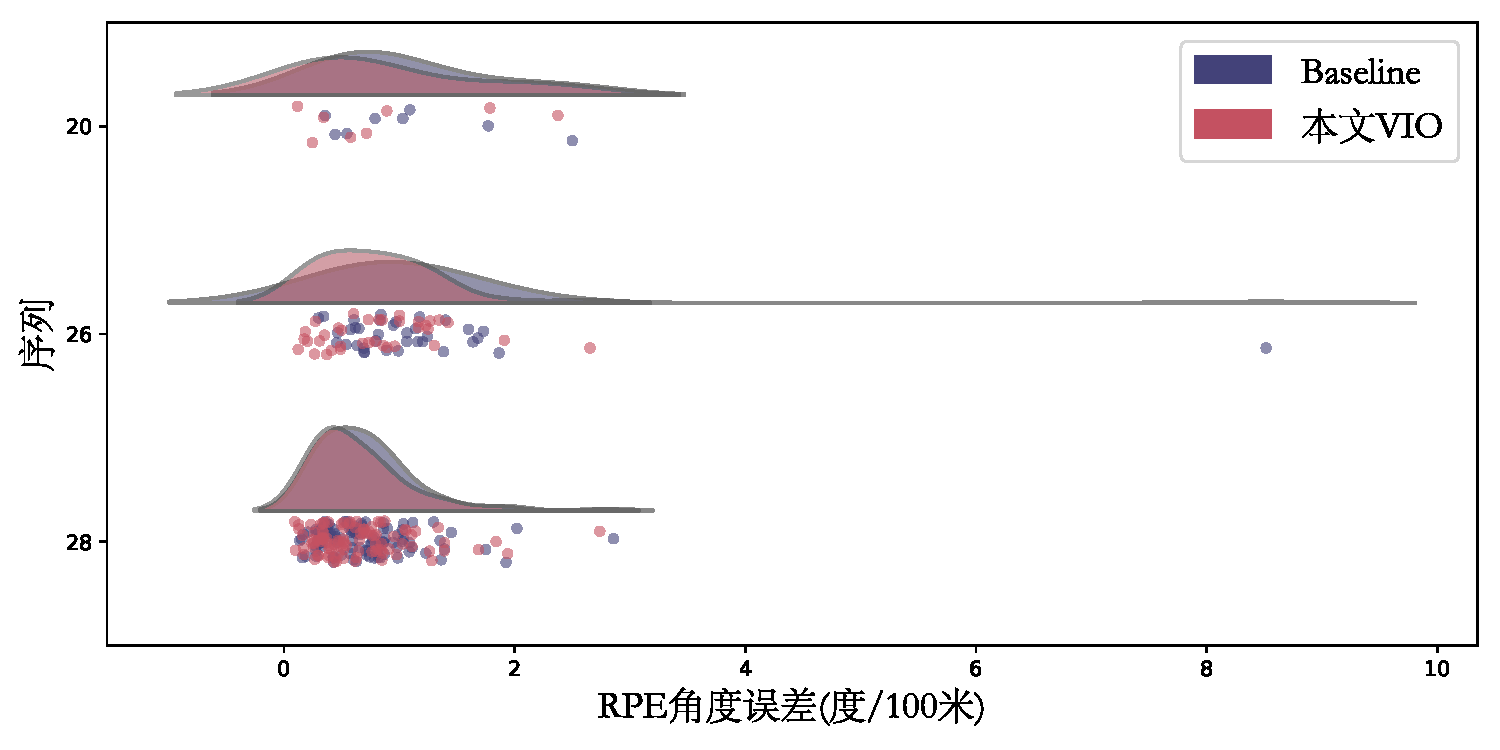
\includegraphics[width=1.0\linewidth]{kaist_cloud.pdf}
  \caption{KAIST数据集上的$RPE_r$\textdownarrow{}分布示意图}
  \label{fig:vio_kaist}
\end{figure}

从表中可以看出,本文设计的PO-VIO在大部分序列上均取得了误差上的改进。对于20-Highway序列,经过改进后,绝对轨迹误差($ATE_t$)从27.55降至26.00,每公里降低约1.55;旋转误差($RPE_r$)也由1.16降低到0.68,减少了约0.48,但相对平移误差($RPE_t$)则略有增加,从19.49上升至20.16。对于26-Dongtan 序列,改进后的$ATE_t$由6.91降至6.45,$RPE_t$从8.91降低到6.54,$RPE_r$也由1.58降低到0.97,三项指标均有明显改善。28-Pangyo序列中,$ATE_t$由5.11降至4.59,$RPE_t$则显著从11.79下降到8.78,而$RPE_r$变化较小,从0.80略降至0.70。

总体来看,尽管20-Highway序列中$RPE_t$有所上升,但本文设计在大部分场景下均能有效降低绝对及相对误差,整体性能得到了提升。

为了展示本文设计的PO-VIO与基线的稳定性效果对比,本文在图~\ref{fig:vio_kaist} 中展示了KAIST数据集上$RPE_r$\textdownarrow{}的分布情况。从图中可以看出,本文PO-VIO在KAIST数据集上的$RPE_r$\textdownarrow{}分布更加集中,且均值更低,相较于基线有着更好的效果。

\subsection{伪观测视觉惯性里程计性能提升的来源分析}
针对PO-VIO性能提升的原因,此处猜测可能是因为本文所提出的伪观测约束项~\eqref{eq:imu_residual} 中仅存在有关旋转和速度的约束,并不直接对平移进行约束,所以在相对平移误差上表现较差,而在相对旋转误差上表现较好。

为了验证这一猜想,本文对车身坐标系的速度量进行分析。分析建立在OF2和OF3两条序列上,这两条序列有着比较突出的特点:OF2序列上本文PO-VIO的$RPE_t$和$RPE_r$(相较于基线VINS-Mono)均有所提升,但是整体幅度较小;OF3序列上本文PO-VIO的$RPE_t$有所下降,但是$RPE_r$有较大提升,而且每100米的旋转误差(相较于基线VINS-Mono)减小了接近1$\degree$/100m。因此选择这两条序列进行分析,能够更好发现本文的速度伪观测约束在何种条件下会对里程计的效果产生积极影响。两条序列上的速度量在车身坐标系的变化如图~\ref{fig:VIO_velocity} 所示。

\begin{figure}
  \centering
  \subcaptionbox*{OF2序列}{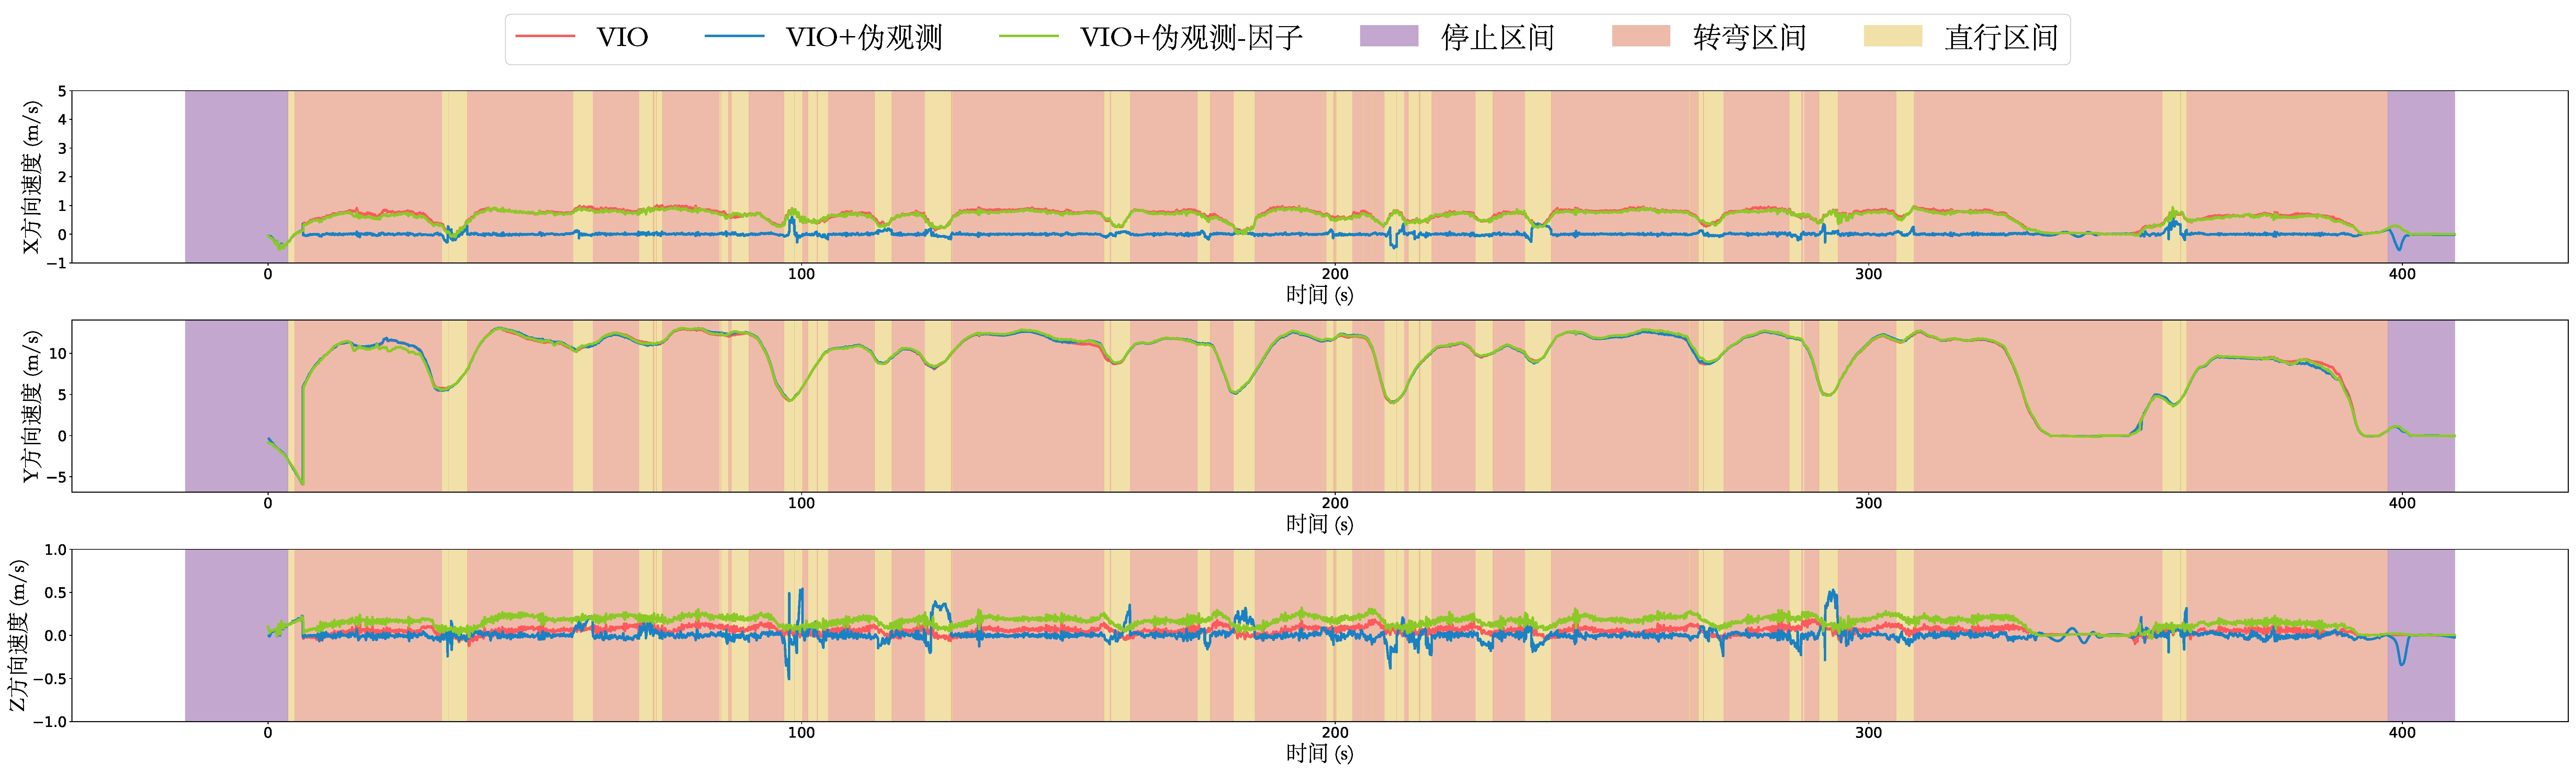
\includegraphics[width=1.0\linewidth]{VIO_velocity_OF2.pdf}}
  \subcaptionbox*{OF3序列}{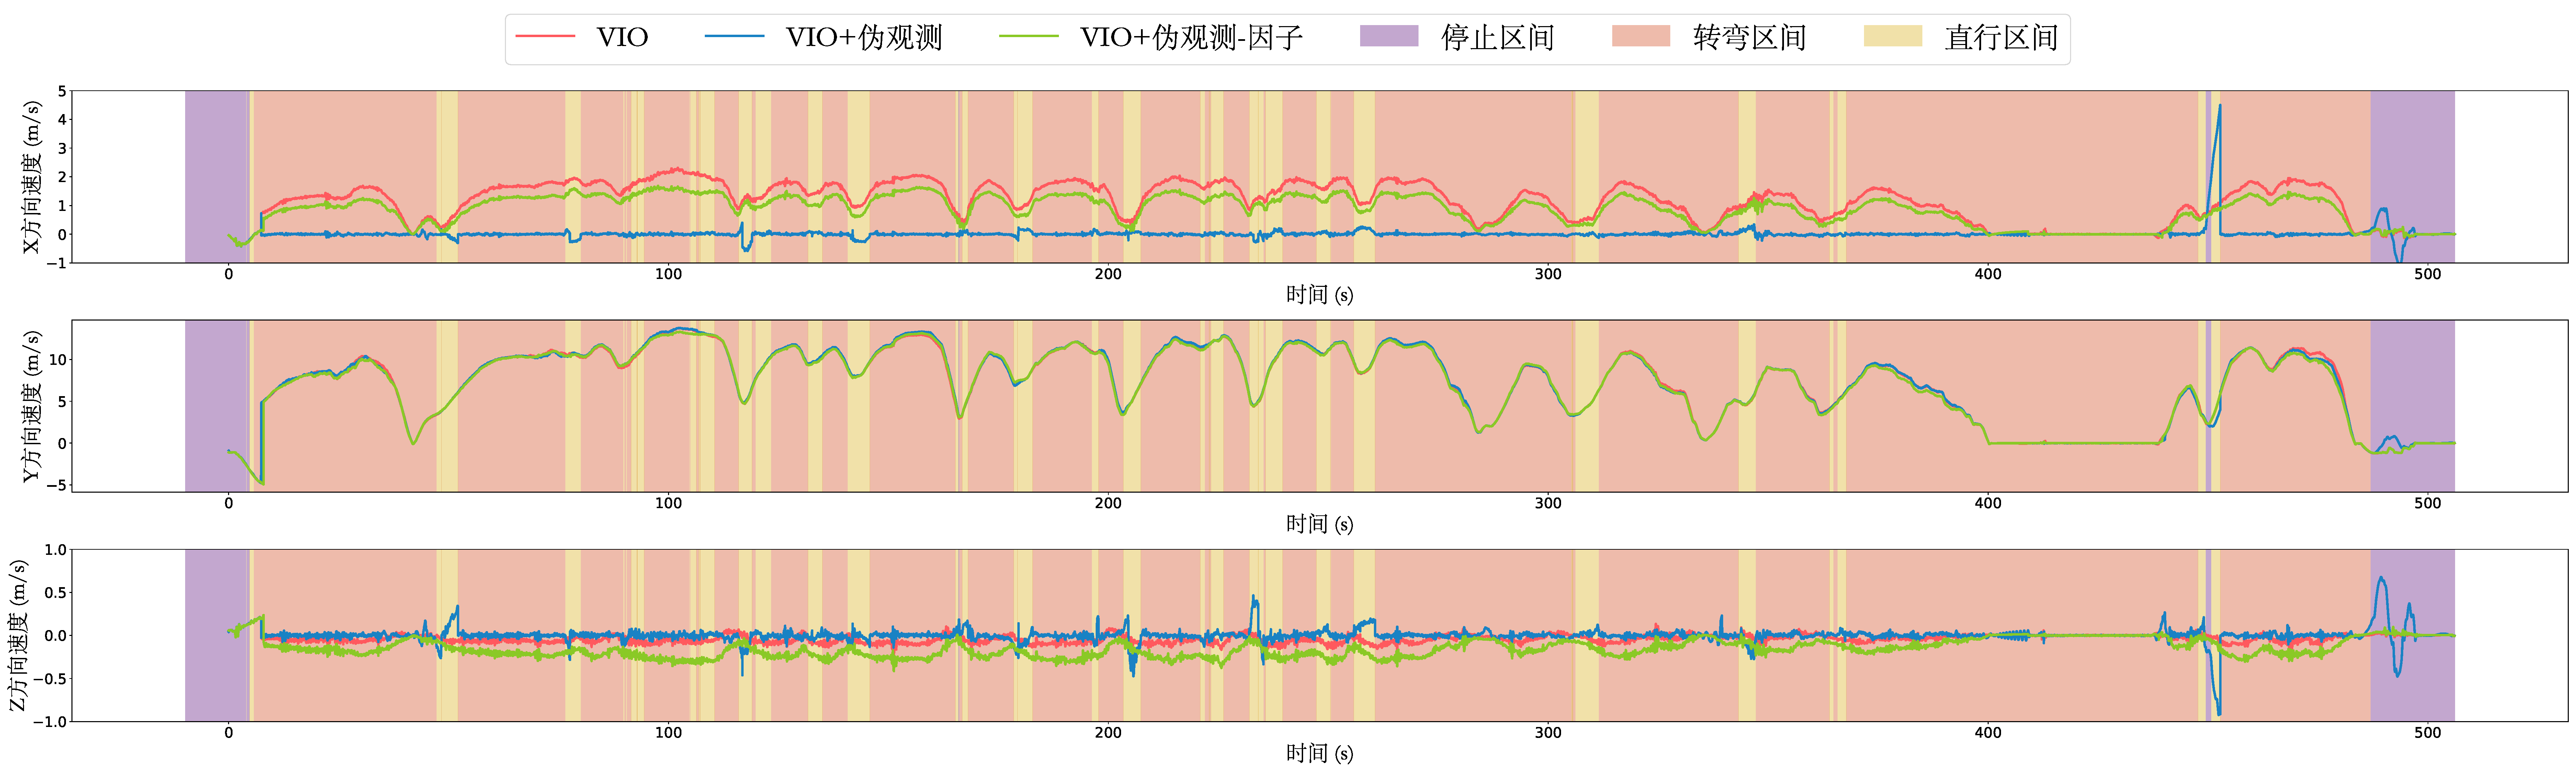
\includegraphics[width=1.0\linewidth]{VIO_velocity_OF3.pdf}}
  \caption{OF2与OF3序列上车身三轴向分速度-时间变化示意图}
  \label{fig:VIO_velocity}
\end{figure}

在每个序列上分别展示了“VIO”、“VIO+伪观测”、“VIO+伪观测-因子”三种情况下的速度变化,其中“VIO”表示使用通用VIO方法获得的速度估计结果;“VIO+伪观测”表示在通用VIO中加入本文所提出的车身状态判断以及伪观测约束后的速度估计结果;“VIO+伪观测-因子”表示在VIO和伪观测约束的基础上,不使用惯性-车体因子进行后端优化。此外,为了将速度变化与车身状态区间直观展示,本文中还将对应车身停止、转弯和直行的区间标注在了速度图中。

从两个序列中的速度变化可以看到:相较于OF2序列,OF3序列的“VIO”在车身横向(X轴方向)和垂直(Z轴方向)速度上有着更大的数值,这说明在OF3序列上基础VIO的速度估计有更大的误差,而在该场景下,经过本文所提出的伪观测约束进行优化后,“VIO+伪观测”横向和垂直速度有了更合理的估计,从而使得OF3上的$RPE_r$有了明显的提升。相较而言,OF2序列上的速度变化较为平缓,所以在该场景下,伪观测约束的加入对于速度估计的影响较小,使得“VIO+伪观测”在OF2序列上的$RPE_r$仅有微弱提升。

此外,观察两个序列下的速度变化,可以发现在OF2上,“VIO+伪观测”的车身横向和垂直速度全过程都有较为平滑的估计结果,相比之下OF3序列上“VIO+伪观测”在最后阶段出现了较明显的起伏,因此其出现了OF3序列上本文方法的$RPE_t$有所下降的现象,而OF2序列上本文方法的$RPE_t$达到同类方法的最优。观察OF3序列的车身三轴向速度变化,还可以看到惯性-车体因子优化对于速度估计的影响:在优化时能够保持较稳定的X轴与Z轴零速度;而不优化则只会有较轻微的抑制作用。这表明了惯性-车体因子联合优化的必要性。


\subsection{消融实验}
为了探究本文提出的VIO方法中各个模块的效果,本节进行了消融实验,消融实验在OF3序列上进行,选择控制的变量包括“VIO”、“惯性-车体因子”、“伪观测约束”、“车身状态判别”和“车身状态真值”,其中“VIO”是基础配置,其他变量的加入均是在VIO的基础上进行的;“惯性-车体因子”表示是否在后端窗口优化时将惯性-车体对齐参数作为优化变量;“伪观测约束”表示是否在后端窗口优化时加入含有伪观测约束的IMU残差;“车身状态判别”表示是否根据车身状态判别神经网络的结果而调整后端优化量;“车身状态真值”表示是否根据车身状态的真值而调整后端优化量,其可以看做是车身状态判别的上限。实验结果如表~\ref{tab:vio_ablation} 所示。表中展示了在不同实验设置下的$ATE_t$、$RPE_t$和$RPE_r$的结果,其中$\checkmark$表示使用了对应的模块。

% \begin{table}
% \centering
% \caption{PO-VIO消融实验}
% \begin{tabular}{cccccccc}
% \toprule
% VIO        & \begin{tabular}[c]{@{}c@{}}惯性-车体\\ 因子\end{tabular} & \begin{tabular}[c]{@{}c@{}}伪观测\\ 约束\end{tabular} & \begin{tabular}[c]{@{}c@{}}车身状态\\ 判别\end{tabular} & \begin{tabular}[c]{@{}c@{}}车身状态\\ 真值\end{tabular} & $ATE_t$\textdownarrow{}       & $RPE_t$\textdownarrow{}     & $RPE_r$\textdownarrow{}      \\ \midrule
% $\checkmark$           &                          &                        &                         &                         & 20.552186            & 5.648737             & 3.411987             \\
% $\checkmark$           & $\checkmark$               & $\checkmark$             &                         &                         & 23.269810            & 5.594315             & 2.588779             \\
% $\checkmark$           & $\checkmark$               & $\checkmark$             & $\checkmark$              &                         & 17.193425            & 5.887755             & 2.543815             \\
% $\checkmark$           & $\checkmark$               & $\checkmark$             &                         & $\checkmark$              & 14.685789            & 5.277349             & 2.522826             \\
% $\checkmark$           &                          & $\checkmark$             &                         & $\checkmark$              & 17.361096            & 5.099256             & 2.577359             \\ \bottomrule
% \end{tabular}
% \label{tab:vio_ablation}
% \end{table}

\begin{table}
\centering
\caption{PO-VIO模块消融实验}
\setlength{\tabcolsep}{3mm}{
\begin{tabular}{cccccccc}
\toprule
VIO        & \begin{tabular}[c]{@{}c@{}}惯性-车体\\ 因子\end{tabular} & \begin{tabular}[c]{@{}c@{}}伪观测\\ 约束\end{tabular} & \begin{tabular}[c]{@{}c@{}}车身状态\\ 判别\end{tabular} & \begin{tabular}[c]{@{}c@{}}车身状态\\ 真值\end{tabular} & $ATE_t$\textdownarrow{}       & $RPE_t$\textdownarrow{}     & $RPE_r$\textdownarrow{}      \\ \midrule
$\checkmark$           &                          &                        &                         &                         & 20.55            & 5.64             & 3.41             \\
$\checkmark$           & $\checkmark$               & $\checkmark$             &                         &                         & 23.26            & 5.59             & 2.58             \\
$\checkmark$           & $\checkmark$               & $\checkmark$             & $\checkmark$              &                         & 17.19            & 5.88             & 2.54             \\
$\checkmark$           & $\checkmark$               & $\checkmark$             &                         & $\checkmark$              & 14.68            & 5.27             & 2.52             \\
$\checkmark$           &                          & $\checkmark$             &                         & $\checkmark$              & 17.36            & 5.09             & 2.57             \\ \bottomrule
\end{tabular}}
\label{tab:vio_ablation}
\end{table}

表中第二行的含义是不论车身处于何种状态,均使用直行时的车身速度假设,因此从前两行的对比中可以发现,当使用了惯性车体因子和伪观测约束后,$ATE_t$产生了明显的上升,但是$RPE_t$有了轻微的下降,$RPE_r$有了明显的下降。这说明了惯性车体因子和伪观测约束的加入对于车身旋转的估计有着重要的影响,但是这会对平移的估计产生一定负面影响。即说明如果全程使用直行时的车身速度假设,会对里程计的平移估计精度产生负面影响,但对旋转的估计精度有积极影响。

表中第三行在第二行的基础上加入了对车身状态的预测,虽然预测与真实情况可能存在偏差,但是可以从数据上得出:当加入了车身状态判别后,$ATE_t$产生明显的下降,$RPE_t$有所增加,$RPE_r$有轻微下降,这说明了车身状态判别对于绝对定位精度的提升有着重要的影响。虽然其本身存在的状态预测误差则会对相对位移的估计产生一定的负面影响,但是综合来看其对于绝对位置和旋转角度估计的精度提升可以使其忽略对相对位移估计产生的负面影响。

表中第四行在第三行的基础上将车身状态的预测值替换为真值,这一行为对$ATE_t$、$RPE_t$和$RPE_r$三个指标都产生了增益效果,这侧面证明了:当使用预测值时产生的相对位移估计精度损失是由于预测值的误差导致的,而当使用真值时,这一误差被消除,所以在$ATE_t$、$RPE_t$和$RPE_r$三个指标上都取得了较大的进步。

表中最后一行在第四行的基础上去掉了惯性车体因子,即在优化过程中不优化惯性-车体因子,而仅使用初始量。这一行相较于第四行的结果是:$ATE_t$和$RPE_r$产生了一定程度的损失,但是$RPE_t$却达到了最好效果。这一行的结果表明:惯性-车体因子的实时优化对于绝对位置精度和旋转估计有着重要的积极影响,但是对于相对平移估计则有着负面影响。但是综合来看,优化惯性-车体因子对于绝对位置和相对旋转的估计的提升明显,而对于相对位置估计精度的影响有限,因此有保留的必要。

\section{地图定位模块与系统整体测试}
地图定位模块的测试在KITTI数据集和4Seasons数据集上进行,本节将分别对两个数据集上的测试结果进行展示;此外还对模块的各个部分进行了消融实验和效率分析。需要注意的是,由于地图定位模块是系统的最关键部分,其输出等同于系统的最终输出,因此其测试结果也可代表系统整体表现。

\subsection{系统精度测试}
\subsubsection{KITTI数据集测试}

在KITTI数据集上,本文的地图定位模块测试结果如图~\ref{fig:loc_kitti} 、图~\ref{fig:loc_kitti_cdf} 和表~\ref{tab:loc_kitti} 所示,在表~\ref{tab:loc_kitti} 中以加粗字体和红底标出最佳表现。

\begin{figure}
  \centering
  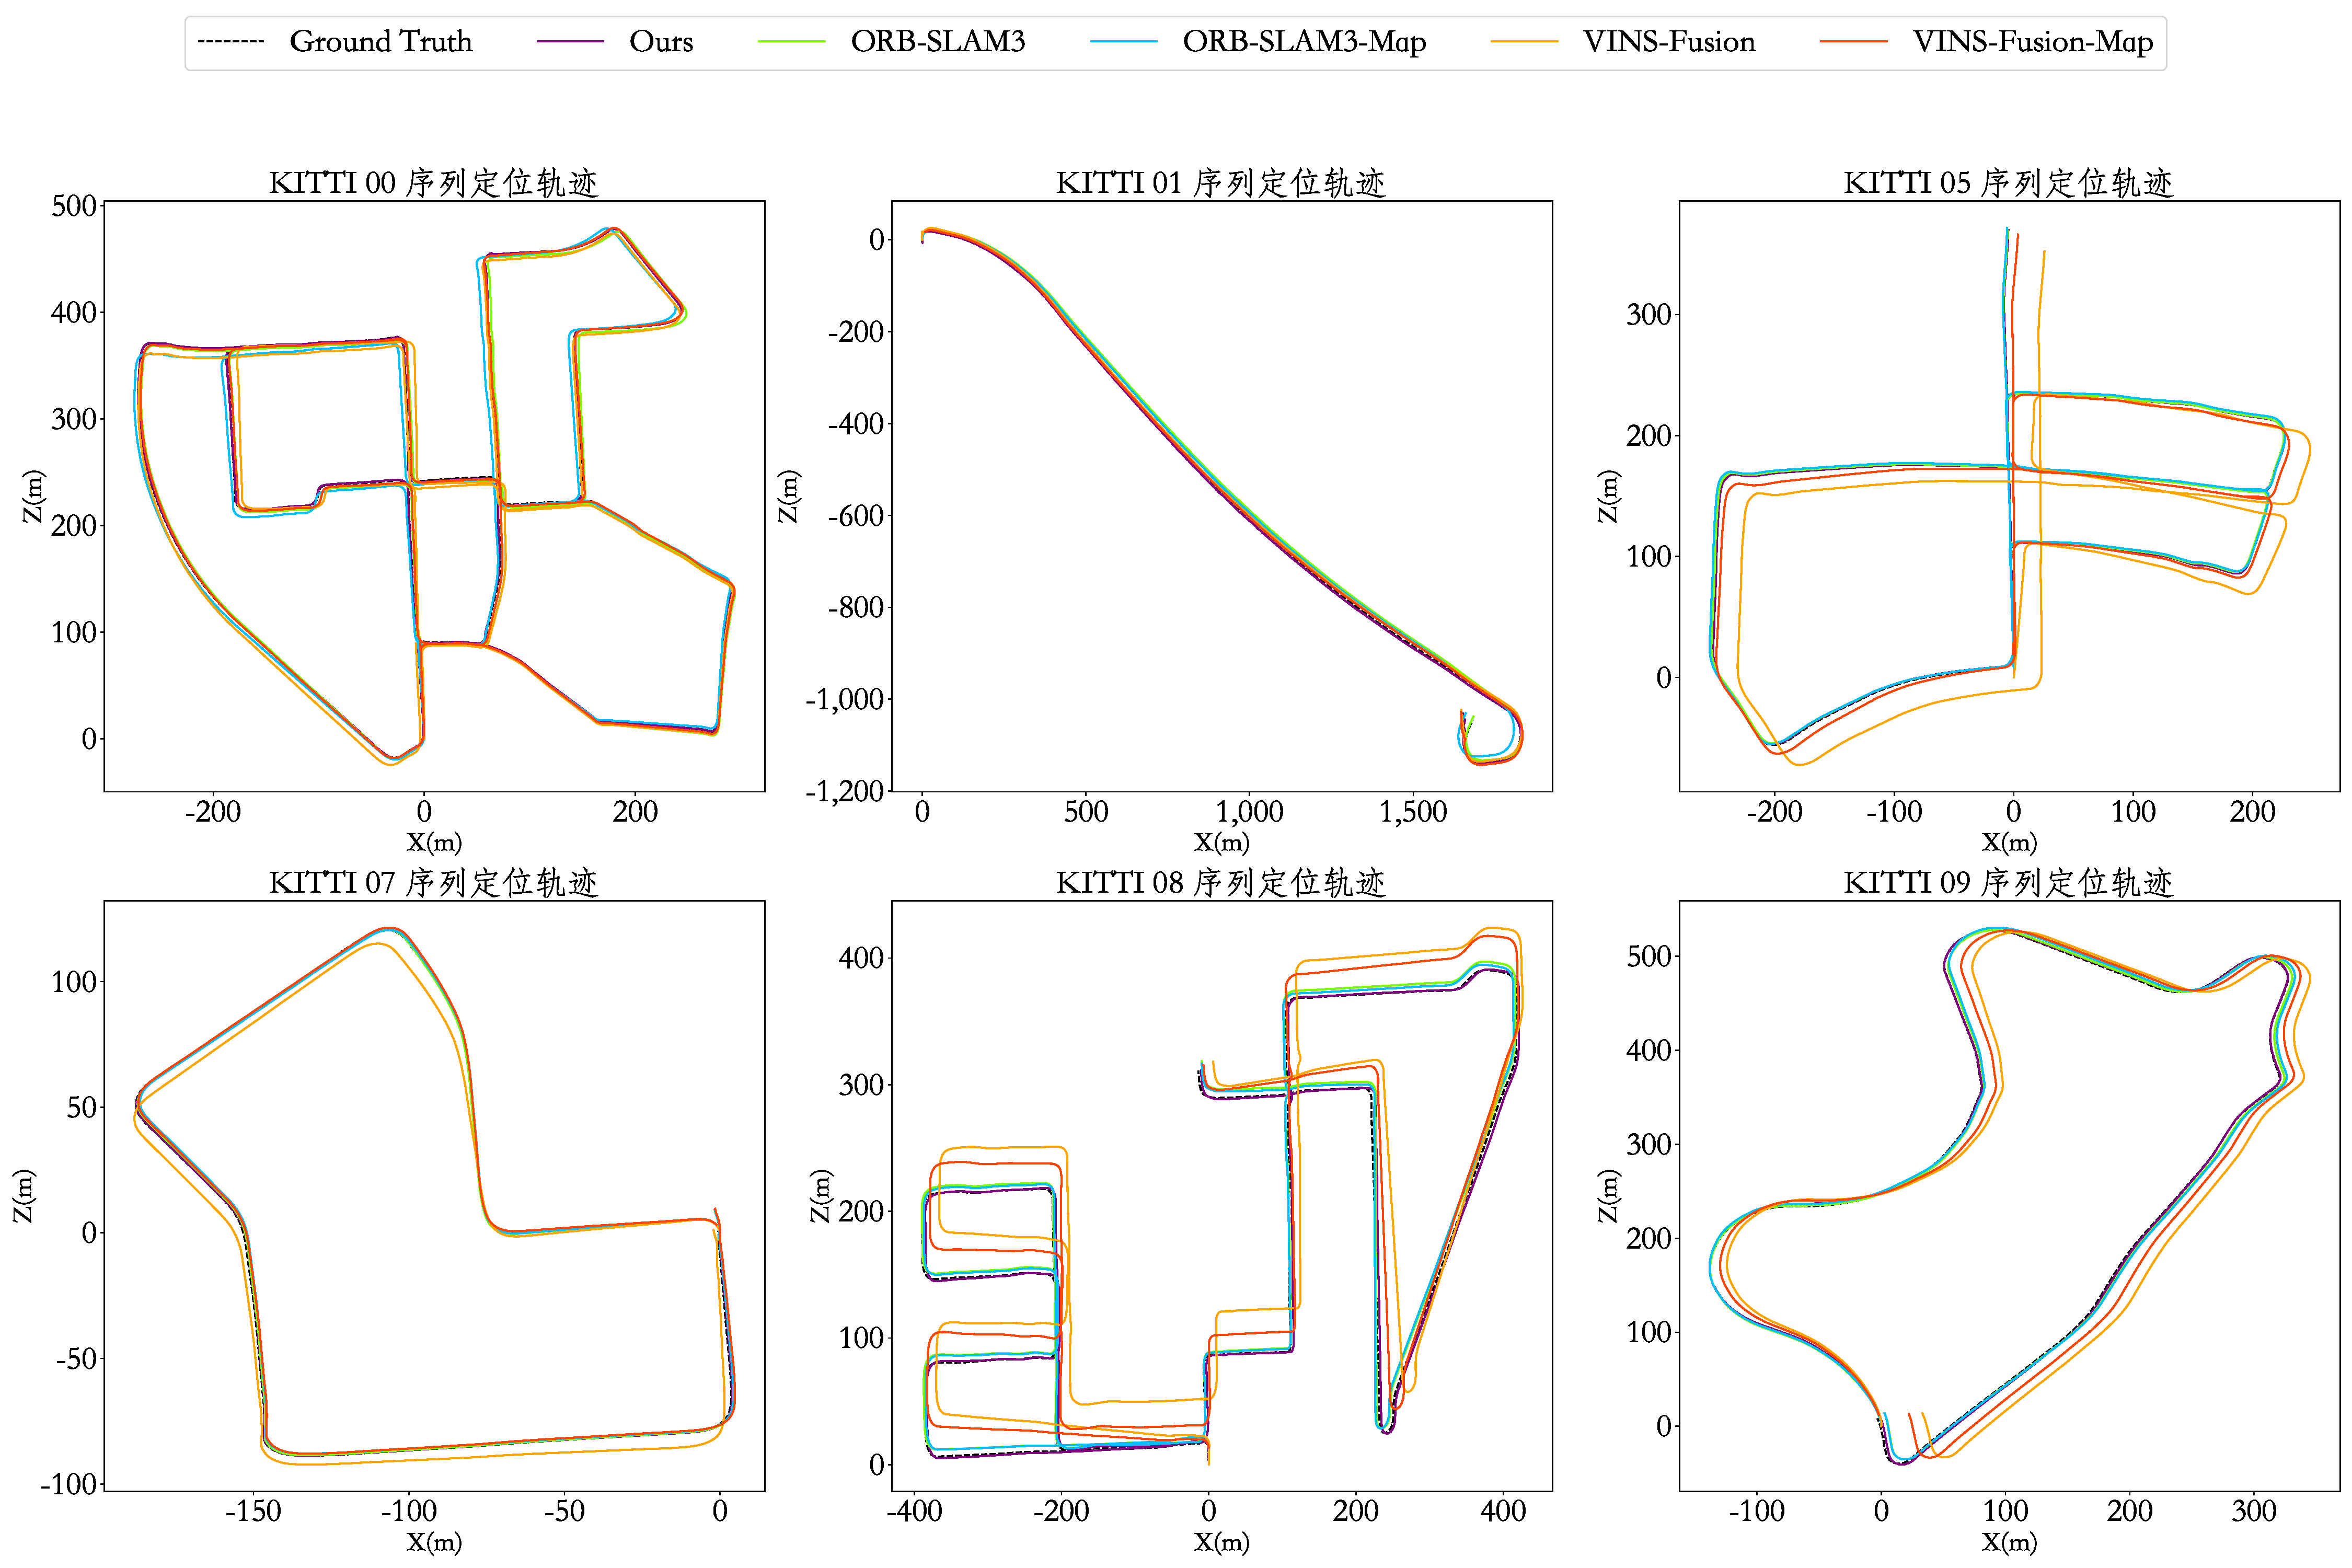
\includegraphics[width=0.9\linewidth]{loc_kitti.pdf}
  \caption{多种定位方法在KITTI数据集上的定位轨迹}
  \label{fig:loc_kitti}
\end{figure}

对比的方法包括VINS-Fusion(VINS)、VINS-Fusion-Map(VINSM)、ORB-SLAM3(ORB)和ORB-SLAM3-Map(ORBM)进行对比,其中VINS-Fusion-Map和ORB-SLAM3-Map是VINS-Fusion和ORB-SLAM3的地图版本。

如图~\ref{fig:loc_kitti}所示,本文的方法在图中展示的六个序列中均成功实现了精确的定位轨迹。然而,由于ORB-SLAM3、本文提出的方法与真实轨迹之间几乎完全重合,导致性能对比变得具有挑战性。因此,在图~\ref{fig:loc_kitti_cdf}中进一步展示了累计分布函数(Cumulative Distribution Function, CDF)。除序列05外,在所有序列中,本文的方法在较低的平移误差下迅速达到近乎完整的准确率(CDF接近1),显著优于其他方法,而其他方法则表现出更大的误差。对于序列05,本文的方法在较低的平移误差下也表现出更高的累计概率,进一步证明了其卓越的定位精度。综上所述,CDF曲线所展现出的明显性能差距验证了本文提出方法在精度、鲁棒性和可靠性方面的优势,使其非常适合于高精度、可靠性的视觉定位任务。

从表~\ref{tab:loc_kitti} 中KITTI数据集上多项指标的对比结果来看,不同方法在不同序列上表现存在较大差异。对于绝对轨迹误差$ATE_t$指标,本文方法在序列 00、01、02、05、06、07、08 和 10 上均取得了最低值,说明在绝对位姿精度上具有较明显的优势;仅在序列 04 上,ORB-SLAM3表现更优,而序列 09 的结果略有争议,尽管 VINS 在此处显示出稍低的误差,但总体来看,本文方法在大部分序列中均展现出更好的平稳性。

\begin{figure}
  \centering
  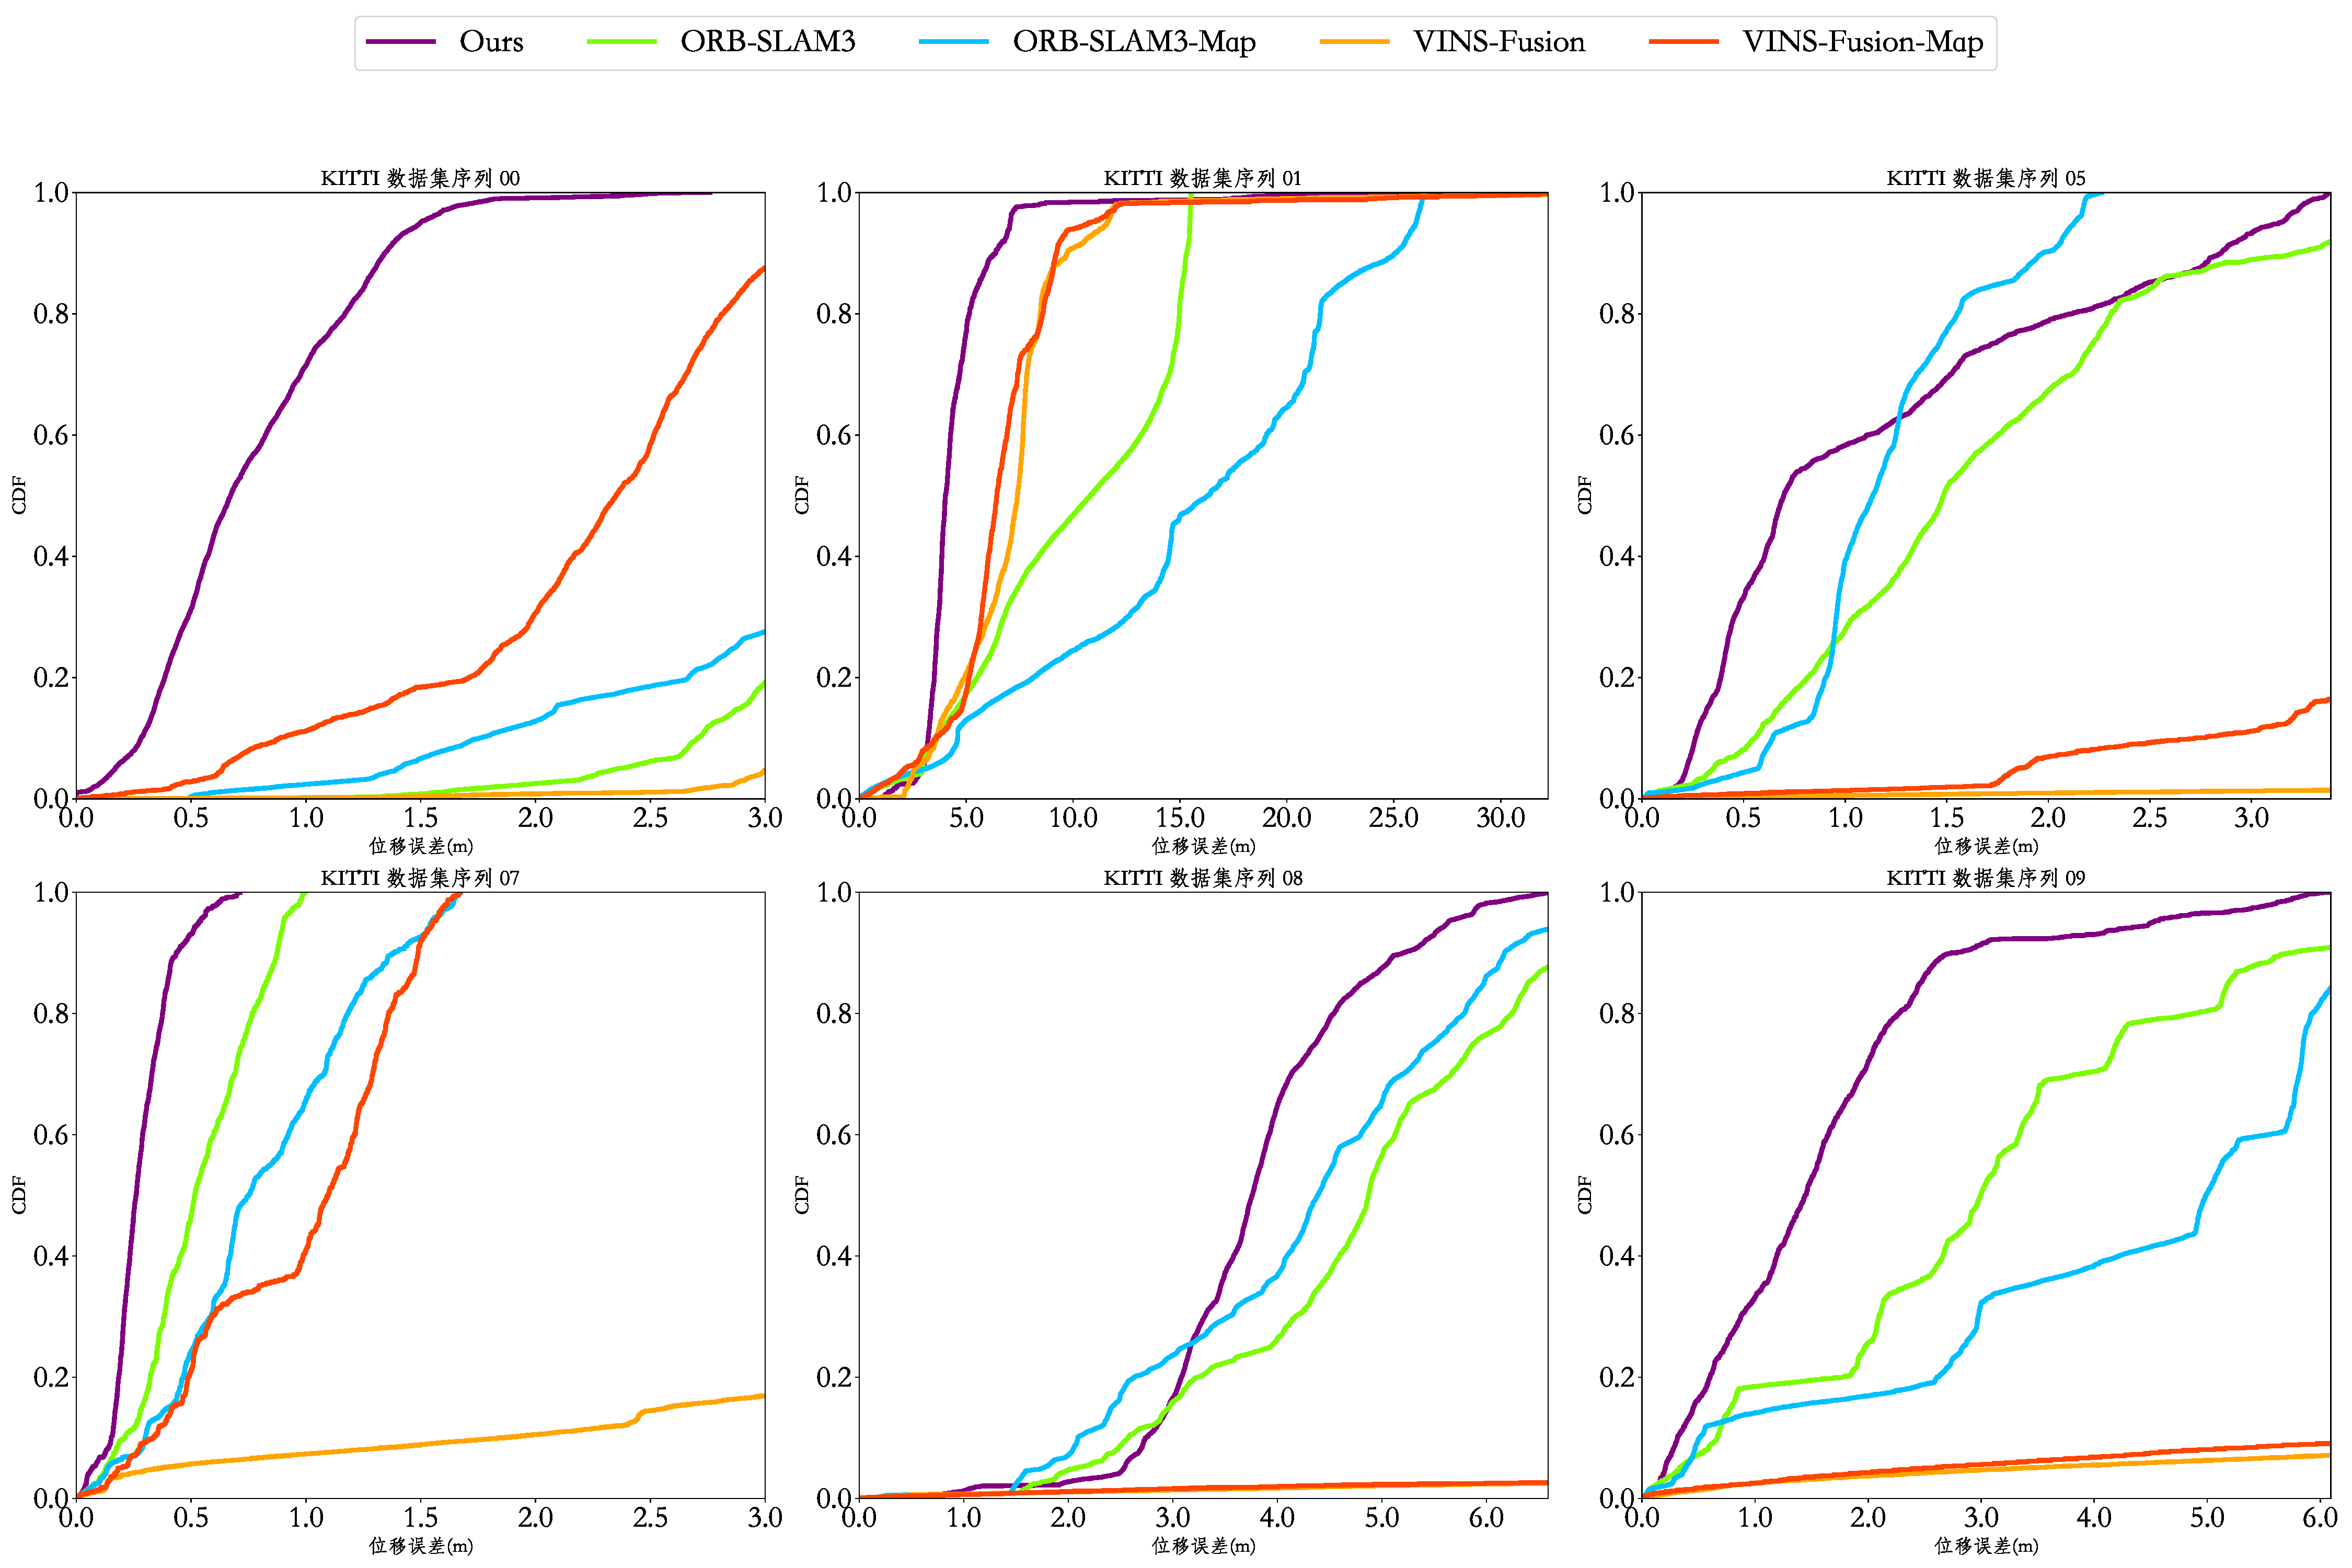
\includegraphics[width=0.9\linewidth]{loc_kitti_cdf.pdf}
  \caption{多种定位方法在KITTI数据集上的位移误差CDF曲线}
  \label{fig:loc_kitti_cdf}
\end{figure}

对于相对平移误差$RPE_t$而言,各方法的表现相对分散。本文方法在序列 01、02、07 和 08 上表现突出,但在其他序列中,ORB-SLAM3、ORB-SLAM3-Map或其他方法有时能获得更低的误差,表明在平移精度方面,各算法对场景和运动状态的敏感性不同。而在相对旋转误差$RPE_r$方面,本文方法在部分序列,如 00、07、08、09,中取得了较低的值,体现出在角度估计上的一定优势,但在序列 01、02 和 04 上,ORB-SLAM3 或 ORB-SLAM3-Map 的表现更佳,说明在旋转精度上,算法之间仍存在细微差距。

\begin{table}
\centering
\begin{threeparttable}
\caption{多种定位方法在KITTI数据集上的多指标对比}
\begin{tabular}{lccccccccccc}
\toprule
方法    & 指标                    & 00            & 01            & 02            & 04            & 05            & 06            & 07            & 08            & 09            & 10            \\ \midrule
ORB   & \multirow{5}{*}{$ATE_t$\textdownarrow{}}  & 3.51          & 4.92          & 5.70          & \cellcolor[HTML]{FFCCC9}\textbf{0.27} & 1.84          & 1.68          & 0.96          & 3.32          & 3.37          & 0.90          \\
ORBM  &                       & 7.19          & 10.11         & 10.32         & 0.98          & 1.54          & 2.35          & 1.67          & 5.36          & 7.61          & 0.95          \\
VINS  &                       & 5.95          & 6.49          & 5.99          & 1.08          & 5.98          & 3.48          & 2.41          & 3.85          & \cellcolor[HTML]{FFCCC9}\textbf{1.78}          & 3.78          \\
VINSM &                       & 3.92          & 8.01          & 13.08         & 1.23          & 3.88          & 1.79          & 0.65          & 9.89          & 6.17          & 3.63          \\
本文方法    &                       & \cellcolor[HTML]{FFCCC9}\textbf{0.97} & \cellcolor[HTML]{FFCCC9}\textbf{4.09} & \cellcolor[HTML]{FFCCC9}\textbf{0.70} & 0.53          & \cellcolor[HTML]{FFCCC9}\textbf{1.24} & \cellcolor[HTML]{FFCCC9}\textbf{1.56} & \cellcolor[HTML]{FFCCC9}\textbf{0.21} & \cellcolor[HTML]{FFCCC9}\textbf{1.68} & 1.87 & \cellcolor[HTML]{FFCCC9}\textbf{0.82} \\ \midrule
ORB   & \multirow{5}{*}{$RPE_t$\textdownarrow{}} & 0.88          & 1.44          & 0.77          & \cellcolor[HTML]{FFCCC9}\textbf{0.46} & 0.62          & 0.89          & 0.89          & 1.03          & \cellcolor[HTML]{FFCCC9}\textbf{0.86} & 0.62          \\
ORBM  &                       & 0.69          & 1.46          & 0.77          & 0.49          & \cellcolor[HTML]{FFCCC9}\textbf{0.40} & \cellcolor[HTML]{FFCCC9}\textbf{0.46} & 0.52          & 1.04          & 0.87          & \cellcolor[HTML]{FFCCC9}\textbf{0.61} \\
VINS  &                       & 3.45          & 12.18         & 2.65          & 2.71          & 1.41          & 1.33          & 1.17          & 3.46          & 4.45          & 2.38          \\
VINSM &                       & 1.23          & 2.44          & 1.49          & 1.37          & 1.46          & 0.88          & 0.71          & 1.66          & 1.97          & 2.45          \\
本文方法    &                       & \cellcolor[HTML]{FFCCC9}\textbf{0.74} & \cellcolor[HTML]{FFCCC9}\textbf{1.44} & \cellcolor[HTML]{FFCCC9}\textbf{0.68} & 1.87          & 0.75          & 0.84          & \cellcolor[HTML]{FFCCC9}\textbf{0.39} & \cellcolor[HTML]{FFCCC9}\textbf{0.96} & 1.03          & 0.82          \\ \midrule
ORB   & \multirow{5}{*}{$RPE_r$\textdownarrow{}} & 0.31          & \cellcolor[HTML]{FFCCC9}\textbf{0.19} & \cellcolor[HTML]{FFCCC9}\textbf{0.28} & 0.19          & 0.26          & 0.27          & 0.50          & 0.31          & 0.25          & 0.29          \\
ORBM  &                       & 0.26          & \cellcolor[HTML]{FFCCC9}\textbf{0.19} & \cellcolor[HTML]{FFCCC9}\textbf{0.28} & \cellcolor[HTML]{FFCCC9}\textbf{0.08} & \cellcolor[HTML]{FFCCC9}\textbf{0.16} & \cellcolor[HTML]{FFCCC9}\textbf{0.15} & 0.30          & 0.31          & 0.25          & \cellcolor[HTML]{FFCCC9}\textbf{0.28} \\
VINS  &                       & 1.45          & 3.54          & 1.26          & 0.62          & 0.69          & 0.72          & 0.87          & 1.77          & 1.87          & 0.94          \\
VINSM &                       & 0.73          & 0.48          & 0.56          & 0.69          & 0.67          & 0.58          & 0.57          & 0.65          & 0.59          & 0.99          \\
本文方法    &                       & \cellcolor[HTML]{FFCCC9}\textbf{0.27} & 0.34          & 0.30          & 0.30          & 0.19          & 0.17          & \cellcolor[HTML]{FFCCC9}\textbf{0.26} & \cellcolor[HTML]{FFCCC9}\textbf{0.29} & \cellcolor[HTML]{FFCCC9}\textbf{0.19} & 0.30          \\ \bottomrule
\end{tabular}
\label{tab:loc_kitti}
\begin{tablenotes}
  \item [a] ORB和ORBM分别表示ORB-SLAM3和ORB-SLAM3-Map。
  \item [b] VINS和VINSM分别表示VINS-Fusion和VINS-Fusion-Map。
\end{tablenotes}
\end{threeparttable}
\end{table}


\subsubsection{综合(Office Loop)场景测试}
4Seasons数据集实在同一条线路上多次采集获得的,采集的时间跨度从几十分钟到一年,所以其场景相对于KITTI数据集有更多的变化,包括季节、天气、晨昏等。本文首先在Office Loop的一般性场景下进行测试。一般性场景测时的建图序列为2020.03.24 17:36拍摄,而定位序列为2020.03.24 17:45拍摄,两个场景差异较小,因此可以同时比较多个方法的表现。

% \begin{table}
% \centering
% \begin{threeparttable}[c]
% \caption{4Seasons数据集Office Loop场景第2序列指标对比}
% \begin{tabular}{lccccccc}
% \toprule
% 方法                                     & 时间                                                                         & 季节                   & 天气                   & 晨昏                   & $ATE_t$\textdownarrow{}               & $RPE_t$\textdownarrow{}              & $RPE_r$\textdownarrow{}              \\ \midrule
% 离线建图                                   & \begin{tabular}[c]{@{}c@{}}03.24\\ 17:36 \\ (OF1)\end{tabular}                   & 春季                   & 晴朗                   & 下午                   & 0.814881          & 0.929358          & 1.014480          \\ \midrule
% VINS-Mono                              & \multirow{10}{*}{\begin{tabular}[c]{@{}c@{}}03.24\\ 17:45 \\ (OF2)\end{tabular}} & \multirow{10}{*}{春季} & \multirow{10}{*}{晴朗} & \multirow{10}{*}{下午} & 7.878626          & 2.330876          & 0.783557          \\
% VINS-Mono w/ Map1                      &                                                                            &                      &                      &                      & 3.092430          & N/A               & N/A               \\
% VINS-Monow/ Map2                       &                                                                            &                      &                      &                      & 2.440850          & N/A               & N/A               \\
% ORB-SLAM3                              &                                                                            &                      &                      &                      & 15.621815         & 3.222846          & 0.890233          \\
% ORB-SLAM3 w/ Map3                      &                                                                            &                      &                      &                      & 19.249121         & N/A               & N/A               \\
% VINS-Fusion w/  RTK &                                                                            &                      &                      &                      & 1.801669          & 1.500405          & 1.085638          \\
% VLS                                    &                                                                            &                      &                      &                      & 1.715343          & 1.630718          & \cellcolor[HTML]{FFCCC9}\textbf{0.668220} \\
% GPLD                                   &                                                                            &                      &                      &                      & 8.720000          & N/A               & N/A               \\
% MVIL                                   &                                                                            &                      &                      &                      & 6.450000          & N/A               & N/A               \\
% 本文方法                                   &                                                                            &                      &                      &                      & \cellcolor[HTML]{FFCCC9}\textbf{0.777091} & \cellcolor[HTML]{FFCCC9}\textbf{1.124076} & 0.759267          \\ \bottomrule
% \end{tabular}
% \label{tab:loc_4seasons_of2}
% \begin{tablenotes}
%   \item [a] Map1表示使用VINS-Mono建图结果
%   \item [b] Map2表示使用本文离线建图结果
%   \item [c] Map3表示使用ORB-SLAM3建图结果
%   \item [d] RTK表示使用了RTK-GPS数据,其定位精度达到厘米级
% \end{tablenotes}
% \end{threeparttable}
% \end{table}

% 测试结果如表~\ref{tab:loc_4seasons_of2} 所示,其中包括了VINS-Mono、VINS-Fusion w/ RTK、ORB-SLAM3、VLS\cite{yang2022real}(2022)、GPLD\cite{hao2023global}(2023)、MVIL\cite{zhang2023map}(2023)等方法与本文方法的对比,其中VINS-Fusion w/ RTK使用了高精度(厘米级)GNSS信号,而VLS、GPLD、MVIL则是近期涌现的三种基于地图的定位方法。

% 首先在OF1和OF2两个序列上进行实验,这两个序列由于拍摄时间接近,所以场景变化不大,因此在其中进行的实验还包括了VINS-Mono w/ Map1、VINS-Mono w/ Map2、ORB-SLAM3 w/ Map3等方法的对比。从表~\ref{tab:loc_4seasons_of2} 中可以看出,本文方法在$ATE_t$和$RPE_t$上均取得了最佳表现,而在$RPE_r$上略逊于VLS方法,此外本文方法是第一个将定位精度提升到1米以内的方法,本文将其在卫星图上的定位结果展示如图~\ref{fig:loc_4seasons_of2} 所示。

% \begin{figure}
%   \centering
%   \subcaptionbox{OF1序列建图轨迹\label{fig:loc_4seasons_of1}}{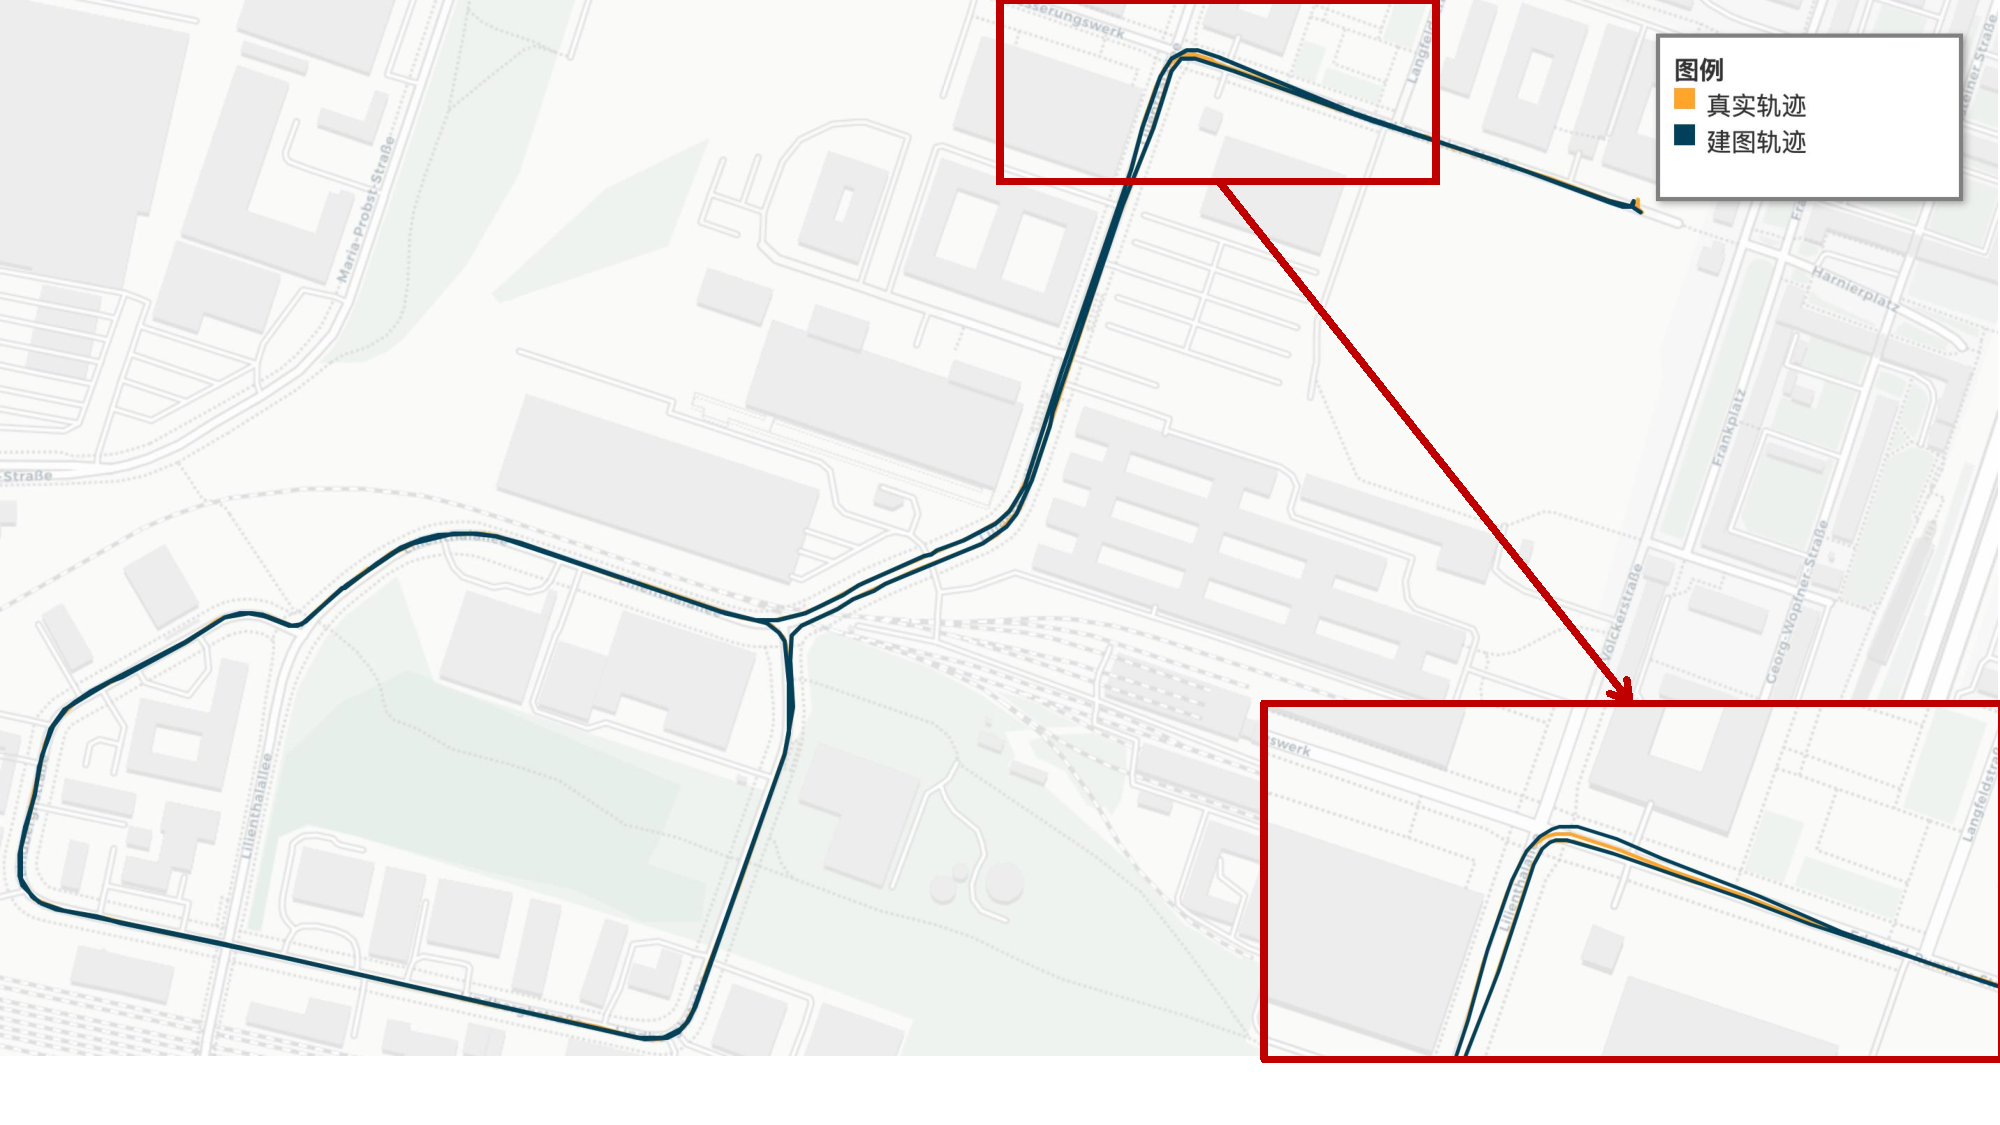
\includegraphics[width=0.47\linewidth]{OF1_zoomin.pdf}}
%   \subcaptionbox{OF2序列定位轨迹\label{fig:loc_4seasons_of2}}{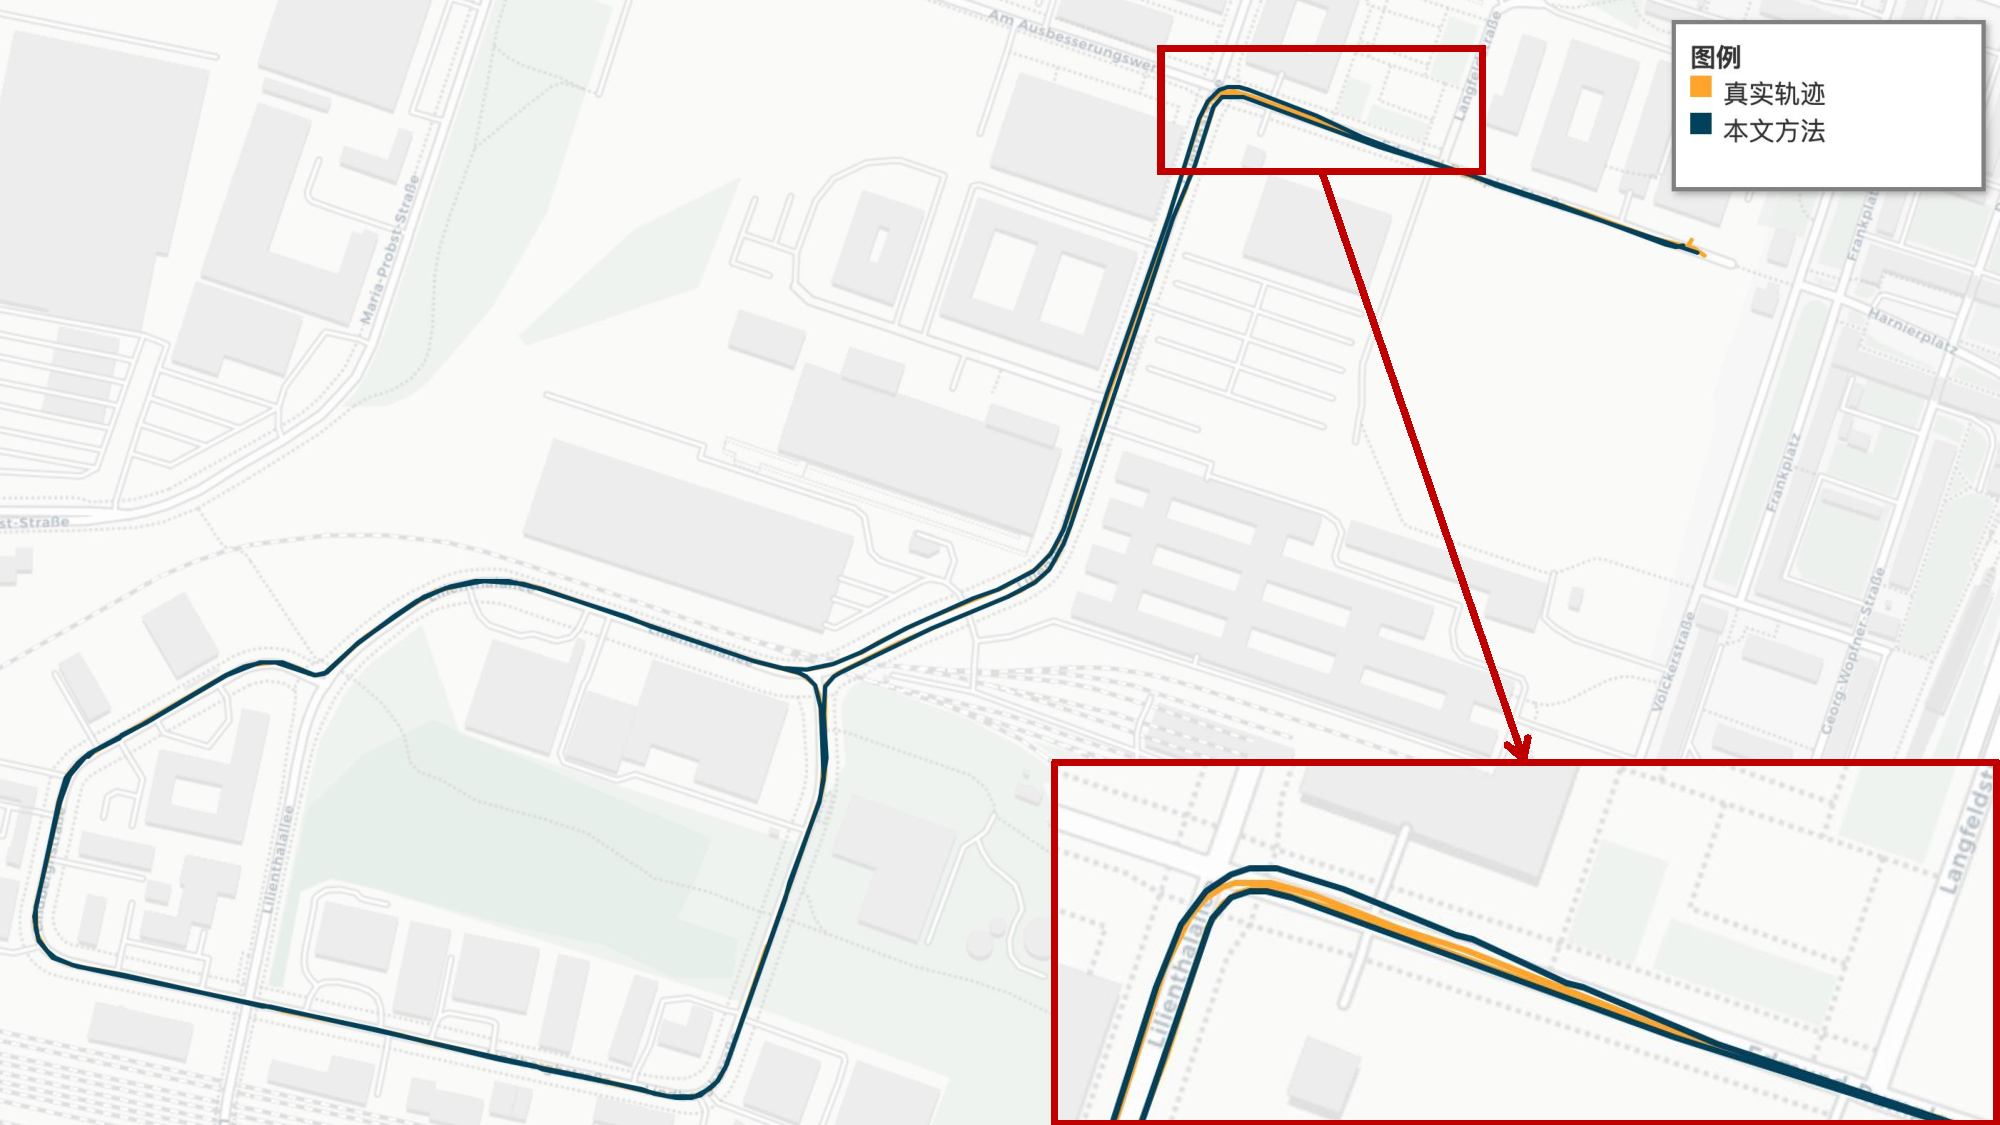
\includegraphics[width=0.45\linewidth]{OF2_zoomin.pdf}}
%   \caption{4Seasons数据集定位结果及误差分析}
%   \label{fig:loc_gnssmap}
% \end{figure}


测试结果如表~\ref{tab:loc_4seasons_of2} 所示,其中包括了VINS-Mono、VINS-Fusion w/ RTK、ORB-SLAM3、VLS\cite{yang2022real}(2022)、GPLD\cite{hao2023global}(2023)、MVIL\cite{zhang2023map}(2023)等方法与本文方法的对比,其中VINS-Fusion w/ RTK使用了高精度(厘米级)GNSS信号,而VLS、GPLD、MVIL则是近期涌现的三种基于地图的定位方法。

\begin{table}
\centering
\begin{threeparttable}[c]
\caption{多种定位方法在OF2序列上的多指标对比}
\setlength{\tabcolsep}{2.65mm}{
\begin{tabular}{lccccccc}
\toprule
方法                                     & 时间                                                                         & 季节                   & 天气                   & 晨昏                   & $ATE_t$\textdownarrow{}               & $RPE_t$\textdownarrow{}              & $RPE_r$\textdownarrow{}              \\ \midrule
离线建图                                   & \begin{tabular}[c]{@{}c@{}}03.24\\ 17:36 \\ (OF1)\end{tabular}                   & 春季                   & 晴朗                   & 下午                   & 0.81          & 0.92          & 1.01          \\ \midrule
VINS-Mono                              & \multirow{10}{*}{\begin{tabular}[c]{@{}c@{}}03.24\\ 17:45 \\ (OF2)\end{tabular}} & \multirow{10}{*}{春季} & \multirow{10}{*}{晴朗} & \multirow{10}{*}{下午} & 7.87          & 2.33          & 0.78          \\
VINS-Mono w/ Map1                      &                                                                            &                      &                      &                      & 3.09          & N/A               & N/A               \\
VINS-Monow/ Map2                       &                                                                            &                      &                      &                      & 2.44          & N/A               & N/A               \\
ORB-SLAM3                              &                                                                            &                      &                      &                      & 15.62         & 3.22          & 0.89          \\
ORB-SLAM3 w/ Map3                      &                                                                            &                      &                      &                      & 19.24         & N/A               & N/A               \\
VINS-Fusion w/  RTK &                                                                            &                      &                      &                      & 1.80          & 1.50          & 1.08          \\
VLS                                    &                                                                            &                      &                      &                      & 1.71          & 1.63          & \cellcolor[HTML]{FFCCC9}\textbf{0.66} \\
GPLD                                   &                                                                            &                      &                      &                      & 8.72          & N/A               & N/A               \\
MVIL                                   &                                                                            &                      &                      &                      & 6.45          & N/A               & N/A               \\
本文方法                                   &                                                                            &                      &                      &                      & \cellcolor[HTML]{FFCCC9}\textbf{0.77} & \cellcolor[HTML]{FFCCC9}\textbf{1.12} & 0.75          \\ \bottomrule
\end{tabular}}
\label{tab:loc_4seasons_of2}
\begin{tablenotes}
  \item [a] Map1表示使用VINS-Mono建图结果。
  \item [b] Map2表示使用本文离线建图结果。
  \item [c] Map3表示使用ORB-SLAM3建图结果。
  \item [d] RTK表示使用了RTK-GNSS数据,其定位精度达到厘米级。
\end{tablenotes}
\end{threeparttable}
\end{table}

首先在OF1和OF2两个序列上进行实验,这两个序列由于拍摄时间接近,所以场景变化不大,因此在其中进行的实验还包括了VINS-Mono w/ Map1、VINS-Mono w/ Map2、ORB-SLAM3 w/ Map3等方法的对比。从表~\ref{tab:loc_4seasons_of2} 中可以看出,本文方法在$ATE_t$和$RPE_t$上均取得了最佳表现,而在$RPE_r$上略逊于VLS方法,此外本文方法是第一个将定位精度提升到1米以内的方法,本文将其在卫星图上的定位结果展示如图~\ref{fig:loc_gnssmap} 的子图~\ref{fig:loc_4seasons_of2} 所示。

\begin{figure}
  \centering
  \subcaptionbox{OF1序列建图轨迹\label{fig:loc_4seasons_of1}}{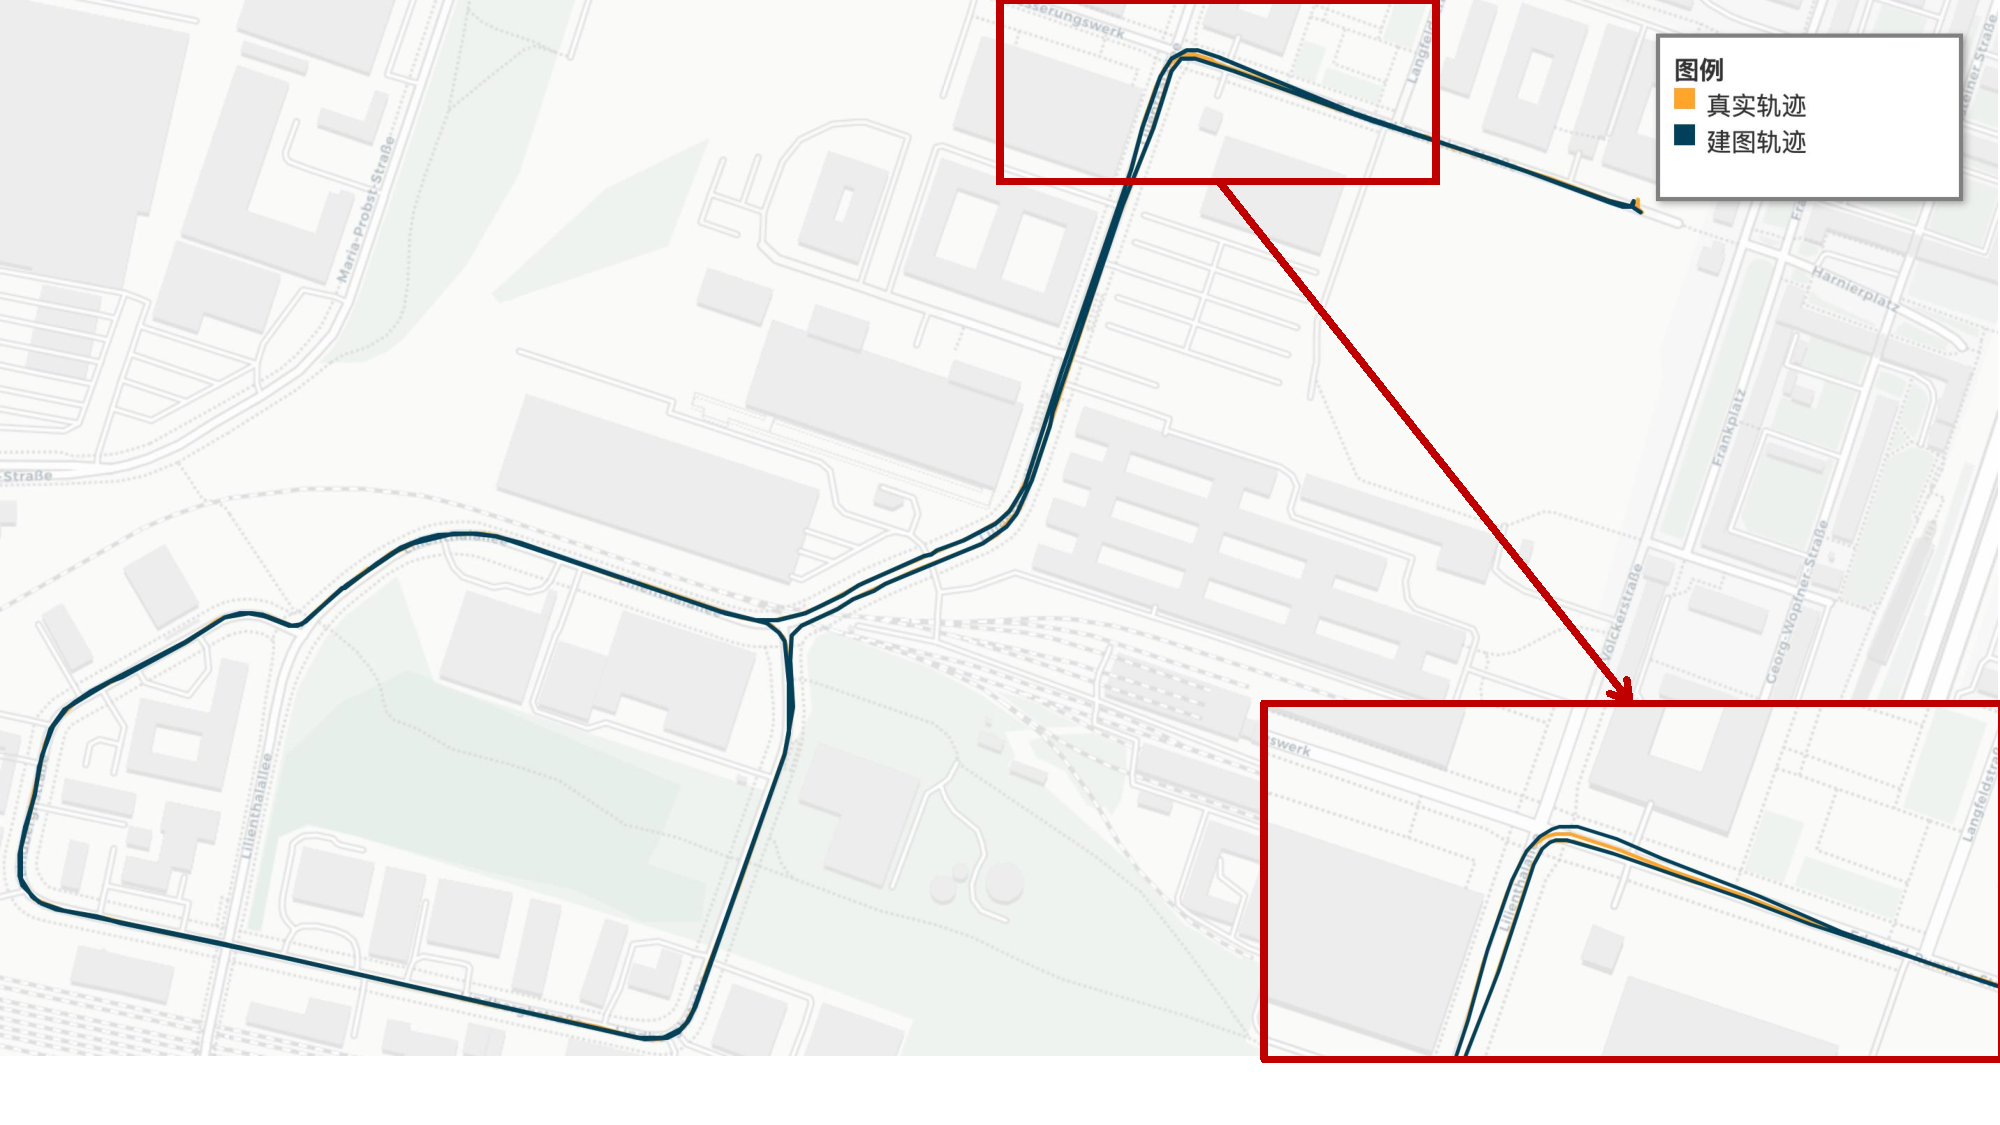
\includegraphics[width=0.47\linewidth]{OF1_zoomin.pdf}}
  \subcaptionbox{OF2序列定位轨迹\label{fig:loc_4seasons_of2}}{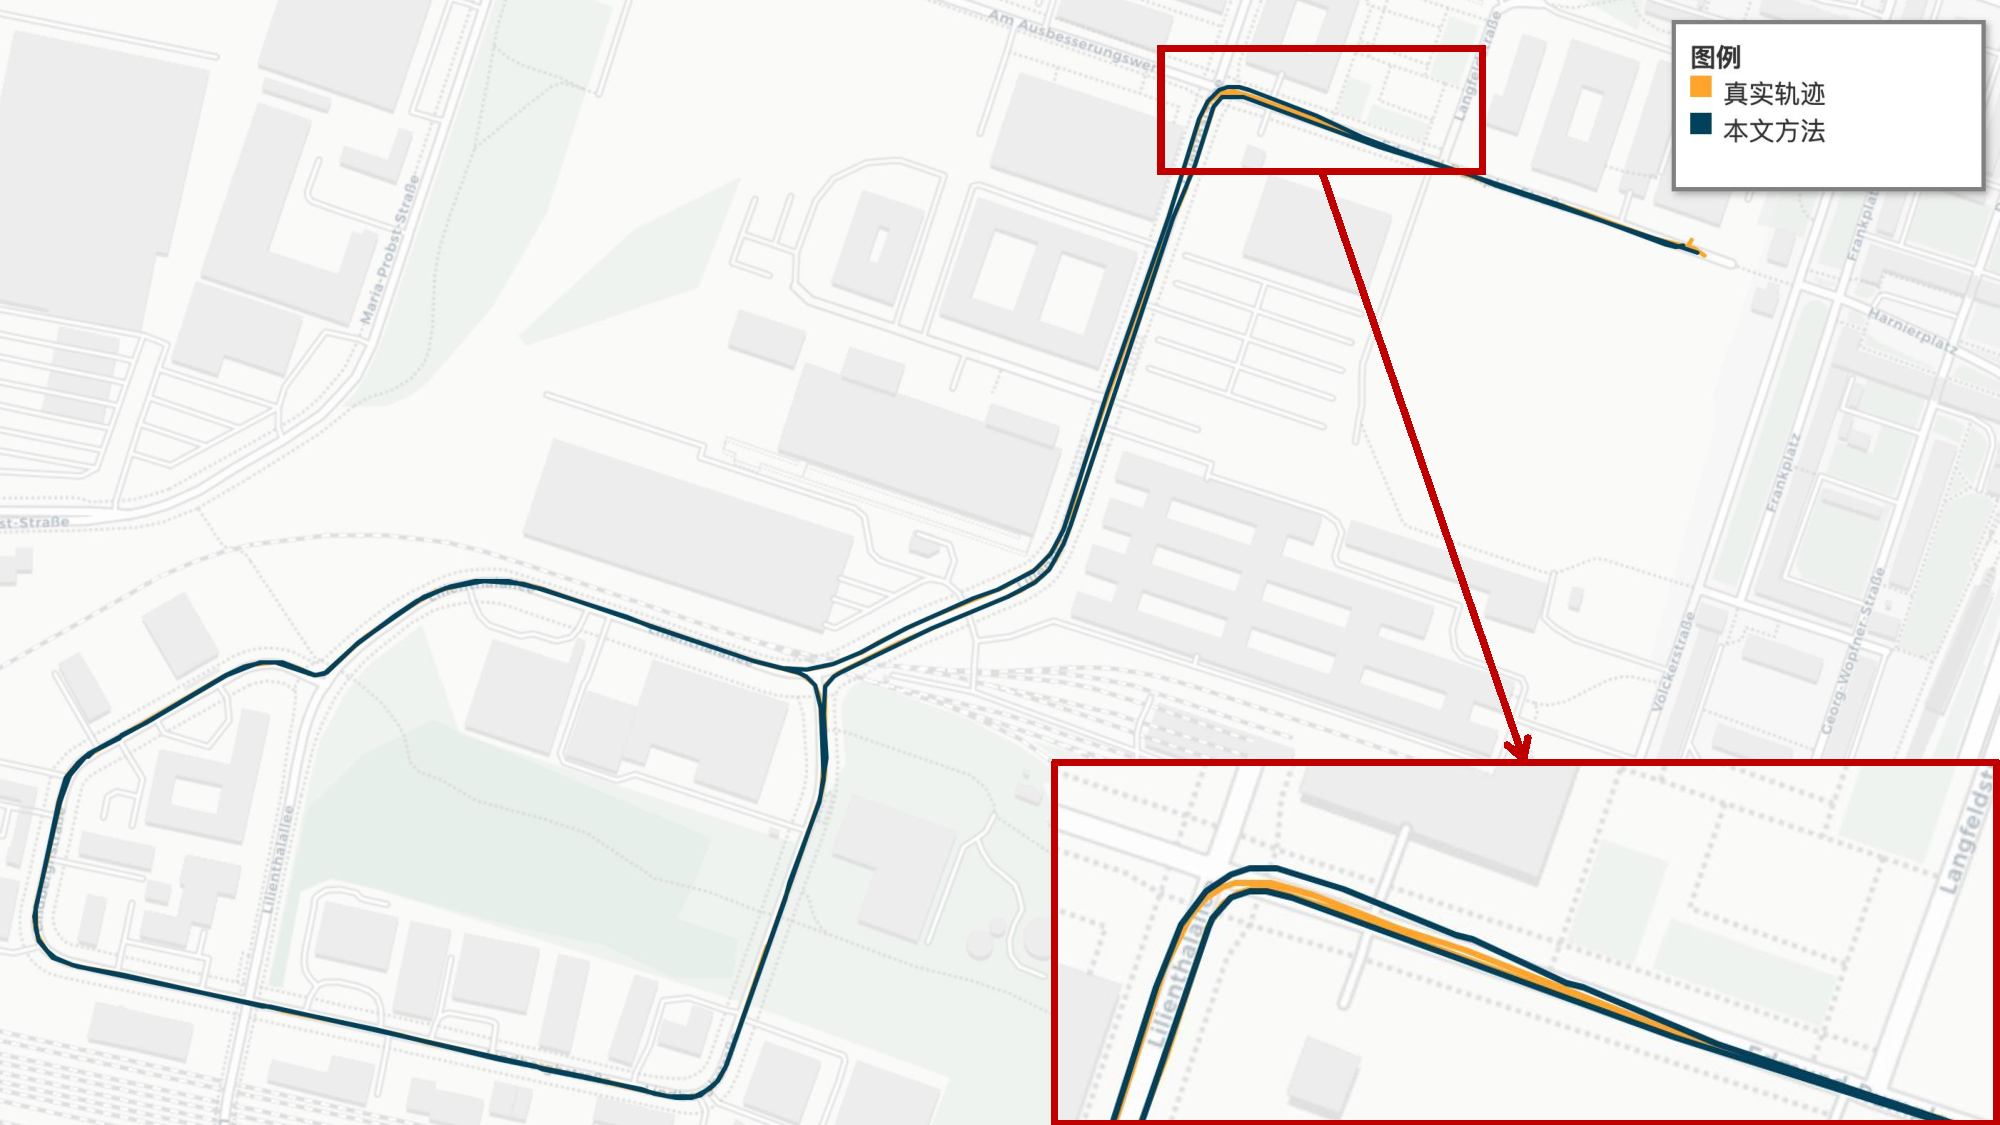
\includegraphics[width=0.45\linewidth]{OF2_zoomin.pdf}}
  \caption{本文系统在OF1序列上的建图轨迹与OF2序列上定位轨迹}
  \label{fig:loc_gnssmap}
\end{figure}

在图~\ref{fig:loc_4seasons_of2} 中可以看到在放大区域有着明显的定位误差,但这并非由于定位方法引入,而是由建图误差引入:如图~\ref{fig:loc_4seasons_of1} 所示,可以看到在定位误差较大的区域,建图时本身就存在明显的偏差,这导致了定位过程中引入了这一误差。因此,本文的定位方法在4Seasons数据集上的表现是受到了建图质量的影响,但是相较于其他方法,本文的定位方法在相同的建图条件下取得了更好的定位精度。

在Office Loop的环境下还有更多的具有挑战性的序列,本文在这些序列上也进行了测试。这些序列包括了OF3、OF4和OF5,具体的场景变化如图~\ref{fig:scene_of} 所示,这些序列的场景相较于OF2,有了晨昏~\ref{fig:scene_of3},季节~\ref{fig:scene_of4},天气~\ref{fig:scene_of5} 的变化。定位的结果如表~\ref{tab:loc_4seasons_of345} 所示,需要说明的是,由于从OF3开始场景出现了较大的变化,因此一些使用传统方法的地图定位方法无法再依靠地图信息运行,因此此处仅汇报了可以运行的方法。

% \begin{table}
% \centering
% \caption{4Seasons数据集Office Loop场景部分序列指标对比}
% \begin{tabular}{lccccccc}
% \toprule
% 方法                 & 时间                                                                             & 季节                  & 天气                  & 晨昏                  & $ATE_t$               & $RPE_t$              & $RPE_r$              \\ \midrule
% 离线建图               & \begin{tabular}[c]{@{}c@{}}03.24\\ 17:36\\ (OF1)\end{tabular}                  & 春季                  & 晴朗                  & 下午                  & 0.814881          & 0.929358          & 1.014480          \\ \midrule
% VINS-Mono          & \multirow{5}{*}{\begin{tabular}[c]{@{}c@{}}04.07\\ 10:20\\ (OF3)\end{tabular}} & \multirow{5}{*}{春季} & \multirow{5}{*}{晴朗} & \multirow{5}{*}{清晨} & 10.664015         & 5.305404          & 5.305404          \\
% ORB-SLAM3          &                                                                                &                     &                     &                     & 6.288431          & 5.000592          & 5.000592          \\
% VINS-Fusion w/ RTK &                                                                                &                     &                     &                     & 2.000104          & 3.678773          & 3.678773          \\
% VLS                &                                                                                &                     &                     &                     & 2.913034          & 3.978592          & 3.519618 \\
% 本文方法               &                                                                                &                     &                     &                     & \cellcolor[HTML]{FFCCC9}\textbf{0.938238} & \cellcolor[HTML]{FFCCC9}\textbf{2.947031} & \cellcolor[HTML]{FFCCC9}\textbf{2.529328} \\ \midrule
% VINS-Mono          & \multirow{5}{*}{\begin{tabular}[c]{@{}c@{}}06.12\\ 10:10\\ (OF4)\end{tabular}} & \multirow{5}{*}{夏季} & \multirow{5}{*}{晴朗} & \multirow{5}{*}{清晨} & 7.661955          & 3.447067          & 1.747575          \\
% ORB-SLAM3          &                                                                                &                     &                     &                     & 5.073350          & 3.207118          & 1.760357          \\
% VINS-Fusion w/ RTK &                                                                                &                     &                     &                     & 1.809687          & 2.158715          & 1.577418          \\
% VLS                &                                                                                &                     &                     &                     & 4.515426          & 8.142403          & 2.389229          \\
% 本文方法               &                                                                                &                     &                     &                     & \cellcolor[HTML]{FFCCC9}\textbf{0.792201} & \cellcolor[HTML]{FFCCC9}\textbf{1.402346} & \cellcolor[HTML]{FFCCC9}\textbf{1.047381} \\ \midrule
% VINS-Mono          & \multirow{5}{*}{\begin{tabular}[c]{@{}c@{}}01.07\\ 12:04\\ (OF5)\end{tabular}} & \multirow{5}{*}{冬季} & \multirow{5}{*}{降雪} & \multirow{5}{*}{下午} & 8.083566          & 2.598062          & \cellcolor[HTML]{FFCCC9}\textbf{0.990526} \\
% ORB-SLAM3          &                                                                                &                     &                     &                     & 5.520636          & 1.878826          & 1.000615          \\
% VINS-Fusion w/ RTK &                                                                                &                     &                     &                     & 2.448607          & 1.333865          & 0.934714          \\
% VLS                &                                                                                &                     &                     &                     & 1.862401          & 1.835533          & 0.999361          \\
% 本文方法               &                                                                                &                     &                     &                     & \cellcolor[HTML]{FFCCC9}\textbf{0.767040} & \cellcolor[HTML]{FFCCC9}\textbf{1.251208} & 0.999785          \\ \bottomrule
% \end{tabular}
% \label{tab:loc_4seasons_of345}
% \end{table}

具体分析此场景下的不同序列可以看出,OF3和OF1两个序列的分别是在下午和清晨拍摄,所以图片中的光照强度首先就有一定的不同,此外图~\ref{fig:scene_of1} 和图~\ref{fig:scene_of3}中道路的车况也有一定区别,在图~\ref{fig:scene_of3} 中出现了建图过程未出现的车辆,为定位的细粒度特征匹配增加了较大困难。

OF4和OF1两个序列存在季节的变化,从图~\ref{fig:scene_of1} 和图~\ref{fig:scene_of4} 中可以看到,OF4中的场景中出现了更繁茂的植被,甚至遮盖了部分建筑物,这对于细粒度特征匹配和定位都带来了一定的困难。OF5和OF1两个序列存在天气的变化,从图~\ref{fig:scene_of1} 和图~\ref{fig:scene_of5} 中可以看到,OF5中的场景中出现了降雪,改变了整个场景的整体感知条件,这对于定位的粗粒度和细粒度匹配都带来的挑战。

\begin{figure}
  \centering
  
\includegraphics[width=0.1\linewidth]{white.png}
  \subcaptionbox{OF1序列建图场景\label{fig:scene_of1}}{
    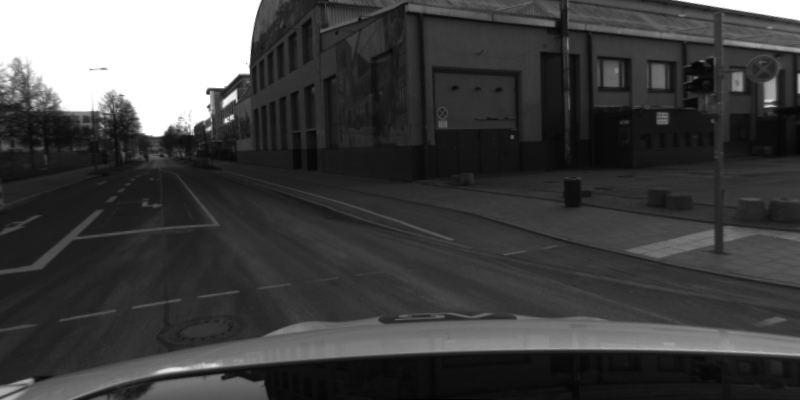
\includegraphics[width=0.32\linewidth]{OfficeLoop.png}
    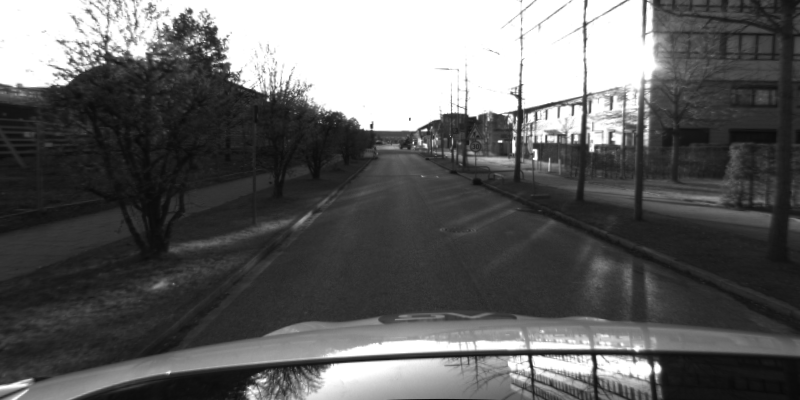
\includegraphics[width=0.32\linewidth]{OfficeLoop1_tree.png}}
  % 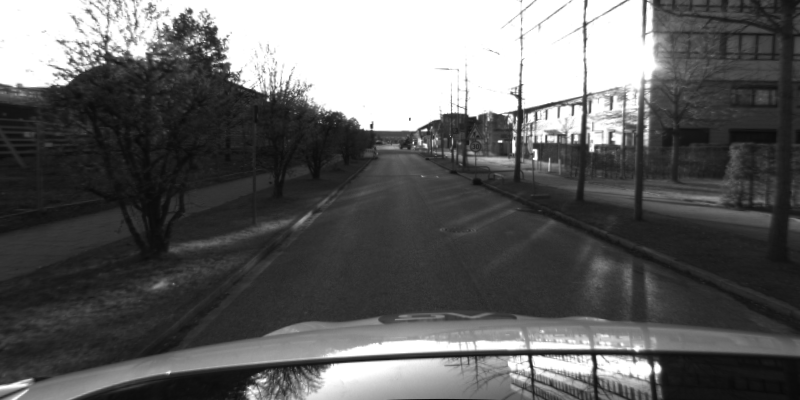
\includegraphics[width=0.32\linewidth]{OfficeLoop1_tree.png}
  
\includegraphics[width=0.1\linewidth]{white.png}
  \subcaptionbox{OF3序列清晨场景\label{fig:scene_of3}}{\includegraphics[width=0.32\linewidth]{OfficeLoop3.png}}
  \subcaptionbox{OF4序列夏季场景\label{fig:scene_of4}}{\includegraphics[width=0.32\linewidth]{OfficeLoop4.png}}
  \subcaptionbox{OF5序列冬季场景\label{fig:scene_of5}}{\includegraphics[width=0.32\linewidth]{OfficeLoop5.png}}
  \caption{4Seasons数据集OF3-5场景差异展示}
  \label{fig:scene_of}
\end{figure}

从表~\ref{tab:loc_4seasons_of345} 中的信息可以看出:本文方法在所有序列的$ATE_t$和$RPE_t$指标上均取得了明显的优势,是所有方法中唯一误差稳定在1米以内的方法;在OF5上的$RPE_r$指标上略逊于VINS-Fusion方法,但是差距极小。

\begin{table}
\centering
\caption{多种定位方法在OF3-5序列上的多指标对比}
\setlength{\tabcolsep}{3.2mm}{
\begin{tabular}{lccccccc}
\toprule
方法                 & 时间                                                                             & 季节                  & 天气                  & 晨昏                  & $ATE_t$               & $RPE_t$              & $RPE_r$              \\ \midrule
% 离线建图               & \begin{tabular}[c]{@{}c@{}}03.24\\ 17:36\\ (OF1)\end{tabular}                  & 春季                  & 晴朗                  & 下午                  & 0.81          & 0.92          & 1.01          \\ \midrule
VINS-Mono          & \multirow{5}{*}{\begin{tabular}[c]{@{}c@{}}04.07\\ 10:20\\ (OF3)\end{tabular}} & \multirow{5}{*}{春季} & \multirow{5}{*}{晴朗} & \multirow{5}{*}{清晨} & 10.66         & 5.30          & 5.30          \\
ORB-SLAM3          &                                                                                &                     &                     &                     & 6.28          & 5.00          & 5.00          \\
VINS-Fusion w/ RTK &                                                                                &                     &                     &                     & 2.00          & 3.67          & 3.67          \\
VLS                &                                                                                &                     &                     &                     & 2.91          & 3.97          & 3.51 \\
本文方法               &                                                                                &                     &                     &                     & \cellcolor[HTML]{FFCCC9}\textbf{0.93} & \cellcolor[HTML]{FFCCC9}\textbf{2.94} & \cellcolor[HTML]{FFCCC9}\textbf{2.52} \\ \midrule
VINS-Mono          & \multirow{5}{*}{\begin{tabular}[c]{@{}c@{}}06.12\\ 10:10\\(OF4)\end{tabular}} & \multirow{5}{*}{夏季} & \multirow{5}{*}{晴朗} & \multirow{5}{*}{清晨} & 7.66          & 3.44          & 1.74          \\
ORB-SLAM3          &                                                                                &                     &                     &                     & 5.07          & 3.20          & 1.76          \\
VINS-Fusion w/ RTK &                                                                                &                     &                     &                     & 1.80          & 2.15          & 1.57          \\
VLS                &                                                                                &                     &                     &                     & 4.51          & 8.14          & 2.38          \\
本文方法               &                                                                                &                     &                     &                     & \cellcolor[HTML]{FFCCC9}\textbf{0.79} & \cellcolor[HTML]{FFCCC9}\textbf{1.40} & \cellcolor[HTML]{FFCCC9}\textbf{1.04} \\ \midrule
VINS-Mono          & \multirow{5}{*}{\begin{tabular}[c]{@{}c@{}}01.07\\ 12:04\\ (OF5)\end{tabular}} & \multirow{5}{*}{冬季} & \multirow{5}{*}{降雪} & \multirow{5}{*}{下午} & 8.08          & 2.59          & 0.99 \\
ORB-SLAM3          &                                                                                &                     &                     &                     & 5.52          & 1.87          & 1.00          \\
VINS-Fusion w/ RTK &                                                                                &                     &                     &                     & 2.44          & 1.33          & \cellcolor[HTML]{FFCCC9}\textbf{0.93}          \\
VLS                &                                                                                &                     &                     &                     & 1.86          & 1.83          & 0.99          \\
本文方法               &                                                                                &                     &                     &                     & \cellcolor[HTML]{FFCCC9}\textbf{0.76} & \cellcolor[HTML]{FFCCC9}\textbf{1.25} & 0.99          \\ \bottomrule
\end{tabular}}
\label{tab:loc_4seasons_of345}
\end{table}

在表~\ref{tab:loc_4seasons_of2} 和表~\ref{tab:loc_4seasons_of345} 中还可以发现本文方法在地图本身具有误差的情况下,定位结果却出现了部分超越地图精度的情况。这一现象结合后文的消融实验可以看到本文将地图建模为概率地图的做法具有一定作用:在地图中引入了不确定性后,紧耦合优化可以更好地利用地图信息,从而提升定位精度。

为了更加直观得展示出定位的细节,本节还展示了在OF5序列上的粗粒度匹配与细粒度匹配结果:在OF5的定位序列中选择了4个具有代表性的位置进行展示,4个位置在轨迹上的分布以及各自的匹配结果展示,如图~\ref{fig:loc_4seasons_of5_details} 所示。粗粒度匹配的结果以图像对的形式展示:对比中将待定位的图像(上)与匹配的地图关键帧(下)进行了拼接,以探究粗粒度匹配的图像是否具有合理的共视关系。细粒度匹配的结果以特征点连线的形式展示:在粗粒度匹配图像的基础上,将图像中匹配的特征点进行了连线。粗粒度和细粒度匹配的结果可以表明:本文所使用的粗到细匹配方法在实际应用中有着良好的表现,即使在OF5序列中存在降雪的情况下,本文方法依然可以在粗粒度匹配中找到合理的共视关系,并且在细粒度匹配中也能找到足够的特征点进行匹配。

\begin{figure}
  \centering
  \includegraphics[width=1.0\linewidth]{localization_details.png}
  \caption{OF5序列上的粗粒度匹配与细粒度匹配结果}
  \label{fig:loc_4seasons_of5_details}
\end{figure}


\subsubsection{低结构化(Neighborhood)场景测试}

Neighborhood场景中有更多的植被,接近于农村环境,因此在这个场景下的测试能表现出本文方法在较低纹理环境下的表现。在此场景下又增加了几种Office Loop场景中没有出现的条件,例如降雨天气(NH3)和傍晚环境(NH7),如图~\ref{fig:scene_nh} 所示。测试结果如表~\ref{tab:loc_4seasons_nh23} 和表~\ref{tab:loc_4seasons_nh47} 所示。

\begin{figure}
\centering
\subcaptionbox{NH3序列降雨场景\label{fig:scene_nh3}}{\includegraphics[width=0.48\linewidth]{Neighborhood3.png}}
\subcaptionbox{NH7序列傍晚场景\label{fig:scene_nh7}}{\includegraphics[width=0.48\linewidth]{Neighborhood7.png}}
\caption{4Seasons数据集NH3与NH7场景差异展示}
\label{fig:scene_nh}
\end{figure}

% \begin{table}
% \centering
% \caption{4Seasons数据集Neighborhood场景第2与第3序列指标对比}
% \begin{tabular}{lccccccc}
% \toprule
% 方法                 & 时间                                                                             & 季节                  & 天气                  & 晨昏                  & $ATE_t$\textdownarrow{}               & $RPE_t$\textdownarrow{}              & $RPE_r$\textdownarrow{}              \\ \midrule
% 离线建图               & \begin{tabular}[c]{@{}c@{}}03.26\\ 13:32\\ (NH1)\end{tabular}                  & 春季                  & 多云                  & 下午                  & 0.133943          & 0.400299          & 0.451671          \\ \midrule
% ORB-SLAM3          & \multirow{4}{*}{\begin{tabular}[c]{@{}c@{}}10.07\\ 14:47\\ (NH2)\end{tabular}} & \multirow{4}{*}{秋季} & \multirow{4}{*}{多云} & \multirow{4}{*}{下午} & 3.896760          & 1.177058          & \cellcolor[HTML]{FFCCC9}\textbf{0.957432} \\
% VINS-Fusion w/ RTK &                                                                                &                     &                     &                     & 0.584860          & 2.081065          & 1.764747          \\
% VLS                &                                                                                &                     &                     &                     & 0.385877          & \cellcolor[HTML]{FFCCC9}\textbf{1.015101}          & 1.005846 \\
% 本文方法               &                                                                                &                     &                     &                     & \cellcolor[HTML]{FFCCC9}\textbf{0.325610} & 1.079635 & 1.022361          \\ \midrule
% ORB-SLAM3          & \multirow{4}{*}{\begin{tabular}[c]{@{}c@{}}10.07\\ 14:53\\ (NH3)\end{tabular}} & \multirow{4}{*}{秋季} & \multirow{4}{*}{降雨} & \multirow{4}{*}{下午} & 1.074461          & 1.193234          & \cellcolor[HTML]{FFCCC9}\textbf{0.980104} \\
% VINS-Fusion w/ RTK &                                                                                &                     &                     &                     & 0.557219          & 1.922972          & 1.199615          \\
% VLS                &                                                                                &                     &                     &                     & 0.338285          & 1.033000          & 1.002556          \\
% 本文方法               &                                                                                &                     &                     &                     & \cellcolor[HTML]{FFCCC9}\textbf{0.323113} & \cellcolor[HTML]{FFCCC9}\textbf{1.006227} & 1.006227          \\ \bottomrule
% \end{tabular}
% \label{tab:loc_4seasons_nh23}
% \end{table}

降雨条件和傍晚条件的感知条件如图~\ref{fig:scene_nh} 所示,左图的降雨条件可以看到明显的水雾出现在图像上,而右图的傍晚环境,可以看到明显的亮度降低。在这种条件下本文方法依旧在所有序列的$ATE_t$和$RPE_t$指标上取得了最好的效果,如表~\ref{tab:loc_4seasons_nh23} 和表~\ref{tab:loc_4seasons_nh47} 所示;虽然在$RPE_r$依旧没有比其他方法有明显优势,但是所有方法在该指标上的差距都非常小,更进一步展示了本文方法对环境的适应性强。

\begin{table}
\centering
\caption{多种定位方法在NH2与NH3序列上的多指标对比}
\setlength{\tabcolsep}{2.75mm}{
\begin{tabular}{lccccccc}
\toprule
方法                 & 时间                                                                             & 季节                  & 天气                  & 晨昏                  & $ATE_t$\textdownarrow{}               & $RPE_t$\textdownarrow{}              & $RPE_r$\textdownarrow{}              \\ \midrule
离线建图               & \begin{tabular}[c]{@{}c@{}}03.26\\ 13:32\\ (NH1)\end{tabular}                  & 春季                  & 多云                  & 下午                  & 0.13          & 0.40          & 0.45          \\ \midrule
ORB-SLAM3          & \multirow{4}{*}{\begin{tabular}[c]{@{}c@{}}10.07\\ 14:47\\ (NH2)\end{tabular}} & \multirow{4}{*}{秋季} & \multirow{4}{*}{多云} & \multirow{4}{*}{下午} & 3.89          & 1.17          & \cellcolor[HTML]{FFCCC9}\textbf{0.95} \\
VINS-Fusion w/ RTK &                                                                                &                     &                     &                     & 0.58          & 2.08          & 1.76          \\
VLS                &                                                                                &                     &                     &                     & 0.38          & \cellcolor[HTML]{FFCCC9}\textbf{1.01}          & 1.00 \\
本文方法               &                                                                                &                     &                     &                     & \cellcolor[HTML]{FFCCC9}\textbf{0.32} & 1.07 & 1.02          \\ \midrule
ORB-SLAM3          & \multirow{4}{*}{\begin{tabular}[c]{@{}c@{}}10.07\\ 14:53\\ (NH3)\end{tabular}} & \multirow{4}{*}{秋季} & \multirow{4}{*}{降雨} & \multirow{4}{*}{下午} & 1.07          & 1.19          & \cellcolor[HTML]{FFCCC9}\textbf{0.98} \\
VINS-Fusion w/ RTK &                                                                                &                     &                     &                     & 0.55          & 1.92          & 1.19          \\
VLS                &                                                                                &                     &                     &                     & 0.33          & 1.03          & 1.00          \\
本文方法               &                                                                                &                     &                     &                     & \cellcolor[HTML]{FFCCC9}\textbf{0.32} & \cellcolor[HTML]{FFCCC9}\textbf{1.00} & 1.00          \\ \bottomrule
\end{tabular}}
\label{tab:loc_4seasons_nh23}
\end{table}

在此场景下由于离线建图的精度较高,因此本文方法在定位过程中能够更好地利用地图信息,从而提升定位精度,$ATE_t$指标下都获得了30厘米左右的误差,已经达到了厘米级的定位精度。但是此场景下,本文定位方法并没有出现超越地图精度的情况,这主要是受限于本文定位方法的精度上限,这一上限也将在后文的消融实验中进行验证。

% \begin{table}
% \centering
% \caption{4Seasons数据集Neighborhood场景第4与第7序列指标对比}
% \begin{tabular}{lccccccc}
% \toprule
% 方法                 & 时间                                                                             & 季节                  & 天气                  & 晨昏                  & $ATE_t$\textdownarrow{}               & $RPE_t$\textdownarrow{}              & $RPE_r$\textdownarrow{}              \\ \midrule
% 离线建图               & \begin{tabular}[c]{@{}c@{}}03.26\\ 13:32\\ (NH1)\end{tabular}                  & 春季                  & 多云                  & 下午                  & 0.133943          & 0.400299          & 0.451671          \\ \midrule
% ORB-SLAM3          & \multirow{4}{*}{\begin{tabular}[c]{@{}c@{}}12.22\\ 11:54\\ (NH4)\end{tabular}} & \multirow{4}{*}{冬季} & \multirow{4}{*}{多云} & \multirow{4}{*}{清晨} & 3.326053          & 1.721227          & 1.014069          \\
% VINS-Fusion w/ RTK &                                                                                &                     &                     &                     & 0.584881          & 1.273095          & 1.337608          \\
% VLS                &                                                                                &                     &                     &                     & 0.336795          & 0.828517          & \cellcolor[HTML]{FFCCC9}\textbf{0.722960} \\
% 本文方法               &                                                                                &                     &                     &                     & \cellcolor[HTML]{FFCCC9}\textbf{0.303237} & \cellcolor[HTML]{FFCCC9}\textbf{0.787774} & 0.793884          \\ \midrule
% ORB-SLAM3          & \multirow{4}{*}{\begin{tabular}[c]{@{}c@{}}05.10\\ 18:32\\ (NH7)\end{tabular}} & \multirow{4}{*}{春季} & \multirow{4}{*}{多云} & \multirow{4}{*}{傍晚} & 1.770878          & 1.461675          & 1.239126          \\
% VINS-Fusion w/ RTK &                                                                                &                     &                     &                     & 1.098182          & 3.455674          & 2.230523          \\
% VLS                &                                                                                &                     &                     &                     & 0.304587          & 1.125579          & 1.007488          \\
% 本文方法               &                                                                                &                     &                     &                     & \cellcolor[HTML]{FFCCC9}\textbf{0.291957} & \cellcolor[HTML]{FFCCC9}\textbf{1.033805} & \cellcolor[HTML]{FFCCC9}\textbf{1.007318} \\ \bottomrule
% \end{tabular}
% \label{tab:loc_4seasons_nh47}
% \end{table}

\begin{table}
\centering
\caption{多种定位方法在NH4与NH7序列上的多指标对比}
\setlength{\tabcolsep}{2.75mm}{
\begin{tabular}{lccccccc}
\toprule
方法                 & 时间                                                                             & 季节                  & 天气                  & 晨昏                  & $ATE_t$\textdownarrow{}               & $RPE_t$\textdownarrow{}              & $RPE_r$\textdownarrow{}              \\ \midrule
% 离线建图               & \begin{tabular}[c]{@{}c@{}}03.26\\ 13:32\\ (NH1)\end{tabular}                  & 春季                  & 多云                  & 下午                  & 0.13          & 0.40          & 0.45          \\ \midrule
ORB-SLAM3          & \multirow{4}{*}{\begin{tabular}[c]{@{}c@{}}12.22\\ 11:54\\ (NH4)\end{tabular}} & \multirow{4}{*}{冬季} & \multirow{4}{*}{多云} & \multirow{4}{*}{清晨} & 3.3          & 1.72          & 1.01          \\
VINS-Fusion w/ RTK &                                                                                &                     &                     &                     & 0.58          & 1.27          & 1.33          \\
VLS                &                                                                                &                     &                     &                     & 0.33          & 0.82          & \cellcolor[HTML]{FFCCC9}\textbf{0.72} \\
本文方法               &                                                                                &                     &                     &                     & \cellcolor[HTML]{FFCCC9}\textbf{0.30} & \cellcolor[HTML]{FFCCC9}\textbf{0.78} & 0.79          \\ \midrule
ORB-SLAM3          & \multirow{4}{*}{\begin{tabular}[c]{@{}c@{}}05.10\\ 18:32\\ (NH7)\end{tabular}} & \multirow{4}{*}{春季} & \multirow{4}{*}{多云} & \multirow{4}{*}{傍晚} & 1.77          & 1.46          & 1.23          \\
VINS-Fusion w/ RTK &                                                                                &                     &                     &                     & 1.09          & 3.45          & 2.23          \\
VLS                &                                                                                &                     &                     &                     & 0.30          & 1.12          & \cellcolor[HTML]{FFCCC9}\textbf{1.00}          \\
本文方法               &                                                                                &                     &                     &                     & \cellcolor[HTML]{FFCCC9}\textbf{0.29} & \cellcolor[HTML]{FFCCC9}\textbf{1.03} & \cellcolor[HTML]{FFCCC9}\textbf{1.00} \\ \bottomrule
\end{tabular}}
\label{tab:loc_4seasons_nh47}
\end{table}

由于NH5和NH6所代表的环境已经在其他序列中出现,因此不再重复汇报其具体数值,而是以位移误差的云雨图~\ref{fig:loc_4seaons_nh5} 与云雨图~\ref{fig:loc_4seaons_nh6} 形式展示不同方法的定位结果。云雨图由小提琴图、箱线图、抖动散点图组合而成,展示了不同方法在NH5和NH6两个序列上的定位误差分布。可以看到本文方法在这两个序列上的定位误差分布更加集中,且中位数更低,这说明本文方法在这两个序列上的定位精度更高且更稳定。

\begin{figure}
  \centering
  \includegraphics[width=0.9\linewidth]{loc_NH5_cloud.png}
  \caption{多种定位方法在NH5序列上的定位误差分布}
  \label{fig:loc_4seaons_nh5}
\end{figure}

\begin{figure}
  \centering
  \includegraphics[width=0.9\linewidth]{loc_NH6_cloud.png}
  \caption{多种定位方法在NH6序列上的定位误差分布}
  \label{fig:loc_4seaons_nh6}
\end{figure}

% \begin{figure}
%   \centering
%   \includegraphics[width=1.0\linewidth]{loc_NH6_cloud.png}
%   \caption{不同定位方法在OF6序列上的定位误差分布}
%   \label{fig:loc_4seaons_nh6}
% \end{figure}

\subsubsection{复杂(Business Campus与Old Town)场景测试}

Business Campus场景在校园环境中,Old Town场景在城市中心区,这两个场景的有着更多的建筑物和道路,但也有着更多的移动物体和复杂的动态场景,如图~\ref{fig:scene_bc2} 和图~\ref{fig:scene_ot2} 所示,因此在这个场景下的测试能够更好地表现出本文方法在复杂环境下的表现。此外,在场景感知条件变化方面,这两个场景也覆盖了多种季节和天气条件,在Old Twon的建图序列中还有降雨天气,如图~\ref{fig:scene_ot1} 所示,也可以反映出本文方法在较差天气建图条件下的定位表现。

\begin{figure}
  \centering
  \subcaptionbox{BC2序列复杂场景\label{fig:scene_bc2}}{\includegraphics[width=0.32\linewidth]{BusinessCampus2.png}}
  \subcaptionbox{OT1序列降雨场景\label{fig:scene_ot1}}{\includegraphics[width=0.32\linewidth]{OldTown1.png}}
  \subcaptionbox{OT2序列复杂场景\label{fig:scene_ot2}}{\includegraphics[width=0.32\linewidth]{OldTown2.png}}
  \caption{4Seasons数据集NH3与NH7场景差异展示}
  \label{fig:scene_bcot}
\end{figure}

在两个场景下的对比如表~\ref{tab:loc_4seaons_bc56} 和表~\ref{tab:loc_4seaons_ot2} 所示,需要注意的是,由于Business Campus场景中的建图轨迹在进行$RPE_t$和$RPE_r$指标计算的时候,对齐过程数值不稳定产生了不合理结果,因此表中只给出了建图轨迹的$ATE_t$指标,可以看到该指标非常小,足以说明建图轨迹较为精确,因此另外两个指标的缺失也是可以接受的。本文方法依旧在$ATE_t$和$RPE_t$上取得了最佳表现,但是在$RPE_r$上表现不够稳定,但是与其他方法差距非常小。此外,在这两个场景下,本文方法在定位精度上依旧取得了1米以内的误差,这不仅说明本文方法在复杂场景下的表现优秀,也说明了本文方法具有较强的稳定性。

% \begin{table}
% \centering
% \caption{4Seasons数据集Business Campus场景部分序列指标对比}
% \begin{tabular}{lccccccc}
% \toprule
% 方法                 & 时间                                                                             & 季节                  & 天气                  & 晨昏                  & $ATE_t$\textdownarrow{}               & $RPE_t$\textdownarrow{}              & $RPE_r$\textdownarrow{}              \\ \midrule
% 离线建图               & \begin{tabular}[c]{@{}c@{}}10.08\\ 09:30\\ (BC1)\end{tabular}                  & 秋季                  & 晴朗                  & 清晨                  & 0.095337          & N/A               & N/A               \\ \midrule
% ORB-SLAM3          & \multirow{4}{*}{\begin{tabular}[c]{@{}c@{}}01.07\\ 13:12\\ (BC2)\end{tabular}} & \multirow{4}{*}{冬季} & \multirow{4}{*}{降雪} & \multirow{4}{*}{下午} & 7.376041          & 1.668179          & \cellcolor[HTML]{FFCCC9}\textbf{1.313357} \\
% VINS-Fusion w/ RTK &                                                                                &                     &                     &                     & 1.115755          & 2.313352          & 2.588801          \\
% VLS                &                                                                                &                     &                     &                     & 1.092215          & 1.938506          & 1.367412 \\
% 本文方法               &                                                                                &                     &                     &                     & \cellcolor[HTML]{FFCCC9}\textbf{0.639282} & \cellcolor[HTML]{FFCCC9}\textbf{1.576658} & 1.385713          \\ \midrule
% ORB-SLAM3          & \multirow{4}{*}{\begin{tabular}[c]{@{}c@{}}02.25\\ 14:16\\ (BC3)\end{tabular}} & \multirow{4}{*}{冬季} & \multirow{4}{*}{晴朗} & \multirow{4}{*}{下午} & 7.372700          & 1.760015          & 1.202648 \\
% VINS-Fusion w/ RTK &                                                                                &                     &                     &                     & 1.076147          & 2.596570          & 2.926574          \\
% VLS                &                                                                                &                     &                     &                     & 0.495447          & 2.025172          & 1.786391          \\
% 本文方法               &                                                                                &                     &                     &                     & \cellcolor[HTML]{FFCCC9}\textbf{0.446566} & \cellcolor[HTML]{FFCCC9}\textbf{1.380626} & \cellcolor[HTML]{FFCCC9}\textbf{1.109240}          \\ \bottomrule
% \end{tabular}
% \label{tab:loc_4seaons_bc56}
% \end{table}

\begin{table}
\centering
\caption{多种定位方法在Business Campus场景中的多指标对比}
\setlength{\tabcolsep}{2.75mm}{
\begin{tabular}{lccccccc}
\toprule
方法                 & 时间                                                                             & 季节                  & 天气                  & 晨昏                  & $ATE_t$\textdownarrow{}               & $RPE_t$\textdownarrow{}              & $RPE_r$\textdownarrow{}              \\ \midrule
离线建图               & \begin{tabular}[c]{@{}c@{}}10.08\\ 09:30\\ (BC1)\end{tabular}                  & 秋季                  & 晴朗                  & 清晨                  & 0.09          & N/A               & N/A               \\ \midrule
ORB-SLAM3          & \multirow{4}{*}{\begin{tabular}[c]{@{}c@{}}01.07\\ 13:12\\ (BC2)\end{tabular}} & \multirow{4}{*}{冬季} & \multirow{4}{*}{降雪} & \multirow{4}{*}{下午} & 7.37          & 1.66          & \cellcolor[HTML]{FFCCC9}\textbf{1.31} \\
VINS-Fusion w/ RTK &                                                                                &                     &                     &                     & 1.11          & 2.31          & 2.58          \\
VLS                &                                                                                &                     &                     &                     & 1.09          & 1.93          & 1.36 \\
本文方法               &                                                                                &                     &                     &                     & \cellcolor[HTML]{FFCCC9}\textbf{0.63} & \cellcolor[HTML]{FFCCC9}\textbf{1.57} & 1.38          \\ \midrule
ORB-SLAM3          & \multirow{4}{*}{\begin{tabular}[c]{@{}c@{}}02.25\\ 14:16\\ (BC3)\end{tabular}} & \multirow{4}{*}{冬季} & \multirow{4}{*}{晴朗} & \multirow{4}{*}{下午} & 7.37          & 1.76          & 1.20 \\
VINS-Fusion w/ RTK &                                                                                &                     &                     &                     & 1.07          & 2.59          & 2.92          \\
VLS                &                                                                                &                     &                     &                     & 0.49          & 2.02          & 1.78          \\
本文方法               &                                                                                &                     &                     &                     & \cellcolor[HTML]{FFCCC9}\textbf{0.44} & \cellcolor[HTML]{FFCCC9}\textbf{1.38} & \cellcolor[HTML]{FFCCC9}\textbf{1.10}          \\ \bottomrule
\end{tabular}}
\label{tab:loc_4seaons_bc56}
\end{table}

在Business Campus场景中,由于离线建图模块的精度较高,因此本文方法在定位过程中能够更好地利用地图信息,从而提升定位精度,$ATE_t$指标下都获得了50厘米左右的误差,已经有了较高的定位精度。

% \begin{table}
% \centering
% \caption{4Seasons数据集Old Town场景第2序列指标对比}
% \begin{tabular}{lccccccc}
% \toprule
% 方法                 & 时间                                                                             & 季节                  & 天气                  & 晨昏                  & $ATE_t$\textdownarrow{}               & $RPE_t$\textdownarrow{}              & $RPE_r$\textdownarrow{}              \\ \midrule
% 离线建图               & \begin{tabular}[c]{@{}c@{}}10.08\\11:53\\(OT1)\end{tabular}                  & 冬季                  & 降雨                  & 清晨                  & 1.016104          & 0.456781               & 1.116236               \\ \midrule
% ORB-SLAM3          & \multirow{4}{*}{\begin{tabular}[c]{@{}c@{}}02.25\\12:24\\(OT2)\end{tabular}} & \multirow{4}{*}{冬季} & \multirow{4}{*}{晴朗} & \multirow{4}{*}{清晨} & 38.930786         & 4.441040          & \cellcolor[HTML]{FFCCC9}\textbf{1.078154} \\
% VINS-Fusion w/ RTK &                                                                                &                     &                     &                     & 0.965686          & 2.682027          & 1.172853          \\
% VLS                &                                                                                &                     &                     &                     & 1.143163          & 2.318242          & 1.443211 \\
% 本文方法               &                                                                                &                     &                     &                     & \cellcolor[HTML]{FFCCC9}\textbf{0.846396} & \cellcolor[HTML]{FFCCC9}\textbf{2.318242} & 1.521039          \\ \bottomrule
% \end{tabular}
% \label{tab:loc_4seaons_ot2}
% \end{table}

\begin{table}
\centering
\caption{多种定位方法在Old Town场景中的多指标对比}
\setlength{\tabcolsep}{2.75mm}{
\begin{tabular}{lccccccc}
\toprule
方法                 & 时间                                                                             & 季节                  & 天气                  & 晨昏                  & $ATE_t$\textdownarrow{}               & $RPE_t$\textdownarrow{}              & $RPE_r$\textdownarrow{}              \\ \midrule
离线建图               & \begin{tabular}[c]{@{}c@{}}10.08\\11:53\\(OT1)\end{tabular}                  & 冬季                  & 降雨                  & 清晨                  & 1.01          & 0.45               & 1.11               \\ \midrule
ORB-SLAM3          & \multirow{4}{*}{\begin{tabular}[c]{@{}c@{}}02.25\\12:24\\(OT2)\end{tabular}} & \multirow{4}{*}{冬季} & \multirow{4}{*}{晴朗} & \multirow{4}{*}{清晨} & 38.93         & 4.44          & \cellcolor[HTML]{FFCCC9}\textbf{1.07} \\
VINS-Fusion w/ RTK &                                                                                &                     &                     &                     & 0.96          & 2.68          & 1.17          \\
VLS                &                                                                                &                     &                     &                     & 1.14          & 2.31          & 1.44 \\
本文方法               &                                                                                &                     &                     &                     & \cellcolor[HTML]{FFCCC9}\textbf{0.84} & \cellcolor[HTML]{FFCCC9}\textbf{2.31} & 1.52          \\ \bottomrule
\end{tabular}}
\label{tab:loc_4seaons_ot2}
\end{table}

但是在Old Town场景中,由于建图序列的天气情况较差,所以轨迹的精度较低,而在这种条件下本文的定位方法依旧达到了1米以内的定位精度,这说明本文方法对于建图质量的要求并不十分苛刻,在较差的建图精度下还可以通过定位给出更加精确的结果。

\subsection{消融实验}

为了验证地图定位模块中的各个部分对定位精度的影响,本节进行了一系列的消融实验。在这些实验中,本节逐步增加地图定位模块中的各个过程,从而验证了这些过程对定位精度的影响。具体实验结果如表~\ref{tab:loc_ablation} 所示,表中主要研究了“PO-VIO”、“粗到细定位”、“转换矩阵更新”、“相邻帧边”、“地图关键帧边”、“地图观测边”、“地图点先验边”和“真值地图”这8个过程对定位精度的影响,实验设置在Office Loop的第3条序列(OF3)上,以$ATE_t$为主要报告指标。

% \begin{table}
% \centering
% \begin{threeparttable}
% \caption{消融实验结果对比}
% \begin{tabular}{ccccccccc}
% \toprule
% PO-VIO          & \begin{tabular}[c]{@{}c@{}}粗到细\\ 定位\end{tabular} & \begin{tabular}[c]{@{}c@{}}转换矩阵\\ 更新\end{tabular} & \begin{tabular}[c]{@{}c@{}}相邻帧\\ 边\end{tabular} & \begin{tabular}[c]{@{}c@{}}地图\\ 关键帧边\end{tabular} & \begin{tabular}[c]{@{}c@{}}地图\\ 观测边\end{tabular} & \begin{tabular}[c]{@{}c@{}}地图点\\ 先验边\end{tabular} & \begin{tabular}[c]{@{}c@{}}真值 \\ 地图 \end{tabular} & $ATE_t$    \\ \midrule
% $\checkmark$ &                                                  &                                                   &                                                 &                                                   &                                                  &                                                   &                                                 & 17.193425      \\
%               & $\checkmark$                                     &                                                   &                                                 &                                                   &                                                  &                                                   &                                                 & \textgreater{}60     \\
% $\checkmark$ & $\checkmark$                                     &                                                  &                                                 &                                                   &                                                  &                                                   &                                                 & \underline{6.987066} \\
% $\checkmark$ & $\checkmark$                                     &$\checkmark$                                                   &                                                 &                                                   &                                                  &                                                   &                                                 & 1.898881 \\
% $\checkmark$ & $\checkmark$                                     &$\checkmark$                                                   & $\checkmark$                                    &                                                   &                                                  &                                                   &                                                 & 1.445279       \\
% $\checkmark$ & $\checkmark$                                     &$\checkmark$                                                   & $\checkmark$                                    & $\checkmark$                                      &                                                  &                                                   &                                                 & 1.237693       \\
% $\checkmark$ & $\checkmark$                                     &$\checkmark$                                                   & $\checkmark$                                    & $\checkmark$                                      & $\checkmark$                                     &                                                   &                                                 & 1.223113       \\
% $\checkmark$ & $\checkmark$                                     &$\checkmark$                                                   & $\checkmark$                                    & $\checkmark$                                      & $\checkmark$                                     & $\checkmark$                                      &                                                 & 0.938238       \\
% $\checkmark$ & $\checkmark$                                     &$\checkmark$                                                   & $\checkmark$                                    & $\checkmark$                                      & $\checkmark$                                     & $\checkmark$                                      & $\checkmark$                                    & 0.396039       \\ \bottomrule
% \end{tabular}
% \label{tab:loc_ablation}
% \begin{tablenotes}
%   \item [a] 实验构建在Office Loop的第3条序列(OF3)上
%   \item [b] \underline{下划线}表示该序列在后期因为转换矩阵未更新而粗到细定位失败
% \end{tablenotes}
% \end{threeparttable}
% \end{table}

\begin{table}
\centering
\begin{threeparttable}
\caption{地图定位模块的消融实验结果}
\begin{tabular}{ccccccccc}
\toprule
PO-VIO          & \begin{tabular}[c]{@{}c@{}}粗到细\\ 定位\end{tabular} & \begin{tabular}[c]{@{}c@{}}转换矩阵\\ 更新\end{tabular} & \begin{tabular}[c]{@{}c@{}}相邻帧\\ 边\end{tabular} & \begin{tabular}[c]{@{}c@{}}地图\\ 关键帧边\end{tabular} & \begin{tabular}[c]{@{}c@{}}地图\\ 观测边\end{tabular} & \begin{tabular}[c]{@{}c@{}}地图点\\ 先验边\end{tabular} & \begin{tabular}[c]{@{}c@{}}真值 \\ 地图 \end{tabular} & $ATE_t$    \\ \midrule
$\checkmark$ &                                                  &                                                   &                                                 &                                                   &                                                  &                                                   &                                                 & 17.19      \\
              & $\checkmark$                                     &                                                   &                                                 &                                                   &                                                  &                                                   &                                                 & \textgreater{}60     \\
$\checkmark$ & $\checkmark$                                     &                                                  &                                                 &                                                   &                                                  &                                                   &                                                 & \underline{6.98} \\
$\checkmark$ & $\checkmark$                                     &$\checkmark$                                                   &                                                 &                                                   &                                                  &                                                   &                                                 & 1.89 \\
$\checkmark$ & $\checkmark$                                     &$\checkmark$                                                   & $\checkmark$                                    &                                                   &                                                  &                                                   &                                                 & 1.44       \\
$\checkmark$ & $\checkmark$                                     &$\checkmark$                                                   & $\checkmark$                                    & $\checkmark$                                      &                                                  &                                                   &                                                 & 1.23       \\
$\checkmark$ & $\checkmark$                                     &$\checkmark$                                                   & $\checkmark$                                    & $\checkmark$                                      & $\checkmark$                                     &                                                   &                                                 & 1.22       \\
$\checkmark$ & $\checkmark$                                     &$\checkmark$                                                   & $\checkmark$                                    & $\checkmark$                                      & $\checkmark$                                     & $\checkmark$                                      &                                                 & 0.93       \\
$\checkmark$ & $\checkmark$                                     &$\checkmark$                                                   & $\checkmark$                                    & $\checkmark$                                      & $\checkmark$                                     & $\checkmark$                                      & $\checkmark$                                    & 0.31       \\ \bottomrule
\end{tabular}
\label{tab:loc_ablation}
\begin{tablenotes}
  \item [a] 实验构建在Office Loop的第3条序列(OF3)上。
  \item [b] \underline{下划线}表示该序列在后期因为转换矩阵未更新而粗到细定位失败。
\end{tablenotes}
\end{threeparttable}
\end{table}

在表~\ref{tab:loc_ablation} 中只有“粗到细定位”时产生了较大的定位误差,这是因为粗到细定位在没有先验位置信息辅助的时候,其粗定位过程仅使用粗粒度特征易产生误匹配,从而将整个定位误差增长到了一个难以接受的程度。在第三行,当使用了PO-VIO和转换矩阵后,这一定位误差极大得缩小到了一个可以接受的程度,这说明本文使用的转换矩阵具有非常重要的作用。但是在仅有转换矩阵而不维护的情况下,在序列的后段,由于PO-VIO的累积误差越来越大,使得转换矩阵不再能准确反映当前VIO结果和全局坐标系的正确关系,此时粗到细定位的先验位置信息也失去了意义,所以定位失败,因此表中的数据以\underline{下划线}表示其是不完整序列的定位数据。在加入了转换矩阵更新之后,轨迹不完整的问题得到了解决,定位精度得到了进一步的提升。

在第5-8行中,逐步加入了相邻帧边、地图关键帧边、地图观测边和地图点先验边,可以看到这些边的加入都使得定位精度得到了进一步的提升,这说明这些边对于定位精度的提升都是有益的。这表明本文所提出的紧耦合优化中的各个残差边都是对定位结果有正向作用的。

在最后一行中,加入了真值地图,可以看到定位精度得到了进一步的提升,这说明真值地图对于定位精度的提升是有益的。在使用了真值地图后,定位精度达到了30厘米左右,这可以看作是本文方法的定位精度上限,而这也与4Seasons数据集中实验情况相符:在建图精度不足的情况下,本文方法的精度上限受到地图精度的限制(例如Office Loop场景和Old Town场景),但是在建图精度较高的情况下,本文方法的定位精度上限只由紧耦合地图定位模块的精度决定(例如Neighborhood场景和Business Campus场景)。

\subsection{系统效率与成本分析}

\subsubsection{效率分析}

对于固定路线定位系统来说,效率是与精度同样重要的评价指标,因此针对地图定位系统的运行效率进行了展示与分析,如表~\ref{tab:loc_efficiency} 所示。具体来说,此处对地图定位模块中的各个过程进行了运行时间分析。主要的耗时过程包括:粗特征提取、粗特征匹配、细特征提取+匹配、概率投票定位、(紧耦合位姿图)优化。其中前四项均为粗到细视觉定位方法所涉及的过程,其中粗特征提取和细特征提取+匹配均涉及到神经网络的推理,因此分别展示了这些过程在TensorRT和PyTorch两个神经网络推理框架下的推理时间,并使用特殊符号${\dagger}$着重表示;粗特征匹配和概率投票定位均不需要神经网络,因此并不区分推理框架。此外,整个系统中另一个时间占用显著的过程是优化,因此也单独进行时间测试,其他过程由于单独耗时可以忽略,因此合计为一项。

\begin{table}
\centering
\begin{threeparttable}
\caption{地图定位模块的运行时间(毫秒)测试}
\setlength{\tabcolsep}{2.9mm}{
\begin{tabular}{lccccccc}
\toprule
推理框架     & \begin{tabular}[c]{@{}c@{}}$^{\dagger}$粗特征\\ 提取\end{tabular} & \begin{tabular}[c]{@{}c@{}}粗特征\\ 匹配\end{tabular} & \begin{tabular}[c]{@{}c@{}}$^{\dagger}$细特征\\ 提取+匹配\end{tabular} & \begin{tabular}[c]{@{}c@{}}概率投票\\ 定位\end{tabular} & 优化                   & 其他                   & 总计    \\ \midrule
TensorRT & 9.0                                              & \multirow{2}{*}{0.4}                             & 4.2+20.1                                            & \multirow{2}{*}{3.5}                              & \multirow{2}{*}{1.4} & \multirow{2}{*}{0.1} & 38.7  \\
PyTorch  & 22.2                                             &                                                  & 59.8+242.6                                          &                                                   &                      &                      & 330.0 \\ \bottomrule
\end{tabular}}
\label{tab:loc_efficiency}
\begin{tablenotes}
  \item [a] ${\dagger}$表示此过程使用神经网络类方法。
\end{tablenotes}
\end{threeparttable}
\end{table}

通过表中数据的对比,可以清晰地看出本文方法中神经网络的时间开销是非常大的,尤其是在PyTorch框架下,细特征提取+匹配的时间开销达到了300ms以上,而整体的运行时间也达到了330ms,这意味着如果使用PyTorch框架进行本文方法的部署,那么在同等硬件条件下定位的频率也只能保持3Hz左右。而在TensorRT框架下,细特征提取+匹配的时间开销仅为30ms左右,整体的运行时间也仅为38ms,这说明本文使用TensorRT框架来支持地图定位模块是非常必要的。同时也证明本文系统具有实际可用的效率表现:在使用TensorRT框架的情况下,定位频率可以达到25Hz左右,可以满足绝大多数的实时定位需求。

\subsubsection{成本分析}

为了分析本文所提出系统在精度和成本方面的综合表现,表~\ref{tab:loc_cost} 中展示了当前集中主流定位方案的传感器配置、精度和成本,为了使对比更加公平且真实,每一种方案都列举了一种公开的商业产品型号。

\begin{table}
\centering
\begin{threeparttable}
\caption{地图定位模块的使用成本分析}
\begin{tabular}{lcccccc}
\toprule
产品型号                                                                                       & 定位方法       & 位置 & 姿态 & 传感器价格          & 持续服务     & 精度上限  \\ \midrule
北天BS-357\cite{BS-357}                                                                                   & 单频GNSS     &  $\checkmark$  &     & \textyen100            & N/A      & 5.00m    \\
千寻SV100\cite{SV100}                                                                                    & RTK        &  $\checkmark$  &    & \textyen12,100          & \textyen2,400/套/年 & 0.02m \\
千寻GJ-A802\cite{GJ-A802}                                                                                  & GNSS/INS   &  $\checkmark$  &  $\checkmark$  & \textyen19,200          & \textyen2,400/套/年 & 0.02m \\
\rowcolor{gray!20} 传感器组合 & 本文系统 &  $\checkmark$  &  $\checkmark$  & \textyen7,467 & N/A      & 0.30m  \\ \bottomrule 
% \rowcolor{gray!20} Gemini 2 L\cite{Gemini-2L}& 本文方法 &  $\checkmark$  &  $\checkmark$  &  \textyen 2,200           & N/A      & 0.3m  \\ \bottomrule
\end{tabular}
\label{tab:loc_cost}
\begin{tablenotes}
  \item [a] 传感器组合使用了Basler acA2040-35gm\cite{acA2040-35gm}相机和Analog Devices ADIS16465\cite{ADIS16465}IMU。
\end{tablenotes}
\end{threeparttable}
\end{table}

在表中,单频GNSS定位方案的精度上限为5米,价格为\textyen100,是所有定位方案中价格最低的形式。但是其存在的问题也非常明显:首先是精度差,最高5米的精度是所有方案中最差的,而且由于误差绝对值较大,在高级的车辆或轮式机器人应用中难以使用;其次是其功能仅限定位,没有可靠的姿态估计方案。

RTK的定位方案相较于单频GNSS方案已经有了较大的精度提升,达到了厘米级别。但是其高昂的价格以及持续服务的费用,以千寻SV100\cite{SV100}为例,其价格为\textyen12,100,持续服务费用为\textyen2,400/套/年,这使得其部署成本高昂,尤其是在大规模的应用中。此外RTK的定位方案也仅限于位置估计,无法估计高精度姿态。

GNSS/INS组合定位方案补全了RTK方案中姿态估计的缺失,但是其更高昂的硬件成本以及持续服务费用使定位成本大幅提高。

本文方法需要依赖传感器组合,即相机和IMU来实现,因此其成本主要集中于传感器价格。以本文4Seasons数据集实验中的传感器为例,相机与IMU的组合价格为\textyen7,467,而本文系统在此传感器配置的基础上实现了30厘米的精度上限。虽然这一精度相较于RTK和GNSS/INS组合定位方案的精度上限有所差距,但是本文系统在传感器价格和持续服务方面有着明显的成本优势。

综上所述,本文系统在精度和成本方面取得了较好的平衡:即以较低的价格实现了足够的精度上限,且不需要持续服务费用,这使得本文系统具有大规模部署的潜力。


\section{本章总结}

本章主要以实验验证的方式对本文所提出的固定路线定位系统进行评估。首先,本章对实验实施的环境进行了介绍,包括实验所使用的数据集、实验所使用的硬件平台和软件平台以及实验的评估指标,包括绝对轨迹误差和相对姿态误差。然后本章分别针对3个模块的性能进行了测试:在建图模块测试中,本文所设计的建图方法在KITTI数据集上取得了优于单纯SfM和视觉-GNSS松耦合方法的精度,基本保持在厘米级精度;在PO-VIO模块测试中,本文方法在多个数据集的绝对位移误差和相对角度误差上均取得了相较基线和其他方法的优势表现,相对位移误差的劣势是由于相关变量梯度缺乏监督导致的;在地图定位模块测试中,本文方法在多个场景中均取得了厘米级的绝对定位精度,这一表现甚至优于一些高精度的视觉-GNSS融合方法。最后,本章还对本文方法的效率和成本进行了分析,证明了本文方法在精度和成本方面取得了较好的平衡。
\chapter{总结与展望}

\section{论文总结}

固定路线中的视觉惯性定位是一项在自动驾驶、工业巡检等领域有着广泛需求的技术。但是当前的定位技术依赖于高成本的高精地图或者高精度传感器,这都严重制约了其在大规模应用中的推广。

为了解决这一问题,本文提出了一种基于视觉惯性的固定路线定位系统,该系统不依赖于人工标注的高精地图和昂贵的传感器,在建图阶段只需要图像和高精度的GNSS信息,在定位阶段只需要使用低成本的相机和IMU传感器,即可完成整个从建图到定位的流程。在建图到定位的整个流程中,本文需要解决的问题包括:(1)如何利用图像和GNSS信息构建具有可接受精度的地图;(2)如何融合IMU和相机信息进行较高精度的位姿估计;(3)如何使用地图和相对位姿估计结果进行更精确的定位任务。针对这三个问题,本文提出了一个完整的固定路线中的视觉惯性定位系统,包括:

(1)基于视觉和位置信息融合的离线建图模块。为了克服以往SLAM建图过程全局优化不足的问题,本文提出了一种基于SfM和GNSS融合的先验地图构建方法。首先对图片和 GNSS 信息进行预处理,筛选出候选关键帧,并进行语义分割等操作;紧接着对纯图像进行 SfM 以获得在视觉建图世界坐标系下的相机位姿和地图点云;然后使用 GNSS 信息和 SfM 结果进行建图对齐,即实现视觉建图世界坐标系和全局坐标系的对齐;此后进行建图融合,以非线性优化的方式同时优化视觉重投影误差和 GNSS 提供的位置误差;最后输出分层次的的地图。

(2)基于车身运动模式感知的伪观测视觉惯性里程计(PO-VIO)模块。为了解决以往通用视觉惯性里程计方法在车辆或轮式机器人上的速度估计不合理问题,本文设计了一种更符合车辆或轮式机器人运动状态的视觉惯性里程计:在通用VIO的基础上,本文引入了车辆在直行时车身横向和垂直速度为0的伪观测,依据IMU的序列数据和基于深度学习的车身运动模式判别方法来检测车身状态变化,在特定状态下完成惯性-车体对齐并加入伪观测约束,从而获得更精确的相对位姿。

(3)基于最大后验概率的地图定位模块。为了能够充分使用地图观测信息和视觉惯性里程计信息,本文设计了一种基于最大后验概率的,同步优化位姿与地图的紧耦合地图定位模块。整个模块首先通过比较图像观测与地图信息,利用粗粒度的图像特征和位置先验信息确定初步位置范围,再通过细粒度的像素特征匹配获得更精确的相机位姿。同时,通过转换矩阵初始化和初始位姿自适应选择来对齐视觉惯性里程计和地图观测,并验证地图定位结果的有效性。最终,通过将定位问题建模为最大后验概率估计,并以位姿图优化的形式求解最终定位结果,通过不断更新转换参数来防止PO-VIO累积误差对整个系统的负面影响。

本文在公开数据集上对提出的系统进行了大量的实验验证,实验结果表明,本文提出的固定路线中的视觉惯性定位系统在定位精度和鲁棒性上均优于当前主流的视觉惯性定位方法。具体而言,本文系统在建图阶段即可将建图精度控制在1米以内;在里程计模块中,本文所提出的PO-VIO模块能够显著改善绝对位置误差至5米以内,改善相对角度误差至每100米1$\degree$以内;在地图定位模块中,能够达到最高30厘米以内的绝对位移误差误差;整个系统的在线部分单帧推理时延,在深度学习加速库的帮助下最高可以降至40毫秒左右,这表明了本文系统具有实际部署的可行性,并且其具有较好的实用性和可推广性。

\section{未来展望}

在未来,本文考虑在以下几个方向进行进一步的研究:

(1)当前的研究中使用地图作为重要的观测来源,但是每次使用时并不会对地图进行更新,这在长时间的使用中可能会导致地图的过时。因此,未来可以考虑在定位过程中对地图进行增量式更新,以提高地图的实时性和准确性。

(2)本文在研究过程中发现动态物体对定位精度有较大的影响,因此未来可以考虑在定位过程中对动态物体进行检测和处理,以提高定位的鲁棒性。

(3)基于深度学习的状态检测方法在本文的视觉惯性里程计部分发挥了重要作用,但是这种使用方法过于简单,未来考虑在更多的环节加入深度学习技术,以提高定位的精度和鲁棒性。


% 其他部分
\backmatter

% 参考文献
\bibliography{ref/refs}  % 参考文献使用 BibTeX 编译
% \printbibliography       % 参考文献使用 BibLaTeX 编译

% 附录
% 本科生需要将附录放到声明之后,个人简历之前
\appendix
% \input{data/appendix-survey}       % 本科生:外文资料的调研阅读报告
% \input{data/appendix-translation}  % 本科生:外文资料的书面翻译
% !TeX root = ../thuthesis-example.tex

\chapter{补充内容}
% \label{appendix:quat}

\section{四元数与旋转矩阵转换}
\label{appendix:quat}
设单位四元数为
\begin{equation}
\symbf{q} = q_w + q_x i + q_y j + q_z k,
\end{equation}
满足归一化条件
\begin{equation}
q_w^2 + q_x^2 + q_y^2 + q_z^2 = 1.
\end{equation}
对应的旋转矩阵 \(\symbf{R}\) 可由下式给出:
\begin{equation}
  \symbf{R} = \begin{bmatrix}
1 - 2(q_y^2 + q_z^2) & 2(q_xq_y - q_zq_w) & 2(q_xq_z + q_yq_w) \\
2(q_xq_y + q_zq_w) & 1 - 2(q_x^2 + q_z^2) & 2(q_yq_z - q_xq_w) \\
2(q_xq_z - q_yq_w) & 2(q_yq_z + q_xq_w) & 1 - 2(q_x^2 + q_y^2)
\end{bmatrix}.
\end{equation}
给定旋转矩阵 \(\symbf{R} = [R_{ij}]\),可以通过下列方式提取四元数(其中一种常用的方法):
\begin{align}
  q_w &= \frac{1}{2}\sqrt{1 + R_{11} + R_{22} + R_{33}},\\
  q_x &= \frac{R_{32} - R_{23}}{4q_w},\\
  q_y &= \frac{R_{13} - R_{31}}{4q_w},\\
  q_z &= \frac{R_{21} - R_{12}}{4q_w}.
\end{align}

以上公式仅适用于单位四元数,且在实际应用中可能需要对数值稳定性进行进一步处理。


\section{光束法平差雅可比矩阵与优化}
\label{appendix:bundle_adjustment}
假设三维点 \( \mathbf{p} = (X, Y, Z)^T \) 在相机坐标系下的坐标为 \( \mathbf{p}_c \),其投影到图像平面上的像素坐标为 \( \mathbf{p} = (u, v)^T \)。相机的内参矩阵为 \( \mathbf{K} \),旋转矩阵为 \( \mathbf{R} \),平移向量为 \( \mathbf{t} \)。则有:
\begin{equation}
\mathbf{p}_c = \mathbf{R} \mathbf{p} + \mathbf{t}
\end{equation}
\begin{equation}
\mathbf{x} = \mathbf{K} \begin{bmatrix}
\frac{X_c}{Z_c} \\
\frac{Y_c}{Z_c} \\
1
\end{bmatrix}
\end{equation}
其中,\( \mathbf{p}_c = (X_c, Y_c, Z_c)^T \) 为三维点在相机坐标系下的坐标。
重投影误差 \( \mathbf{e} \) 定义为:
\begin{equation}
\mathbf{e} = \mathbf{x} - \mathbf{x}_{\text{obs}}
\end{equation}
其中,\( \mathbf{x}_{\text{obs}} \) 为实际观测到的像素坐标。
为了进行优化,需要计算重投影误差对旋转 \( \mathbf{R} \)、平移 \( \mathbf{t} \) 和地图点 \( \mathbf{P} \) 的雅可比矩阵。利用链式法则,雅可比矩阵可以分解为以下部分:
\begin{equation}
\frac{\partial \mathbf{e}}{\partial \mathbf{R}} = \frac{\partial \mathbf{e}}{\partial \mathbf{x}} \cdot \frac{\partial \mathbf{x}}{\partial \mathbf{p}_c} \cdot \frac{\partial \mathbf{p}_c}{\partial \mathbf{R}}
\end{equation}

\begin{equation}
\frac{\partial \mathbf{e}}{\partial \mathbf{t}} = \frac{\partial \mathbf{e}}{\partial \mathbf{x}} \cdot \frac{\partial \mathbf{x}}{\partial \mathbf{p}_c} \cdot \frac{\partial \mathbf{p}_c}{\partial \mathbf{t}}
\end{equation}

\begin{equation}
\frac{\partial \mathbf{e}}{\partial \mathbf{p}} = \frac{\partial \mathbf{e}}{\partial \mathbf{x}} \cdot \frac{\partial \mathbf{x}}{\partial \mathbf{p}_c} \cdot \frac{\partial \mathbf{p}_c}{\partial \mathbf{p}}
\end{equation}
其中,各部分的雅可比矩阵为:
\begin{equation}
\frac{\partial \mathbf{e}}{\partial \mathbf{x}} = \mathbf{I}_{2 \times 2}
\end{equation}

\begin{equation}
\frac{\partial \mathbf{p}}{\partial \mathbf{p}_c} = \mathbf{K} \cdot \begin{bmatrix}
\frac{1}{Z_c} & 0 & -\frac{X_c}{Z_c^2} \\
0 & \frac{1}{Z_c} & -\frac{Y_c}{Z_c^2} \\
0 & 0 & 0
\end{bmatrix}
\end{equation}

\begin{equation}
\frac{\partial \mathbf{p}_c}{\partial \mathbf{R}} = -\mathbf{R} \cdot \left[ \mathbf{p} \right]_\times
\end{equation}

\begin{equation}
\frac{\partial \mathbf{p}_c}{\partial \mathbf{t}} = \mathbf{I}_{3 \times 3}
\end{equation}

\begin{equation}
\frac{\partial \mathbf{p}_c}{\partial \mathbf{p}} = \mathbf{R}
\end{equation}
其中,\( \left[ \mathbf{p} \right]_\times \) 表示向量 \( \mathbf{P} \) 的反对称矩阵:
\begin{equation}
\left[ \mathbf{p} \right]_\times = \begin{bmatrix}
0 & -Z & Y \\
Z & 0 & -X \\
-Y & X & 0
\end{bmatrix}
\end{equation}
将上述各部分雅可比矩阵相乘,即可得到重投影误差对旋转、平移和地图点的雅可比矩阵。

高斯-牛顿法是一种用于求解非线性最小二乘问题的迭代算法。其目标是找到参数向量 \( \mathbf{x} \),使得残差的平方和最小化。具体而言,目标函数可以表示为:
\begin{equation}
F(\mathbf{x}) = \frac{1}{2} \sum_{i=1}^{m} r_i^2(\mathbf{x})
\end{equation}
其中,\( r_i(\mathbf{x}) \) 表示第 \( i \) 个残差函数,\( m \) 为残差的数量。
为了最小化 \( F(\mathbf{x}) \),我们需要找到使其梯度为零的 \( \mathbf{x} \)。首先,计算目标函数的梯度:
\begin{equation}
\nabla F(\mathbf{x}) = \sum_{i=1}^{m} r_i(\mathbf{x}) \nabla r_i(\mathbf{x})
\end{equation}
其中,\( \nabla r_i(\mathbf{x}) \) 是残差函数 \( r_i(\mathbf{x}) \) 关于 \( \mathbf{x} \) 的梯度。
接下来,对每个残差函数 \( r_i(\mathbf{x}) \) 进行一阶泰勒展开:
\begin{equation}
r_i(\mathbf{x} + \Delta \mathbf{x}) \approx r_i(\mathbf{x}) + \nabla r_i(\mathbf{x})^T \Delta \mathbf{x}
\end{equation}
将其代入目标函数的梯度表达式,得到:
\begin{equation}
\nabla F(\mathbf{x} + \Delta \mathbf{x}) \approx \sum_{i=1}^{m} \left[ r_i(\mathbf{x}) + \nabla r_i(\mathbf{x})^T \Delta \mathbf{x} \right] \nabla r_i(\mathbf{x})
\end{equation}
为了使梯度为零,需要解以下线性方程组:
\begin{equation}
\mathbf{J}(\mathbf{x})^T \mathbf{r}(\mathbf{x}) + \mathbf{J}(\mathbf{x})^T \mathbf{J}(\mathbf{x}) \Delta \mathbf{x} = 0
\end{equation}
其中,\( \mathbf{J}(\mathbf{x}) \) 是残差函数的雅可比矩阵,\( \mathbf{r}(\mathbf{x}) \) 是所有残差的向量表示。
解上述方程组,得到参数更新量:
\begin{equation}
\Delta \mathbf{x} = -\left[ \mathbf{J}(\mathbf{x})^T \mathbf{J}(\mathbf{x}) \right]^{-1} \mathbf{J}(\mathbf{x})^T \mathbf{r}(\mathbf{x})
\end{equation}
然后,更新参数:
\begin{equation}
\mathbf{x} \leftarrow \mathbf{x} + \Delta \mathbf{x}
\end{equation}
重复上述步骤,直到满足收敛条件。


\section{罗德里格斯旋转公式}
\label{appendix:rodrigues}
罗德里格斯旋转公式给定一个旋转矩阵 \( \symbf{R} \),可以将其转换为旋转向量 \( \boldsymbol{\theta} = \theta \symbf{u} \),其中 \( \theta \) 是旋转角度,\( \symbf{u} \) 是旋转轴的单位向量。旋转角度 \( \theta \)的计算方式如下:

\begin{equation}
\theta = \cos^{-1} \left( \frac{\text{trace}(\symbf{R}) - 1}{2} \right)
\end{equation}
其中,\( \text{trace}(\symbf{R}) \) 表示矩阵 \( \symbf{R} \) 的迹,即对角线元素之和。旋转轴 \( \symbf{u} \)是一个单位向量,其计算方式为:
\begin{equation}
\symbf{u} = \frac{1}{2 \sin \theta} \begin{bmatrix}
\symbf{R}_{32} - \symbf{R}_{23} \\
\symbf{R}_{13} - \symbf{R}_{31} \\
\symbf{R}_{21} - \symbf{R}_{12}
\end{bmatrix}
\end{equation}
其中,\( \symbf{R}_{ij} \) 表示矩阵 \( \symbf{R} \) 的第 \( i \) 行第 \( j \) 列元素。




% 致谢
% !TeX root = ../thuthesis-example.tex

\begin{acknowledgements}

清华求学三年,首先要感谢的是我的父母,是你们的多年供养让我能专心读书与科研;家庭作为我的支持,我倍感温暖和安心。还要感谢张凯老师,张凯老师是我研究生学习生涯的指路明灯:张老师不仅在专业方面对我有谆谆教诲,更是在人生选择和人格塑造方面对我有深刻影响。同时感谢数信院的老师们、华为中央媒体技术院的专家们,感谢你们在不同阶段给过我的指导和关心。

我还要感谢我一路同行的朋友和伙伴们,是你们让我的求学经历不再孤单。感谢同门的罗奇、陈子龙、王一博、邬豪杰、叶宇辰、卢汉卿、赵千淇和吴丹彤等同学,与你们的讨论和交流经常让我茅塞顿开,收获新发现与新思考;感谢郑钊宇、刘瑜平、罗赵彤和袁玉红等师兄师姐,你们的经验和指导使我在学习和研究中多了几分安心和从容。特别感谢丁桦同学,你在我三年的求学过程中给我面对困难的勇气,给我焦虑中的宽慰,给我痛苦中的关爱……你的存在让我在这个孤独的世界勇敢地走下去!

最后我还想感谢母校清华大学,感谢你对我人生观和世界观的塑造。回首求学的来时路,早年最令我印象深刻的一篇文章是《闻一多先生的说和做》:“他,是口的巨人。他,是行的高标”,这臧克家对闻一多先生的评价,也是我一生追求的人生目标。在清华,“行胜于言”的精神更为我的追求增加了一份使命感和荣誉感。在清华的日子很快就要结束了,但是我深感践行清华精神的旅程才刚刚开始,行胜于言将会是我日后时时自省的标尺。

无愧言行,无愧母校,吾当勉励!

\end{acknowledgements}


% 声明
% 本科生开题报告不需要
\statement
% 将签字扫描后的声明文件 scan-statement.pdf 替换原始页面
% \statement[file=scan-statement.pdf]
% 本科生编译生成的声明页默认不加页脚,插入扫描版时再补上;
% 研究生编译生成时有页眉页脚,插入扫描版时不再重复。
% 也可以手动控制是否加页眉页脚
% \statement[page-style=empty]
% \statement[file=scan-statement.pdf, page-style=plain]

% 个人简历、在学期间完成的相关学术成果
% 本科生可以附个人简历,也可以不附个人简历
% !TeX root = ../thuthesis-example.tex

\begin{resume}

  \section*{个人简历}

  1999 年 04 月 21 日出生于山东淄博博山区。

  2017 年 9 月考入大连理工大学电信学部计算机科学与技术(日语强化)专业,2022 年 7 月本科毕业并获得工学学士学位。

  2022 年 9 月免试进入清华大学深圳国际研究生院攻读大数据技术与工程专业硕士至今。


  \section*{在学期间完成的相关学术成果}

  \subsection*{学术论文}

  \begin{achievements}
    \item \textbf{Linsong Xue}, Luo Qi, Zhang Kai. APM-SLAM: Visual Localization for Fixed Routes with Tightly Coupled A Priori Map. Journal of Intelligent and Connected Vehicles[J]. (审稿中)
    \item \textbf{Linsong Xue}, Kai Zhang, Guowei Zhu. Visual Localization with Prior Map. ITS World Congress 2025[C]. (审稿中)
    \item Haojie Wu, \textbf{Linsong Xue}, Kai Zhang. SGAGS: Semantic-Guided Adaptive 3D Gaussian Splatting. In press[C]. (已被 the 5th International Conference on Image, Vision and Intelligent Systems录用)
  \end{achievements}


  \subsection*{专利}

  \begin{achievements}
    \item 张凯, 薛林松, 鹿昌义, 等. 一种间断GNSS信号下的车辆融合定位方法及相关设备: 中国, CN118112623A[P]. 2024-05-31.
    \item 张凯, 薛林松, 鹿昌义, 等. 一种基于NRTK和视觉信息的巡检车定位系统: 中国, CN119022939A[P]. 2024-11-26.
  \end{achievements}

\end{resume}


% 指导教师/指导小组评语
% 本科生不需要
% !TeX root = ../thuthesis-example.tex

\begin{comments}
% \begin{comments}[name = {指导小组评语}]
% \begin{comments}[name = {Comments from Thesis Supervisor}]
% \begin{comments}[name = {Comments from Thesis Supervision Committee}]

论文选题聚焦于固定路线中的定位技术,在实际生活生产中具有广泛的应用前景。论文工作围绕视觉惯性定位方法展开,提出了一种基于先验地图和多传感器融合的定位系统,完成了地图构建、视觉惯性定位增强以及地图定位等多项工作,设计了一种完整的固定路线中视觉惯性定位系统,并通过多场景数据严谨论证了系统性能,包括精度和效率等方面。

论文的贡献包括:(1) 提出了基于 SfM 和 GNSS 融合的离线建图模块,有效得做到了建图成本与精度之间的平衡;(2) 提出了基于车身运动模式感知的伪观测视觉惯性里程计模块,有效得将车身的运动学先验融合到了视觉惯性里程计中;(3) 提出了基于概率地图的地图定位模块,有效得提升了定位精度和效率;(4) 通过多场景数据验证了系统效果,系统在精度和效率上均优于现有的视觉惯性定位系统以及地图定位系统。

论文显示该学生掌握了相关领域的知识,基础扎实,具有一定的独立研究能力;论文结构清晰,思路严谨,论证得当,写作规范,符合学术论文的要求,达到硕士学位论文要求。同意参加硕士论文答辩。

\end{comments}


% 答辩委员会决议书
% 本科生不需要
% !TeX root = ../thuthesis-example.tex

\begin{resolution}

  

\end{resolution}


% 本科生的综合论文训练记录表(扫描版)
% \record{file=scan-record.pdf}

\end{document}
